\documentclass[11pt]{ociamthesis}  % default square logo 
%\documentclass[12pt,beltcrest]{ociamthesis} % use old belt crest logo
%\documentclass[12pt,shieldcrest]{ociamthesis} % use older shield crest logo
\usepackage[top=1.3in, bottom=1.25in, left=1.2in, right=1.2in]{geometry}
\usepackage{fancyhdr}
\newcommand{\HH}{\ensuremath{\PH\PH}}
\newcommand{\mHH}{\ensuremath{M_{\PH\PH}}\xspace}
\newcommand{\Hgg}{\ensuremath{\PH\to\gamma\gamma}}
\newcommand{\Hbb}{\ensuremath{\PH\to b\bar{b}}}
\newcommand{\ggbb}{\ensuremath{b\bar{b}\gamma\gamma}}
\newcommand{\bbgg}{\ensuremath{b\bar{b}\gamma\gamma }}
\newcommand{\bbbb}{\ensuremath{b\bar{b}b\bar{b}}}
\newcommand{\ggjj}{\ensuremath{\gamma\gamma jj}}
\newcommand{\jjgg}{\ensuremath{jj\gamma\gamma}}
\newcommand{\gjjj}{\ensuremath{\gamma jjj}}
%\newcommand{\Mggjjk}{\ensuremath{m_{\gamma\gamma {\rm jj}}^{\rm kin}}}
%\newcommand{\pTj}{\ensuremath{p_{T, {\rm jet}}}}
\newcommand{\Mx}{\ensuremath{M_{\mathrm{X}}}\xspace}
\newcommand{\Mtilde}{\ensuremath{\tilde{M}_{\mathrm{X}}}\xspace}
\newcommand{\Mgg}{\ensuremath{M(\gamma\gamma)}\xspace}
\newcommand{\Mjj}{\ensuremath{M(jj)}\xspace}
\newcommand{\Mjjr}{\ensuremath{M_(jj)^{r}}}
%\newcommand{\Mjjr}{\ensuremath{M_{\rm jj}^{\rm r}}}
\newcommand{\thetastar}{\ensuremath{\theta^{\rm CS}_{\rm HH}}}
\newcommand{\acosthetastar}{\ensuremath{|\cos {\theta^{\rm CS}_{\rm HH}}|}}
\newcommand{\Mggjj}{\ensuremath{M(jj\gamma\gamma)}}
\newcommand{\Mjjgg}{\ensuremath{M(jj\gamma\gamma)}}
%\newcommand{\Mggjj}{\ensuremath{M_{\gamma\gamma {\rm jj}}}}
\newcommand{\Mggjjk}{\ensuremath{M(\gamma\gammajj)_{kin}}}
\newcommand{\Mjjggk}{\ensuremath{M(jj\gamma\gamma)_{kin}}}
%\newcommand{\Mggjjk}{\ensuremath{M_{\gamma\gamma {\rm jj}}^{\rm kin}}}
\newcommand{\Mggjjrk}{\ensuremath{M(\gamma\gammajj)_{kin}^{r}}}
\newcommand{\Mjjggrk}{\ensuremath{M(jj\gamma\gamma)_{kin}^{r}}}
%\newcommand{\Mggjjrk}{\ensuremath{M_{\gamma\gamma {\rm jj}}^{\rm r, kin}}}
\newcommand{\pT}{\ensuremath{p_{T}}\xspace}
\newcommand{\pTj}{\ensuremath{p_{T, {\rm jet}}}}
\newcommand{\pTjr}{\ensuremath{p_{T, {\rm jet}}^r}}
\newcommand{\kapt}{\ensuremath{\kappa_{t}}}
\newcommand{\kapl}{\ensuremath{\kappa_{\lambda}}}
\newcommand{\ctwo}{\ensuremath{c_2}}
\newcommand{\sieie}{\ensuremath{\sigma_{i\eta i\eta}}}
\newcommand{\ctwog}{\ensuremath{c_{2g}}\xspace}
\newcommand{\cg}{\ensuremath{c_g}\xspace}
\newcommand{\sigmaHH}{\ensuremath{\sigma_{\PH\PH}}\xspace}
\newcommand{\sigmaHHSMNNLO}{\ensuremath{\sigma_{\PH\PH}^{\textrm SM,NNLO}}\xspace}
\newcommand{\DeltaR}{\ensuremath{\Delta{\textrm R}}\xspace}
\def\met{\mbox{${\hbox{$E$\kern-0.45em\lower-.1ex\hbox{\bf{/}}}}_T$}\xspace} %missing ET                                                                                 
\def \gmet  {$\gamma$ + \met}
%\def \pt {p$_\text{T}$~}
\def \zinvg  {Z($\nu\bar{\nu}$)+$\gamma$~}
\def \winlvg  {W($\ell\nu$)+$\gamma$~}
\def \sigieie  {$\sigma_{\text{i}{\eta}\text{i}{\eta}}~$}
\def \sigipip  {$\sigma_{\text{i}{\phi}\text{i}{\phi}}~$}
\newcommand{\as}{$\alpha_s$~}
\newcommand{\comm}[1]{}
\def \etg {E$_\text{T}^{\gamma}$\xspace}
\def\met{\mbox{${\hbox{$E$\kern-0.45em\lower-.1ex\hbox{\bf{/}}}}_T$}\xspace} %missing ET
\def \gmet  {$\gamma$ + \met\xspace}
%\def \pt {p$_\text{T}$~}
\def \zinvg  {Z($\nu\bar{\nu}$)+$\gamma$\xspace}
\def \winlvg  {W($\ell\nu$)+$\gamma$\xspace}
\def \sigieie  {$\sigma_{\text{i}{\eta}\text{i}{\eta}}\xspace$}
\def \sigipip  {$\sigma_{\text{i}{\phi}\text{i}{\phi}}\xspace$}
\newcommand{\Pgg}{\ensuremath{{\gamma}}}
\newcommand{\Pe}{\ensuremath{{e}}}
\newcommand{\Pep}{\ensuremath{{e}^+}}
\newcommand{\Pem}{\ensuremath{{e}^-}}
\providecommand{\Pgn}{\ensuremath{\nu}}
\providecommand{\Pagn}{\ensuremath{\overline{\nu}}}
\newcommand{\PW}{\ensuremath{\mathrm{W}}}
\providecommand{\PSGczDo}{\ensuremath{\widetilde{\chi}^{0}_{1}}\xspace} % neutralino

\def\HZg{$H\to Z\gamma$\xspace}
%\def\Hgg{$H\to\gamma\gamma$\xspace}
\def\HWWllnn{$H\to WW \to ll \nu\nu$\xspace}
\def\HWW{$H\to WW$\xspace}

\newcommand{\pb} {\,\mathrm{pb}\xspace}
\newcommand{\PXXG}{\ensuremath{G}\xspace} % graviton
\newcommand{\PXXSG}{\ensuremath{\widetilde{\PXXG}}\xspace} % gravitino
\newcommand{\PSGc}{\ensuremath{\widetilde{\chi}}\xspace} % neutralino



%load any additional packages
\usepackage{amssymb}
\usepackage[hidelinks]{hyperref}
\usepackage{ptdr-definitions}
\extrafloats{100}
\usepackage{array}
\usepackage{float}
\usepackage{multirow}
\usepackage{graphbox}


%input macros (i.e. write your own macros file called mymacros.tex 
%and uncomment the next line)
%\include{mymacros}

%\title{Shedding a light: \\[1ex]
%         Beyond the Standard Model Higgs Physics with Photons at CMS}

\title{Beyond the Standard Model Higgs Physics with Photons with the CMS Detector}


%\title{Searches for Di-Higgs Production in the $b\bar{b}\gamma\gamma$ Final State\\[1ex]     %your thesis title,
%        with the CMS Run-2 Dataset}   %note \\[1ex] is a line break in the title

\author{Rafael Teixeira de Lima}             %your name
%\college{St Catherine's College}  %your college

%\renewcommand{\submittedtext}{change the default text here if needed}
\degree{Doctor of Philosophy}     %the degree
\degreedate{April 11, 2017}         %the degree date
%\usepackage[applemac]{inputenc}
\usepackage[portuges,brazilian,french,english]{babel}
\usepackage[T1]{fontenc}
\usepackage[section]{placeins}

%end the preamble and start the document
\begin{document}
\begin{romanpages}          % start roman page numbering
\maketitleneu                  % create a title page from the preamble info
%\begin{copyrightEnv}\end{copyrightEnv}

%%Path to figures
%\graphicspath{{./hh/figures/}}

%set the number of sectioning levels that get number and appear in the contents
\setcounter{secnumdepth}{3}
\setcounter{tocdepth}{2}

\begin{dedication}
\noindent
\,\,\,\,\,\, To the ones that came beside me, \\
To all the lost at land and sea, \\
To the wanderers under the night sky, \\
And the dreamers who have lost their seed

\vspace{.5cm}

To the broken bones and ragged mind \\
Healing off in Amazonian delight \\
To the old ones that are here again \\
Looping over colored mandalas of zen

\vspace{.5cm}

To the tough chocolate bossa nova \\
From whom life takes me away over and over \\
To the latin blood in Mexican dressing \\
The harbinger of my astrological blessings

\vspace{.5cm}

To the lily of the valley that springs on the ice \\
Where airbags and whiskey can complete a life \\
And also to the ones of whom I think not often, \\
Some things are meant to be forgotten

\vspace{.5cm}

To the bumps and jumps and lumps \\
Of things I throw away or save for a rainy day \\
When I remember the ones that came beside me \\
I bow at this end, my friends, and I thank thee

\vspace*{\fill}
\begin{flushright}
Para a minha m�e.
\end{flushright}

\end{dedication}        % include a dedication.tex file
\begin{acknowledgementslong}

First and foremost, I would like to thank my Ph.D. advisor, Prof. Toyoko Orimoto, for her encouragement and support, particularly at tough times. 
After spending almost four years based at CERN hearing horror stories about life-draining and mind-destroying Ph.D. advisors, I consider myself extremely lucky to have worked with someone who would push me into new projects and adventures while still considering my well-being. 

I would like to thank the second in command, one of the most upbeat people I have ever met, Italian kitchen master and ECAL connoisseur Andrea Massironi. 
A good part of what I have learned during my years at CERN were from white-board conversations with him and/or at pizza parties. 

I would like to thank the ECAL DAQ team, particularly Giacomo Cucciati. Learning the ropes of the ECAL online software while cheering in the office whenever the code compiled was surely a great way to work.

I would like to thank, in general, the ECAL team, and, specifically, David Barney, Andr� David, Evgueni Vlassov, David Petyt and Pedro Parracho. Their expertise is only surpassed by their willingness to teach newcomers about the wonders of ECAL.

I would like to thank the $b\bar{b}\gamma\gamma$ team, specially Amina Zghiche and Alexandra Carvalho, for the support and encouragement even when the energies were gone but there was still a lot to do. 

I would also like to thank the Northeastern HEP team, specially Profs. Darien Wood and Emanuela Barberis, for their continuous useful input and discussions during our group meetings. And to Bruno, Dina, Mark and Mitchell, who made my one year in Boston an unforgettable experience.

A special warm thanks to Rafael Coelho Lopes de S�, who followed me from D0 to CMS so he could continue teaching me about particle physics and the wonders of the academic life. His help during the always-so-difficult job-searching period probably kept me from throwing my laptop against a wall a couple of times. 

Brenda, Brisa, Rebeca and Yasmin, you know the drill. 

Finalmente, agrade�o a minha m�e, Roseane Teixeira de Lima, que me apoia mesmo se eu deixar de ligar para ela na hora em que sempre combinamos - ela sabe que n�o fa�o por mal. 
Mas agrade�o especialmente a ela pela minha forma��o como uma pessoa de sonhos e objetivos concretos, e que trabalha por eles. 
A minha m�e foi o meu primeiro exemplo de que as coisas melhoram com trabalho duro e dedica��o. 
As coisas melhoraram tanto que ela j� conheceu v�rios pa�ses da Europa e vai voltar para mais.

\end{acknowledgementslong}   % include an acknowledgements.tex file

%this baselineskip gives sufficient line spacing for an examiner to easily
%markup the thesis with comments
%\baselineskip=18pt plus1pt


\begin{abstract}
plenty of waffle, plenty of waffle, plenty of waffle, plenty of waffle,
plenty of waffle, plenty of waffle, plenty of waffle, plenty of waffle.
\end{abstract}          % include the abstract

\renewcommand{\contentsname}{Table of Contents}
\tableofcontents            % generate and include a table of contents
%\listoffigures              % generate and include a list of figures
\end{romanpages}            % end roman page numbering

%now include the files of latex for each of the chapters etc
\pagestyle{fancy}
\fancyhf{}
\rfoot{\thepage}
\rhead{\rightmark}

\chapter{Introduction}
\graphicspath{{introduction/figures/}{introduction/}}


\section{The Standard Model of Particle Physics}

The Standard Model of particles and fields (SM) describes the most basic constituents of matter and their dynamics, as currently known. 
It is built upon the hypothesis that fundamental, point-like particles exist (fermions) and that their interactions, via bosonic fields, can be described in a relativistic quantum field theoretical framework. 
Fundamental interactions are described in the SM by the gauge invariance principle, meaning that interactions will appear in the framework as gauge fields after imposing local and continuous (gauge) symmetries. 
An early example of this principle is the emergence of electromagnetism on the Schr�dinger equation by imposing a local and continuous $U(1)$ symmetry.

As of today, the SM described three types of interactions: 

\begin{description}
\item[The Strong Interaction] Also known as quantum chromodynamics or QCD. It appears in the SM via an $SU(3)$ gauge symmetry. This gauge group implies the existence of 8 gauge bosons, called gluons. Fermions particles that interact via QCD are called \textbf{quarks}, and are organized in triplets of a "color" charge. Fermions that do not interact via QCD are called \textbf{leptons}. 

\item[The Electromagnetic Interaction] It appears in the SM via an $U(1)$ gauge symmetry, with one gauge boson associated to it (photon). The particles that interact via the electromagnetic interaction have electric charge. 

\item[The Weak Interaction] Appears in the SM via an $SU(2)$ gauge symmetry. It has three different gauge bosons associated to it, two have electric charge: $W^{+}$ and $W^{-}$, while one is neutral: $Z^{0}$. The weak interaction charge is commonly called weak hypercharge.
\end{description}

The two last interactions have been further combined in a single theoretical model, called the electroweak interaction  \cite{weinberg_ew, salam_ew, glashow_ew}. 
It is based on the fact that, before a spontaneous symmetry breaking occurs, both interactions can be described by a single gauge group, namely $SU(2)\otimes U(1)$. 
A main ingredient of this unification process is the spontaneous symmetry breaking mechanism based on the Higgs field \cite{englert_brout,guralnik,higgs}. 

The organization of the field content of the SM was completed with the observation that both quarks and leptons are organized into three generations. 
The first generation of leptons contains the electron ($e$) and the electron neutrino ($\nu_e$), while the first generation of quarks contains the up quark ($u$) and the down quark ($d$). 
The second generation of leptons contains the muon ($\mu$) and the mu neutrino ($\nu_{\mu}$), while the second generation of quarks contains the charm quark ($c$) and the strange quark ($s$). 
The third generation of leptons contains the tau ($\tau$) and the tau neutrino ($\nu_{\tau}$), while the third generation of quarks contains the top quark ($t$) and the bottom quark ($b$). 
The generation structure is particularly important by noting that particles of the same family, with left-handed chirality, form a weak isospin doublet, while the right-handed fermions are weak singlets: 

\begin{equation}
\begin{array}{ccc}
L_{l}=\left(\begin{array}{c}
\nu_{e}\\
e
\end{array}\right)_{L}, & \left(\begin{array}{c}
\nu_{\mu}\\
\mu
\end{array}\right)_{L}, & \left(\begin{array}{c}
\nu_{\tau}\\
\tau
\end{array}\right)_{L};\\
\\
L_{q}=\left(\begin{array}{c}
u\\
d
\end{array}\right)_{L}, & \left(\begin{array}{c}
c\\
s
\end{array}\right)_{L}, & \left(\begin{array}{c}
t\\
b
\end{array}\right)_{L};
\end{array}
\end{equation}



\begin{equation}
R_l = e_{R},\,\mu_{R},\,\tau_{R};\, \, R_q = u_{R},\, d_{R},\, c_{R},\, s_{R},\, t_{R},\, b_{R}.
\end{equation}



\section{The Electroweak Theory of Glashow-Weinberg-Salam}

Through observations that date back to the early XX century, the electroweak interactions were built upon a set of experimental fundaments:

\begin{description}
\item[Universality] The weak interactions are blind with respect to quarks and leptons generations. This means that the coupling strength is the same to any of the three families described previously.
\item[Massless and Left-Handed Neutrinos] For the energy regime to which the SM addresses, the neutrinos are idealized as massless (even though experiments have proved that they do have mass, even if below eV scale), and they only exist (or only interact with the SM) in their left-handed chirality.
\item[Chirality] The electroweak interactions are not chiral, i.e., the structure of the theory should treat right-handed and left-handed particles differently.
\item[Mixing] The electroweak eigenstates of quarks is not the same as their mass eigenstates. Therefore, the electroweak interaction acts on mixed states of quarks mass eigenstates. This quark mixing is described by the CKM matrix.
\end{description}

The unified electroweak theory is based on the $SU(2)_{L}\otimes U(1)_{Y}$ gauge group. 
The indices $L$ and $Y$ address the fact that the $SU(2)$ gauge bosons ($\vec{B}_{\mu}$) will only act upon left-handed particles, while the $U(1)$ gauge boson ($A_{\mu}$) will couple to particles that contain weak hypercharge. 
After the spontaneous symmetry breaking, these four gauge bosons will become the three weak bosons and the photon. 
We can write a lagrangean, symmetric under this gauge group, as:

\begin{eqnarray} 
\label{eq_lag_lep_quark}
\mathcal{L}_{GWS} & = & \mathcal{L}_{Fermions}+\mathcal{L}_{Gauge}\nonumber \\
 & = & \left\{ \bar{R}i\gamma^{\mu}\left(\partial_{\mu}+i\frac{a}{2}A_{\mu}Y\right)R+\bar{L}i\gamma^{\mu}\left(\partial_{\mu}+i\frac{a}{2}A_{\mu}Y+i\frac{b}{2}\vec{\sigma}\cdot\vec{B}_{\mu}\right)L\right\} \label{eq:lag_YM}\\
 &  & -\frac{1}{4}\left\{ F_{\mu\nu}^{M}F_{M}^{\mu\nu}+f_{\mu\nu}f^{\mu\nu}\right\}, \nonumber 
\end{eqnarray}

where $R$ and $L$ represents the right-handed and left-handed fermions, respectively; $a$ and $b$ represents the coupling constants of the model; $\gamma$ and $\sigma$ represent the Dirac and Pauli matrices, respectively; and $F$ and $f$ are the field strengths tensors of the electroweak bosons.

\subsection{Spontaneous Symmetry Breaking and Mass Generation}

One important detail of the lagrangean in Equation \ref{eq_lag_lep_quark} is the fact that mass terms to the electroweak bosons are forbidden by gauge invariance. 
Particularly, classical mass terms such as $m_{B}^{2}\vec{B}_{\mu}\cdot\vec{B}^{\mu}$ violate the model's gauge symmetry given that $\vec{B}_{\mu}$ transforms as:

\begin{eqnarray}
B_{\mu}^{M} & \rightarrow & B_{\mu}^{M}+\frac{1}{b}\partial_{\mu}\alpha^{M}\left(x\right)+\epsilon_{\,\,\, NO}^{M}B_{\mu}^{N}B_{\mu}^{O}.\label{eq:transf_calibre}
\end{eqnarray}

The Higgs mechanism is the way the SM generates these mass terms while keeping the gauge invariance intact. 
In its non-Abelian form, it adds an $SU(2)_{L}$ scalar doublet field $\Phi$ and a quartic potential $V(\Phi)$ to the SM lagrangean described previously:

\begin{eqnarray}
\Phi & = & \left(\begin{array}{c}
\phi^{+}\\
\phi^{0}
\end{array}\right),\label{eq:campo_higgs}\\
V\left(\Phi\right) & = & \mu^{2}\Phi^{\dagger}\Phi+\lambda\left(\Phi^{\dagger}\Phi\right)^{2},\label{eq:higgs_pot}
\end{eqnarray}
with $\phi^{+}$ e $\phi^{0}$ as complex scalar fields.

As a doublet, the covariant derivative that acts upon $\Phi$ is similar to the one that acts on left-handed leptons:

\begin{equation}
D_\mu =\partial_{\mu}+i\frac{a}{2}A_{\mu}Y+i\frac{b}{2}\vec{\sigma}\cdot\vec{B}_{\mu}.
\end{equation}
Therefore, we can write the final SM lagrangean, including the Higgs mechanism, as:
\begin{equation}
\mathcal{L}_{Higgs+GSW}=\left(D\Phi\right)^{\dagger}\left(D\Phi\right)
+\mu^{2}\Phi^{\dagger}\Phi+\lambda\left(\Phi^{\dagger}\Phi\right)^{2}
+ \mathcal{L}_{GSW}. \label{eq:b_hi}
\end{equation}

The shape of $V\left(\Phi\right)$ depends on the values of $\mu$ and $\lambda$. 
Therefore, we can place bounds on these parameters based on the role $V\left(\Phi\right)$ must perform. 
First, $V\left(\Phi\right)$ must not have a global minimum at $|\Phi| \rightarrow \infty$, which means $\lambda > 0$. 
Second, in order to properly generate the gauge boson masses, the $V\left(\Phi\right)$ minimum must not be at zero. 
This is accomplished by setting $\mu^{2} < 0$, which creates a $V\left(\Phi\right)$ minimum at $|\Phi|=\sqrt{-\frac{\mu^2}{\lambda}}\equiv v$, also known as the electroweak vacuum expectation value. 
The found vacuum is spherically symmetric, meaning it remains unchanged by rotations such as $\Phi_{min}\rightarrow\exp\left(i\frac{\vec{\sigma}}{2}\cdot\vec{\xi}\right)\Phi_{min}$. 
With this fact, we can expand the Higgs field around its vacuum as:

\begin{eqnarray}
\Phi & \rightarrow & \frac{1}{\sqrt{2}}\left(\begin{array}{c}
0\\
v+H\left(x\right)
\end{array}\right),\label{eq:campo_higgs-1}
\end{eqnarray}
 
Writing this expression explicitly in the covariant derivative definition, calculating $\left(D\Phi\right)^{\dagger}\left(D\Phi\right)$ and gathering the terms involving the Higgs vacuum perturbation, we have:

\begin{equation} \label{higgs_int_old}
\left[\frac{1}{4}\left(aA_{\mu}-bB_{\mu}^{3}\right)^{2}+\frac{b^2}{4}\left(B_{\mu}^{1}-iB_{\mu}^{2}\right)\left(B_{\mu}^{1}+iB_{\mu}^{2}\right)\right]\left(\frac{1}{\sqrt{2}}\left(v+H\left(x\right)\right)\right)^{2}
\end{equation}

We can simplify this equation with the following redefinitions:

\begin{eqnarray}
W_{\mu}^{\pm} & = & \frac{1}{\sqrt{2}}\left(B_{\mu}^{1}\pm iB_{\mu}^{2}\right),\label{eq:cp1}\\
Z_{\mu}^{0} & = & \frac{bB_{\mu}^{3}-aA_{\mu}}{\sqrt{b^2+a^2}},\\
\mathcal{A_{\mu}} & = & \frac{bB_{\mu}^{3}+aA_{\mu}}{\sqrt{b^2+a^2}}.\label{eq:cp2}
\end{eqnarray}

Using these new field definitions, we can expand $\left(v+H\left(x\right)\right)^2$ in equation \ref{higgs_int_old} to obtain their couplings to the Higgs vacuum and the Higgs perturbation:

\begin{eqnarray} \label{zw_h_int}
\frac{v^2}{8}\left(b^2+a^2\right)Z_{\mu}^{0}Z^{0\mu}+\frac{v^2b^2}{8}W_{\mu}^{+}W^{-\mu} +\\
\frac{v}{8}\left(b^2+a^2\right)Z_{\mu}^{0}Z^{0\mu}H\left(x\right)+\frac{vb^2}{8}W_{\mu}^{+}W^{-\mu}H\left(x\right) \nonumber +\\
\frac{1}{8}\left(b^2+a^2\right)Z_{\mu}^{0}Z^{0\mu}H\left(x\right)H\left(x\right)+\frac{b^2}{8}W_{\mu}^{+}W^{-\mu}H\left(x\right)H\left(x\right). \nonumber
\end{eqnarray}

The first two terms in the equation above are canonical mass terms to the $Z^0$ and $W^\pm$ fields, but the field $\mathcal{A}$ remains massless. 
This takes the model back exactly to standard views on the weak interactions, with one massive neutral boson and two massive charged bosons, and on the electromagnetic interaction, with one massless neutral boson. 
The mass of the $Z^0$ and $W^\pm$ bosons can then be expressed based on the electroweak vacuum expectation value and on the electroweak couplings, the latter being well known experimentally, as: $m_{W}^{2}=\frac{v^{2}b^{2}}{4}$ and $m_{Z}^{2}=\frac{v^2}{4}\left(b^2+a^2\right)$. 
We can express $v^{2}$ as a function of $m_{W}$ and related it to the Fermi coupling constant ($G_F$), such that $v=\sqrt{\frac{-\mu^2}{\lambda}}=\left(\sqrt{2}G_{F}\right)^{1/2}\approx246\unit{GeV}$
\cite{pdg}, where $G_{F}$ is precisely obtained through muon lifetime measurements.

We can also investigate the shape of the Higgs potential after the vacuum has been fixed. 
Using the previous definition of $v$, we have:

\begin{eqnarray}
V\left(\Phi\right) & = & \frac{-v\lambda}{2}\left(v+H\left(x\right)\right)^{2}+\frac{\lambda}{4}\left(v+H\left(x\right)\right)^{4}\\
 & = & -\frac{\lambda v^{4}}{2}+\lambda v^{2}H^{2}\left(x\right)+\lambda vH^{3}\left(x\right)+\frac{\lambda}{4}H^{4}\left(x\right).\label{eq:higgs_pot_aberto}
\end{eqnarray}

The first important term in the equation above, $\lambda v^{2}H^{2}\left(x\right)$, can be interpreted as a mass term for a scalar field. 
This means that perturbations on the Higgs field around the vacuum will be realized as a scalar boson, the Higgs boson, with mass equal to  $m_{H}^{2}=2\lambda v^{2}$.
The following terms describe how the Higgs boson interacts with itself via triple and quartic couplings. 
It is interesting to note that the Higgs boson can be understood as an excitation on a transversal section of the original potential. 
The other degrees of freedom present in the theory, namely the longitudinal excitations along the direction in which the vacuum is symmetric, were "eaten" by the massless fields  $\vec{B}$ e $A$, as new degrees of freedom related to their masses.

%%%%%%%%%%%%%%%%%%%%%%%%%%%%%%%%%%%%%%%%%%%%%%%%%%%%%%%%%%%%%%%%%%%%%%%%%%%
%%%%%%%%%%%%%%%%%%%%%%%%%%%%%%%%%%%%%%%%%%%%%%%%%%%%%%%%%%%%%%%%%%%%%%%%%%%
%%%%%%%%%%%%%%%%%%%%%%%%%%%%%%%%%%%%%%%%%%%%%%%%%%%%%%%%%%%%%%%%%%%%%%%%%%%
%%%%%%%%%%%%%%%%%%%%%%%%%%%%%%%%%%%%%%%%%%%%%%%%%%%%%%%%%%%%%%%%%%%%%%%%%%%

\subsection{Fermion Masses \label{mod_pad_sec_ferm}}

In the previous section, the Higgs mechanism was used to break electroweak symmetry and give mass to three of the four gauge bosons present in the theory. 
However, the SM fermion sector also presents problems when dealing with canonical mass terms. 
Namely, knowing that left-handed and right-handed fermions are, respectively, doubles and singlets under the electroweak interaction, their gauge transformations will be different, and terms such as $m_f  \bar{f} f = m_f  \left( \bar{f}_L f _R + \bar{f}_R f _L \right)$ will break the gauge invariance.

However, we can note that terms such as $\bar{f}_L \Phi$ are an electroweak singlet and $\bar{f}_R \Phi^\dagger$ are a doublet (meaning that the Higgs interaction with fermions changes their chirality). 
Therefore, one can construct a new type of mass term based on fermionic Yukawa interactions with the Higgs field:

\begin{equation}
g_f \left[ \bar{f}_L \Phi f_R + \bar{f}_R \Phi ^\dagger f_L \right] \label{eq_yuk}
\end{equation}

which preserves the $SU(2)$ gauge invariance.

Using the choice of vacuum from the previous section, we can write an example of this mass term applied to the bottom quark:

\begin{eqnarray}
\mathcal{L}_{\text{Yukawa}} & = & g_b \left[ \gamma ^0 \left( \begin{array}{cc} t^\dagger _L & b^\dagger _L  \end{array} \right) \frac{1}{\sqrt{2}} \left( \begin{array}{c} 0 \\ v + H\left( x \right)  \end{array} \right)  b_R + \text{c.c} \right] \\
& = & \frac{g_b}{\sqrt{2}}\left( \bar{b}_L b_R + \bar{b}_R b_L \right)\left( 1 + \frac{H\left( x \right)}{v} \right) \\
& = & \frac{g_b v}{\sqrt{2}} \bar{b} b  + \frac{g_b}{\sqrt{2}} \bar{b} b H\left( x \right). \label{eq_yuk_2}
\end{eqnarray}

The first term in the last step of the equation above is a canonical term for the $b$ quark mass, while the second term dictates the $b$ quark coupling to the Higgs boson. 
In order to give mass also to the top quark, we must use the charge conjugate to the Higgs doublet: 

\begin{equation}
\Phi ^c = i \sigma ^2 \Phi ^* = \frac{1}{\sqrt{2}} \left( \begin{array}{c} v + H\left( x \right) \\ 0  \end{array} \right),
\end{equation}

which rotates the original Higgs doublet preserving the vacuum symmetry.

The same mechanism can be applied to the leptons. 
However, due to the non-existence of right-handed neutrinos, it cannot be applied to give mass to the left-handed neutrinos. 
As of today, we know neutrinos indeed have mass, albeit small, and specific mechanisms have been developed to address this issue. 
But, given that the neutrino masses are several orders of magnitude smaller than the characteristic scale of the electroweak interactions (vacuum expectation value), the approximation that the neutrinos are massless is well justified. 

%Um ponto interessante de se notar � como o mecanismo se encaixa com os elementos do Modelo Padr�o. Por exemplo, os n�meros qu�nticos dos f�rmions s�o sempre tais que tornam poss�vel constru��es invariantes por $SU\left( 2 \right)_L \otimes U\left( 1 \right)_Y$ envolvendo $\Phi$. Caso os f�rmions tivessem cargas el�tricas diferentes, seria necess�rio outra estrutura para torn�-los massivos. O que acontece, por�m, � a unifica��o do mecanismo de gera��o de massas para todas as part�culas do Modelo Padr�o atrav�s da intera��o com o b�son de Higgs.

\section{Higgs Boson Phenomenology \label{sec_fenom}}

An important aspect of the Higgs mechanism is the prediction of a new mass eigenstate, the Higgs boson, with couplings to fermions and electroweak bosons completely defined by the model. 
The only free parameter present is the Higgs boson mass, $m_{H}^{2}=2\lambda v^{2}$, that dictates both the branching fraction of the Higgs decays, and its cross section at colliders. 
These two quantities, as a function of the Higgs mass, can be seen in Figure \ref{fig:hig_br_xsec} \cite{LHCHXSWG}.

\begin{figure}[H]        
\centering                
{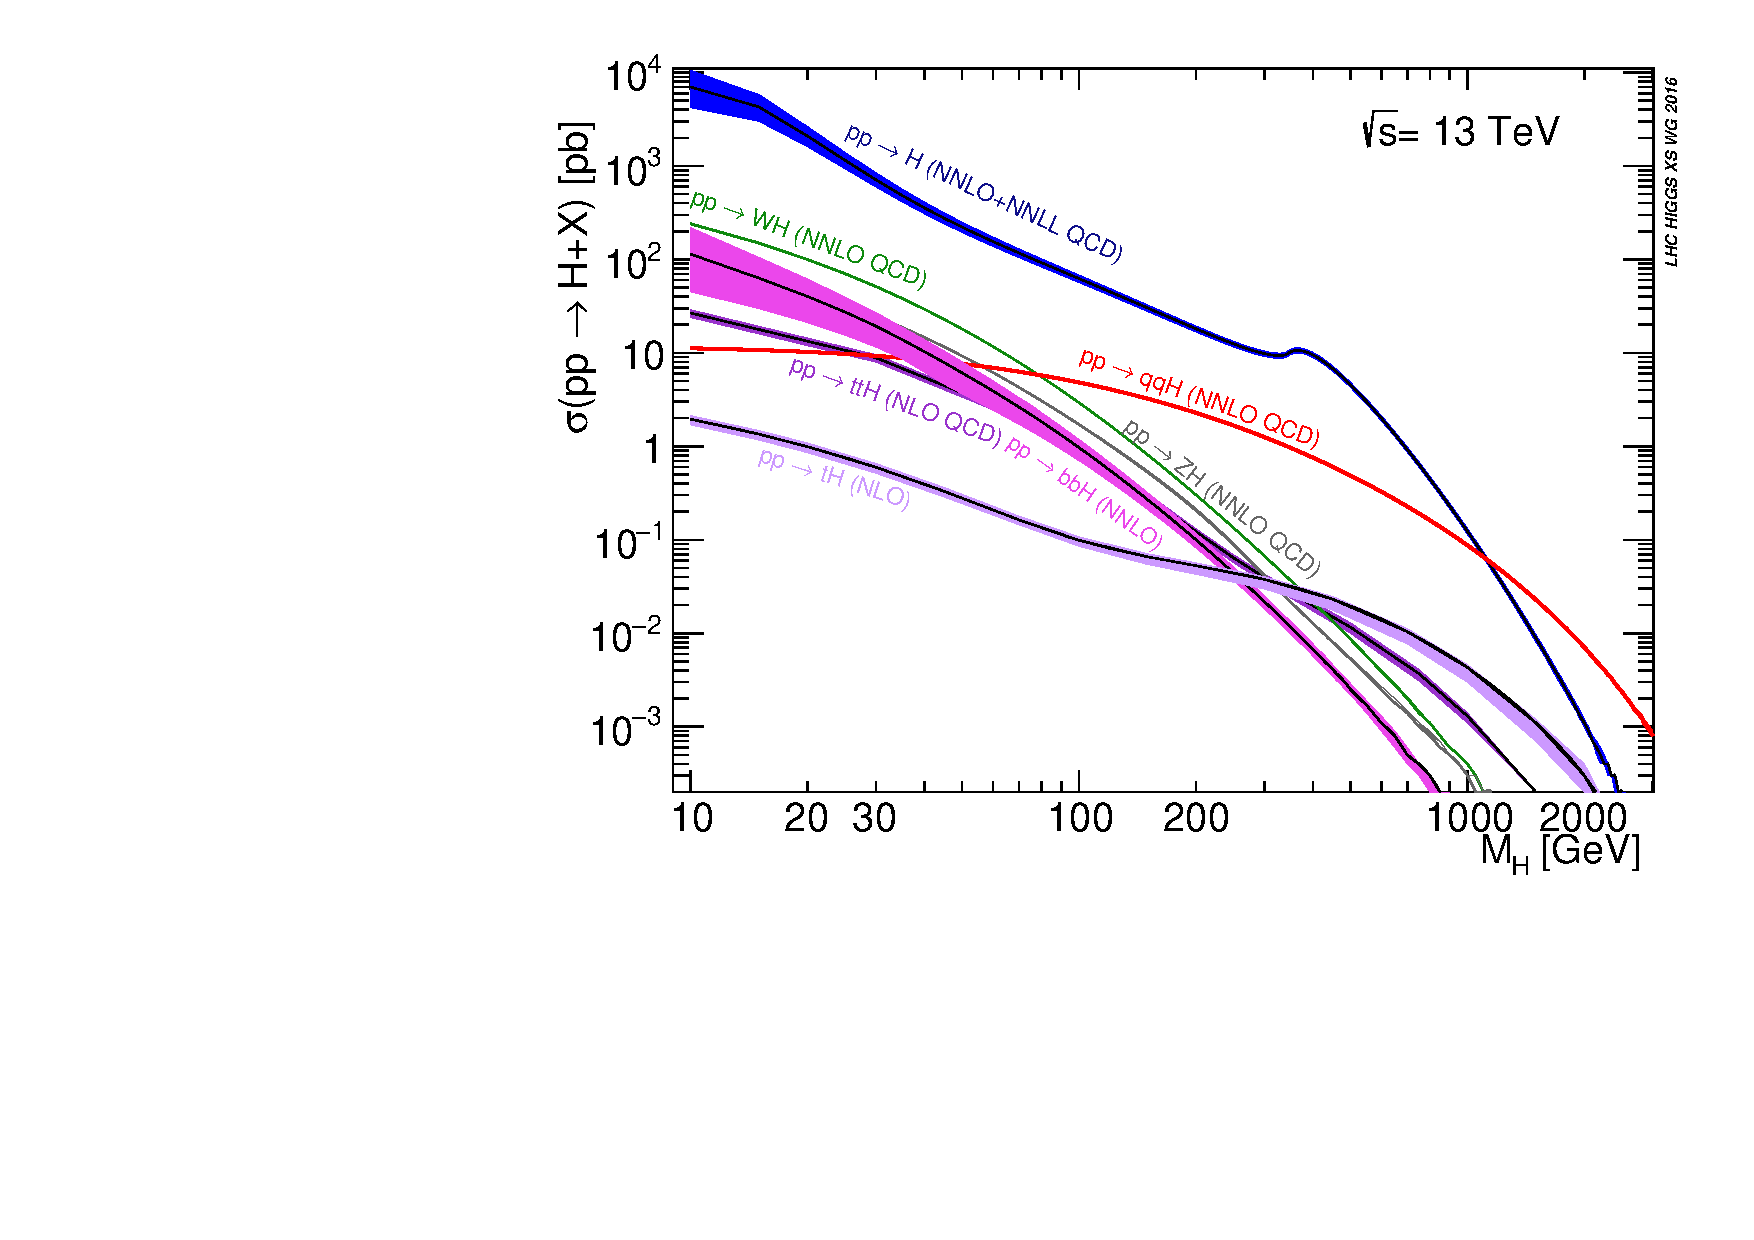
\includegraphics[width=0.45\textwidth]{figures/plotAll_13tev_BSM_sqrt}}
{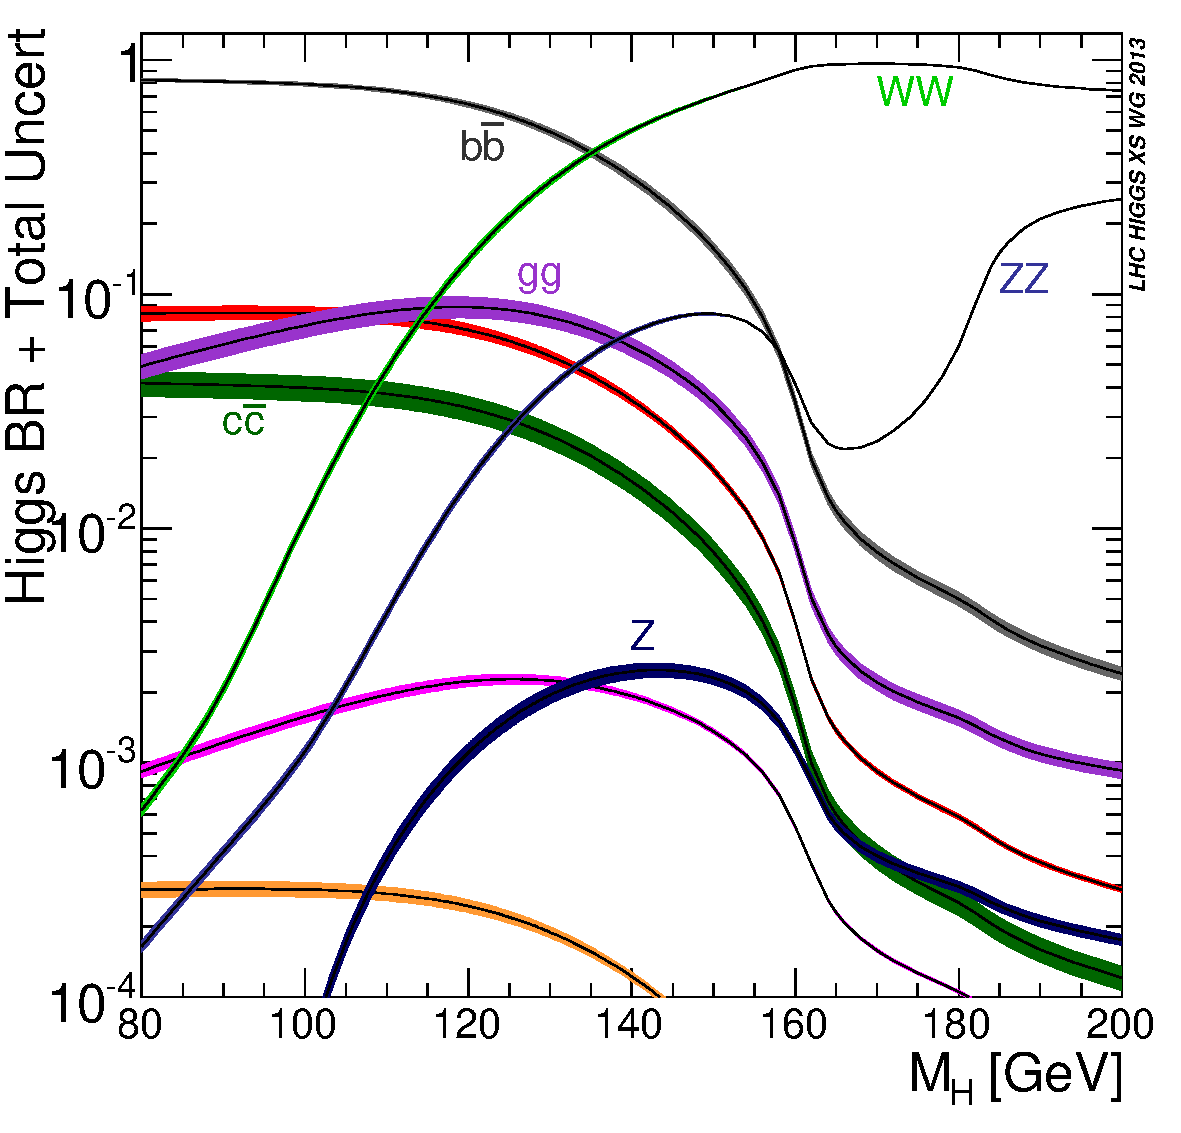
\includegraphics[width=0.4\textwidth]{figures/Higgs_BR_LM}}
\caption{ (Left) The Higgs production cross section, as a function of the Higgs boson mass, for proton-proton colliders at 13 TeV. (Right) The Higgs branching fractions to SM particles, as a function of the Higgs boson mass. }
\label{fig:hig_br_xsec}      
\end{figure}    


Even though the Higgs boson only directly couples to massive particles, processes via loops allow decays such as $H\rightarrow\gamma\gamma$ and production mechanisms such as $gg\rightarrow H$, where $g$ are gluons. 
The latter example is particularly important, since it is the production mechanism with highest cross section at the Large Hadron Collider, a proton-proton collider. 
For other types of colliders, this picture might be different, such as for the Tevatron (proton-antiproton), in which the main production mechanism was through associated production with an electroweak boson. 


\section{Higgs Physics Current Status}

While the Higgs boson, and the electroweak symmetry breaking mechanism applied to the SM itself, was predicted in the 60s, it wasn't until 2012 that it was experimentally verified. 
The CMS and ATLAS experiments, working at the Large Hadron Collider at CERN, detected statistically significant signals compatible with the SM predictions for the Higgs boson, using approximately 5 fb$^{-1}$ of 7 TeV and 8 TeV data \cite{higgs_cms, higgs_atlas}. 

In 2012, it was not possible to say with certainty that this anomaly was, without a doubt, the SM Higgs. 
However, five years later, the data that has been analyzed by the LHC experiments has confirmed the SM predictions for this new particle, with a mass measured as about $125$ GeV, including its spin (scalar) and CP eigenvalue (even) \cite{spin_cms, spin_atlas}. 

The Higgs boson decays to electroweak bosons, $H\rightarrow WW$, $H\rightarrow ZZ$ and $H\rightarrow \gamma\gamma$, have been measured and these branching fractions, assuming SM-like cross section, match the expected values. 
The Higgs decay modes to pairs of fermions have yet to be detected with the statistical significance seen in its bosonic modes. 
However, decays involving the third generation of quarks and leptons, $H\rightarrow b\bar{b}$ and $H\rightarrow \tau\tau$, have seen evidence of such processes when combining searches in different production channels. 
The latest results summary published by CMS and ATLAS can bee seen in Figure \ref{fig:hig_run1_summary} in terms of signal strengths ($\mu$), defined as the ratio of the measured Higgs boson rate to its SM prediction \cite{higgs_pros_cms_atlas}.

\begin{figure}[H]        
\centering                
{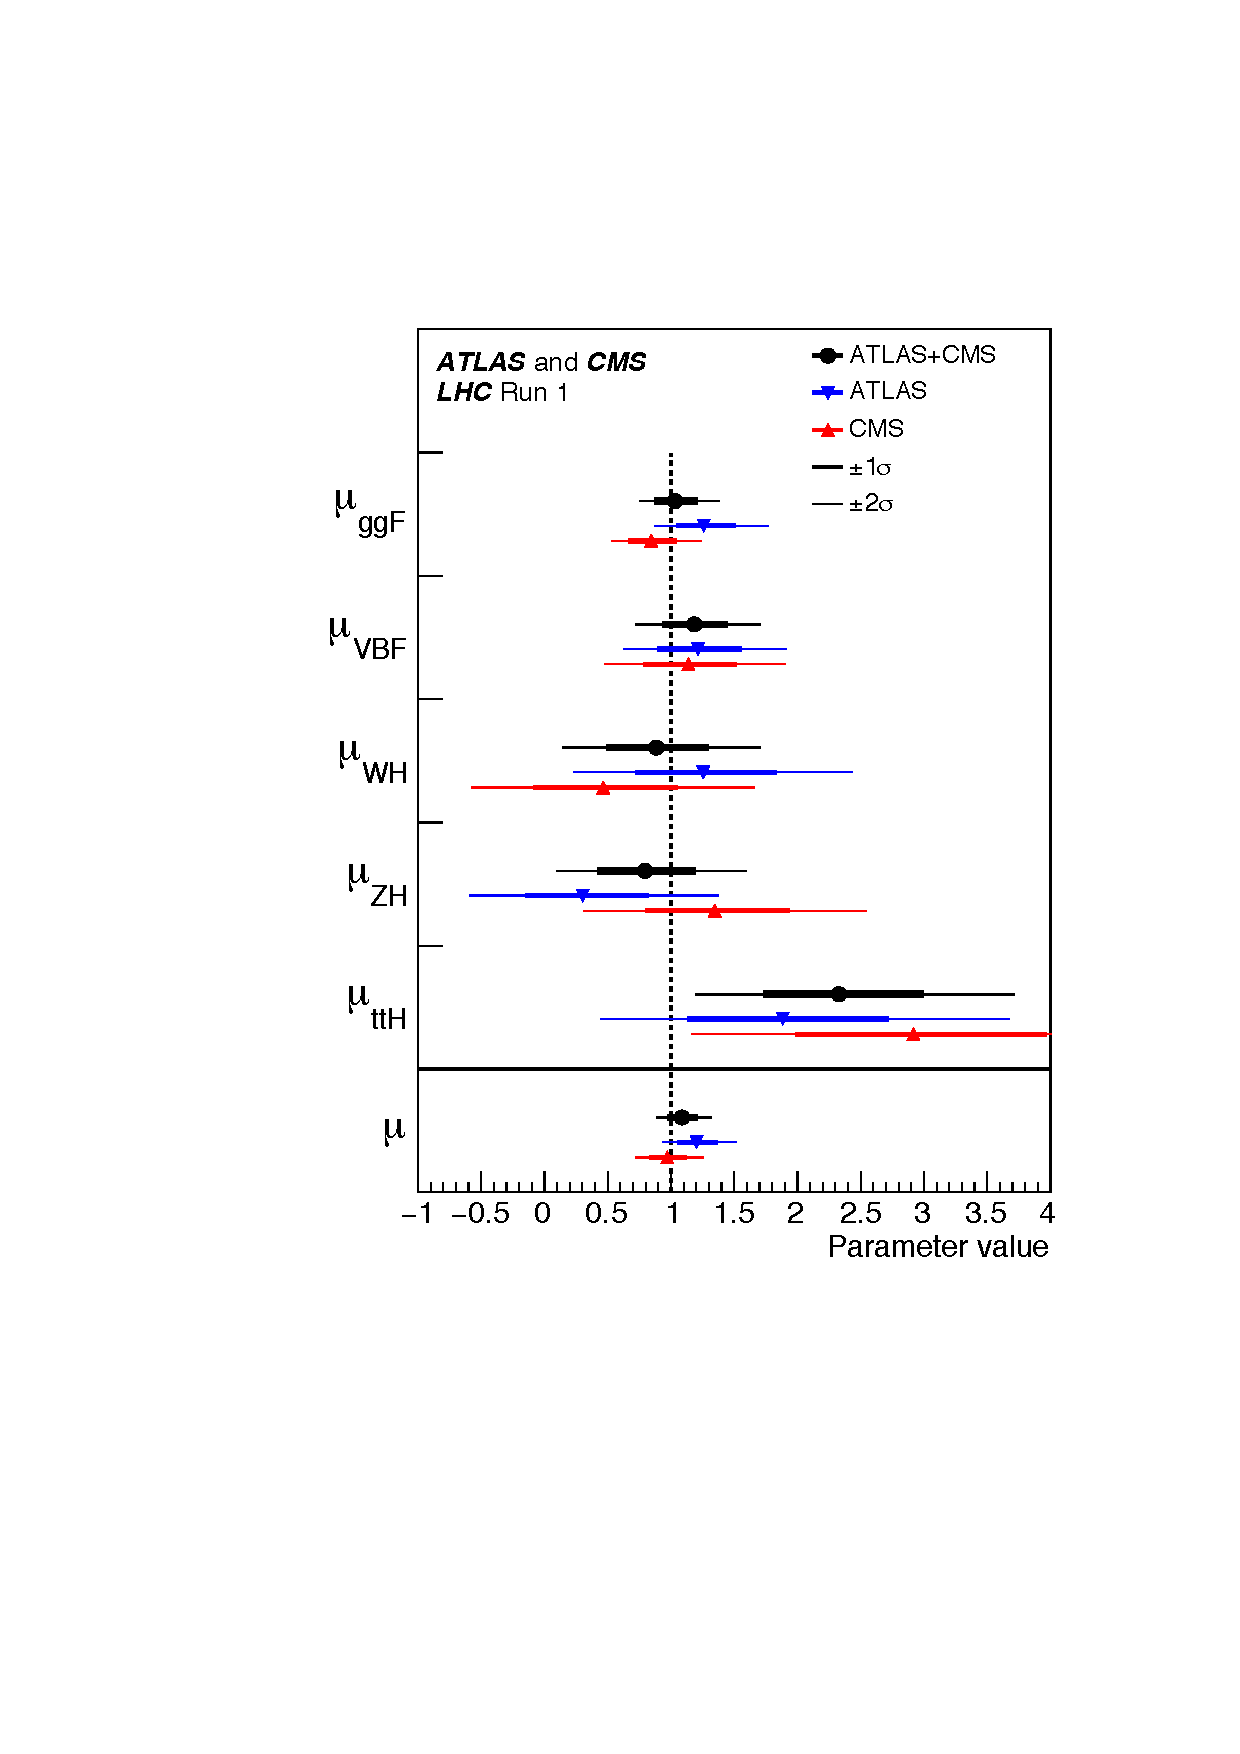
\includegraphics[width=0.45\textwidth]{figures/higgs_prod_run1}}
{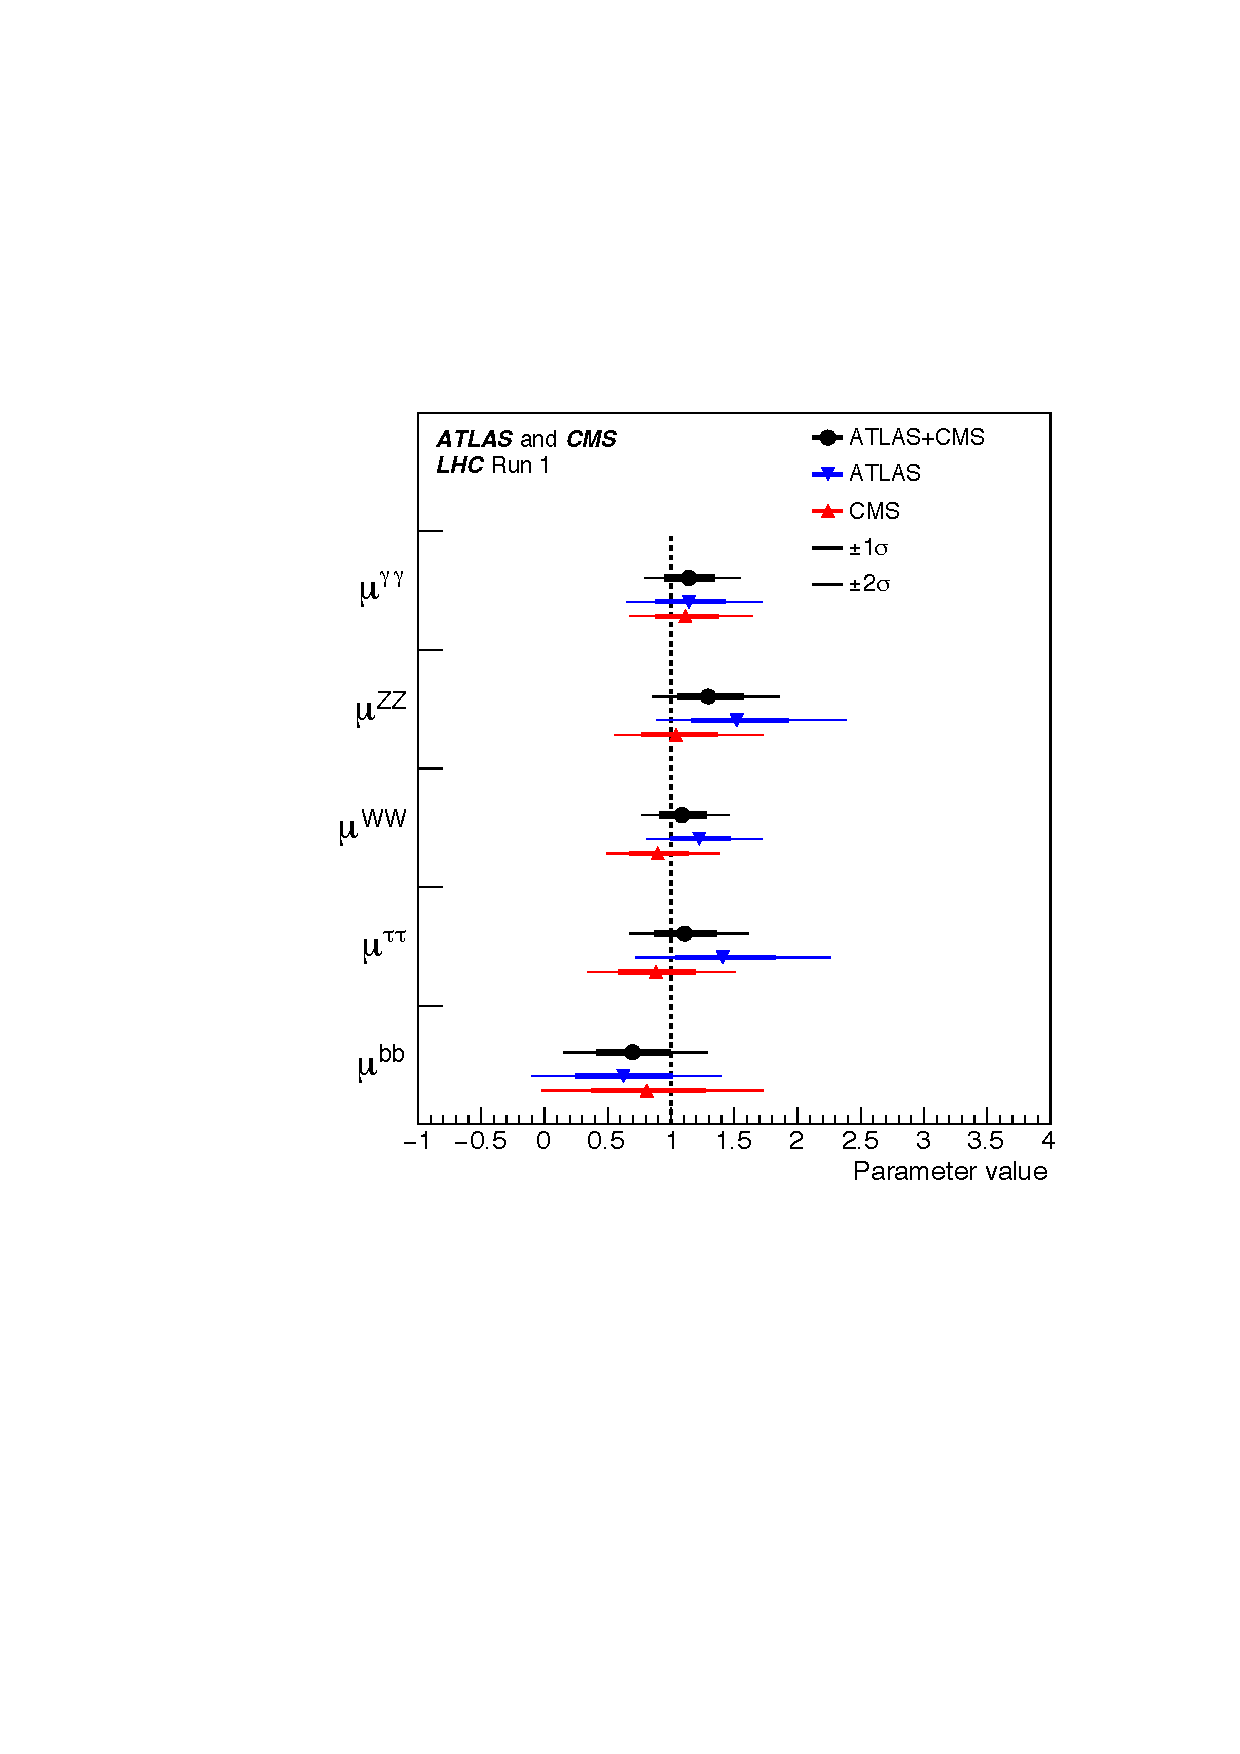
\includegraphics[width=0.45\textwidth]{figures/higgs_decay_run1}}
\caption{ (Left) The signal strength measured for the five main Higgs boson production mechanisms, assuming SM branching fractions. (Right) The signal strength measured for the three bosonic Higgs decays and the two third family fermionic decays, assuming SM production. }
\label{fig:hig_run1_summary}      
\end{figure}    

Other than measuring signal strengths, an important part of studying the Higgs boson is understanding its differential properties. 
Measuring kinematic distributions related to the Higgs candidates, such as the transverse momentum and pseudo-rapidity profiles, can indicate possible corrections and beyond the SM contributions to the production mechanisms. 
For example, new particles appearing in the gluon fusion loop can have different coupling structures that induce kinematic correlations not present in the SM. 
In Figure \ref{fig:hig_diff}, the CMS differential Higgs boson measurements using the $H\rightarrow\gamma\gamma$ channel in terms of the Higgs transverse momentum and rapidity using 8 TeV data \cite{higgs_diff}. 


\begin{figure}[H]        
\centering                
{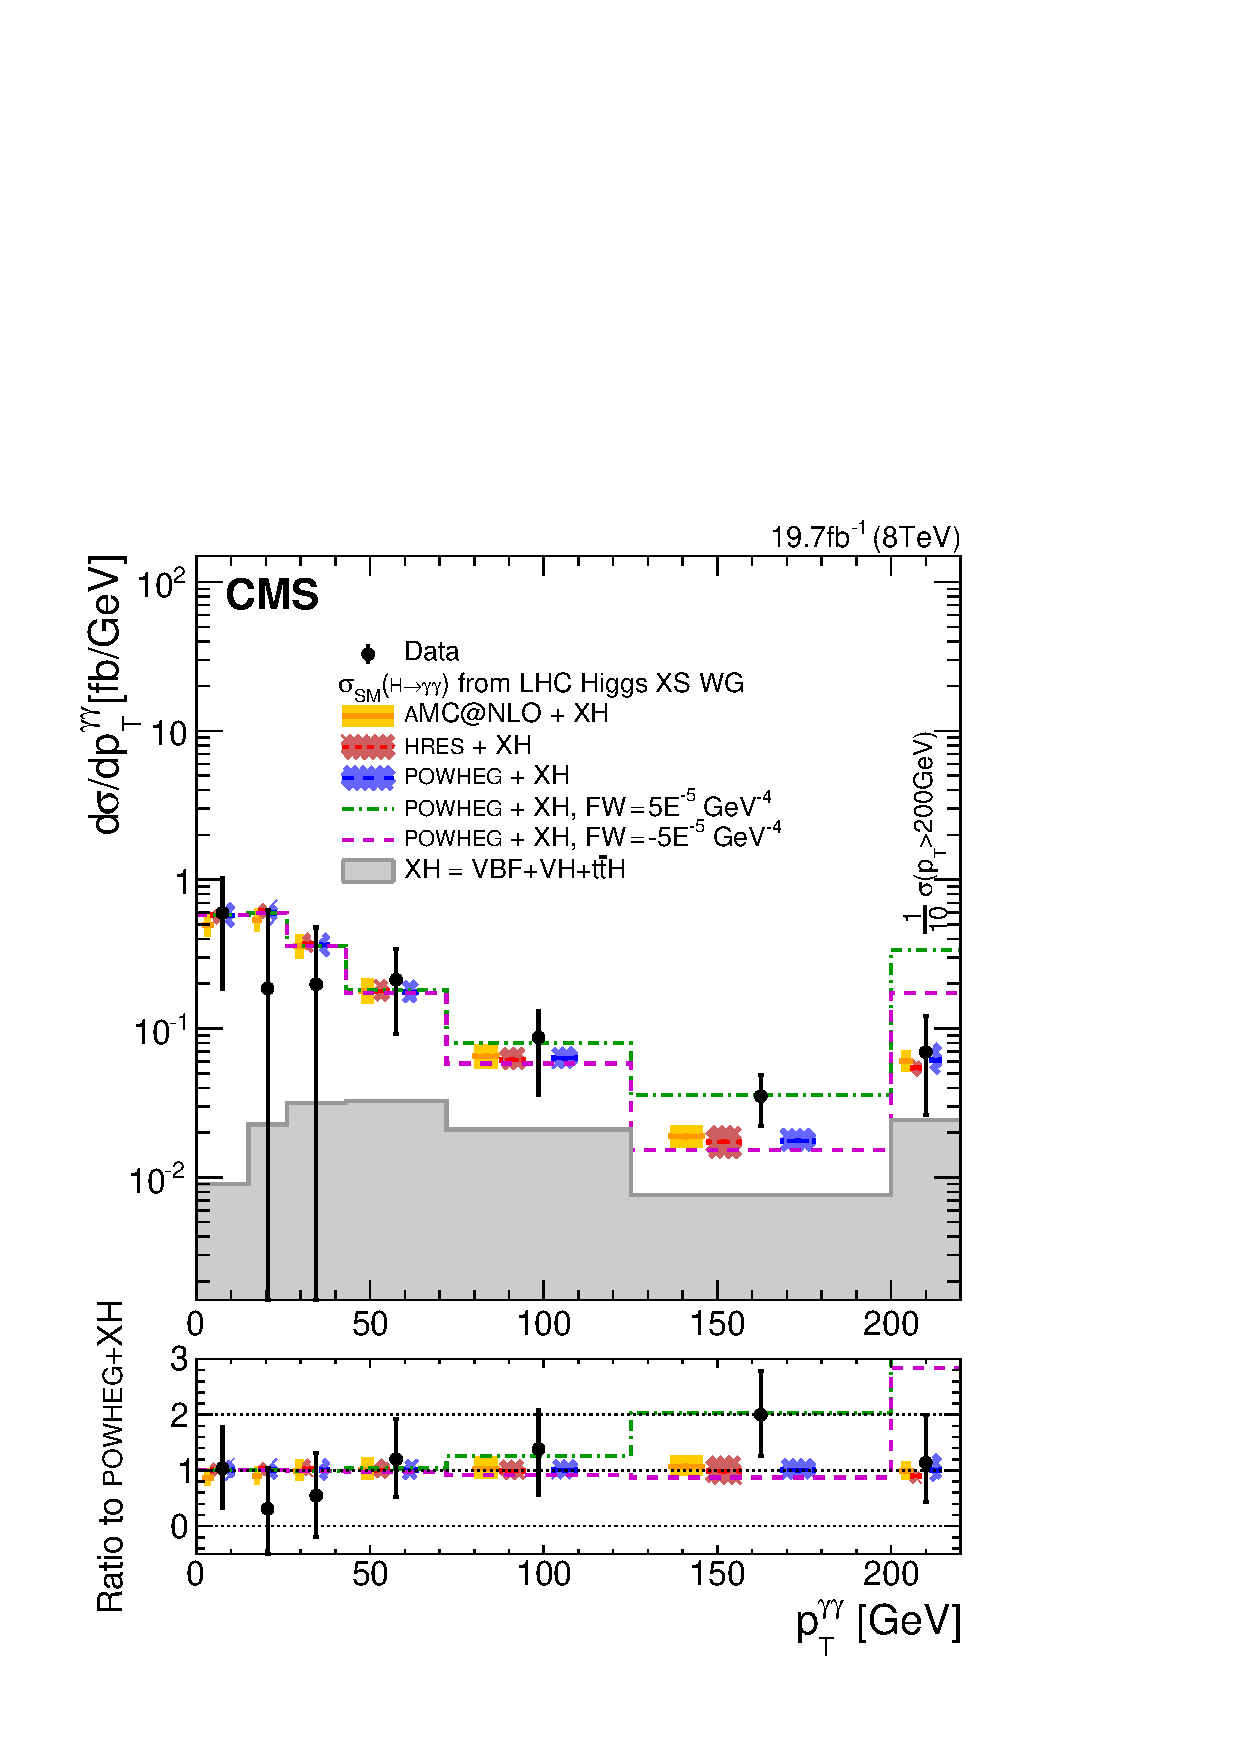
\includegraphics[width=0.45\textwidth]{figures/higgs_diff_pt}}
{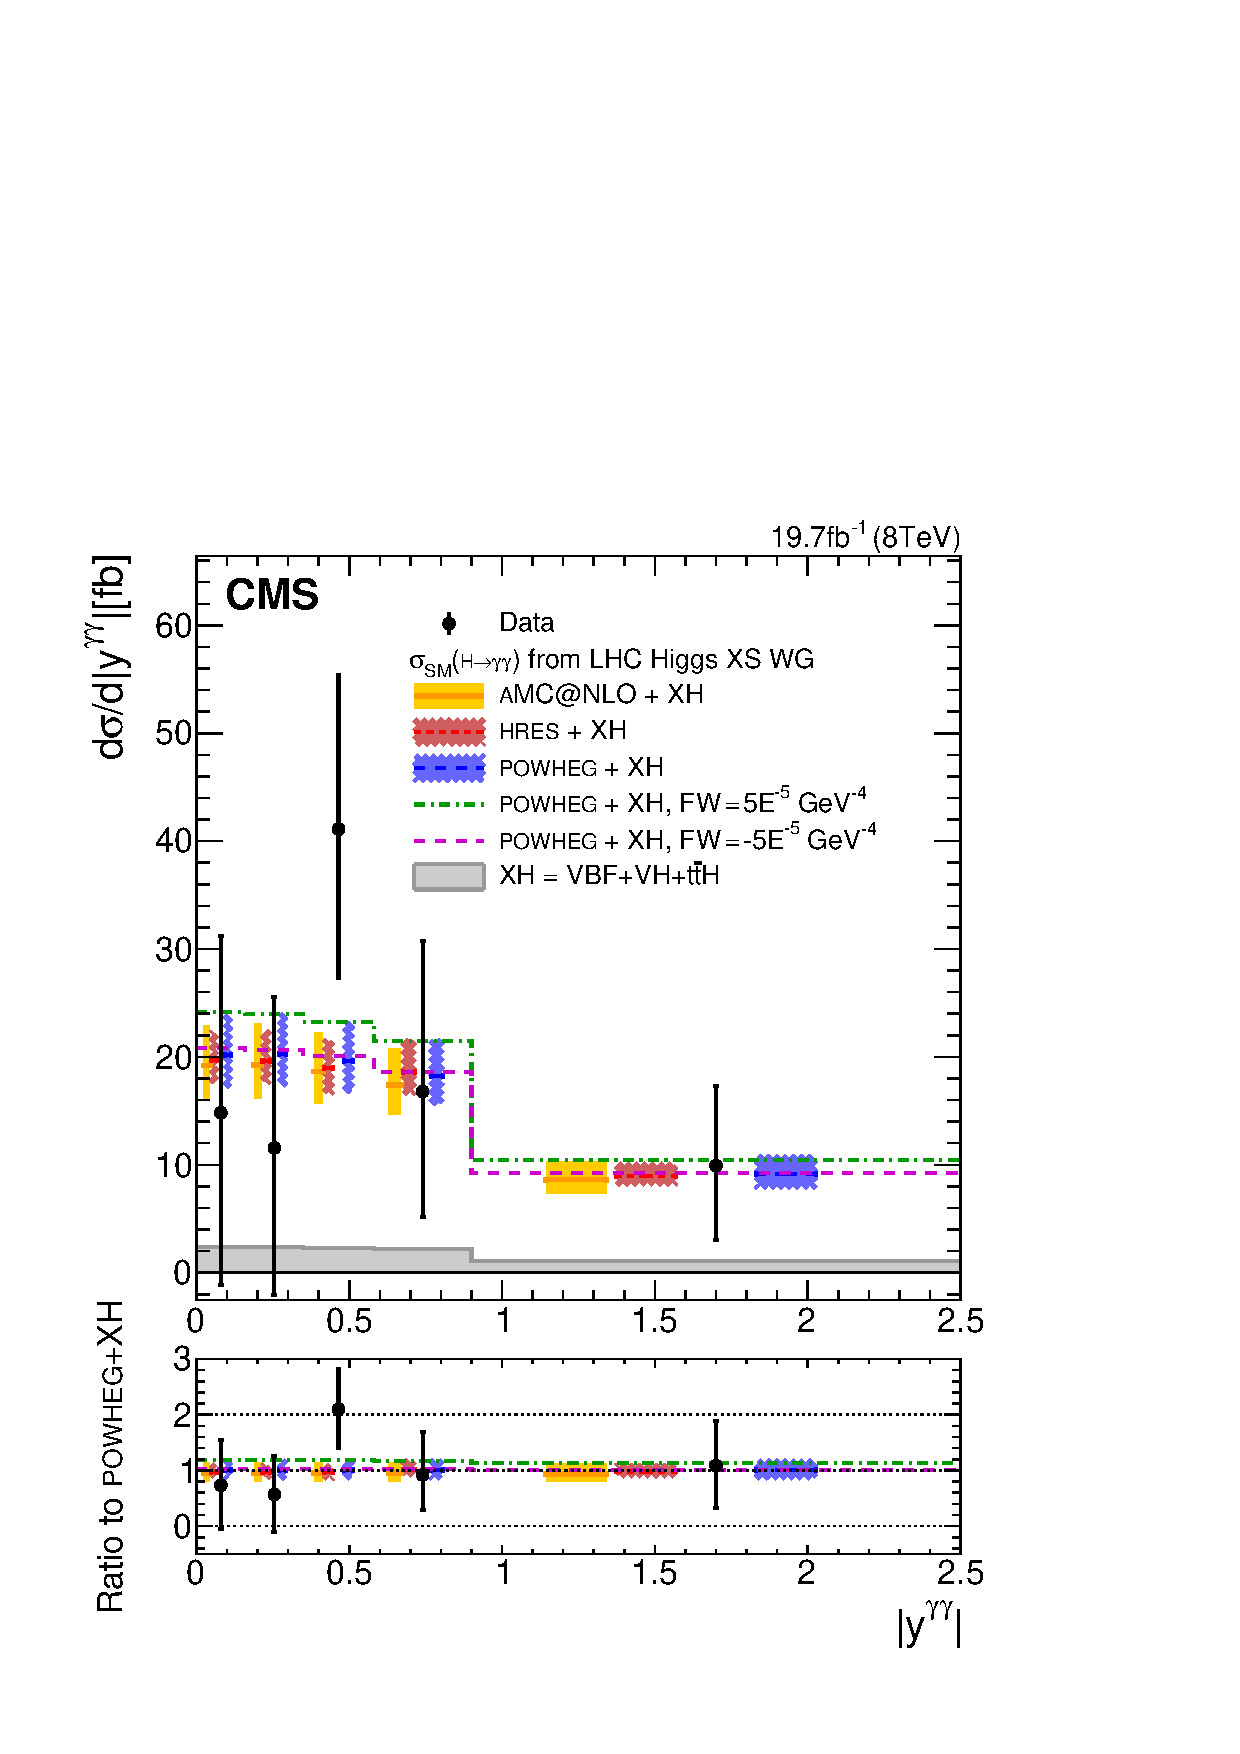
\includegraphics[width=0.45\textwidth]{figures/higgs_diff_rap}}
\caption{ CMS differential Higgs boson measurements using the $H\rightarrow\gamma\gamma$ channel in terms of the Higgs transverse momentum (left) and rapidity (right) using 8 TeV data. The measurements are compared to different Monte Carlo generators. }
\label{fig:hig_diff}      
\end{figure}    



\section{Higgs as a Probe of New Physics}

The experimental confirmation of the Higgs boson marks another success of the SM. 
However, the measured mass of the Higgs boson poses a naturalness conundrum: being a scalar, the Higgs mass is subject to higher order corrections from loops that contain spin 0, 1/2 and 1 particles, which diverge as a function os the energy scale.  
If the SM is valid for all energy scales, these corrections would take the Higgs mass to its highest possible energy scale, the Planck scale ($\approx 10^{19}$ GeV), which is in clear contrast with the Higgs mass value known today. 
In principle, it is possible that the higher order corrections to the Higgs mass cancel out in a way to leave $m_{H} = 125$ GeV, however, such an "accidental" fine tuning is not well motivated within the theory. 
The presence of these two distinct and far apart energy scales in the electroweak theory (Higgs mass and electroweak vacuum versus the Planck scale) is called the Hierarchy problem. 

Several models and extensions to the SM have been proposed to solve the Hierarchy problem. 
Among them, and perhaps the most famous, is Supersymmetry (SUSY) \cite{GGMa,GGMd2,GGMd3,GGMd4,GGMd5,GGMd1,GGMd}. 
SUSY explains the higher order cancelations by postulating a new symmetry of nature that correlates bosons and fermions. 
By symmetrizing the bosonic and fermionic contributions to the Higgs mass corrections, the higher order terms are canceled out naturally (since fermion loops contribute with an overall minus sign relative to boson loops). 

The existence of SUSY implies that, for every elementary fermion in nature, there must exist a boson superpartner with the same mass (same applies to bosons and fermion superpartners). 
However, this has not been observed, which means that, if SUSY exists, it must be a broken symmetry. 
In order to still address the Hierarchy problem, the SUSY breaking scale must be such that the superpartner masses should not exceed $\mathcal{O}(1$ TeV$)$. 
This requirement also has the feature that it unifies the QCD and electroweak coupling constants at $\mathcal{O}(10^{16}$ GeV$)$.

The simplest supersymmetric extension of the SM, known as the Minimal Supersymmetric SM (MSSM), adds the minimal amount of extra fields to the current model to realized SUSY - in the MSSM, each SM fermion/boson will have one boson/fermion superpartner. 
It also introduces changes to the Higgs sector: two Higgs doublets are required in order to perform the electroweak symmetry breaking, and give masses to both up and down type quarks and leptons. 
The existence of this extra doublet now implies that, instead of one Higgs boson mass state, five new bosons exist: two neutral CP-even bosons: $h$, $H$ (one of which is usually identified as the particle discovered in 2012); one neutral CP-odd boson (pseudoscalar): $A$; and two charged charged bosons: $H^{\pm}$. 

The MSSM is one example of model that adds to the Higgs sector of the SM an extra scalar doublet. 
Models with this characteristic are generally referred as Two-Higgs Doublet Models (2HDM) \cite{2hdm}. 
These models are also characterized by new phenomena related to the SM-like Higgs boson, either by exotic production or decay. 
For the first case to happen, at least one of the new resonances in the model, $H$ for example, must be heavier than the SM-like Higgs ($h$), which then allows decays such as $H\rightarrow h+X$, where $X$ can either be a $Z$, an $A$ or even another $h$. 
Alternatively, if $A$, for example, is lighter than $m_{h}/2 \approx 62.5$ GeV, decays such as $h\rightarrow AA$ become possible. 

These specific models serve as illustrations of how a modification to the SM can lead to exotic physics to appear in the Higgs sector. 
More generally, looking for new physics with the Higgs boson is a justifiable ansatz in both phenomenological terms - most extensions to the SM predict specific modifications of the Higgs sector - and in theoretical terms - the Higgs sector is intimately tied to some of the most undesirable features of the SM, such as the Hierarchy problem. 
Another one of these undesirable features is the electroweak vacuum stability problem.

The electroweak vacuum in the SM is defined as the vacuum expectation value given by the Higgs potential minimum: $v \approx 246$ GeV. 
Even though the Higgs potential has one global minimum associated to this vacuum, higher order corrections change the shape of this potential and can turn this global minimum into a local minimum. 
The impact of these corrections are mostly dominated by the Higgs-top quark Yukawa coupling, and so, the stability of the electroweak vacuum depends on the Higgs mass and on the top quark mass, as seen in Figure \ref{fig:hig_stab} \cite{vacuum_stab}. 

Given the current values for the Higgs boson and the top quark masses, our universe currently lies at a meta-stable point. 
These instabilities in the electroweak vacuum can have catastrophic consequences to the fate of the universe, since the vector boson masses, and therefore the strength of the weak interactions, are tied to this value. 
If it is indeed confirmed that we live in such a state, with more precise measurements for the mass parameters, new mechanisms must be in place to safeguard the universe against these features.


 \begin{figure}[h]        
\centering                
{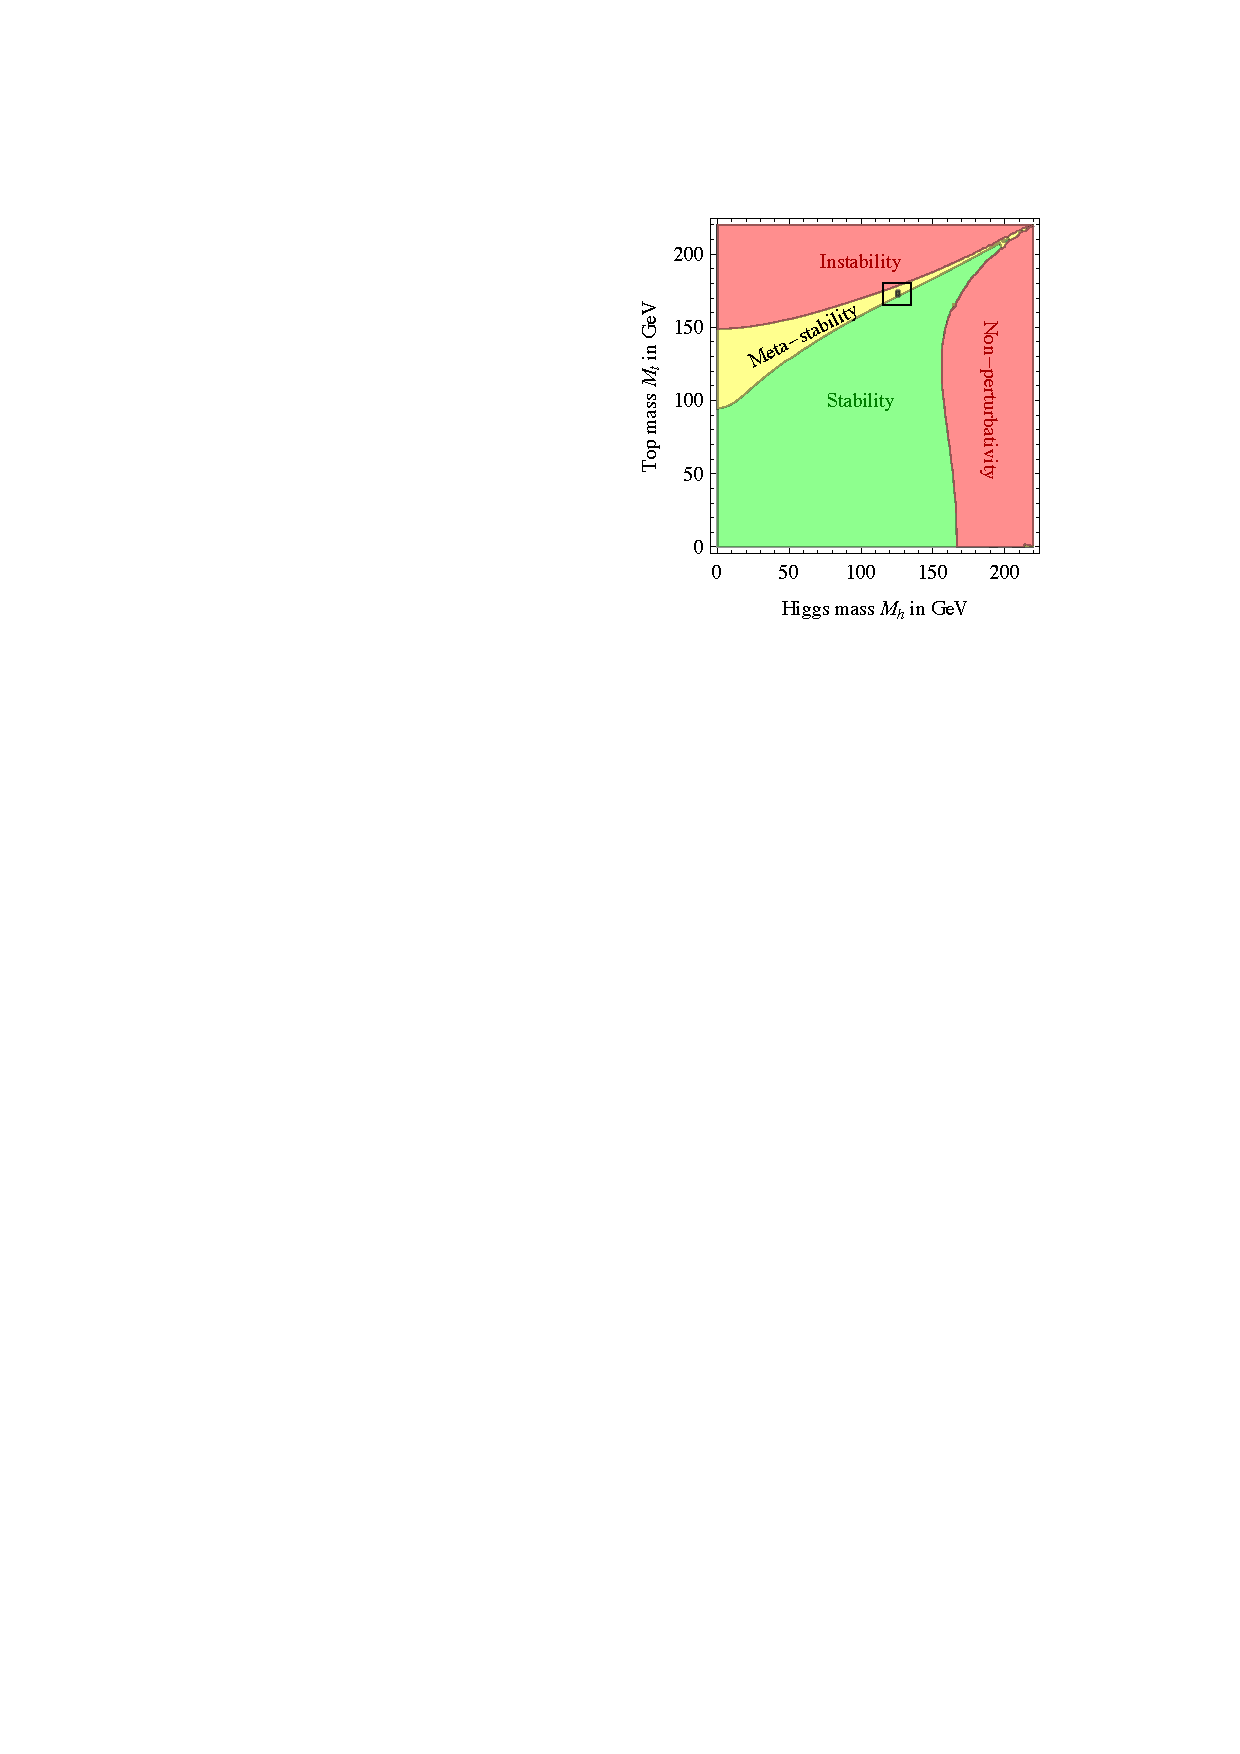
\includegraphics[align=c,width=0.45\textwidth]{figures/higgs_vac_stab}}
{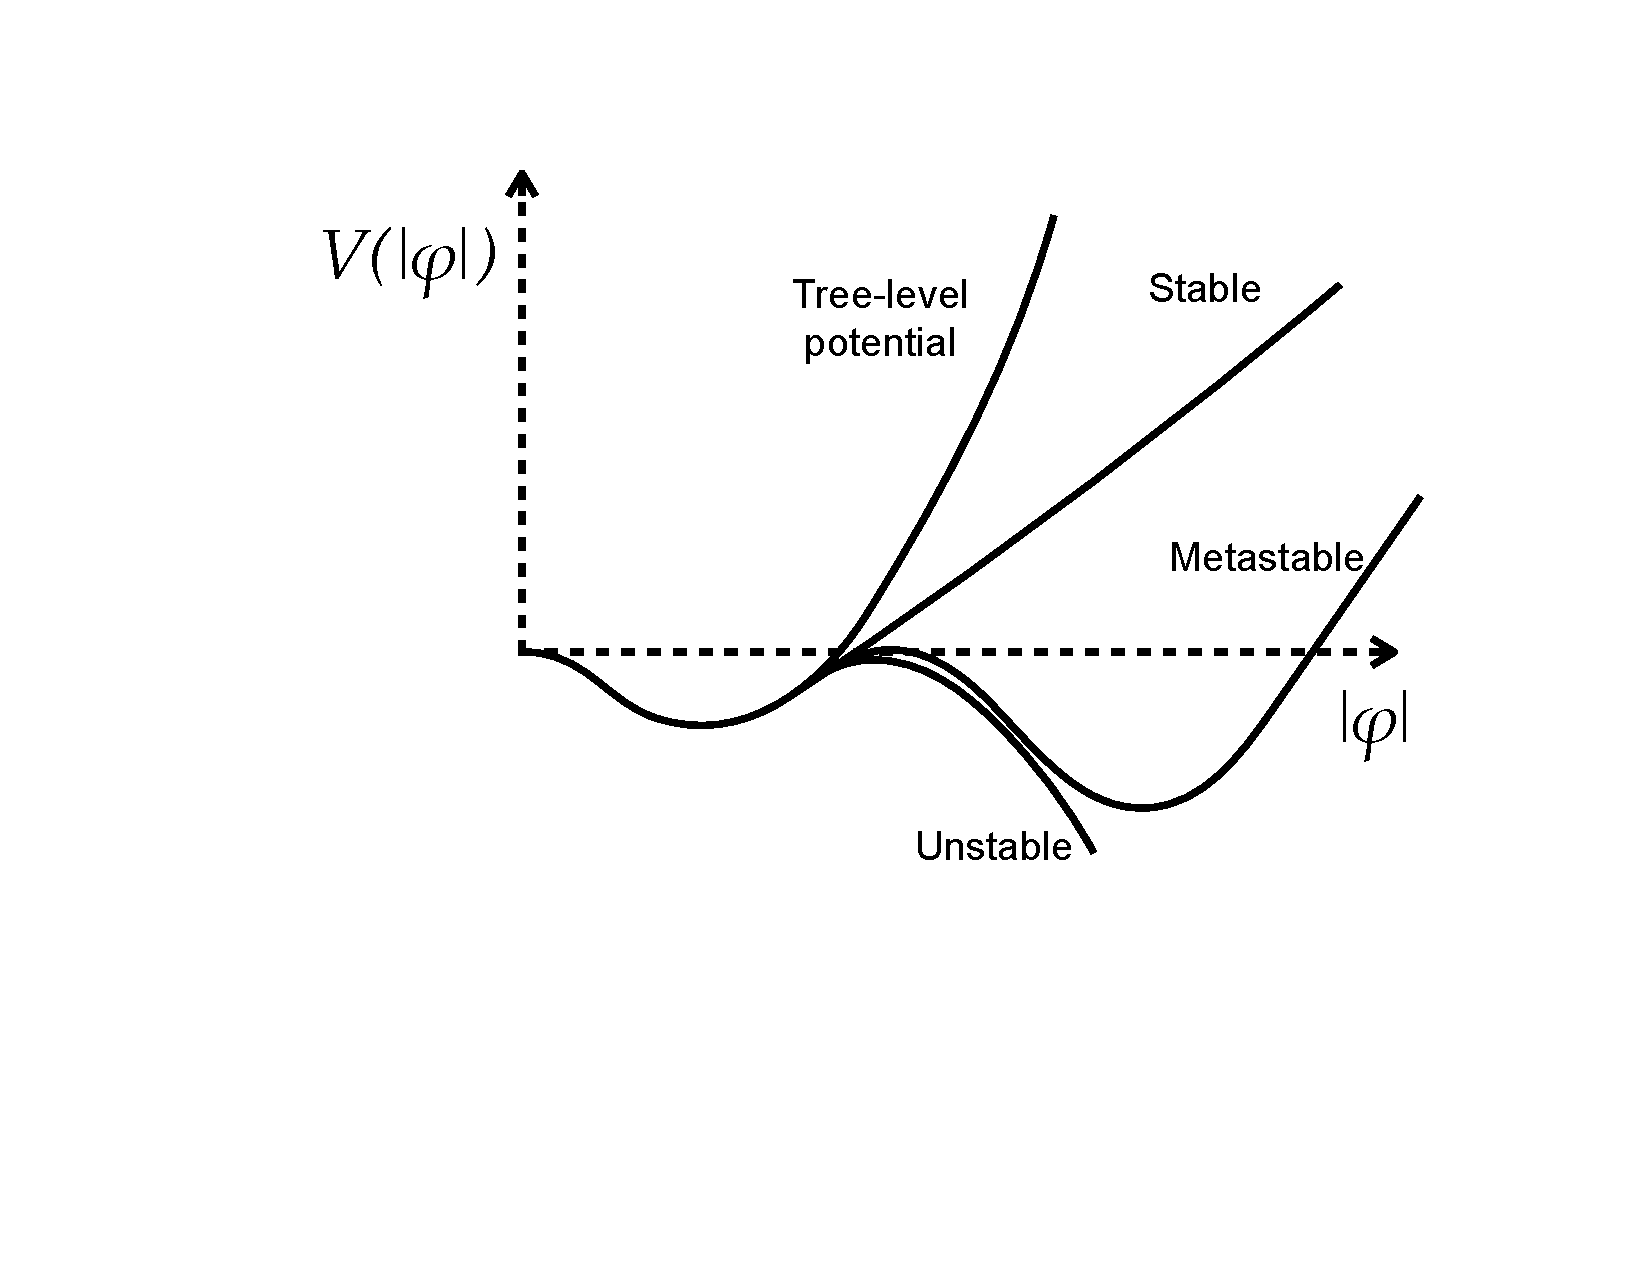
\includegraphics[align=c,width=0.45\textwidth]{figures/higgs_pot_mod}}
\caption{ CMS differential Higgs boson measurements using the $H\rightarrow\gamma\gamma$ channel in terms of the Higgs transverse momentum (left) and rapidity (right) using 8 TeV data. The measurements are compared to different Monte Carlo generators. }
\label{fig:hig_stab}      
\end{figure}    

One important caveat of this stability analysis is the assumption that the tree-level Higgs potential has the quartic shape described in Equation \ref{eq:higgs_pot}. 
However, there are no strong theoretical indications that $V(|\Phi|)$ must have this exact shape. 
Theoretically, the SM $V(|\Phi|)$ is the simplest potential that correctly breaks the electroweak symmetry within theoretical constraints, such as unitarity and renormalizability. 

Experimentally, in order to probe its shape, the $V(|\Phi|)$ potential parameters must be measured directly. 
Through the detection of the Higgs boson and its mass measurement, the parameter $\mu$ in $V(|\Phi|)$ is determined, since $m_{h} = |\mu|$. 
As seen in Equation \ref{eq:higgs_pot_aberto}, the higher order terms of $V(|\Phi|)$ are related to Higgs self-interaction terms. 
It's important to note that, even if the \textit{true} Higgs potential (the one that correctly breaks the electroweak symmetry and brings stability to the SM) is not $V(|\Phi|)$, an expansion of this general potential around the vacuum will generally create higher order terms with respect to $H$. 
Therefore, directly measuring the Higgs self-interaction terms, such as the Higgs triple coupling, is a crucial step towards understanding the SM.





\chapter{The Compact Muon Solenoid Experiment at the Large Hadron Collider}
\graphicspath{{cms/figures/}{cms/}}

The Compact Muon Solenoid (CMS) experiment is one of the four experiments operating at the Large Hadron Collider (LHC) particle accelerator at the European Center for Nuclear Research (CERN), in the suburbs of Geneva, Switzerland. 
Along with ATLAS, LHCb and ALICE, they are the latest generation of high energy physics experiments to take place at colliders. 
CMS and ATLAS are multi-purpose experiments, looking for different types of processes coming from the proton-proton collisions at the LHC, while LHCb and ALICE are designed for specific purposes: rare processes involving flavor physics and QCD at high temperatures, respectively.  
In the following sections, the LHC will be briefly summarized, followed by a description of the CMS experiment.

\section{The LHC Accelerator Complex}

The Large Hadron Collider (LHC) is a circular hadron-hadron collider operated at European Organization for Nuclear Research (CERN) in Geneva, Switzerland. 
The collider has a circumference of 27 km and it is located in the underground tunnel that hosted the Large Electron Positron (LEP) collider, operated from 1989 until 2000. 
The LHC ring includes two adjacent beam pipes, each containing one of two colliding beams, which travel in opposite directions in the collider ring. 
The main part of the LHC physics program consists in operating the machine as a proton-proton (pp) collider, while part of the machine schedule is periodically dedicated to the delivery of heavy-ion collisions. 
The LHC ring includes two adjacent beam pipes, each containing one of two colliding beams, which travel in opposite directions. 
The two beams are focused and bent in their circular trajectory by a system of more than 1600 superconducting magnets: 
1232 dipole magnets operating at a temperature of less than 2 K generate a magnetic field of 8.3 T that maintains the circular motion of the two beams around the LHC; 
392 quadrupole magnets are used to keep the beams focused as they travel inside the collider. 

In the LHC, beams are accelerated by the electromagnetic field generated by radio-frequency cavities (eight per beam) located along the collider ring. 
Each of these cavities also operates in superconducting state, at a temperature of approximately 4.5 K, and can deliver a voltage of 2 MV at a frequency of 400 MHz. 
Prior to their injection in the LHC, the colliding particles (protons or heavy-ions) are grouped together in bunches and pre-accelerated in a chained system of smaller accelerators, which complete the CERN accelerator complex. 
A layout of the CERN accelerator complex can be seen in Figure \ref{fig:lhc}.

\begin{figure*}[h]
\centering 
\includegraphics[width=0.99\textwidth]{figures/lhc}\hfil
\caption{Sketch of the CERN accelerator complex, including the Large Hadron Collider. }
\label{fig:lhc}
\end{figure*}

The LHC was designed to deliver pp collisions at a center of mass energy of $\sqrt{s} = 14$ TeV with an instantaneous luminosity of $10^{34}$ cm$^{-2}$s$^{-1}$, using a bunch-spacing of 25 ns. 
In the first years of data-taking, the LHC operated below the design values to reduce the time needed for commissioning the machine and to follow a safer strategy concerning the operation of the LHC magnets.
The first run of the LHC physics program with pp collisions started in 2009 at $\sqrt{s} = 7$ TeV and continued through 2010 and 2011 reaching a maximum instantaneous luminosity of $3.5 \times 10^{33}$ cm$^{-2}$s$^{-1}$ with a bunch spacing of 50 ns, translated into 5 fb$^{-1}$ collected by the CMS experiment. 
During 2012 and 2013, the center of mass energy was increased to $\sqrt{s} = 8$ TeV, and the machine reached a peak instantaneous luminosity of $7.7 \times 10^{33}$ cm$^{-2}$s$^{-1}$. 
In this period the CMS experiment recorded a total integrated luminosity of 19.7 fb$^{-1}$ with all subdetectors fully operational and nominal magnetic field.

From 2013 to 2015, the LHC went through upgrades aiming at operating the collider at its nominal configuration. 
The first stable collisions in 2015 were in May at $\sqrt{s} = 13$ TeV, with a bunch spacing of 50 ns, then changed to 25 ns later in the year, reaching a peak luminosity of $5 \times 10^{33}$ cm$^{-2}$s$^{-1}$. 
By the end of the first year of the LHC Run-2, the CMS experiment recorded a total integrated
luminosity of 2.6 fb$^{-1}$ with a magnetic field of 3.8 T and all subdetectors in full operation. 
The year of 2016 was a record breaking period for the LHC, with a peak luminosity of $1.4\times10^{34}$ cm$^{-2}$s$^{-1}$ (reaching its nominal value) and an integrated luminosity of about 40 fb$^{-1}$ in ATLAS and CMS. M

\section{The CMS Experiment}

The CMS experiment is one of the multi-purpose experiments at the LHC. 
Its goal is to measure both Standard Model processes and search for physics beyond the Standard Model. 
In order to achieve this, it must precisely reconstruct objects that are typically present at high energy colliders (photons, electrons, muons and hadronic jets), including their 4-momentum (3-dimensional momentum plus energy).  

The overall CMS design is that of a cylindrical onion, meaning that every individual subdetector (specializing in measuring different types of event information) is stacked together concentrically, like onion layers. 
These different subdetectors are shown in Figure \ref{fig:cms_sketch}, and will be described in the following sections. 

In order to measure charged particles momenta with the desired precision, a strong magnetic field must be present at the experiment, so the momentum can be extracted from the particles' bending. 
The CMS magnet is a superconducting solenoid located between the CMS calorimeters and muon detectors. 
It is 13 meters long, with 6 meters of inner diameter, and provides a 4T magnetic field. 
With this geometry, the direction of the magnetic field will be different at the CMS tracker system, in which charged particles trajectories are measured close to the interaction point, and at the CMS muon system, which is a tracking subdetector specialized in measuring muon trajectories. 
This optimizes the muon momentum measurement by having two magnetic bendings in the reconstructed muon path, instead of only one. 

\begin{figure*}[h]
\centering 
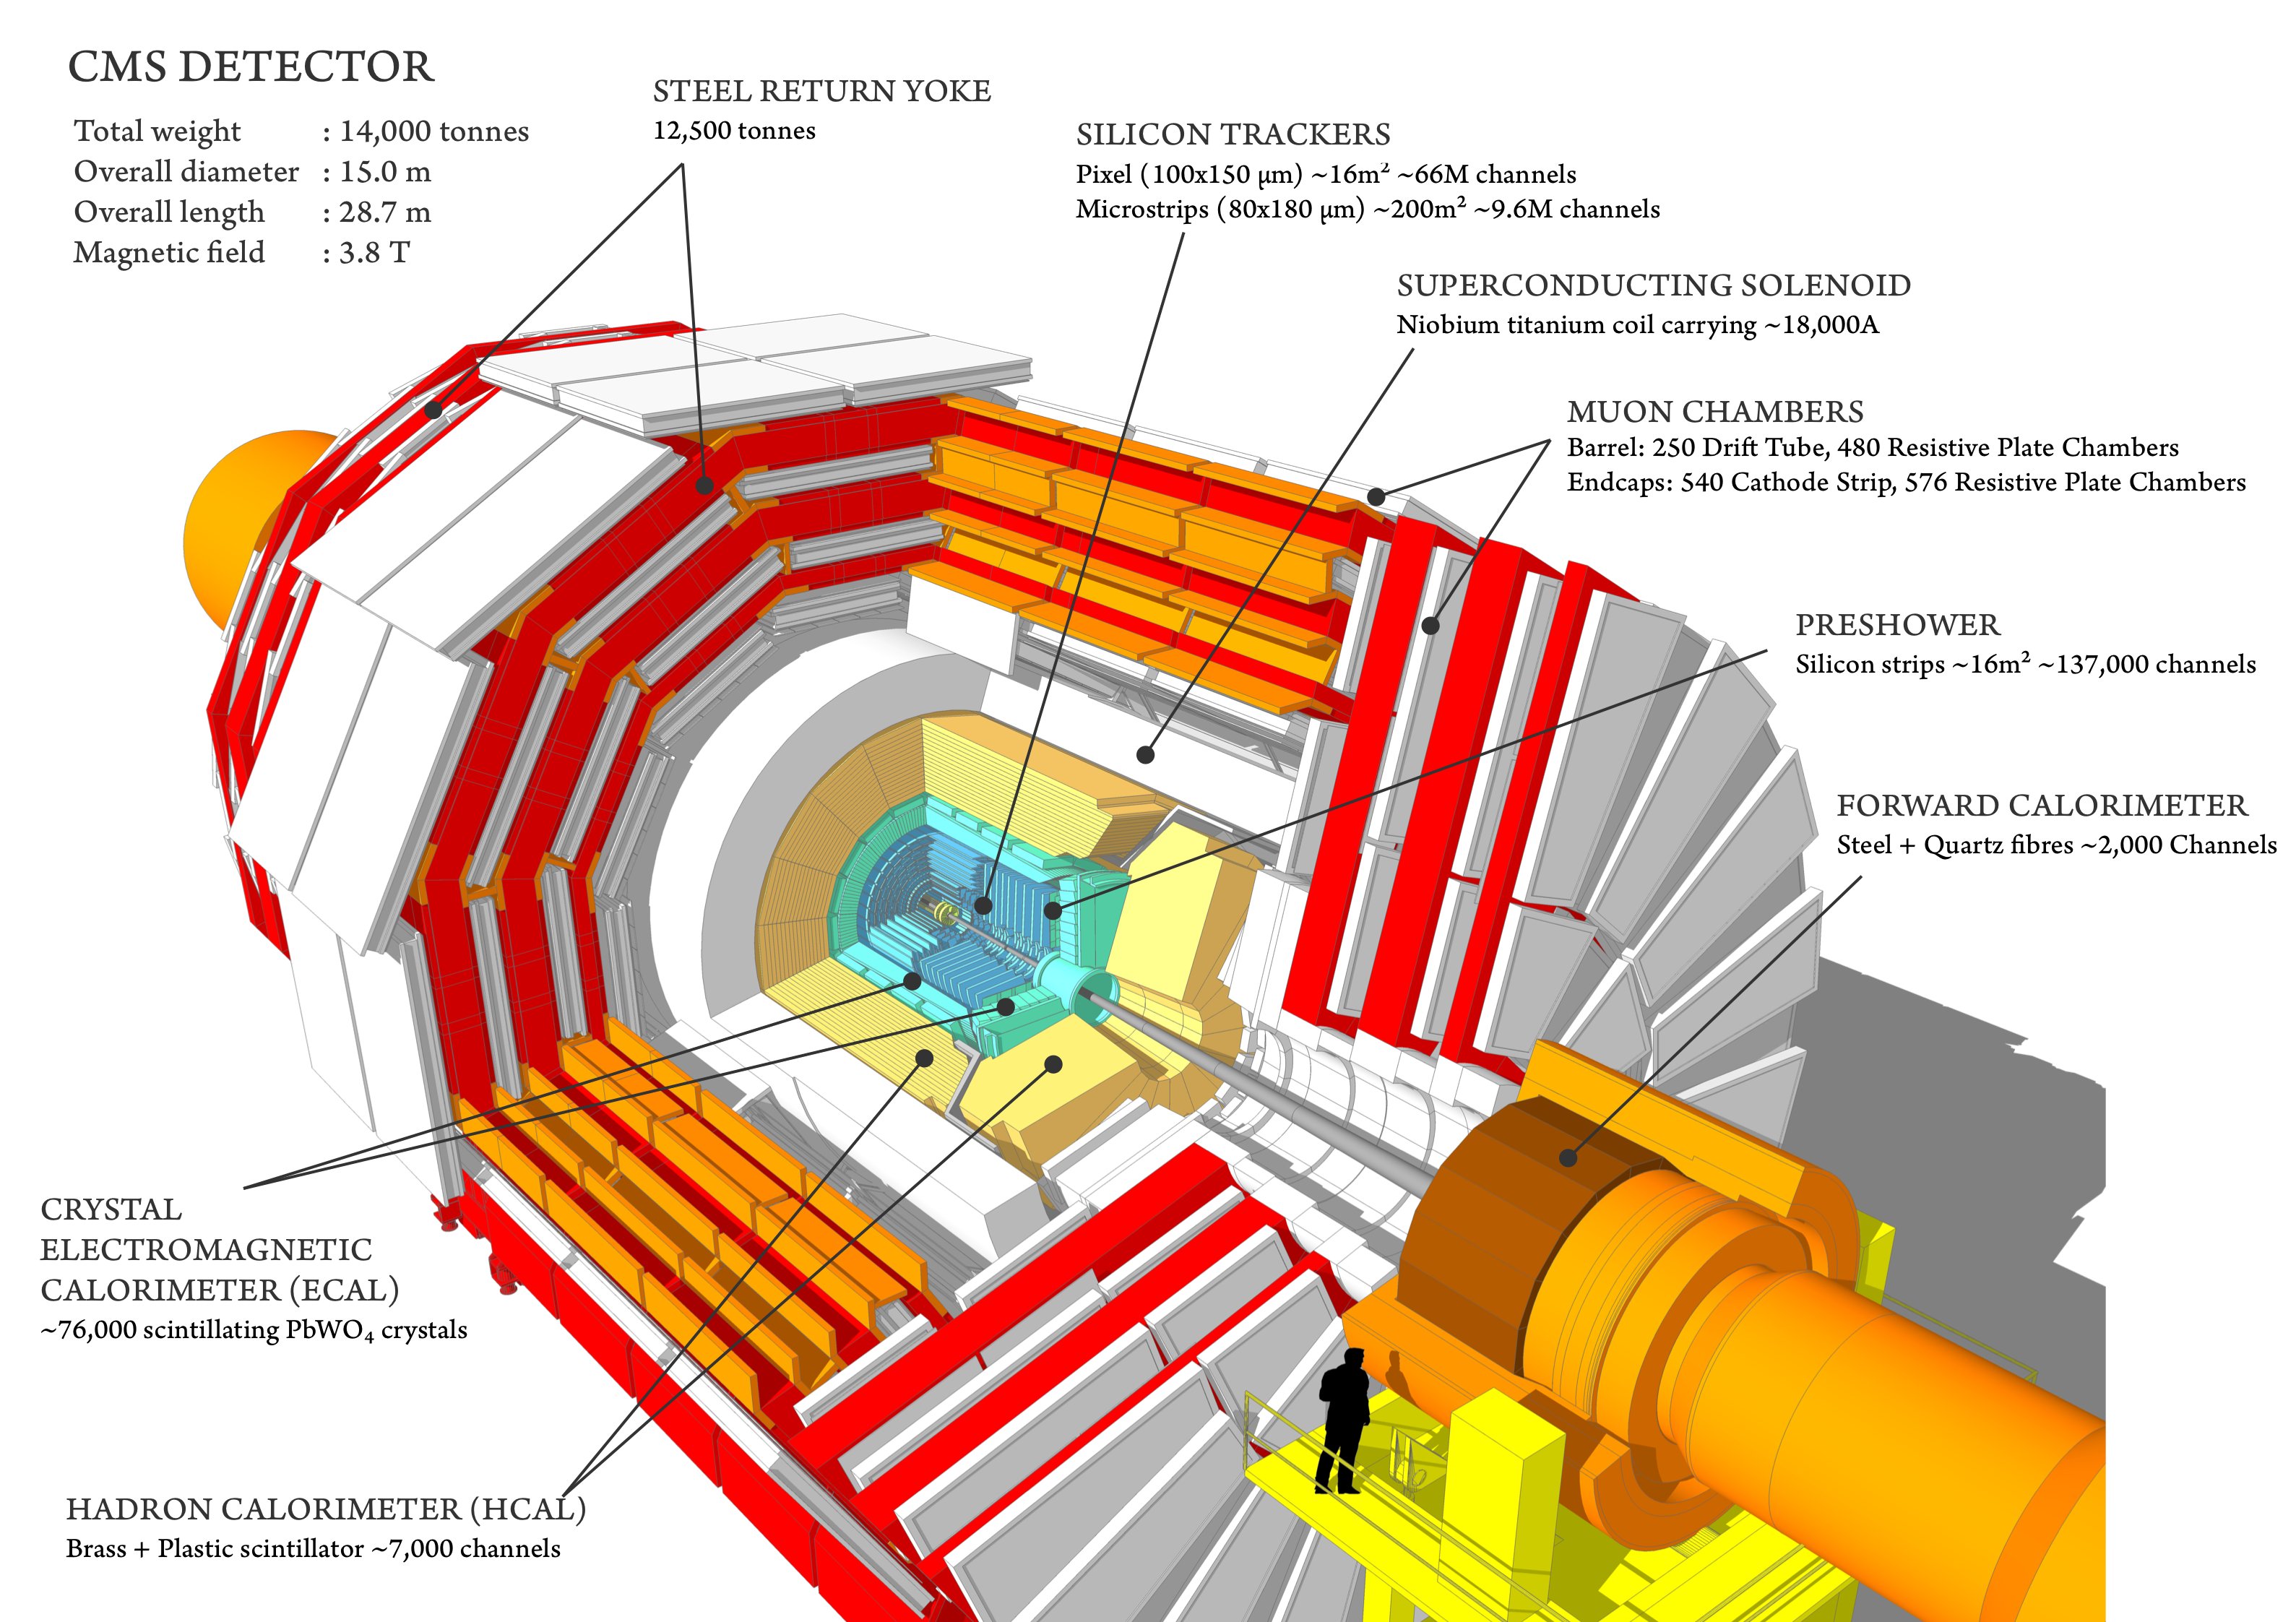
\includegraphics[width=0.99\textwidth]{figures/cms_sketch}\hfil
\caption{Sketch of the CMS experiment at the LHC, showing its different subdetectors stacked concentrically, like a cylindrical onion. }
\label{fig:cms_sketch}
\end{figure*}

Muons are long-lived particles that interact only via the electromagnetic and weak interactions. 
Differently from most of the particles produced at high energy collisions, they are able to go through all layers of CMS. 
Electrons, on the other hand, are stopped by the CMS Electromagnetic Calorimeter (ECAL), where they produce a particle shower based mostly on bremsstrahlung radiation (at high energies), and lose their energies almost completely. 
Due to the muons higher mass, they do not go through bremsstrahlung radiation as much as an electron, and therefore, is able to go through the CMS ECAL. 
Photons are measured by the ECAL in a similar way, the difference being that a photon shower starts by an electron-positron pair production from the original high energy photon. 
Muons also go through the CMS Hadronic Calorimeter (HCAL), which measures the energy of hadronic particles in a similar way that the ECAL measures the energy of photons and electrons, but with showers caused by the strong interaction. 

The CMS calorimeters are usually called destructive detectors, since, in order to measure the particle's energy, the particle must not leave the detector.
On the other hand, the tracking system aims to measure the particles' energy with little interaction to minimize the energy loss (so that it can be precisely measured by the calorimeters). 
This is performed, for example, through ionizing radiation on semi-conductor or gaseous devices. 

\subsection{The CMS Tracking Detectors}

The CMS tracking system must provide precise reconstruction for charged particles' trajectories with minimal interference in the particles' energies. 
These trajectories are reconstructed in terms of tracks, which are built from the different interactions of the incoming particle with the tracking system (hits). 
It must also cope with the high charged particle flux at various radii at high luminosity, which requires a high detector segmentation to reconstruct large track multiplicities at the same time. 

The CMS tracking system is entirely constructed of silicon, which detects hits by measuring electron-hole currents in the device produced by ionizing radiation. 
The geometry of these silicon sensors is different for three regions within the CMS detector, which are defined based on the charged particle flux from the LHC:

\begin{itemize}
\item  Closest to the interaction vertex where the particle flux is the highest, pixel detectors are placed. The size of a pixel is $\approx 100~\times~150 ~\mu$m$^{2}$, giving an occupancy of about 10$^{-4}$ hits per pixel per LHC crossing.
\item In the intermediate region ($20 < r < 55$ cm), the particle flux is low enough to enable use of silicon microstrip detectors with a minimum cell size of $10$ cm $\times~80~\mu$m, leading to an occupancy of $\approx 2-3\%$ per LHC crossing.
\item In the outermost region ($r > 55$ cm) of the inner tracker, the particle flux has dropped sufficiently to allow use of larger-pitch silicon microstrips with a maximum cell size of $25$ cm $\times~180~\mu$m, while keeping the occupancy to $\approx 1\%$.
\end{itemize}

The pixel layers of the CMS tracker consist of three cylindrical layers of pixel modules surrounding the interaction point at radii of 4.4,7.3 and 10.2 cm, and are topped at each side with two pixel module disks at $|z|$ = 34.5 cm and 46.5 cm. 
In total, it covers about 1 m$^{2}$, with 66 million pixels, and
The pixel detector delivers three high precision hits for each charged particle trajectory: the spatial resolution is measured to be about 10 $\mu$m for the $r-\phi$ measurement and about 20 $\mu$m for the $z$ measurement

After the pixels, the strip tracker detector covers the radial range between 20 cm and 116 cm. 
It consists of three different subsystems: the tracker inner barrel, inner disks and outer barrel (TIB, TID and TOB). 
The inner subsystems (TIB and TID) extend in radius from 20 cm to 55 cm, are composed of 4 layers in the barrel and 3 layers at each end, and deliver up to 4 measurements in $r-\phi$ by track, with a single hit resolution between 23 $\mu$m and 35 $\mu$m. 
The outer system (TOB) extends to a radius of 1.2m and to $|z| = 118$ cm, consists of 6 layers of micro-strip sensors, providing another 6 $r-\phi$ measurements with single point resolution between 35 $\mu$m and 53 $\mu$m. 

\begin{figure*}[h]
\centering 
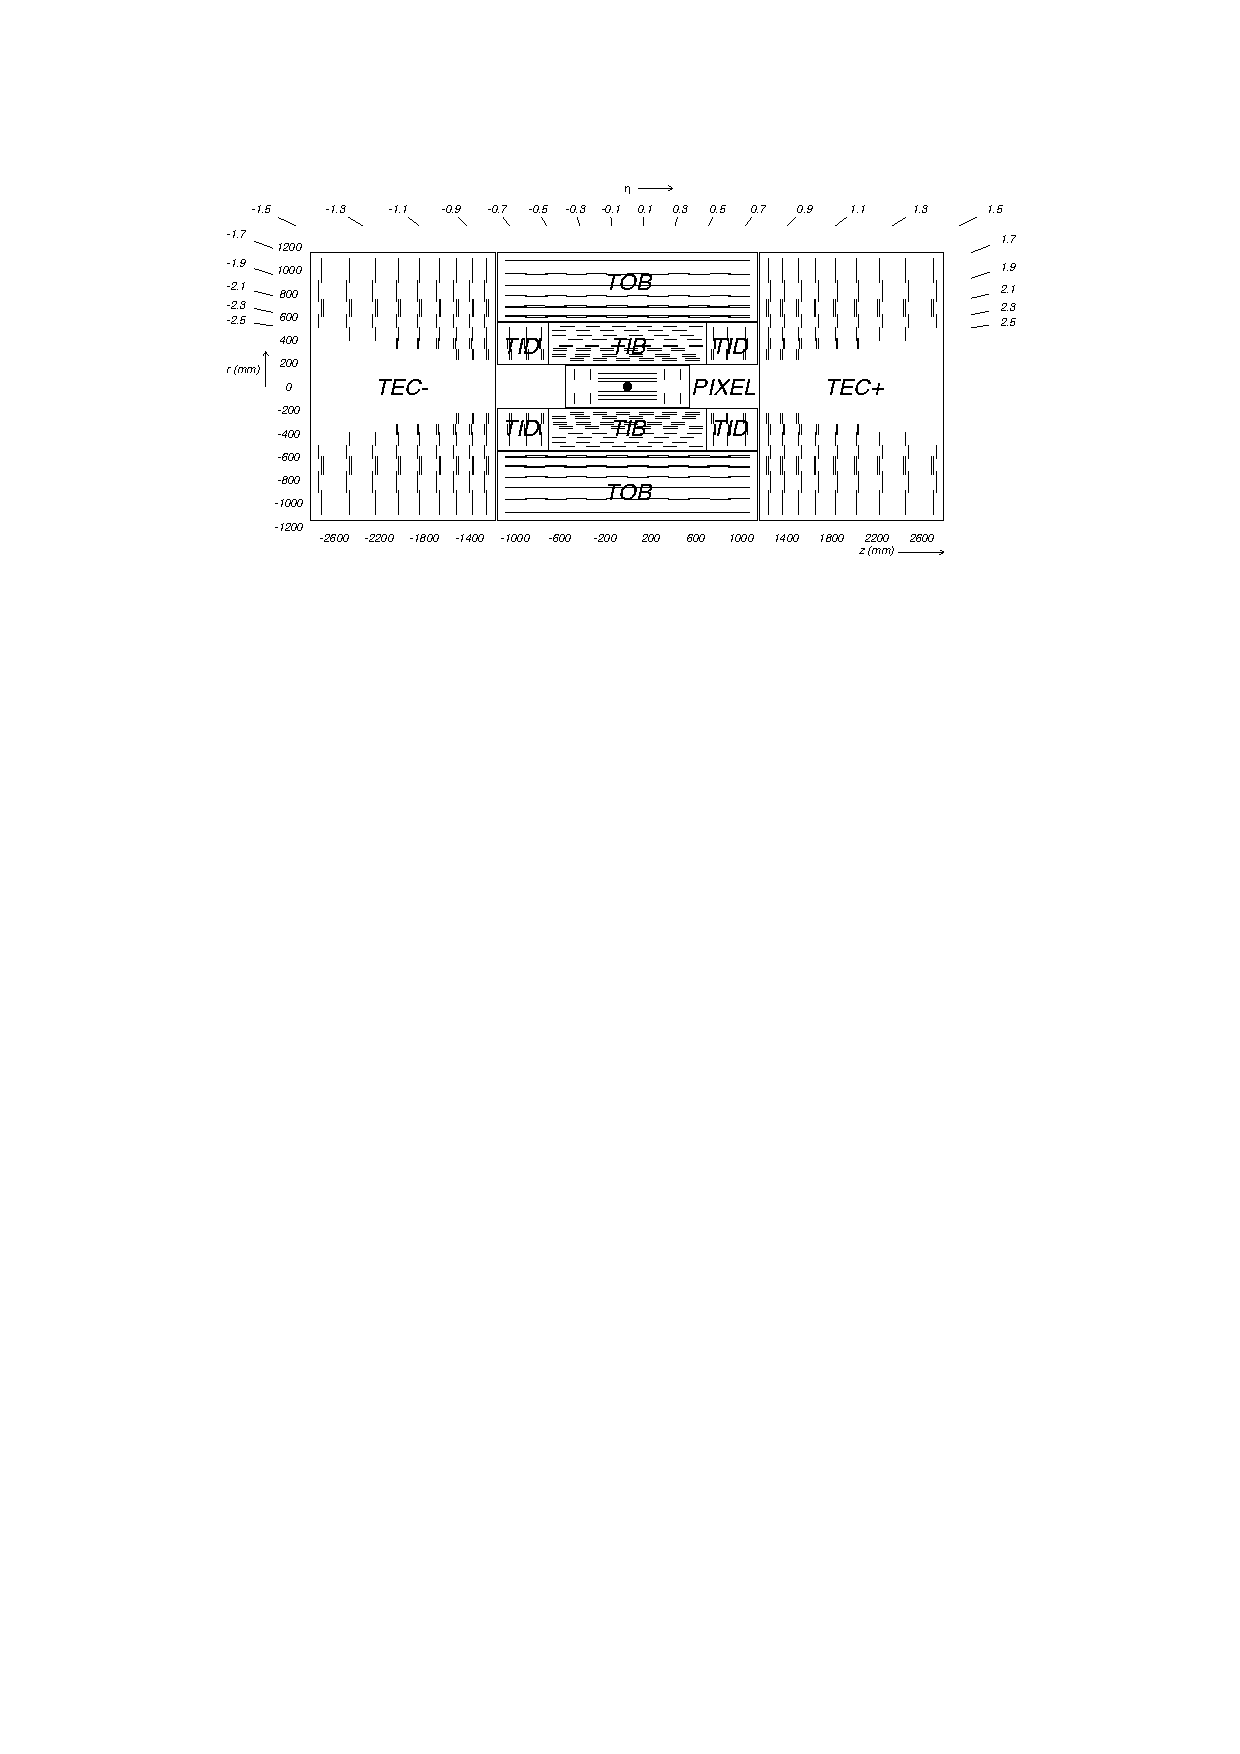
\includegraphics[width=0.99\textwidth]{figures/cms_tracker}\hfil
\caption{Sketch of the CMS tracker system. }
\label{fig:cms_tracker}
\end{figure*}


Beyond the TOB, the tracker endcaps (TEC+ and TEC-, where the sign relates to the location along the z axis) cover the region 124 cm $< |z| < $282 cm and 22.5 cm $< |r| <$ 113.5 cm. 
Each endcap consists of 9 disks, each with up to 7 rings of silicon micro-strips, providing up to 9 $r-\phi$ measurements per track. 
Additionally, some of the modules on the TIB, TID, TOB and TEC also carry a second micro-strip sensor module, mounted with a stereo angle of 100 mrad, to prove a measurement of the second coordinate (z in the barrel and r on the disks/endcaps). 
The overall CMS tracker module structure can be seen in Figure \ref{fig:cms_tracker}.


\subsection{The CMS Calorimetry Detectors}

The CMS calorimetry system consists of an electromagnetic calorimeter (ECAL), that measures the energies of electrons and photons, and a hadronic calorimeter (HCAL), that measures the energies of hadrons. 
The CMS HCAL will be described below, while the ECAL will be described in detail in Section \ref{sec_ecal}.

\subsubsection{The Hadronic Calorimeter}

The strong interaction forces quarks and gluons to hadronize, a process in which hadrons (particles consisting of quarks) to be produced copiously from an initial colored particles. Some of these hadrons are unstable and can further decay into stable particles (such as leptons and other stable hadrons). 
At the end of the hadronization process, a quark/gluon is seen by CMS as a cluster of mostly electrons (with photons from bremsstrahlung), muons, pions, kaons, protons and neutrons, which are combined to form an object called a jet. 
Therefore, for precise jet measurements, the CMS experiments must precisely measure the energy of hadrons within a jet shower. 

The HCAL is limited by the ECAL in its inner radius, and by the CMS solenoid in its outer radius. 
In order to provide hermeticity and full coverage of the hadronic shower development, it must maximize the amount of absorber material in its region. 
This absorber material is a dense material with a high atomic number that causes the hadrons within a jet to further decay into less energetic particles.
The energy of these further decays are then measured by an active medium. 

The CMS HCAL is divided into three sections, the barrel (HB), the outer barrel region just outside the CMS solenoid (HO), the endcaps (HE) and the forward region closer to the beam pipe (HF), which can be seen in Figure \ref{fig:cms_hcal}. 
The HB and HE consist of brass absorbers, as it has a reasonably short interaction length, is easy to machine and is non-magnetic, while the active medium consists of plastic scintillator tiles read out with embedded wavelength-shifting (WLS) fibres. 
The HO functions as a tail catcher and it consists of only a layer of active medium of plastic scintillator tiles. 
The forward calorimeter uses steel as absorber  and quartz fibers as active medium, a choice that is better suited for the more congested environment closer to the beam pipe. 
The photodetection readout is based on multi-channel hybrid photodiodes (HPDs) for HB, HE and HO, and on photomultiplier tubes (PMT) for HF.

\begin{figure*}[h]
\centering 
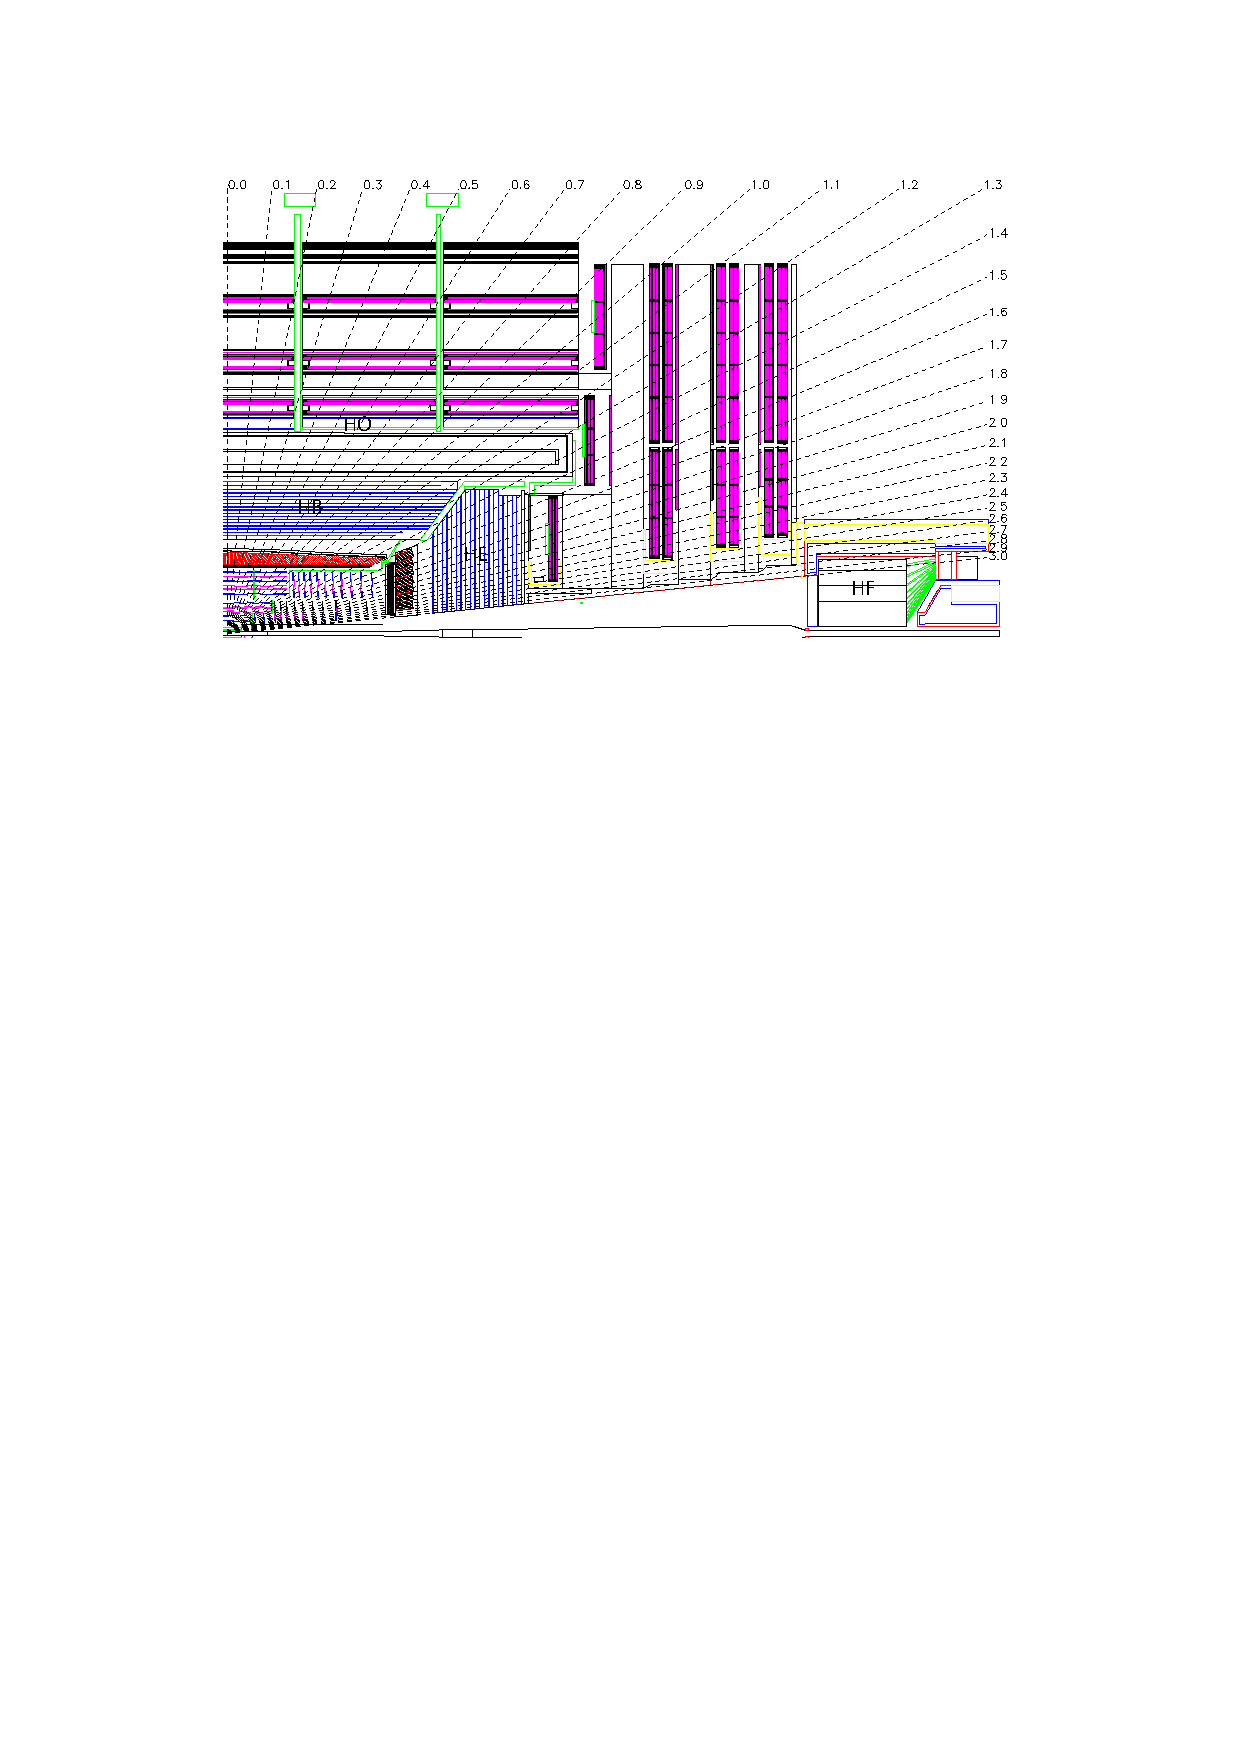
\includegraphics[width=0.99\textwidth]{figures/cms_hcal}\hfil
\caption{Sketch of the CMS hadronic calorimeter. }
\label{fig:cms_hcal}
\end{figure*}


The HB geometry consists of 32 towers covering the pseudorapidity region $-1.4 < \eta < 1.4$, resulting in 2304 towers with a segmentation $\Delta\eta\times\Delta\phi = 0.087\times0.087$.
Each HCAL endcap consists of 14 $\eta$ towers with $5^{o}$ $\phi$ segmentation, covering the pseudorapidity region $1.3 < |\eta| < 3.0$. 
For the 5 outermost towers (at smaller $\eta$) the $\phi$ segmentation is $5^{o}$ and the $\eta$ segmentation is 0.087. For the 8 innermost towers the $\phi$ segmentation is $10^{o}$, while the $\eta$ segmentation varies from 0.09 to 0.35 at the highest $\eta$. The total number of HE towers is 2304.
The HO detector contains scintillators with a thickness of 10 mm, which line the outside of the outer vacuum tank of the solenoid and cover the region $-1.26 < \eta < 1.26$. The tiles are grouped in $30^{o}$-sectors, matching the $\phi$ segmentation of the muon chambers to which it is attached. 
Coverage between pseudorapidities of $3.0 < |\eta| < 5.0$ is provided by the HF calorimeter. 
There are 13 HF towers in $\eta$, all with a size given by $\Delta\eta\approx0.175$, except for the lowest-$\eta$ tower with $\Delta\eta\approx0.1$ and the highest-$\eta$ tower with $\Delta\eta\approx0.3$. 
The $\phi$ segmentation of all towers is 10$^{o}$, except for the highest-$\eta$ one which has $\Delta\phi= 20^{o}$. 
This leads to 900 towers and 1800 channels in the 2 HF modules.

\subsection{The CMS Muon Detectors}

Because of its mass, muons bend less under a magnetic field than electrons of the same momentum. 
Therefore, in order to precisely determine the momentum of muons, an extra tracking system must be added to CMS outside the solenoid. 
The CMS muon system is divided into two sections, with two different detector technologies in each: the drift tubes (DT) and resistive place chambers (RPC) located in the barrel, and the cathode strip chambers (CSC) and RPCs in the endcaps. 
These three technologies are based on gaseous detectors, differing on the geometry of the cell in which the gas is trapped and on the collection of charge from the gas ionization process due to the incoming muon. 
While the DTs and the CSCs are particularly suited for a precise determination of the muon's momentum, the RPCs provide a fast signal with good time resolution, but coarser spatial precision. 
The RPCs are used for bunch crossing determination in the muon system. 
Figure \ref{fig:cms_muon} shows a sketch of the muon system, highlighting its three different components. 

\begin{figure*}[h]
\centering 
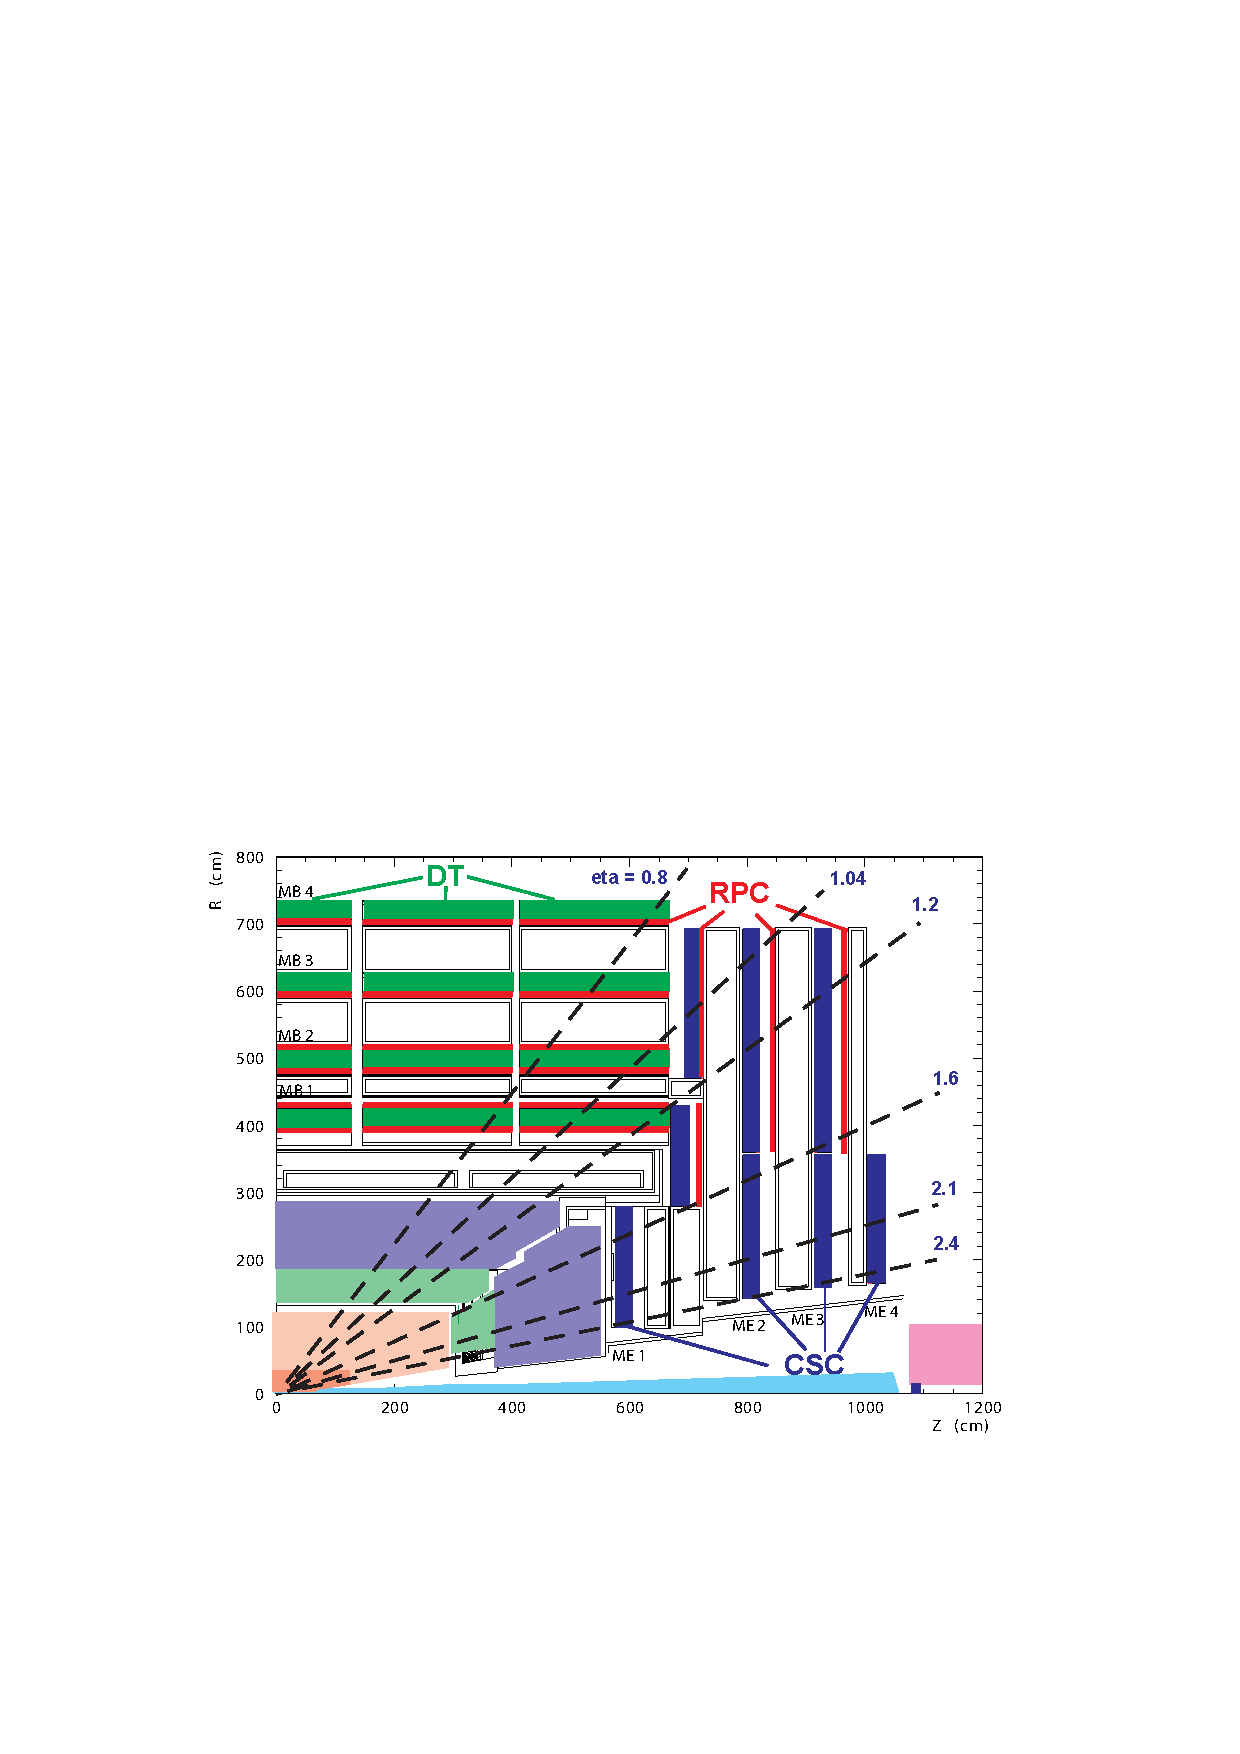
\includegraphics[width=0.9\textwidth]{figures/cms_muon}\hfil
\caption{Sketch of the CMS muon detectors. }
\label{fig:cms_muon}
\end{figure*}


In the barrel, the muon system is organized in chambers divided into 4 layers at radii of approximately 4.0, 4.9, 5.9 and 7.0 m from the beam axis. 
The layers are organized in 5 wheels along the beam axis, covering in total the region $|\eta| < 1.2$, and each wheel is divided into 12 stations, with each covering a $30^{o}$ azimuthal angle. 
Chambers in different stations are organized so that a high-p$_T$ muon produced near a sector boundary crosses at least 3 out of the 4 stations in each layer. 
Each station is designed to give a muon vector in space, with a $\phi$ precision better than 100 $\mu$m in position and approximately 1 mrad in direction. 
In the two innermost layers, each DT chamber is coupled between two RPCs, while, in the two outermost layers, each chamber is coupled to one RPC.

In each of the endcaps, the CSCs and RPCs are arranged in 4 disks perpendicular to the beam, and in concentric rings, 3 rings in the innermost station, and 2 in the others, totaling in 486 CSC chambers for both endcaps. 
The chambers are trapezoidal and cover either 10$^{o}$ or 20$^{o}$ in $\phi$. 
A muon in the pseudorapidity range $1.2 < |\eta | < 2.4$ crosses 3 or 4 CSCs. 
In the endcap-barrel overlap range, $0.9 < |\eta | < 1.2$, muons are detected by both the barrel DTs and endcap CSCs. 
The spatial resolution provided by each chamber from the CSCs is typically about 200 $\mu$m (100 $\mu$m for the innermost layer). The angular resolution in $\phi$ is of the order of 10 mrad.

\subsection{Luminosity Detectors}

The instantaneous luminosity is a key element to perform physics analysis at colliders in order to estimate how many events a certain process will yield given its cross section. 
The CMS experiment uses five different detectors to monitor and measure the instantaneous luminosity, based on different occupancy measurements for each individual detector. 
The used subdetectors are: the barrel DTs, the HF, the Pixel Luminosity Telescope (PLT) and the Fast Beam Condtions Monitor (BCM1f). 
The last two detectors use silicon pixel sensors and single-crystal diamonds, respectively, located close to the LHC beam pipe. 

These luminosity measurements are calibrated with dedicated LHC runs called Van der Meer (VdM) scans. 
By scanning the two beams through one another in the transverse plane of the detector, VdM scans allow to measure the luminosity per colliding bunch pair from machine parameters. 

\subsection{The CMS Trigger and Data Acquisition Systems}

The LHC provides bunch crossings with intervals of 25ns, which means that CMS produces collisions data at a rate of 40 MHz. 
The average event size produced by the CMS data acquisition system is of about 1 MB, which means that, if the experiment were to read and save every collision, it would need a data output bandwidth of approximately 40 TB/s. 
Such amount of data cannot be processed and saved by the current capabilities of the computing farms responsible for these tasks. 
However, most of these events are not of interest for the experiment: they consist of low energy QCD processes which would not be selected, in general, by any physics analysis. 
For this reason, CMS uses a trigger system that filters the collision data online. 
In general terms, the CMS trigger system must ensure a large acceptance for physics signals, while keeping the output rate and CPU time under control.

The first layer of the CMS trigger system is called the Level-1 (L1) trigger, and reduces the event rate from 40 MHz to 100 kHz. 
It works at hardware level, based on FPGA and custom ASIC integrated circuits technology, using information from the calorimeters and muon detectors to select, in about 4 $\mu$s, the most interesting events. 

The L1 is divided into three parts: the calorimeter trigger, the muon trigger and the global trigger.
The calorimeter trigger is itself divided into two steps: Layer-1 and Layer-2. 
In the first, it receives summarized data from the ECAL and HCAL in small packets called trigger primitives and computes basic information such as the sum of ECAL and HCAL energies and energy calibration as well as the computation of the H/E ratio (used to discriminate electrons and photon from hadronic jets). 
The information calculated by the Layer-1 is parallelized: each Layer-1 processor calculated local information pertaining to a section of the detector. 
The following step, the Layer-2 calorimeter trigger, receives the information from the Layer-1 and calculates global variables (such as total energy sum and calorimeter based missing transverse energy) and reconstructs simple versions of jets, taus and electrons/photons. 

The muon trigger receives information from the three muon subdetectors to ensure good coverage and redundancy. 
For the DTs and CSCs, the front-end trigger electronics identifies track segments from the hit information registered in multiple detector planes of a single measurement station, which are transmitted via optical fibers to regional track finder processors. 
These processors apply pattern recognition algorithms to identify muon candidates and measure their momenta from their bending under the CMS magnet. 
The combined muon trigger provides to the global trigger the transverse momentum of the muon candidates, along with their positions and quality scores, so they can be accepted/discarded by the global trigger. 

The global trigger, the final L1 step, is responsible for selecting interesting events based on the global information received from the Layer-2 calorimeter trigger and the last step of the muon trigger. 
These decisions are taken based on L1 selection algorithms stored in the electronics. 
This decision is informed to the central CMS data acquisition system, which transmits the full event data to processors that will format the data for the next trigger step, the High Level Trigger (HLT). 

The HLT is the final online selection step at CMS, and reduces the event rate from 100 kHz (L1 output) to a sustainable level of 1 kHz. 
It is implemented in software running on a farm of commercial computers which includes about 16,000 CPU cores. 
The HLT runs a simplified version of the full CMS object reconstruction, detailed below, based on the CMS software architecture CMSSW, optimized for the CPU timing requirements that exist at trigger level. 


\subsection{Object Reconstruction at CMS}

The general object reconstruction at CMS can be summarized in Figure \ref{fig:cms_reco}. 
It takes advantage of the CMS geometry, the cylindrical onion, and gathers information from different subdetectors to reconstruct a single type of particle: charged hadrons will leave hits in the tracker and will be stopped by the HCAL; neutral hadrons will not leave hits in the tracker but will deposit their energy on the HCAL; electrons and photons will both deposit their energies on the ECAL, while the former will also leave hits in the tracker; muons will leave hits in the tracker and the muon system, with no energy deposits in the calorimeters. 
This global event description, which links information from the different subdetectors, is usually referenced as particle flow algorithms (PF). 
The particles created with this event description are called PF candidates and are mutually exclusive. 
This means, for example, that a single track cannot be used to reconstruct two different PF candidates.
It's important to notice that using particle flow algorithms at CMS is only possible due to the high granularity and position resolution of all its parts, particularly its calorimeters. 

\begin{figure*}[h]
\centering 
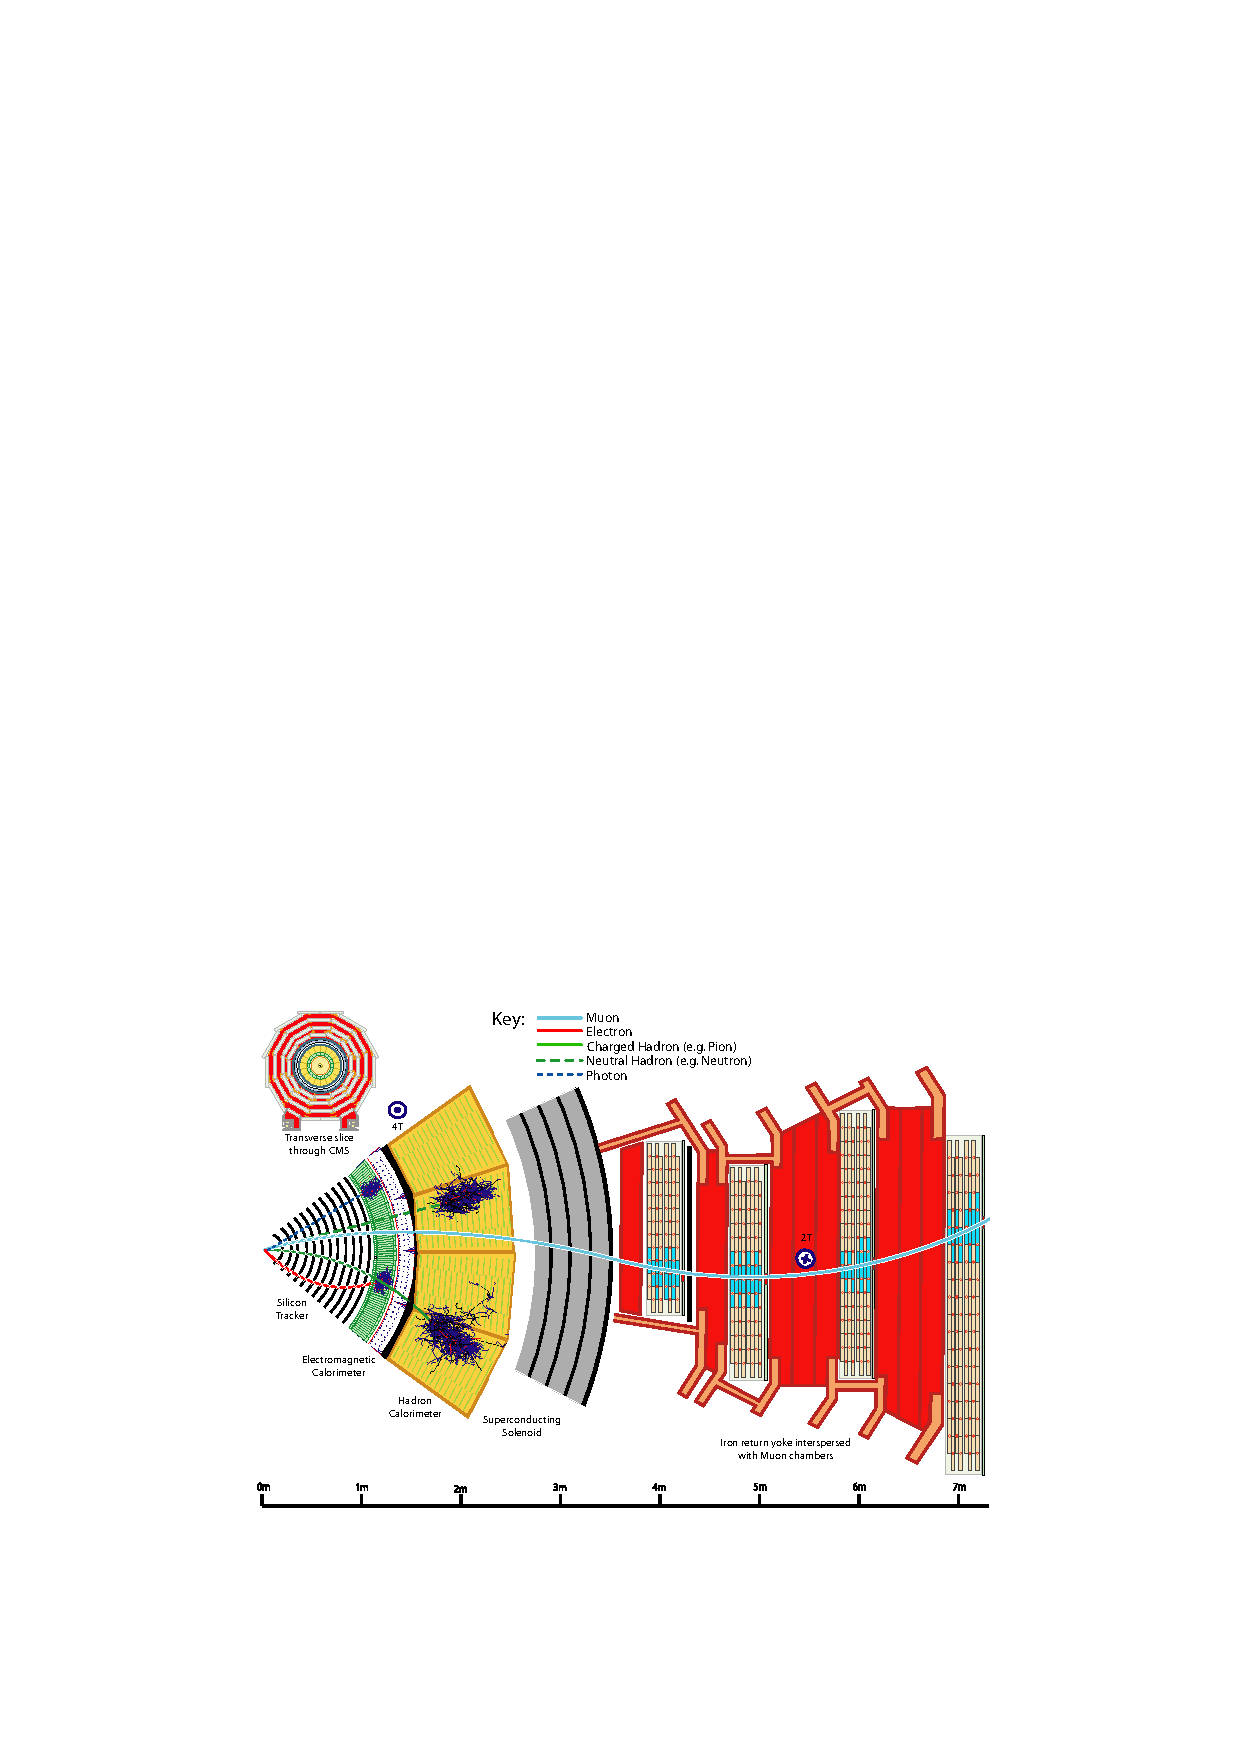
\includegraphics[width=0.9\textwidth]{figures/cms_reco}\hfil
\caption{Sketch of different types of object reconstruction at CMS. }
\label{fig:cms_reco}
\end{figure*}

The basic ingredients of the particle flow algorithm are the energy clusters on the calorimeters and the reconstructed trajectories obtained from the trackers and muon systems, which will be discussed below.  
Then, some of the objects reconstructed by CMS will be described, particularly the ones that are important in the analyses to be described in the following section.

\subsubsection{Particle Flow Ingredients}

Tracks are the reconstructed trajectories of charged particles that leave hits in the CMS tracker. 
Other than providing position information, these tracks are used to measure the particle's momentum via its bending under the CMS magnet. 
Track reconstruction starts with clusters of hits close to the beam pipe, in the inner pixel detector. 
Possible trajectories are then extrapolated and, if hits in the following tracker layers are found, they are added to the track and the track parameters are updated. 
After the algorithm hits the final tracker layers, and a first version of the full trajectory is reconstructed, another track reconstruction is performed, this time outside-in. 
The final track parameters are set to the weighted average of inside-out and outside-in results. 
The tracks have to fulfill quality criteria and are otherwise discarded. 
Finally, the used tracker hits are removed from the hit collection, and the procedure is repeated.

Primary vertices, which represent the point where a hard scatter event occurred during a bunch crossing, are reconstructed based on track clustering at the interaction region. 
This region is at the center of CMS and has a typical length of $\approx$ 5-6 cm in the z direction, while its transverse dimension is $\approx$ 20-30 $\mu$m. 
Many primary vertices can be reconstructed for one bunch crossing. 
During the 2016 data taking period, events with over 50 primary vertices have been recorded by CMS. 
It is common to refer to the number of reconstructed primary vertices as "pile-up".

The fitting procedure used to extrapolate the tracks in the usual reconstruction does not perform well for electron tracks. 
This happens because of the high amount of bremsstrahlung radiation electrons emit in the tracker, changing considerably the expected shape of their trajectory, which is not modeled by the standard algorithm. 
The electron-like tracks, selected based on their original fit quality and number of hits, are then refitted with a more appropriate method, the Gaussian-sum Filter (GSF), which allows for substantial non-Guassian energy loss along the trajectory.

Calorimeter clusters are reconstructed to detect and measure the energy of photons, electrons and hadrons, being the only source of measurement for photons and neutral hadrons. 
The clustering algorithm, that gathers in groups calorimeter deposits, is applied separately for the different calorimeter partitions: ECAL barrel, ECAL endcaps, HCAL barrel, HCAL endcaps, and each of the two preshower layers. 

The clustering procedure starts by searching for cluster seeds, which are local calorimeter-cell energy maxima, with respect to either its closest 8 or 4 cells, above a certain threshold. 
Topological clusters are grown from cluster seeds by adding together nearby seeds that share calorimeter cells. 
These topological clusters are used to estimate the energy sharing between clusters reconstructed from two different but nearby cluster seeds. 
Each individual cluster position is calculated as $X=\sum_{i}(w_{i}X_{i})/(\sum_{i}w_{i})$, with $w_{i}=ln(E_{i}/E_{th})$, where $E_{th}$ is an energy threshold and the $i$ is summed over the cells within a cluster.

\subsubsection{Photons and Electrons}

Electrons are reconstructed based on seed electron tracks reconstructed with the GSF algorithm. 
After a good quality electron track is found, it must be linked to an energy cluster on the ECAL. 
Photons, on the other hand, rely solely on the ECAL clusters to be reconstructed, since they leave no signal on the trackers. 
The reconstruction algorithm for ECAL clusters, called supercluster algorithm, allows almost complete recovery of the energy of photons that convert due to the material in front of the ECAL. 
A detailed description of the algorithm can be found in Ref. [4]. 
The corrections and calibrations involved to ensure a precise energy reconstruction for these particles will be described in the section dedicated to the CMS ECAL. 

Photons are identified based on a set of shower shape and isolation variables. 
The former measures the shape of the energy deposit on the ECAL, while the latter gives information about the event content surrounding the photon candidate. 
Isolation variables are particularly important when dealing with $\pi^{0}$ mesons, produced in hadronic showers, that decay to two almost colinear photons. 
These $\pi^{0}\rightarrow\gamma\gamma$ objects from jets must be filtered out of the photons collection in a physics analysis looking for photons coming from the hard scatter interaction. 
Shower shape variables also help to distinguish between between real photons and jets, but also give important information against non-collision backgrounds reconstructed as photons. 

For the ECAL, electron and photon clusters look approximately the same, therefore, almost indistinguishable when using only calorimeter information. 
In order to separate electrons from the photon collection, one must veto on possible tracks appearing within the photon cone. 
This is done in two different ways in CMS: via a conversion-safe electron veto, which vetos on electron tracks that are not compatible with photon conversion tracks, and via the pixel seed veto, which vetos on hits in the innermost layers of the pixel detector assuming the photon cone coming from a certain primary vertex.

\subsubsection{Jets}

As mentioned above, colored particles cannot be observed in a color non-neutral state. 
Therefore, we can only access the information (such as kinematics) about a quark/gluon in the final state experimentally through its hadronization product, the jets. 
The process of obtaining a jet from a quark or a gluon, however, cannot be modeled by perturbative calculations, making it susceptible to many theoretical uncertainties and causing a "jet" to be ill-defined theoretically. 
There are, however, methods of jet reconstruction that minimize those uncertainties. 

The anti-$k_t$ and the Cambridge-Aachen (CA) methods are currently used by CMS and provide a jet reconstruction that are both infrared safe (avoiding low energy non-perturbative singularities) and colinear safe (avoiding singularities due to radiation colinear to the hadronizing particle). 
Both algorithms work by combining PF candidates sequentially in a jet if a certain distance discriminant is smaller than a certain parameter. 
The analyses documented in this document use the anti-$k_t$ algorithm with a distance parameter $R=0.4$, as most analyses using the CMS Run 2 dataset.

The energy of the reconstructed jets must be corrected in order to match a jets produced with particles generated from a full Monte Carlo simulation of a hadronization process. 
This mismatch is attributed to the nonuniform and nonlinear response of the CMS calorimeters, electronics noise and pile-up. 
To correct for this, jet energy correction (JEC) factors are derived centrally by the CMS collaboration to be used by individual analyses. 
These JEC factors correct the (raw) 4-momenta parameters of the reconstructed jet as a multiplicative factor.

An important contributor to performance degradation in jet energy measurement is the pile-up. 
Extra charged hadrons from the softer primary vertices can be erroneously clustered within the jet and bias the energy reconstruction. 
Therefore, a pile-up subtraction method that is called Charged Hadron Subtraction (CHS) is used in CMS. 
This is a particle-by-particle method that makes use of PF jets and exploits the excellent CMS tracking capabilities to identify and remove charged hadrons inside jets that are known to originate from pile-up vertices.

\subsubsection{Identification of b-quark jets}

Many interesting phenomena that is searched at the LHC involves bottom quarks. 
One important example is the $H\rightarrow b\bar{b}$ process, which has the highest branching fraction among the SM Higgs decays. 
Another example is the top quark decay, which is almost always to a bottom quark plus a W boson. 
These searches would be facing an enormous amount of background events if jets from bottom quarks were indistinguishable from lighter quark jets, copiously produced by the LHC. 
However, bottom quark jets (from now on simply referred to as b-jets) are strikingly different from their lighter counterparts due to the presence of a B meson (product of the bottom quark hadronization). 

B mesons can only decay via the weak interaction via a Cabbibo suppressed processes $b\rightarrow Wc$ and $b\rightarrow Wu$. 
This causes the average lifetime of a B meson to be of about 1.5 picoseconds. 
Assuming they are produced at the speed of light, these mesons can travel around 0.5 milimeters before decaying. 
This decay length is well within the reach of the current CMS tracking resolution, therefore, the vertex of the B meson decay can be measured. 
With this information, algorithms (b-taggers) can be constructed to distinguish b-jets from light jets.

The b-tagger algorithm utilized in the analyses presented in this thesis is the Combined Secondary Vertex (CSV) algorithm. 
This method uses multiple reconstruction quantities related to the tracks associated to the jet constituents and the properties of secondary vertices reconstructed inside the jet, if present. 
The CSV algorithm is still applicable, however, when no secondary vertices are associated to the jet. 
The variables used by this method include the number of tracks in the jet, the significance of the tracks? impact parameters, and, if available, the impact parameter, mass and number of tracks associated to the secondary vertex. 
These variables are used to determine a single likelihood discriminator associated to the jet, i.e. the CSV discriminator, proportional to the compatibility of the jet with a b-quark decay.














\chapter{The CMS Electromagnetic Calorimeter}
\label{sec_ecal}
\graphicspath{{ecal/figures/}{ecal/}}


The CMS ECAL is a high-resolution, hermetic, and homogeneous electromagnetic calorimeter made of 75,848 scintillating lead tungstate crystals divided among a barrel ($|\eta| < 1.48$) and two endcaps ($1.48 < |\eta| < 3.0$) \cite{ECALTDR}, as shown in Figure \ref{fig:ecal_sheme}. 
%These crystals are characterized by fast light emission, short radiation length ($X_0 = 0.89$ cm) and small Moliere radius ($R_M = 2.10$ cm). 
The light emitted by these crystals is detected with avalanche photodiodes (APDs) in the barrel and vaccuum photontriodes (VPTs) in the endcaps. The signal readout is performed with two avalanche photodiodes (APDs) per crystal in the barrel, and one vacuum phototriode (VPT) in the endcaps. These characteristics, translated into precise energy and timing resolutions, are an invaluable tool for the CMS physics program.

\begin{figure*}[bh]
\centering 
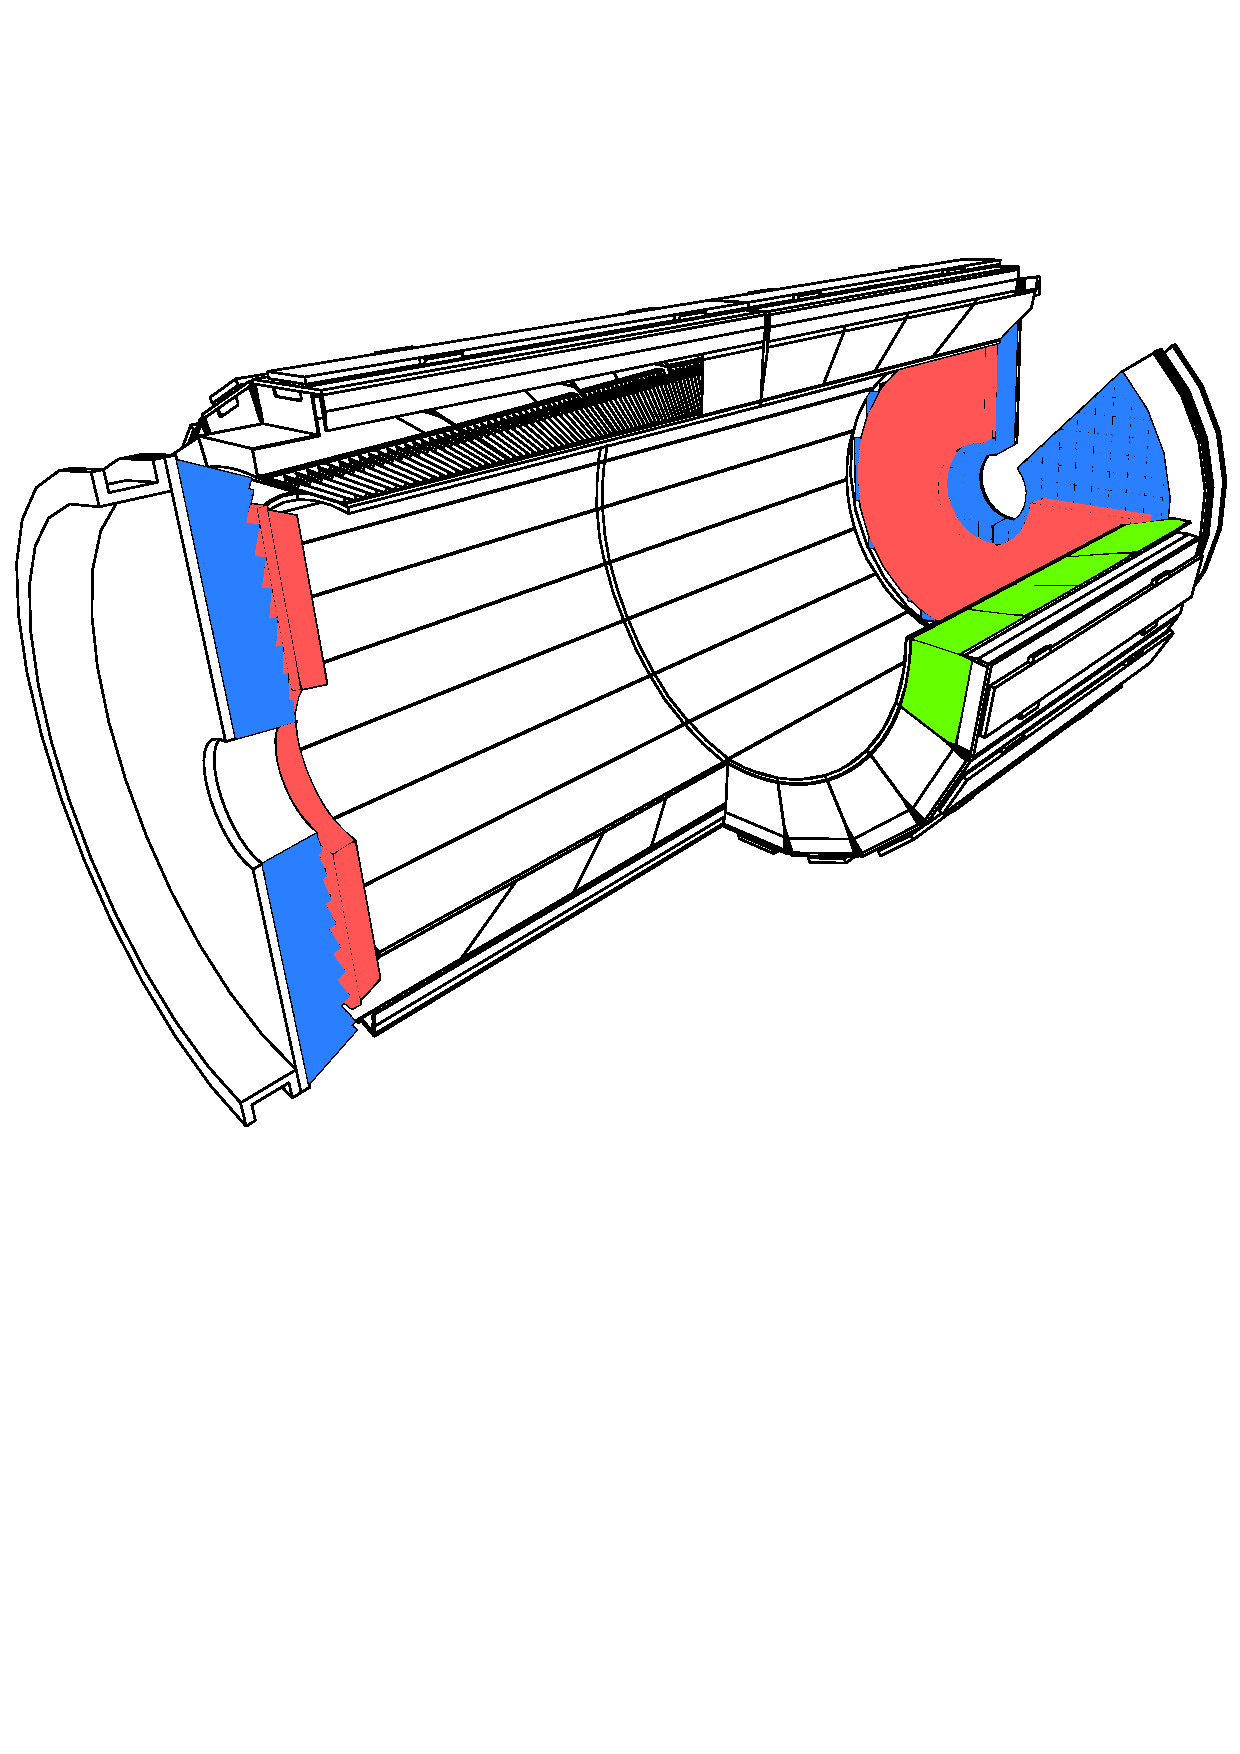
\includegraphics[width=0.7\textwidth]{figures/ECAL_scheme}\hfil
\caption{The CMS ECAL scheme highlighting a barrel supermodule (green), the ECAL endcaps (blue) and the ECAL preshower (red). }
\label{fig:ecal_scheme}
\end{figure*}


Completing the CMS electromagnetic calorimeter system is a preshower detector (ES), based on lead absorbers equipped with silicon strip sensors. It is installed in front of the ECAL endcaps, covering the region $1.65 < |\eta| < 2.6$. The fine granularity of the ES strips (2 mm wide) can resolve the signals of high-energy photons from the decays of neutral pions into two photons, when the separation angle between the photons is small, and can determine precisely the position of the electromagnetic deposits.

During the first year of Run II data taking at 13 TeV, the LHC provided a challenging environment, with one bunch crossing every 25 ns and an average of 10 interactions per crossing (pile up). This is expected to be even more challenging in 2016, with up to 40 pile up interactions. In the 2015 data taking period, the CMS ECAL operated with more than $98\%$ of its channels active, and was responsible for less than $7\%$ of CMS downtime during physics runs.


%\section{Detector Components}
\section{PbWO$_4$ Crystals and In-detector Electronics}

The main component of the ECAL are the lead tungstate crystals, that serve as both active material and absorber, constituting a homogeneous calorimeter. 
The barrel and endcap crystals are shaped as trapezoidal prisms, with 23 and 22 cm of length, respectively, consisting of about 26$X_{O}$. 
The crystal's front face (facing the interaction point) has an area of approximately $22\times22$ mm$^{2}$ (about $\Delta\eta\times\Delta\phi = 0.0175\times0.0175$) for the barrel and $25\times25$ mm$^{2}$ for the endcaps. 
Examples of such crystals are seen in Figure \ref{fig:ecal_crystals}.

\begin{figure*}[h]
\centering 
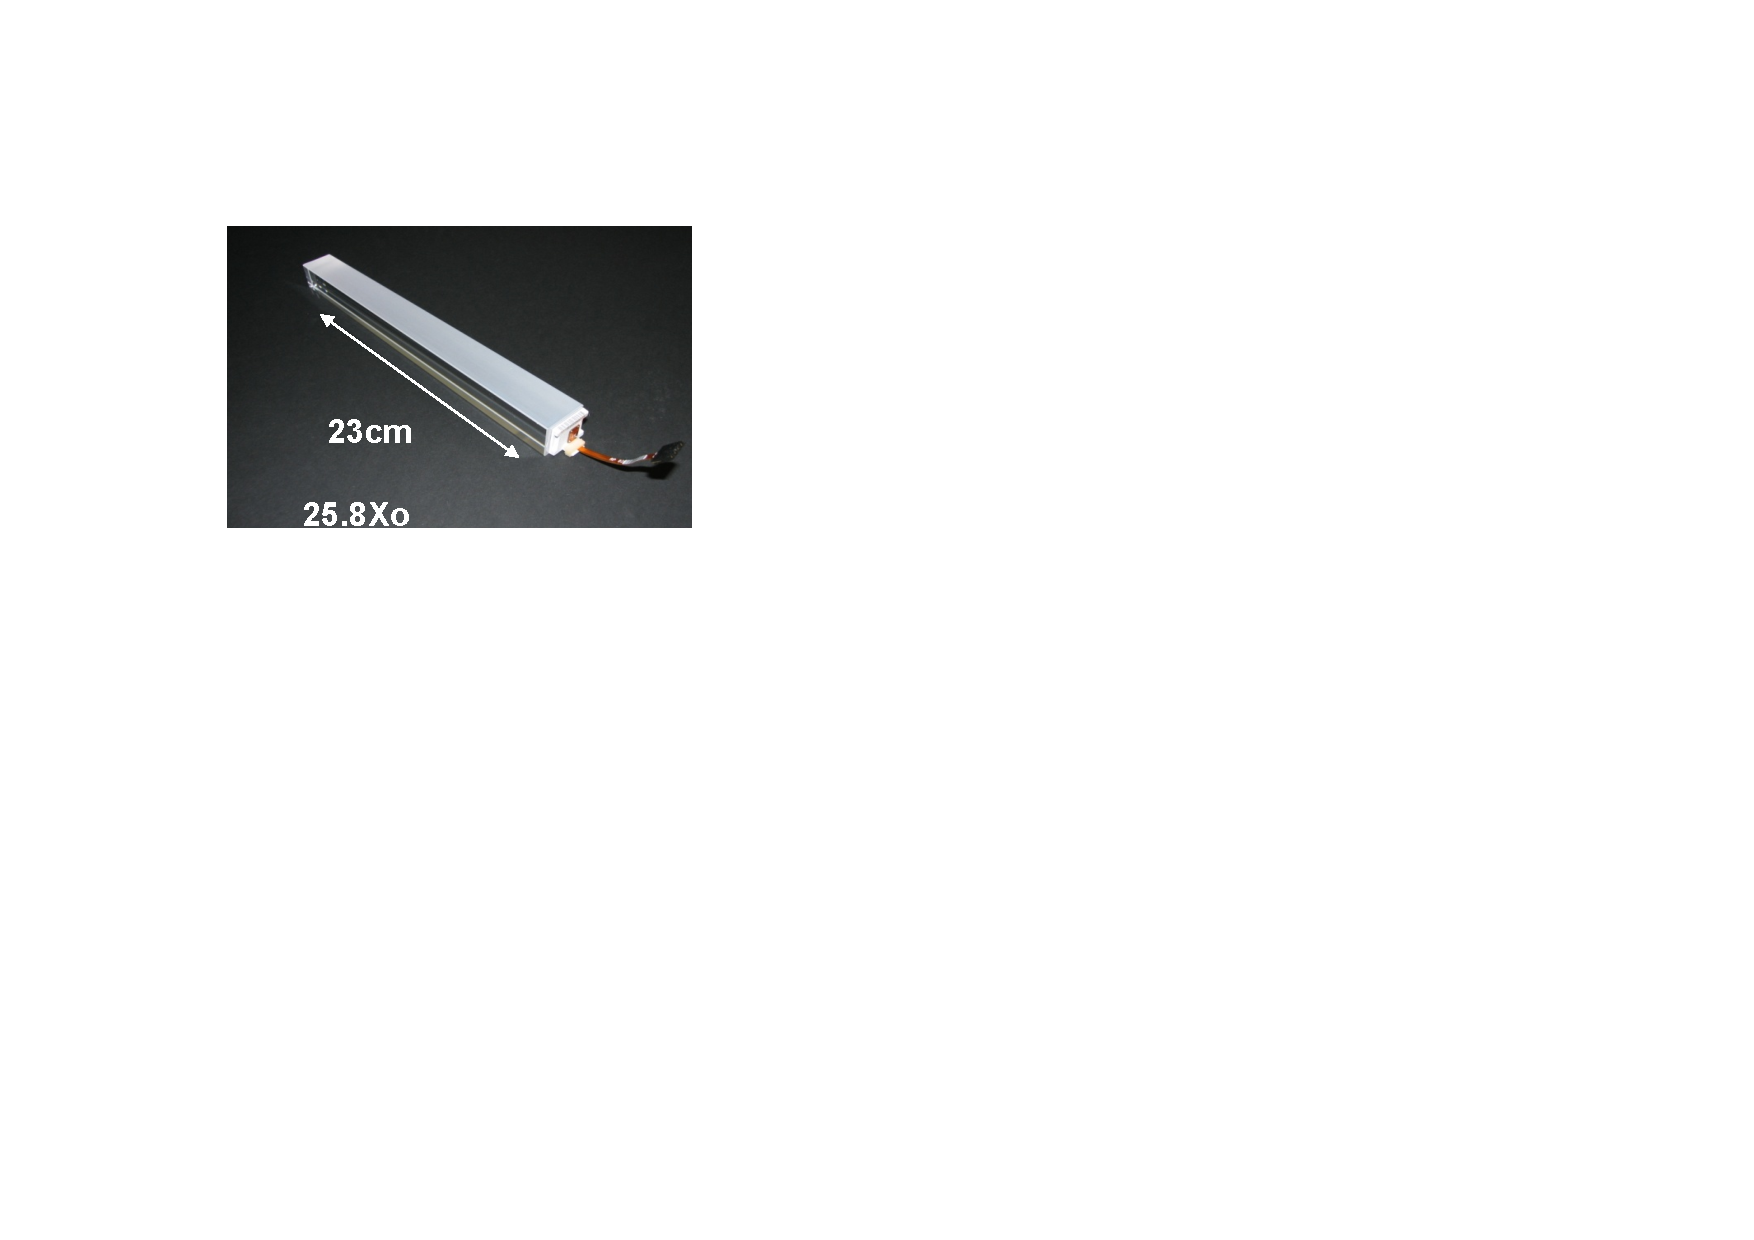
\includegraphics[width=0.45\textwidth]{figures/ecal_crystal_eb}\hfil
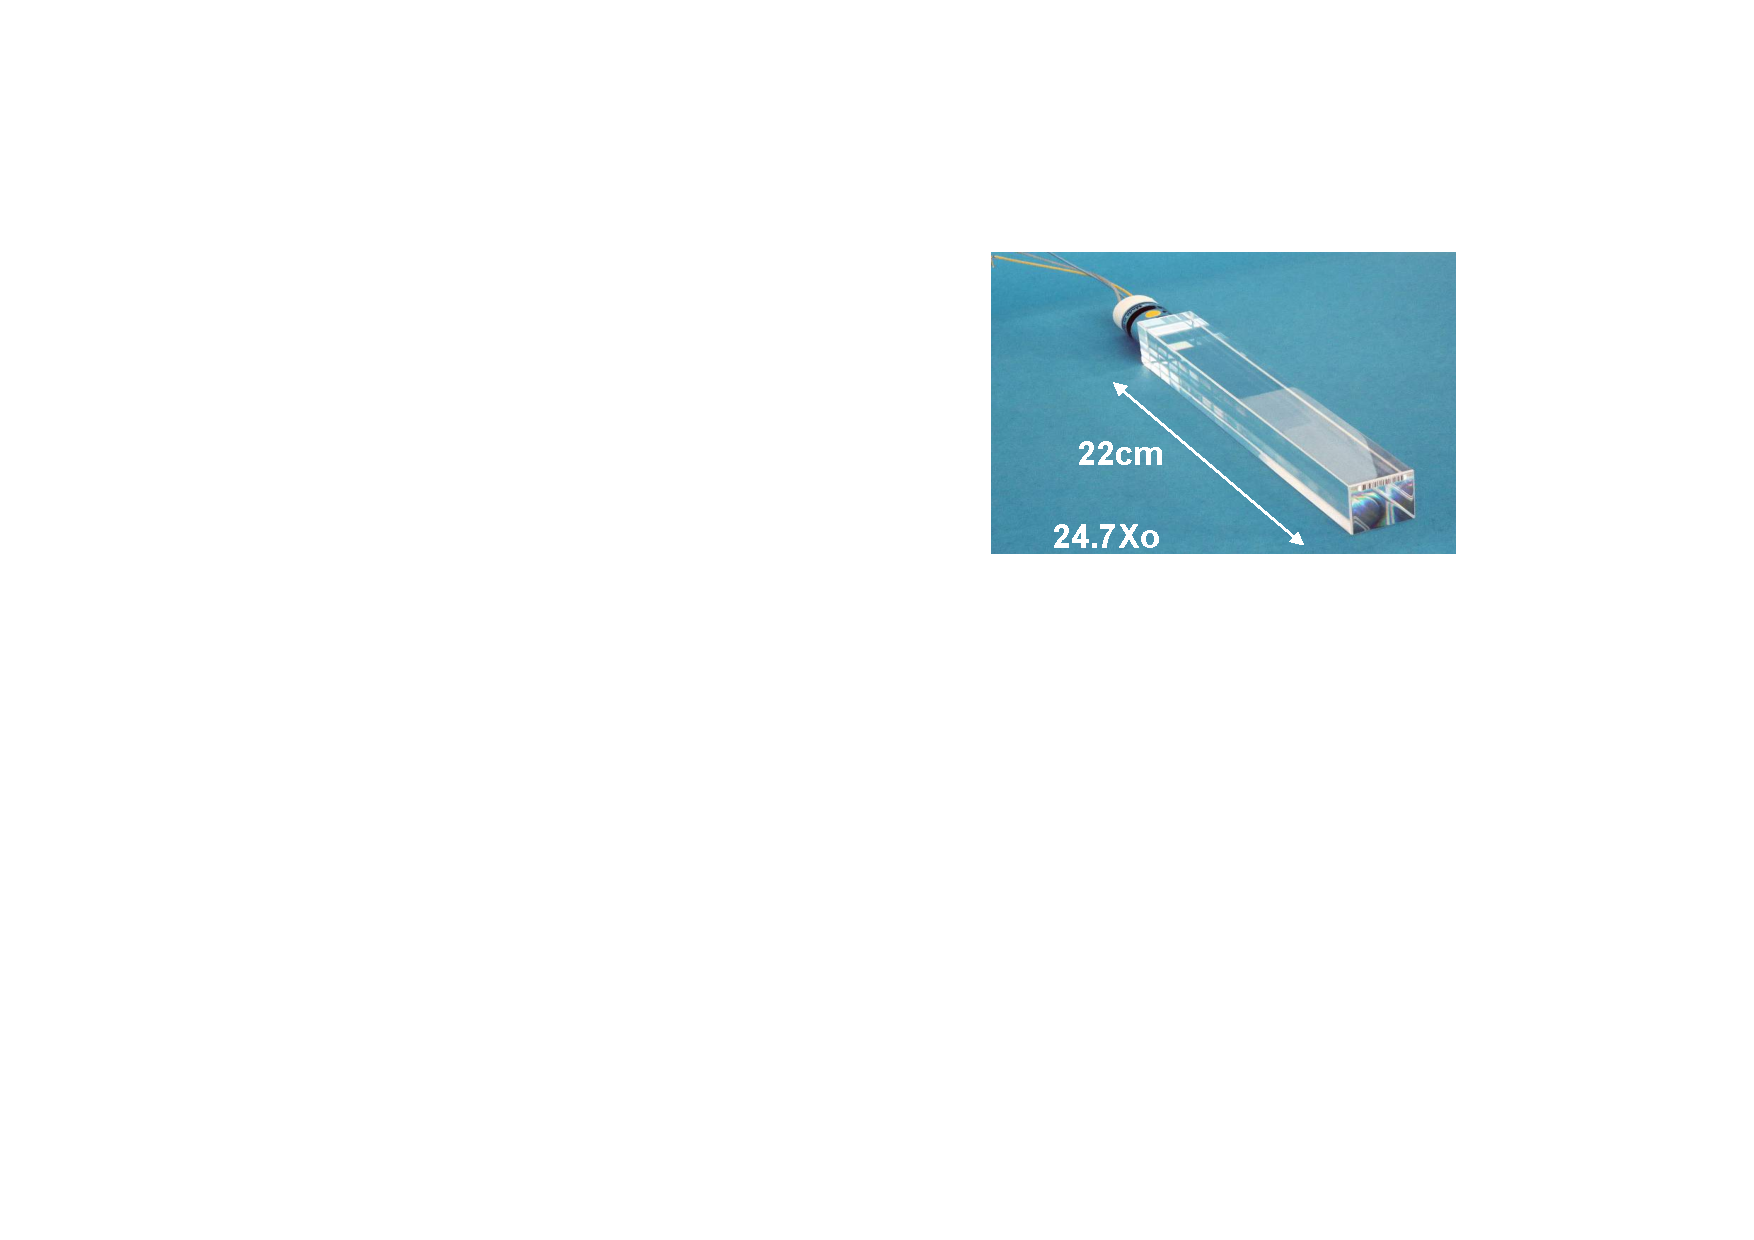
\includegraphics[width=0.45\textwidth]{figures/ecal_crystal_ee}\hfil
\caption{Example of lead tungstate crystals as present on the ECAL barrel (left) and on the ECAL endcap (right). }
\label{fig:ecal_crystals}
\end{figure*}


The ECAL crystals are arranged to provide an off-pointing, pseudo-projective geometry (the crystal axes are tilted at $3^{o}$ with respect to the line from the nominal vertex position), shown in the left of Figure \ref{fig:ecal_geometry}. 
In the barrel, the crystals are mounted in submodules ($2\times5$ crystals in $\phi\times\eta$), which are then mounted into modules and grouped into supermodules. 
Each supermodule contains 4 modules, three with $10\times4$ submodules in $\phi\times\eta$ and one with $10\times5$. An ECAL supermodule is shown on the right of Figure \ref{fig:ecal_geometry}. 

\begin{figure*}[h]
\centering 
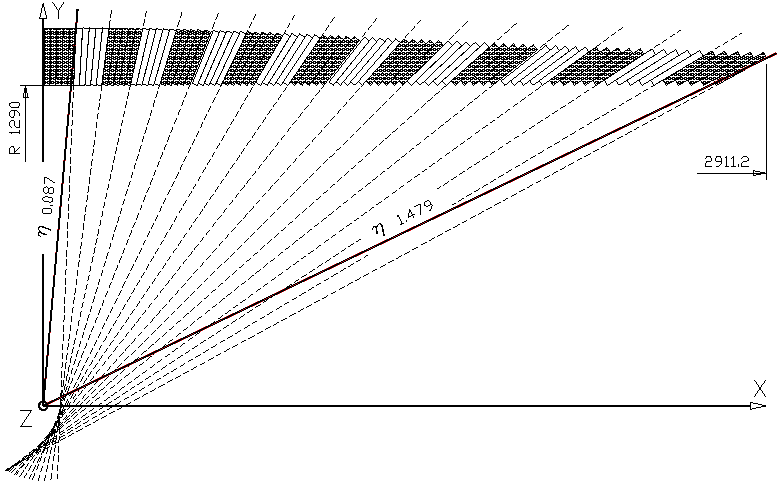
\includegraphics[width=0.45\textwidth]{figures/geometry_barrel}\hfil
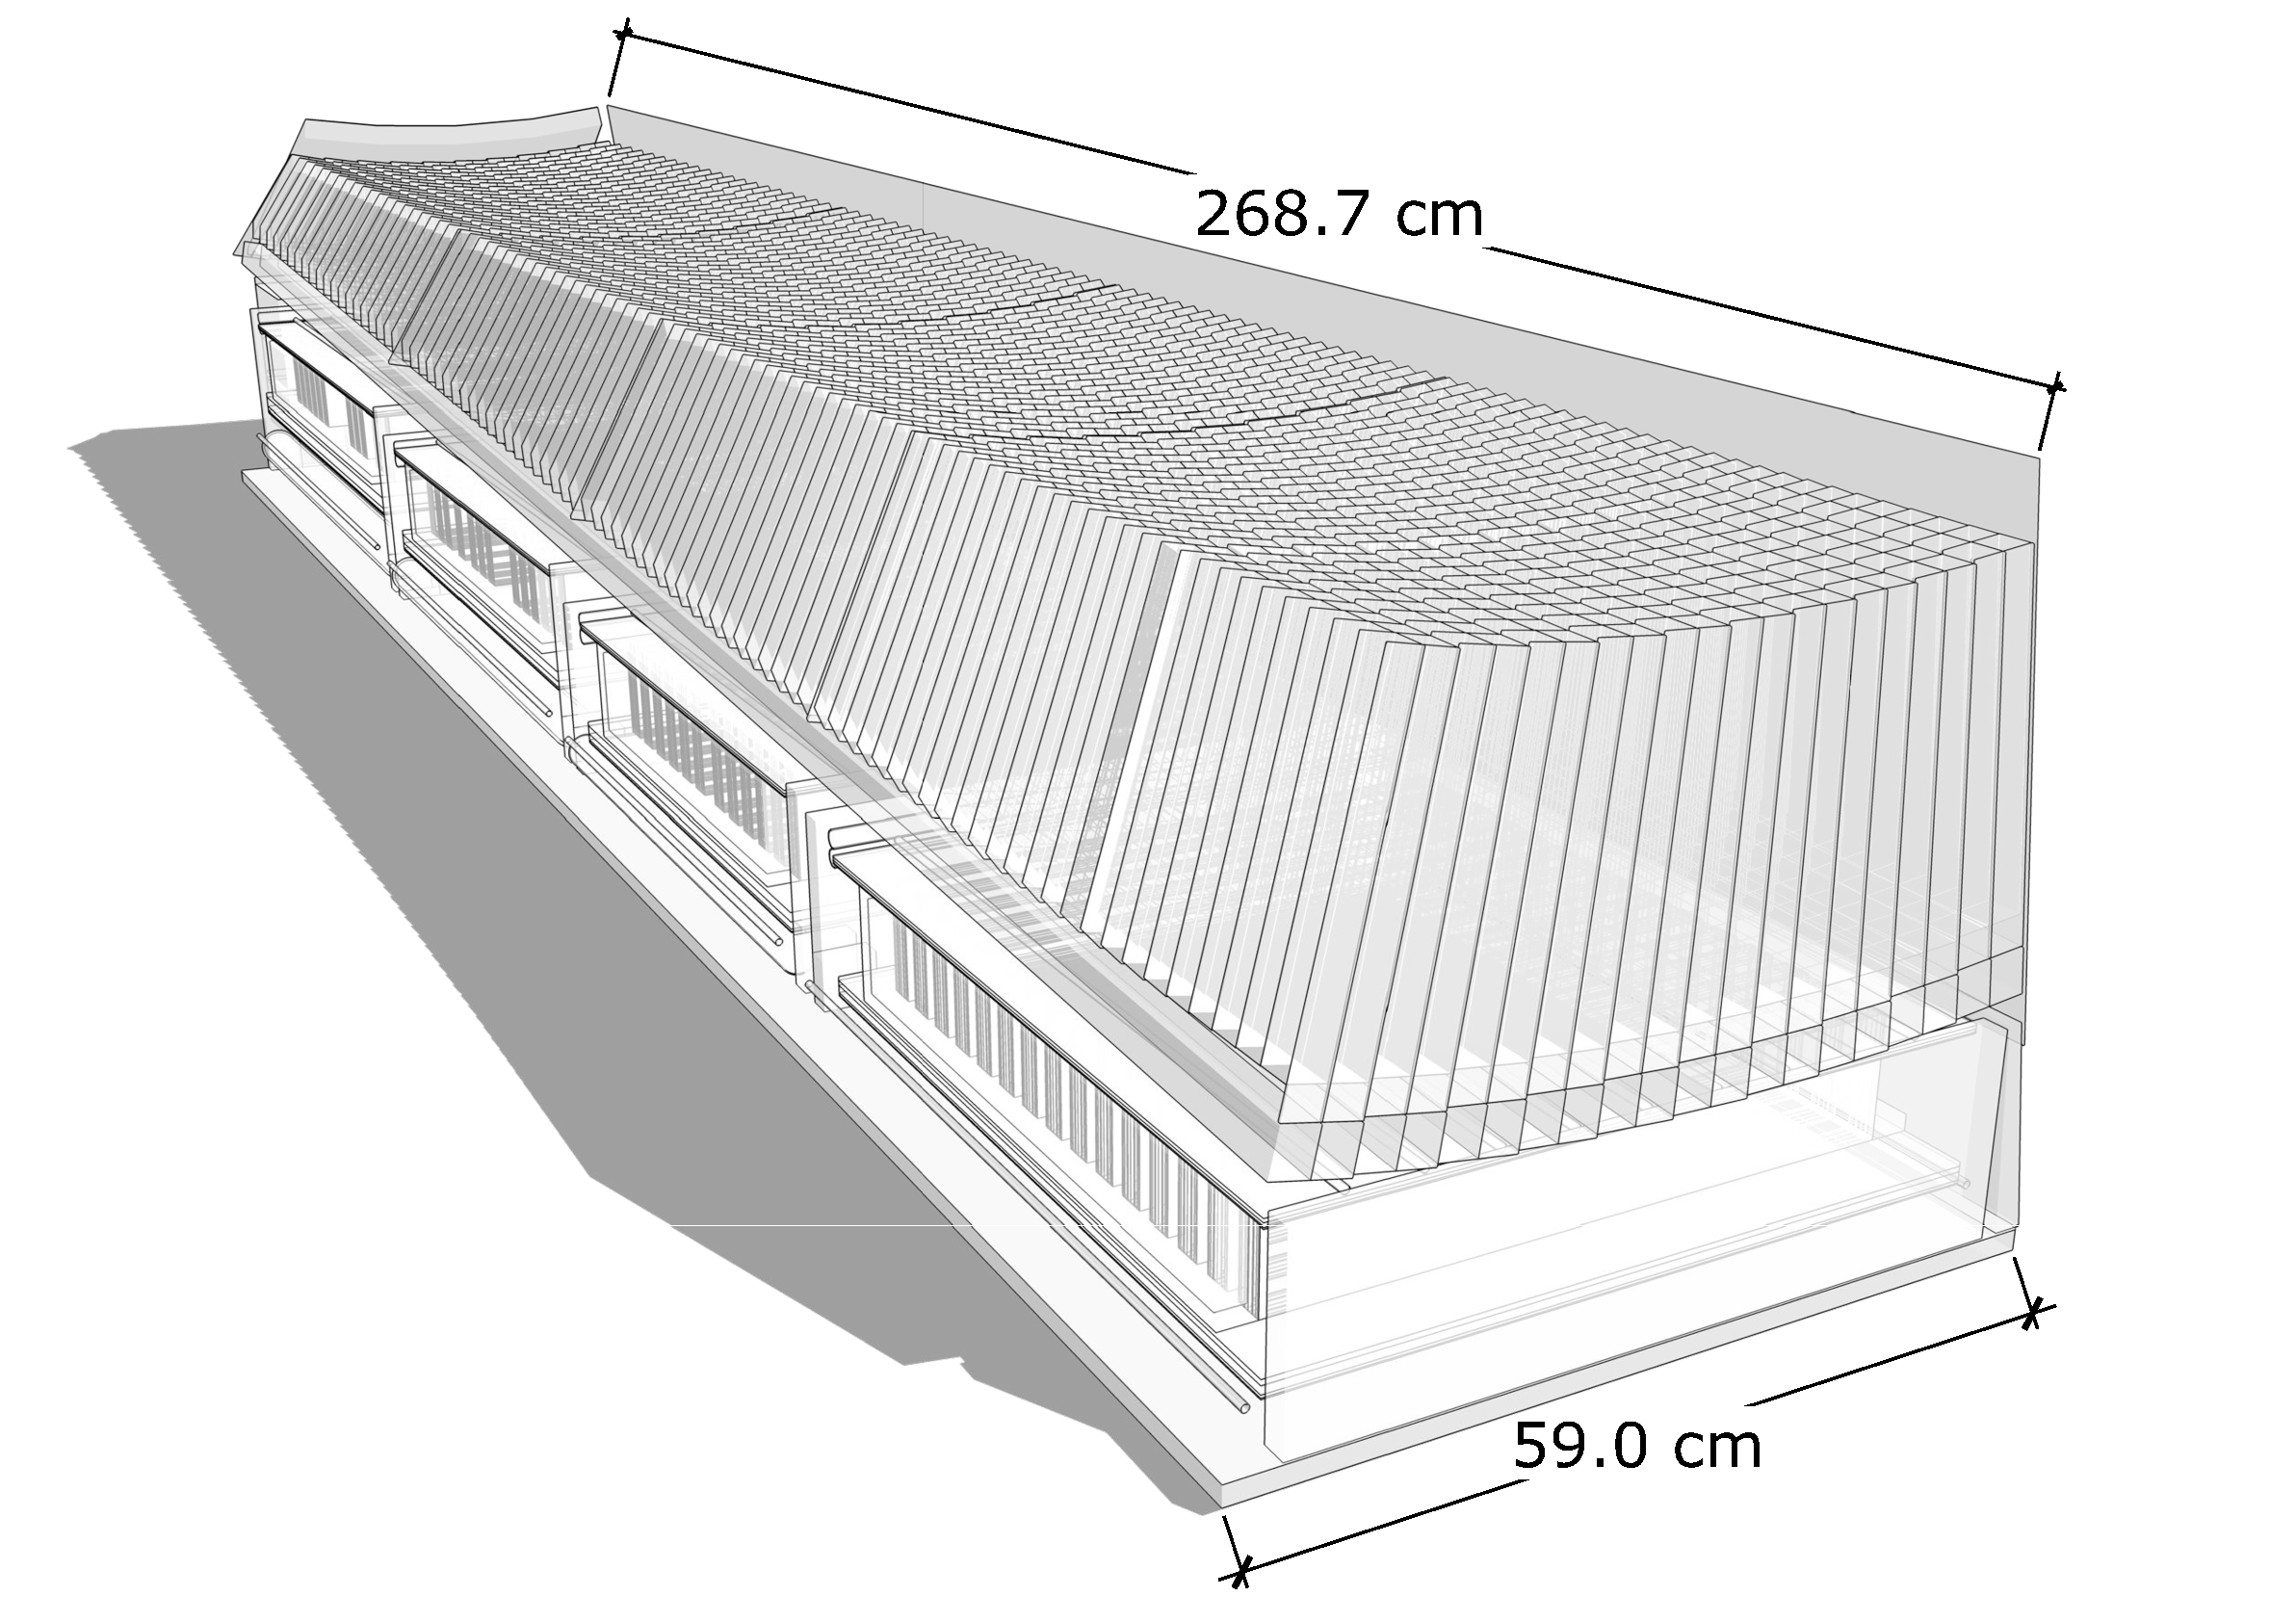
\includegraphics[width=0.45\textwidth]{figures/supermodule}\hfil
\caption{On the left, the CMS ECAL scheme highlighting a barrel supermodule (green), the ECAL endcaps (blue) and the ECAL preshower (red). On the right, the details of a barrel supermodule structure. }
\label{fig:ecal_geometry}
\end{figure*}

An energy deposit is measured in the crystal through a scintillation process, in which the lattice atoms are excited and de-excite by the emission of photons. 
The emission scintillation peak for the ECAL crystals is at about $425$ nm, with $80\%$ of the light emission happening within 25 ns. 
The PbWO$_4$ crystals are also characterized by a small radiation length ($X_{0} = 0.89$ cm), the mean length of that path that takes a high energy electron to lose $(1 - 1/e)$ of its energy in that medium, and a small Moli�re radius ($R_{M} = 2.19$ cm), the radius of a cylinder that contains $90\%$ of the shower energy. 

On the other hand, the ECAL crystals have a low light output yield (about 10 photo-electrons per MeV), and therefore must be coupled to high gain light detectors. 
These detectors must also be radiation hard, to cope with the LHC environment, and be stable under a 4T magnetic field (the CMS solenoid magnet). 
For the ECAL barrel, avalanche photodiodes (APDs) were chosen due to their high gain (50), despite their temperature dependence, which requires ECAL to have a temperature control with a precision better than $0.1^{o}$C (the PbWO$_4$ crystals light yield is also dependent on temperature, with lower light yields for lower temperatures). 
The ECAL APDs are also characterized by their fast, 2 ns rise time, which allows time measurement with the crystals scintillation pulse shape. 
By the time of the ECAL construction, APDs were generally produced in small sizes in comparison to the crystal's rear side area, where they must be attached. For this, two APDs were used for each crystal. 
On the endcaps, the radiation dose incoming is much higher than in the barrel, which does not allow the usage of APDs in the high $\eta$ region. For this reason, vacuum photo-triodes (VPTs) are used instead. While more resistant to radiation, these light detectors have generally a smaller gain (8-10).

\section{Trigger and Data Acquisition Systems}

The ECAL trigger and data acquisition system (Trigger and DAQ) takes care of the the entire data flow from the crystals to the central CMS Trigger and DAQ systems, a schematic version of the system is shown in Figure \ref{fig:ecal_daq}. 

\begin{figure*}[h]
\centering 
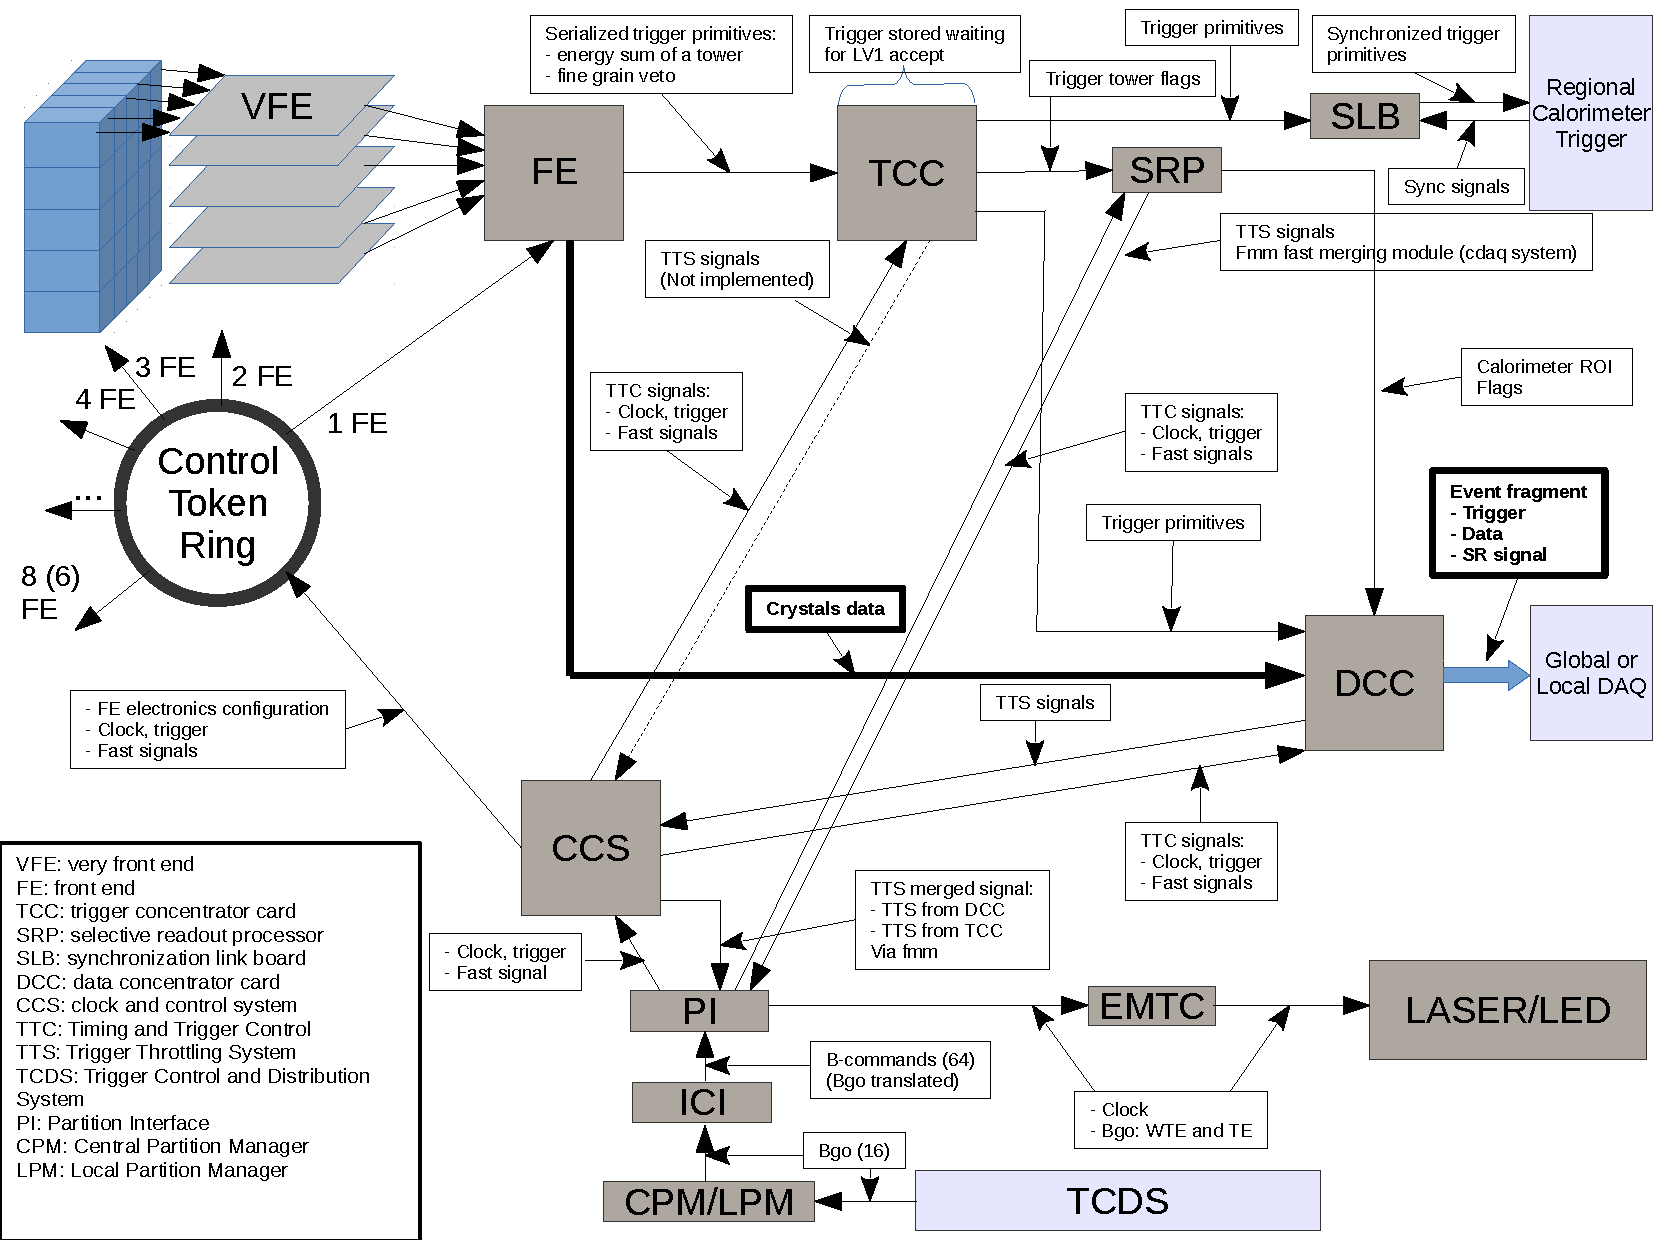
\includegraphics[width=0.7\textwidth]{figures/ecal_daq}\hfil
\caption{ECAL DAQ simplified scheme. }
\label{fig:ecal_daq}
\end{figure*}

\subsection{Data Flow}

The ECAL data flow starts right after the signal is detected by the photo detectors attached to the crystals. 
The first step in the chain is the amplification and digitization of the analog signal coming from the APDs and VPTs. 
This is performed with multi-gain pre-amplifiers (MGPAs). 
The ECAL MGPAs work with amplification gains: gain-12, gain-6 and gain-1. 
The shaping time associated with this amplification process is of about 40 ns. 
The signal is then sampled and digitized at a rate of 40 MHz. 
One pulse shape is then reconstructed using 10 of these samples. 
The electronics responsible for the amplification and digitization step is generally called very-front-end electronics (VFE). 


The VFE sends information to the front-end electronics (FE) at the sampling rate. 
The FE is responsible for creating trigger primitives, basic information such as energy and position, from arrays of $5\times5$ crystals (trigger towers). 
The trigger primitives are sent from the FE to the trigger concentrator cards (TCCs) at sampling rate, and passed to the CMS Level-1 trigger (L1A signal). 
The VFE and the FE, known as the in-detector electronics, are placed right at the detector, close to the crystals, which is schematically shown in Figure \ref{fig:ecal_vfe}. 
In Figure \ref{fig:ecal_vfe}, the chips dedicated to generating and transmitting the serialized trigger primitives (FENIX chips) are shown, along with the gigabit optical hybrids (GOH) chips dedicated to data transmission and the chips dedicated to receiving and distributing timing and control data (CCU). 

\begin{figure*}[h]
\centering 
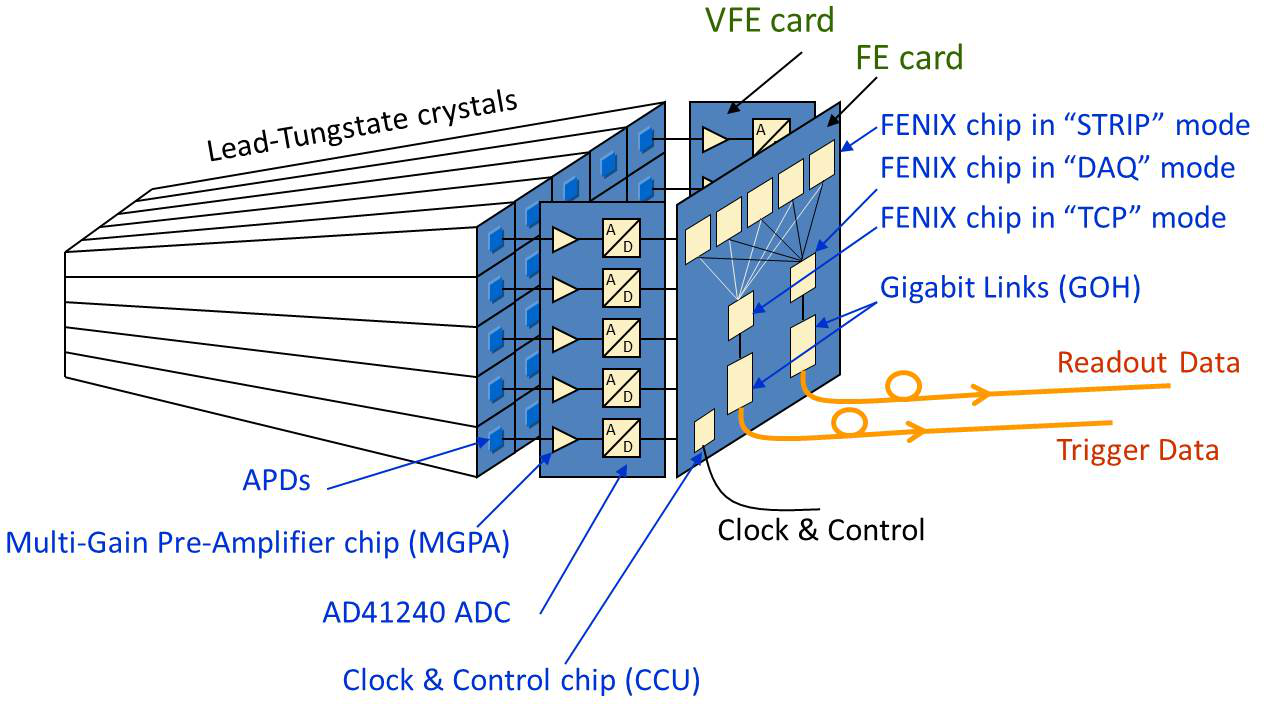
\includegraphics[width=0.7\textwidth]{figures/ecal_vfe}\hfil
\caption{ECAL in-detector electronics simplified scheme. }
\label{fig:ecal_vfe}
\end{figure*}

During the time it takes for a decision to be made by the L1 trigger, the trigger primitives are stored at the TCCs. 
In case the event is not accepted, these trigger primitives and the full crystal information stored at the FE are flushed from memory. 
If an event is accepted, the FE sends the serialized full individual crystals information to the data concentrator cards (DCCs), that will pack the event in a format readable by the CMS central DAQ. 

In parallel, the TCC sends the trigger primitive information to the selective readout units (SRPs) after an L1A arrives. 
The SRP selects which portions of the detector should be unpacked by the DCCs based on an algorithm called Selective Readout (SR), reducing the load of processing by the DCCs. 
The DCCs load is limited by the current electronics architecture and can be trespassed when the average activity per event is increased, such as in high pile up LHC runs.  
The SR algorithm classifies trigger towers as low interest ($E_{TT} < 1.5$ GeV), medium interest ($1.5 < E_{TT} < 2.5 $ GeV) or high interest ($E_{TT} > 2.5$ GeV). 
If a trigger tower is classified as low interest, only the crystals with energy higher than 4.5 (6.5) ADC in the barrel (endcap). 
If a trigger tower is classified as medium interest, all crystals are unpacked, regardless of their energies. 
If a trigger tower is classified as high interest, all crystals in that trigger tower, and the 8 trigger towers around it are fully read.

\subsection{Timing and Control Distribution}

In order to ensure a synchronized working of all different parts of the ECAL DAQ system, a precise distribution of clock and control signals must be achieved. 
This is performed via a combination of different ECAL and central CMS electronics. 
For Run 2, CMS installed a new subsystem dedicated to distributing these signals among all CMS partitions, the Timing and Control Distribution System (TCDS). 
TCDS communicates timing/synchronization signals coming from the LHC and CMS (clock), L1As coming from the CMS Level-1 trigger, and configuration and control commands synchronously to all CMS components. 
These signals are then distributed among ECAL components via the clock and control system (CCS), including to the front-end electronics (through control token rings). 

\subsubsection{TCDS}

The TCDS subsystem was installed on CMS during the Long Shutdown 1 in order to cope with the new running conditions for Run 2. 
Specifically, new detector subsystems were being installed in the experiment (such as the new pixel inner tracker layers). 
Instead of expanding the old system, a choice was made to construct a new infrastructure with updated hardware, firmware and software. 
The TCDS system consists on three types of boards: the Central Partition Manager (CPM), the CMS Interface boards (iCI) and the Partition Interface boards (PI). 

The TCDS CPM is fully controlled by the central TCDS system, and has information regarding the type of runs to be started by the central DAQ. 
This information defines, for example, at which point of the LHC orbit to send specific signals to the subdetectors. 
The iCIs must work as a library that translates the CPM signals into specific actions to be taken by the different subdetectors. This means that the iCIs must be configured properly and individually by each subdetector. 
In order to achieve that on ECAL, a new software interface to TCDS was written to configure and monitor the ECAL iCIs. 
The PIs act as fan-out boards to distribute the iCI messages among different subdetector components.

\subsection{Software Architecture}

The ECAL DAQ software architecture controls, configures and monitors the readout and trigger electronics described in the previous sections. 
The framework implementation is based on a CMS common framework developed by the central Trigger and DAQ group, mostly consisting of  C++ xDAQ framework \cite{xdaq}, while the top layer of the system is based on the JAVA RCMS \cite{rcms} framework.

The overall system accomplishes several different tasks. It configures and monitors the different components of the FE and and off-detector electronics. 
It communicates with the central CMS TCDS, both sending the correct configuration parameters for the dedicated TCDS ECAL boards and receiving and translating these commands to the off-detector electronics. 
It is also able to perform different types of runs dedicated to calibration and detector developments, such as "MiniDAQ" and "local" runs.

With the xDAQ framework, the ECAL software communicates to the ECAL boards through SOAP (Simple Object Access Protocol) messages. 
SOAP messages are also used to communicate issues with the off-detector electronics directly to the central DAQ system. 

There are five main components to the ECAL DAQ software architecture:
\begin{description}
\item[ECAL Function Manager] Function managers (FM) work as the overall controller of actions happening to the ECAL software. It has the power to send commands to the ECAL supervisor to cause state transitions, triggering actions such as the beginning of a run. During global CMS runs, the central DAQ function communicates such actions to the ECAL function manager. In specific runs in which ECAL controls its own sequence, the ECAL function manager works by itself.
\item[ECAL Supervisor] The ECAL supervisor is at the top of software control and coordinates all other working pieces. It receives the commands from the ECAL function manager and, to any given command, proceeds with the specific steps to ensure the state transitions of the different com ECAL components.
\item[Services Supervisors] For each different services described in the previous sections (TCC, DCC, DCS and SRP), a dedicated software exists in order to perform the actions related to specific state transitions.
\item[TCDS Supervisor] A specific supervisor was developed to communicate with the central TCDS service. It sends the proper configuration parameters to the TCDS ECAL boards, with the list of commands to be passed to the ECAL electronics when certain state transitions happen and during specific run conditions.
\item[Monitoring Services] In order to retrieve and display information about the status of the off-detector electronics, specific services based on xDAQ capabilities are used. These services also monitor the ECAL DAQ computing capabilities to make sure all machines are working properly. Depending on what type of error is detected by the monitoring services, SMS's and e-mails are sent to ECAL DAQ experts.
\end{description}

\subsubsection{ECAL DAQ Finite State Machine}

One of the main goals of the ECAL Supervisor is to ensure the proper state transitions of the different DAQ components through the allowed states of the ECAL DAQ Finite State Machine (FSM), summarized in Figure \ref{fig:ecal_fsm}.

\begin{figure*}[h]
\centering 
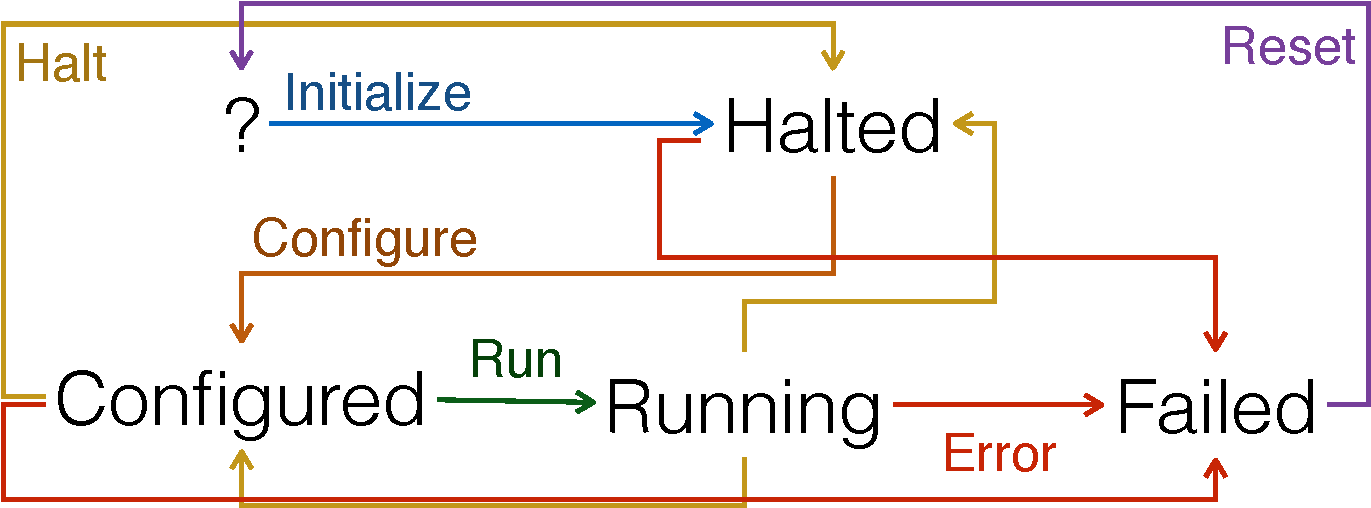
\includegraphics[width=0.7\textwidth]{figures/ecal_fsm}\hfil
\caption{Simplified view of the ECAL Finite State Machine and its transitions. }
\label{fig:ecal_fsm}
\end{figure*}

 
Similarly to the central CMS FSM, the transitions are: 

\begin{description}
\item[Initialization] The Initialization procedure tests the connection between the ECAL Supervisor and the different off-detector components and initializes all required drivers. The information about the hardware resources is then propagated back to the supervisor and the ECAL FM. The initialization transition takes the FSM to Halted state and makes it ready to be configured.
\item[Configuration] When the configuration signal is received, it reads the configuration parameters from the ECAL Configurations DataBase (ConfDB) and sends to the off-detector electronics, which are then loaded accordingly. Each different Service Supervisor independently ensures their components have been successfully configured and communicate it back to the ECAL Supervisor. This action takes the FSM to Configured state and is now ready to start producing data (running). It also enables the monitoring services. 
\item[Start] The start command kicks-off the full data flow described at the beginning of this section, including trigger primitive production and delivery to the L1 trigger, and the delivery of the full data information upon an L1A. It also starts the delivery of monitoring data from the off-detector electronics to the monitoring services. This action takes the FSM to Running state.
\item[Stop/Halt] These actions take the system either from Running state to Configured state, or from Running or Configured states to Halted state, respectively. The Stop command  interrupts the ECAL DAQ data flow, while the the Halt command interrupts the data flow and flushes the database parameters from the off-detector electronics. 
\item[Error] Any error during the previous transitions will take the FSM to Failed state.
\end{description}

\subsubsection{Types of Running Conditions with the ECAL}

\begin{description}
\item[Global Runs] A global run is the usual working condition of ECAL with the full CMS central DAQ infrastructure. In global runs, the ECAL FM receives commands directly from the central DAQ FM, including all state transition actions. These runs happen when the LHC is running, when CMS is taking cosmics data (with its magnetic field on or off) or when specific tests must be performed with the full central DAQ infrastructure. 
\item[MiniDAQ Runs] These runs happen with a dedicated central DAQ infrastructure that is independent of global runs, and therefore can run in parallel. They are used on ECAL to test the state of the off-detector electronics and investigate possible errors seen in global runs. MiniDAQ runs have also been used in 2015 and 2016 to measure the response of the ECAL electronics to noise (pedestals) and to test pulses generated by the on-detector electronics.
\item[Local Runs] Local runs are completely independent from the central DAQ infrastructure. They rely on ECAL software to both directly configure the off-detector electronics and process the data that is produced by the DCCs. This freedom allows for more complex types of running conditions, such as the ones needed for more coherent measurements of ECAL pedestals (to be used in 2017).
\end{description}


\section{Electron and Photon Energy Reconstruction}

The photon and electron energy reconstruction based on ECAL energy deposits is based on the formula: 
\begin{equation}
E_{e,\gamma} = \left[ \sum_{i}\left( S_i(t)\times c_{i} \times A_{i}\right)\times G(\eta) + E_{ES} \right]\times F_{e,\gamma},
\end{equation}
 with $A_{i}$, $c_i$ and $S_i(t)$ as, respectively, the per individual channel amplitude, intercalibration constant and light monitoring constant, $G(\eta)$ is the ADC to GeV absolute scale, $E_{ES}$ is the energy deposit in the preshower, and $F_{e,\gamma}$ are the cluster corrections (different for photons and electrons). The methods used to obtain the different terms in this equation will be detailed in the next sections. 

\subsection{Online Reconstruction}

%The online reconstruction of ECAL deposits starts with the amplification and digitization of the signal from the photodetectors attached to the crystals. This is performed by a multi-gain preamplifier (MGPA), and a 12 bit ADC running at 40 MHz. Ten consecutive samples are recorded and used to perform the pulse reconstruction and amplitude extraction.

The time spacing between two consecutive samples from the ECAL readout electronics is 25 ns, which is the same time spacing between two colliding bunches in the LHC. 
This implies that, during the readout of one pulse, another scintillation process might start in the same crystal, compromising the in-time amplitude reconstruction. 
To mitigate this effect, also called out-of-time (OOT) pile up, a new online pulse reconstruction method (multifit) was developed to replace the Run I method \cite{weights}.

\begin{figure*}[h]
\centering 
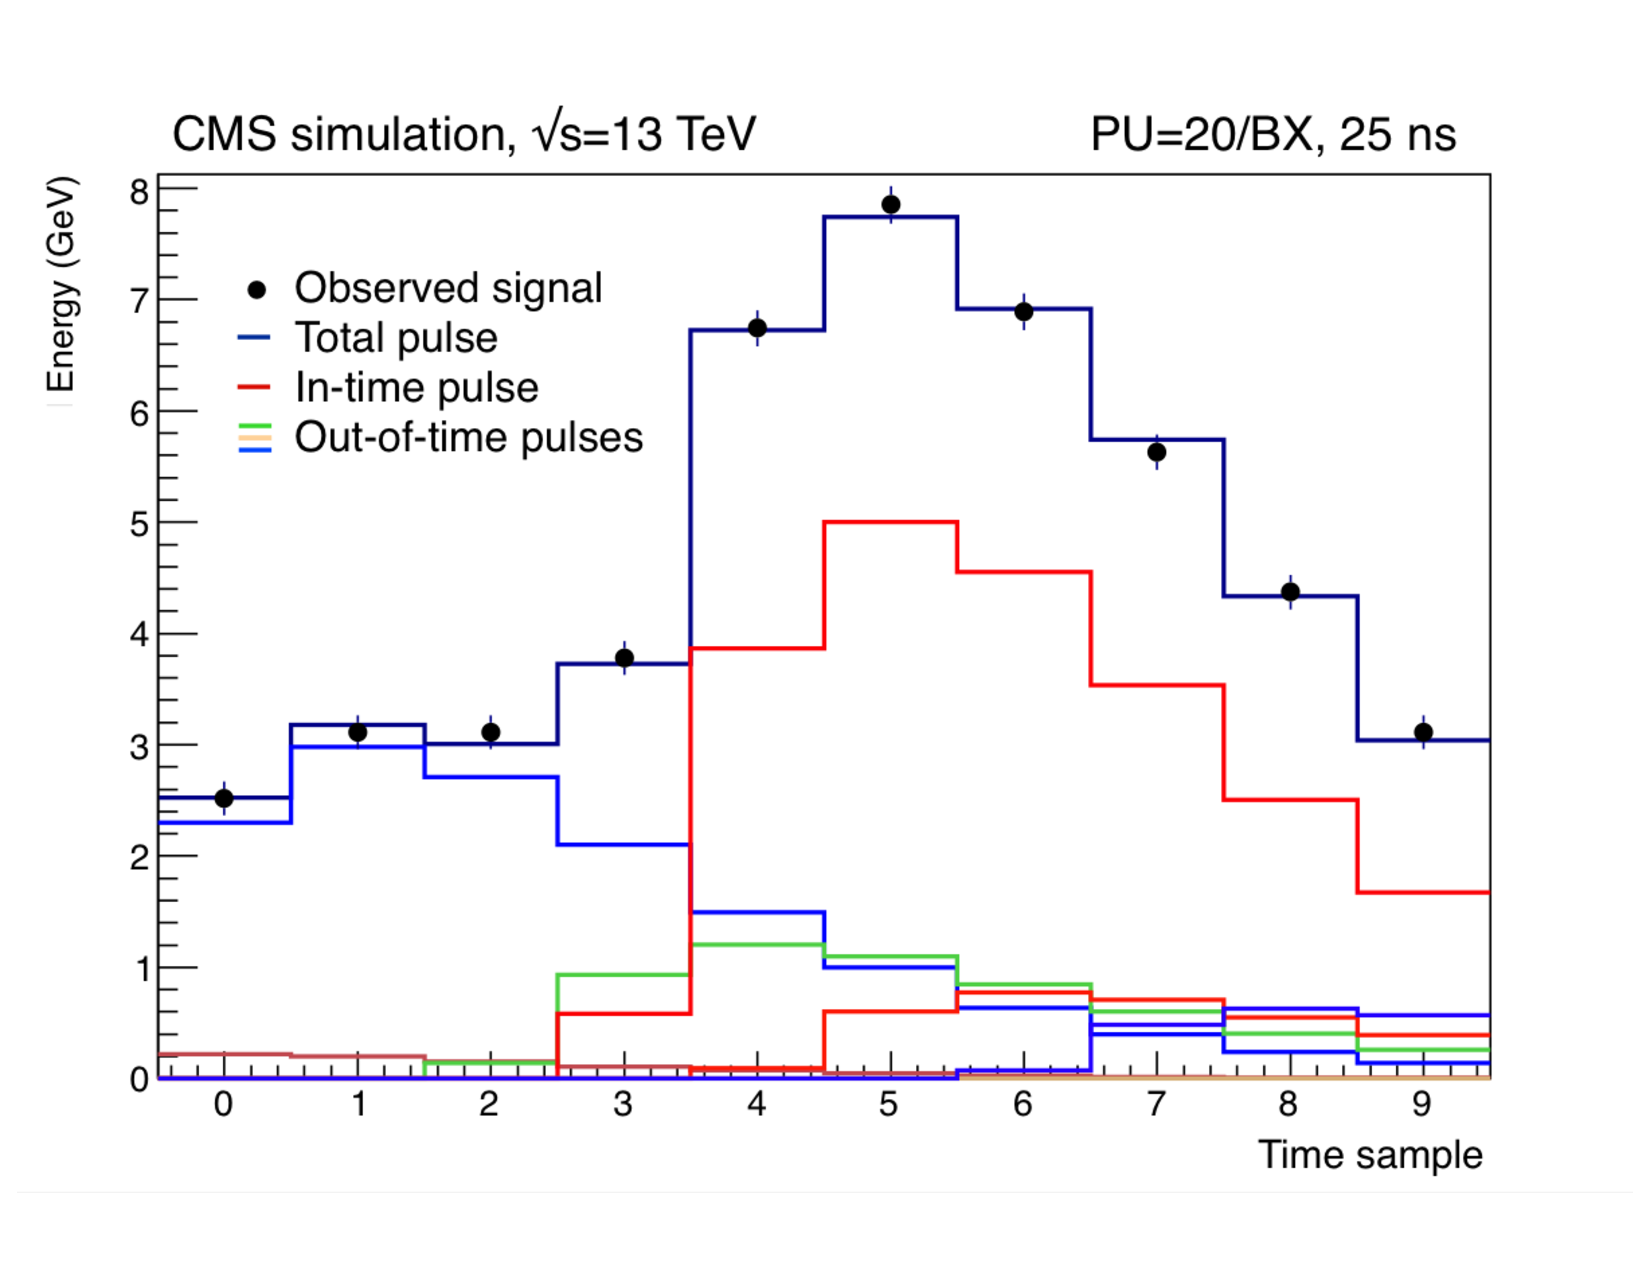
\includegraphics[width=0.45\textwidth]{figures/multifit_pulses}\hfil
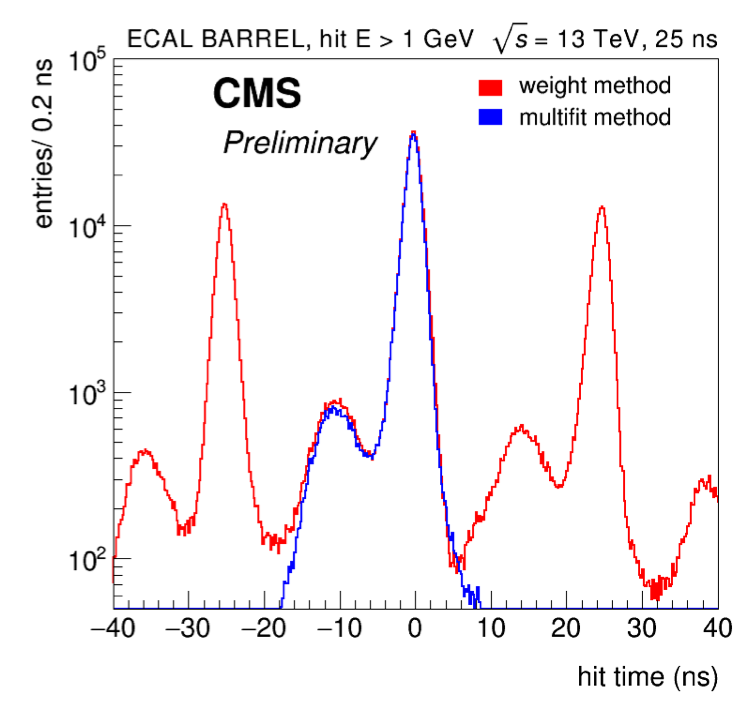
\includegraphics[width=0.45\textwidth]{figures/multifit_oot}\hfil
\caption{(Left) Fitted pulse shapes with the multifit method. (Right) In-time and out-of-time contributions to energy reconstruction with weights method (red) and multifit (blue).}
\label{fig:ecal_daq}
\end{figure*}


In the multifit method, the pulse shape is reconstructed based on a fit to the time samples, minimizing $\chi^2 = \sum_{i=1}^{10}{\left( \sum_j^MA_jp_{ij} - S_i \right)^2}/{\sigma^2_{S_i}}$. The samples ($S_i$) are fitted with one in-time pulse shape template, plus up to 9  out-of-time templates ($p_{ij}$) times their respective amplitudes ($A_j$). $\sigma_{S_i}$ is noise generated by electronics associated with the crystal readout chain. The OOT templates have the same shape as the in time one, but are shifted in time by multiples of 1 bunch crossing (1 BX = 25 ns), within a range of -5 to +4 BX around the in time signal (BX = 0). The pulse shapes have been measured in early 2015, in special runs in which the LHC delivered isolated bunches (no OOT pile up).

It has been observed in both data and simulation that, with the multifit method, OOT pile up reconstruction is negligible. The energy resolution improvement, with respect to the Run I amplitude reconstruction method, is substantial especially for low $E_{T}$ photons and electrons, given the larger contribution of deposits from pile up to the total energy.


\subsection{Response Monitoring}

Time dependent corrections must be applied to the reconstructed amplitude due to changes in detector response with radiation exposure. These changes in response are due to decreases in crystal transparency and variations in VPT response in endcaps.

The changes in the crystal transparency is due to ionizing radiation creating color centers in the lead tungstate. While the scintillation process remains intact, the amount of light detected by the photodetectors decreases. This effect is partially mitigated through thermal annealing, causing the transparency to increase in the absence of radiation.

A light monitoring system is used to monitor the overall changes in response in the ECAL \cite{laser}. It consists of a system of lasers (operating at 447 nm, close to the wavelength of peak emission for lead tungstate) that injects light in each ECAL crystal, which is then read by the standard ECAL readout. The change in transparency per crystal ($R/R_0$) is then related to the ratio between reconstructed amplitude and the injected light amplitude ($S/S_0$) through the formula:

\begin{equation}
\frac{S}{S_0} = \left(\frac{R}{R_0} \right)^{\alpha},
\end{equation}
where $\alpha$ has been measured in beam tests and is $\approx 1.5$. $S/S_0$ is then used as a correction factor to account for the response changes.

The light monitoring infrastructure is an integral part of the ECAL DAQ. 
It works alongside of the main data flow, in specific periods in which the LHC bunches are empty (orbit gaps). 
During the orbit gaps, the laser system is shown in different parts of the ECAL barrel and endcaps. 
In about 40 minutes, one reading of the full ECAL is performed. 

The history of response change measurements is summarized in Figure \ref{fig:fig_laser}. The changes are up to $6\%$ in the barrel and  reach up to $30\%$ at $|\eta| \approx 2.5$, the limit of the tracker acceptance. For high $|\eta|$ regions, changes are up to $70\%$. The recovery of the crystal response during the long shutdown period is visible. The response was not fully recovered, however, particularly in the region closest to the beam pipe. The monitoring corrections are validated by comparing isolated electron energy as measured by ECAL ($E$) and momentum as measured by the CMS Tracker ($p$), before and after light monitoring corrections. It is seen that the measured corrections bring stability to energy measurements with ECAL.

\begin{figure*}[tbh]
\centering 
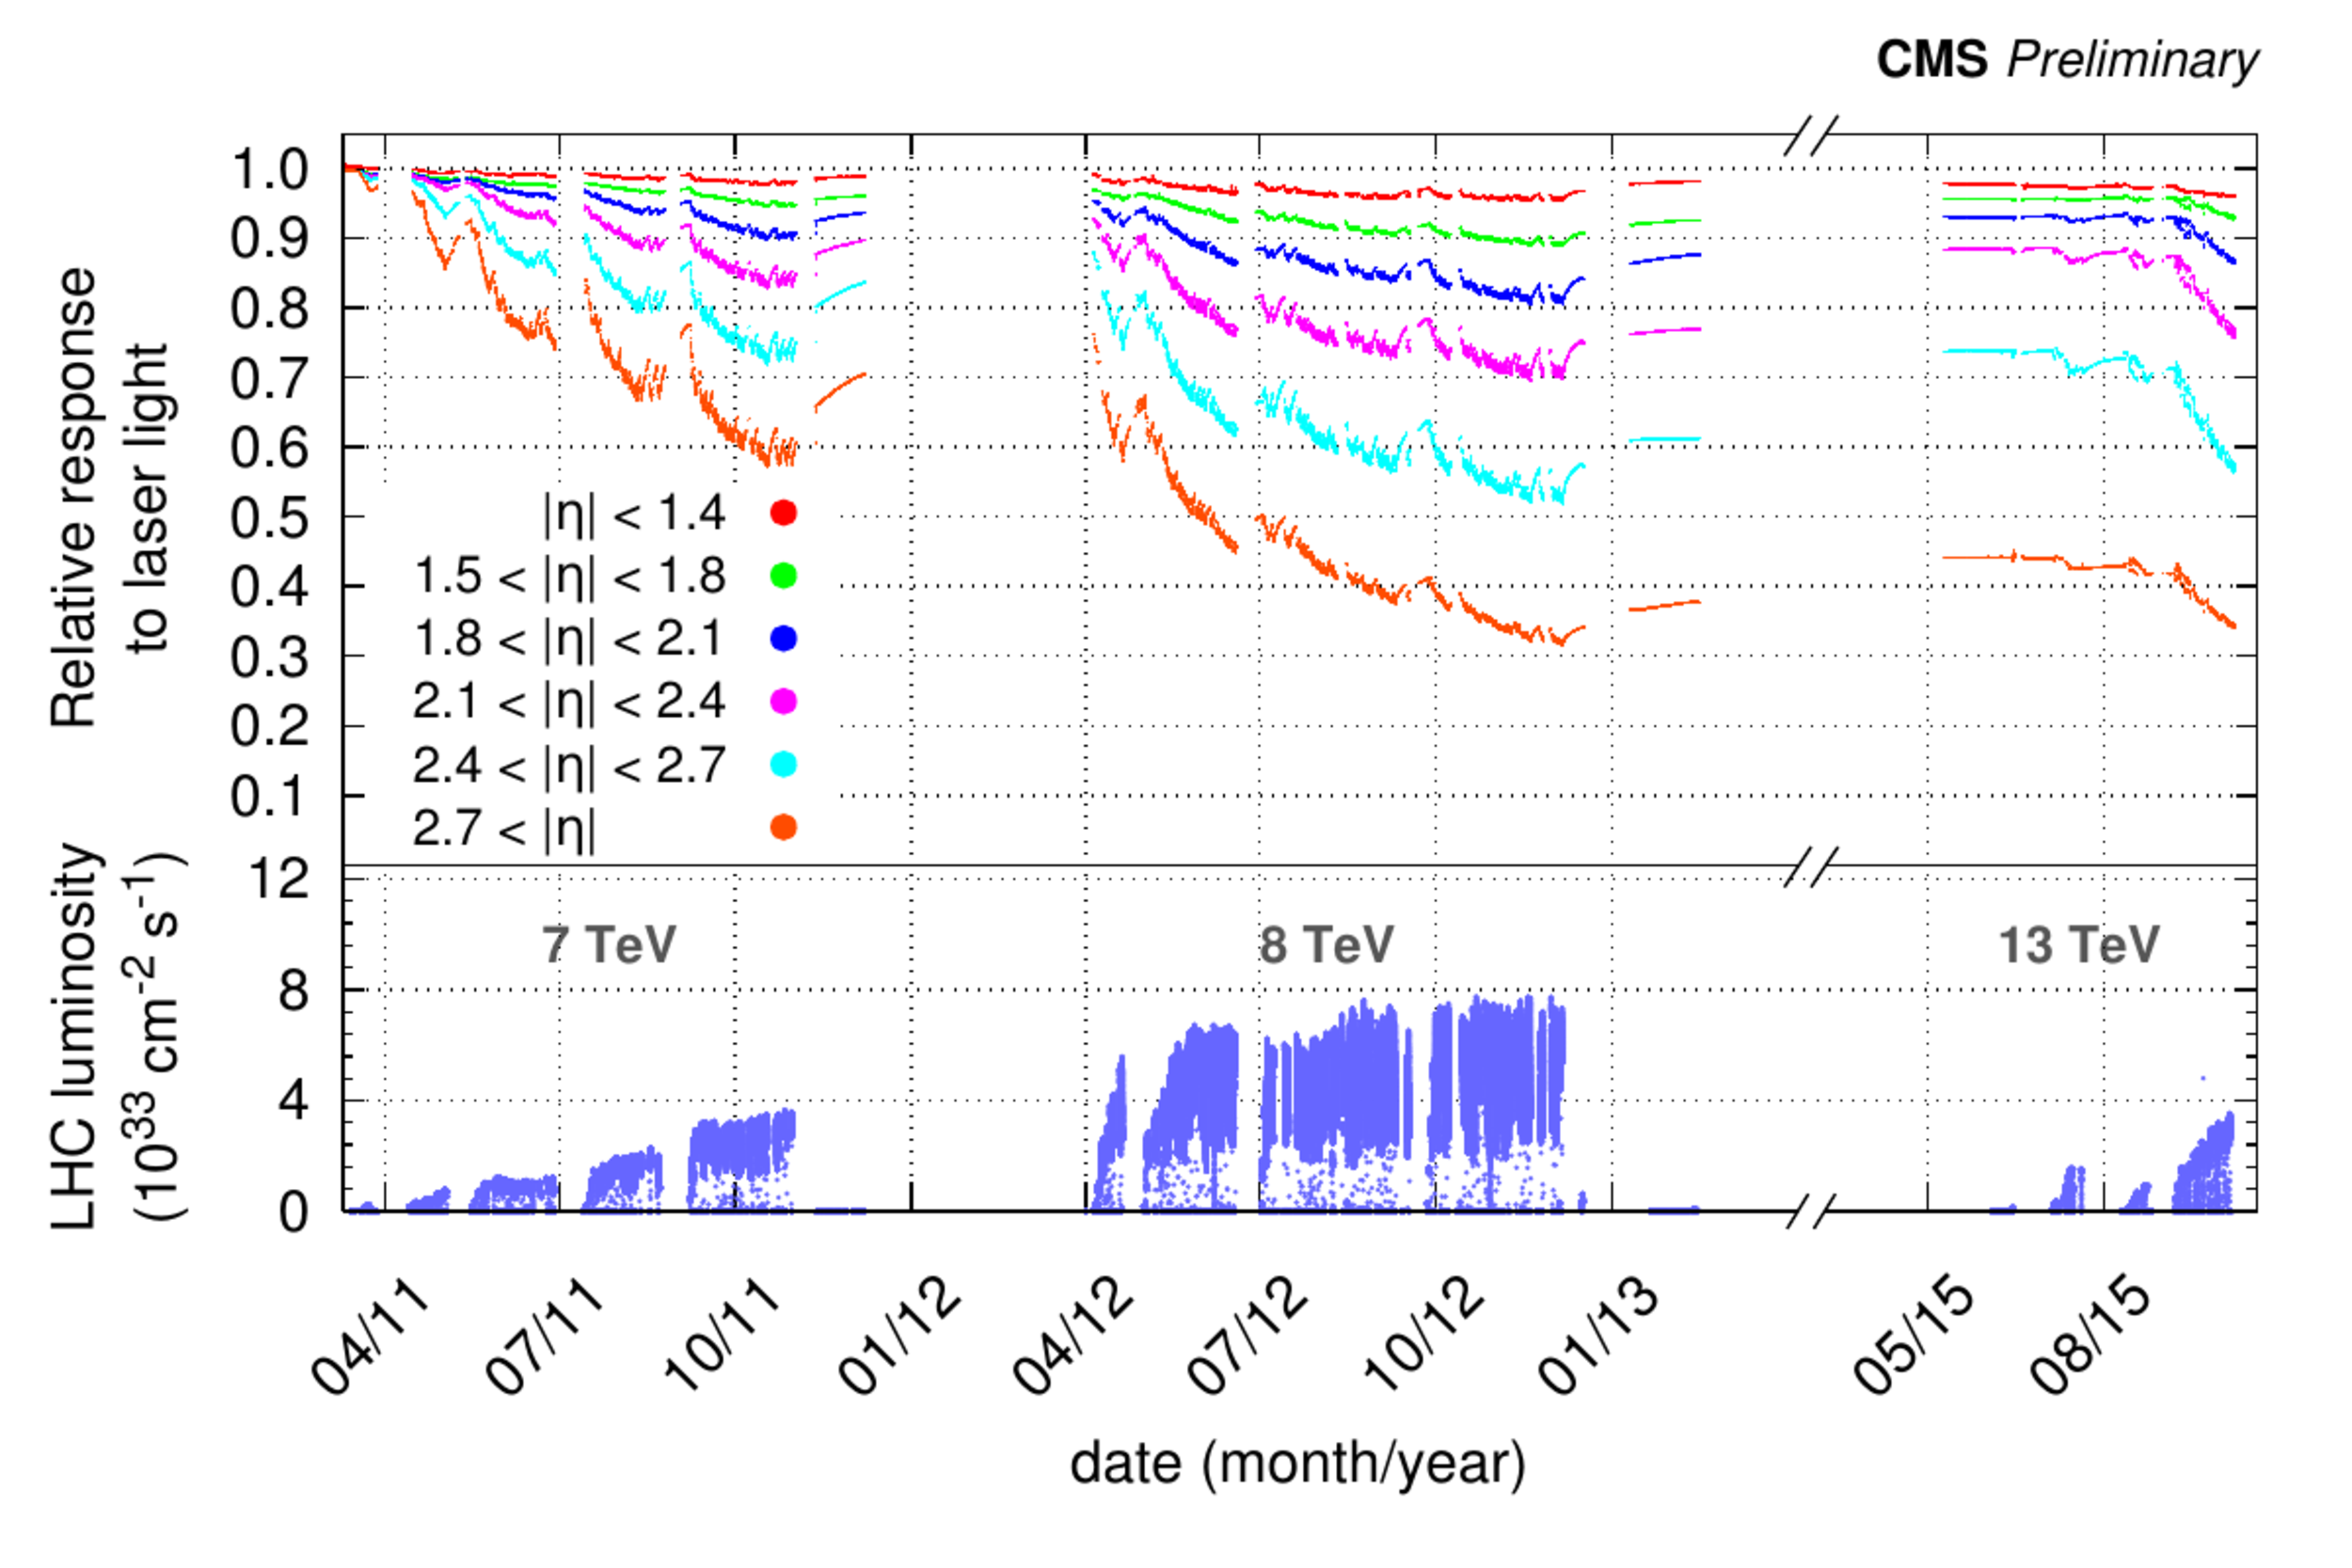
\includegraphics[width=0.8\textwidth]{figures/transparency}\hfil
\caption{History of channel response changes as measured by the light monitoring system.}
\label{fig:fig_laser}
\end{figure*}

In Figure \ref{fig:laser_eop}, it can be seen how the laser corrections impact the stability of the ECAL energy measurement. 
In this plot, the ratio between the energy of an isolated electron as measured by the ECAL (E) and by the CMS Tracker (p) is shown as a function of time. 
Due to the response changes in the crystals and photon detectors, the ratio decreases when left uncorrected. 
After the laser correction is applied, ECAL achieves a stable energy measurement in time.  

\begin{figure*}[tbh]
\centering 
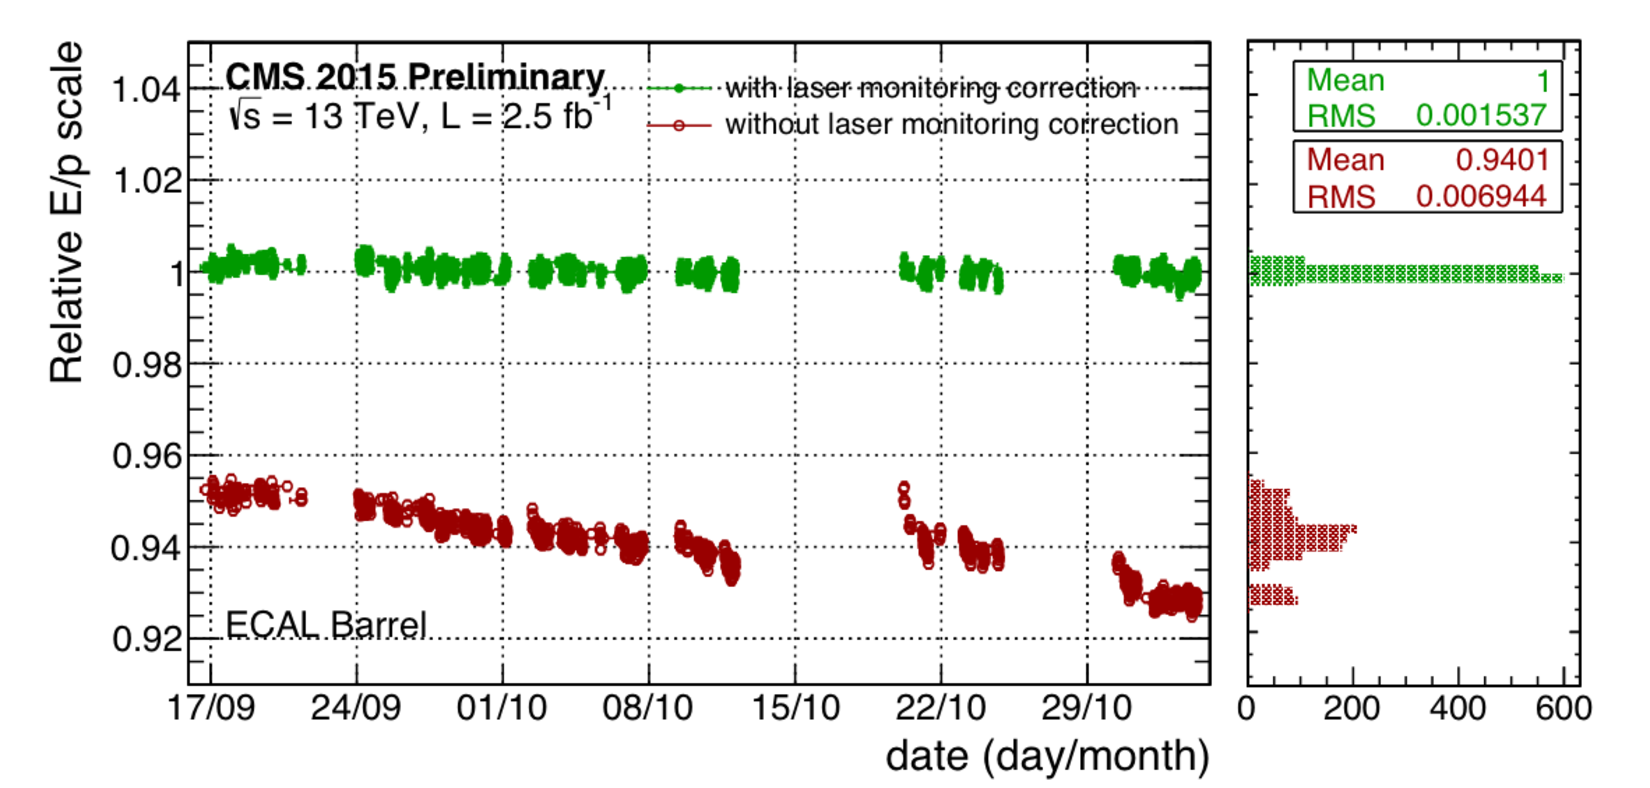
\includegraphics[width=0.8\textwidth]{figures/laser_eop}\hfil
\caption{Stability of electron energy measurement with and without applying laser monitoring corrections.}
\label{fig:laser_eop}
\end{figure*}

\subsection{Intercalibration}

A relative calibration procedure in all ECAL channels is performed to ensure uniformity across the detector. Different and independent methods are used to calculate intercalibration constants (ICs), which are then combined to achieve the desired precision of $<0.5\%$. The final 2015 version of the ICs have been calculated with the full $2.6$ fb$^{-1}$ dataset recorded by CMS with B=3.8 T. The following methods are the same as in Run I \cite{calibration}.

\begin{description}

\item [$\phi$-Symmetry] The $\phi$-symmetry method is based on the expected uniformity of the energy flux along $\phi$ rings (region with fixed $\eta$). The ICs are calculated to correct non-uniformities in this flux. This method was used in 2015 to translate the latest ICs, calculated with the full 2012 dataset, to the 2015 detector conditions. This was done by scaling the 2012 ICs by the ratio between 2015 and 2012 $\phi$-symmetry ICs.

\item [$\pi^{0}/\eta$] The $\pi^0/\eta$ method consists of measuring the invariant mass of these resonances' decays to two photons and maximizing their resolutions by varying the ICs iteratively. This method does not utilize the absolute value of the  $\pi^0$ and $\eta$ resonances not to interfere with the absolute scale calibration. 

\item [E/p] The $E/p$ method employs the same logic as the light monitoring validation method, comparing isolated electron energy and momentum. An iterative method is used to minimize the spread of the $E/p$ distribution.

\end{description}

The combined intercalibration was obtained from the mean of the individual ICs at a fixed value of $\eta$, weighted by their respective precisions. The residual miscalibration of an intercalibration method, which is related to the final method precision, is calculated as the spread of the difference between the method's ICs and the other methods' ICs at a fixed value of $\eta$. 
This residual miscalibration can be seen in Figure \ref{fig:ecal_miscalib}  (left) for the ECAL barrel, where it is shown that 
The combination of ICs achieves the desired goal of less than $0.5\%$ precision for the central barrel region. 
The overall impact of applying the intercalibration constants and the response monitoring corrections can be seen in Figure \ref{fig:ecal_miscalib} (right), in $Z\rightarrow ee$ events.

\begin{figure*}[tbh]
\centering 
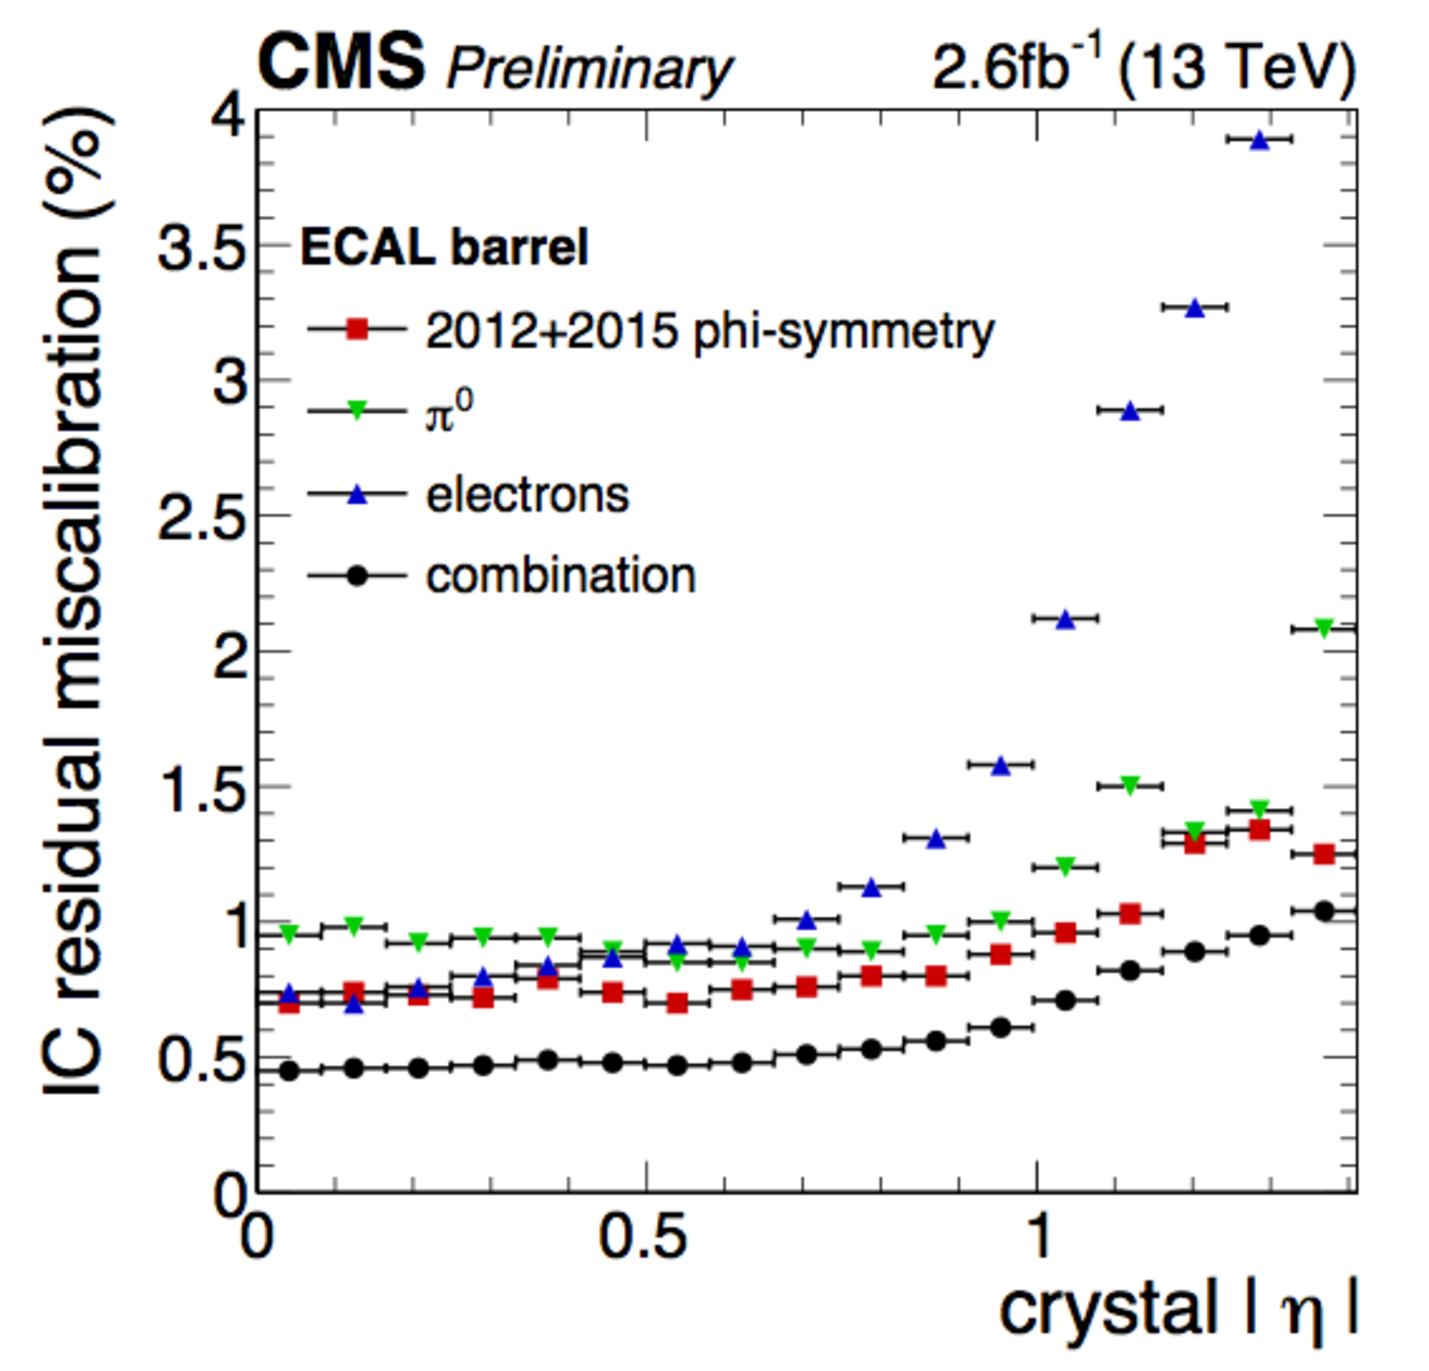
\includegraphics[width=0.45\textwidth]{figures/ecal_miscalib}\hfil
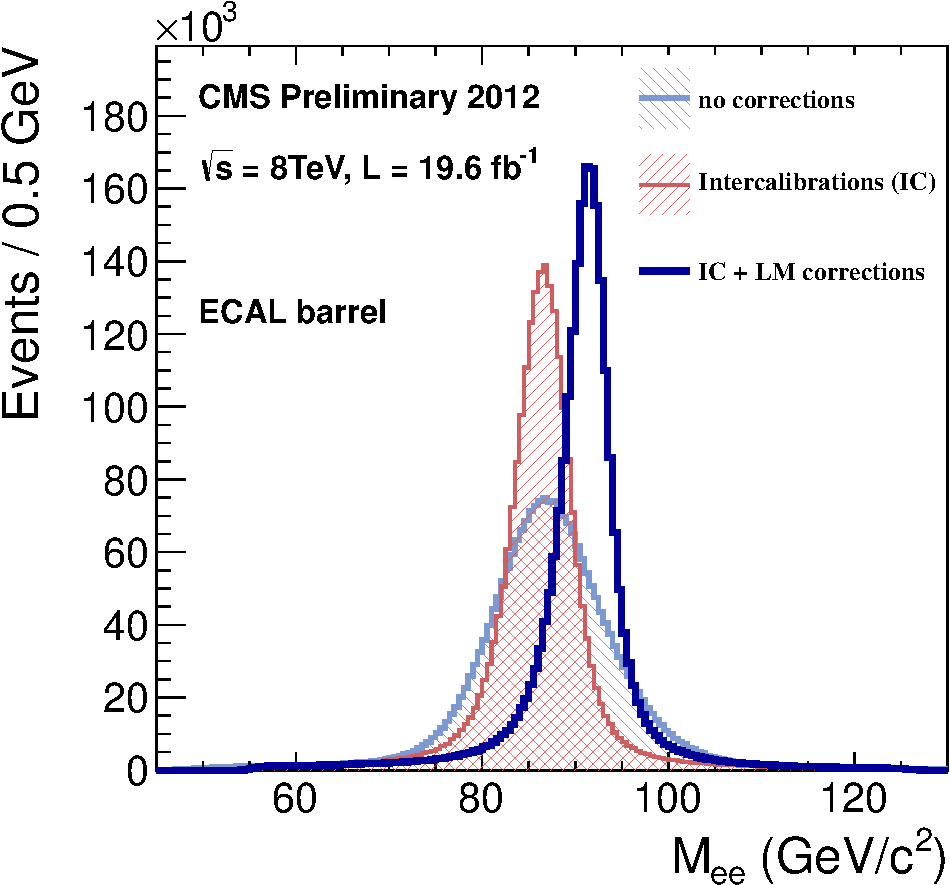
\includegraphics[width=0.45\textwidth]{figures/ecal_ic_lm}\hfil
\caption{Residual mis-intercalibration with the different ECAL intercalibration methods and their combination.}
\label{fig:ecal_miscalib}
\end{figure*}


\subsection{Absolute Calibration}

$Z\rightarrow ee$ events are used both to set the $\eta$ scale and the absolute calibration \cite{calibration}. The first is developed to ensure that  different $\eta$ regions have the same relative response, while the second (done separately for barrel and endcaps) sets the absolute energy scale.

A dedicated calibration was performed with 0 T data to account for differences in shower shapes in the absence of magnetic field. For example, in 0 T there is no bremsstrahlung radiation outside the main electron cluster deposit, improving the reconstructed energy resolution.

In addition, the calibration was validated with high energy photons and electrons.
%being used in analyses searching for high mass resonances decaying in those particles.
The validation was performed by comparing data and Monte Carlo simulations for high energy electrons from $Z\rightarrow ee$. The calibration was found to be stable to $0.5\%$ ($0.7\%$) for electrons up to $p_{T}=150$ GeV in the barrel (endcap). Possible saturation effects were corrected for with a multivariate technique, but those effects were found to be $<2\%$ for photons arriving from resonance masses less than $1.4$ TeV.

\subsection{High Level Calibrations}

The amount of material in front of ECAL, up to $2X_0$ in the barrel outer regions as seen in Figure \ref{fig:ecal_cluster} (left), produces a high rate of bremsstrahlung radiation from electrons and a high probability of photon conversions. To mitigate this effect, a clustering algorithm is used to recombine energy deposits that come from those processes. The cluster energy is corrected via a multivariate technique, separately for photons \cite{photons} and electrons \cite{electrons}. It also aims to correct other effects, such as in time pile up. The effect of these high level cluster corrections on the resolution of the $Z\rightarrow ee$ peak can be seen in Figure \ref{fig:ecal_cluster} (right).

\begin{figure*}[tbh]
\centering 
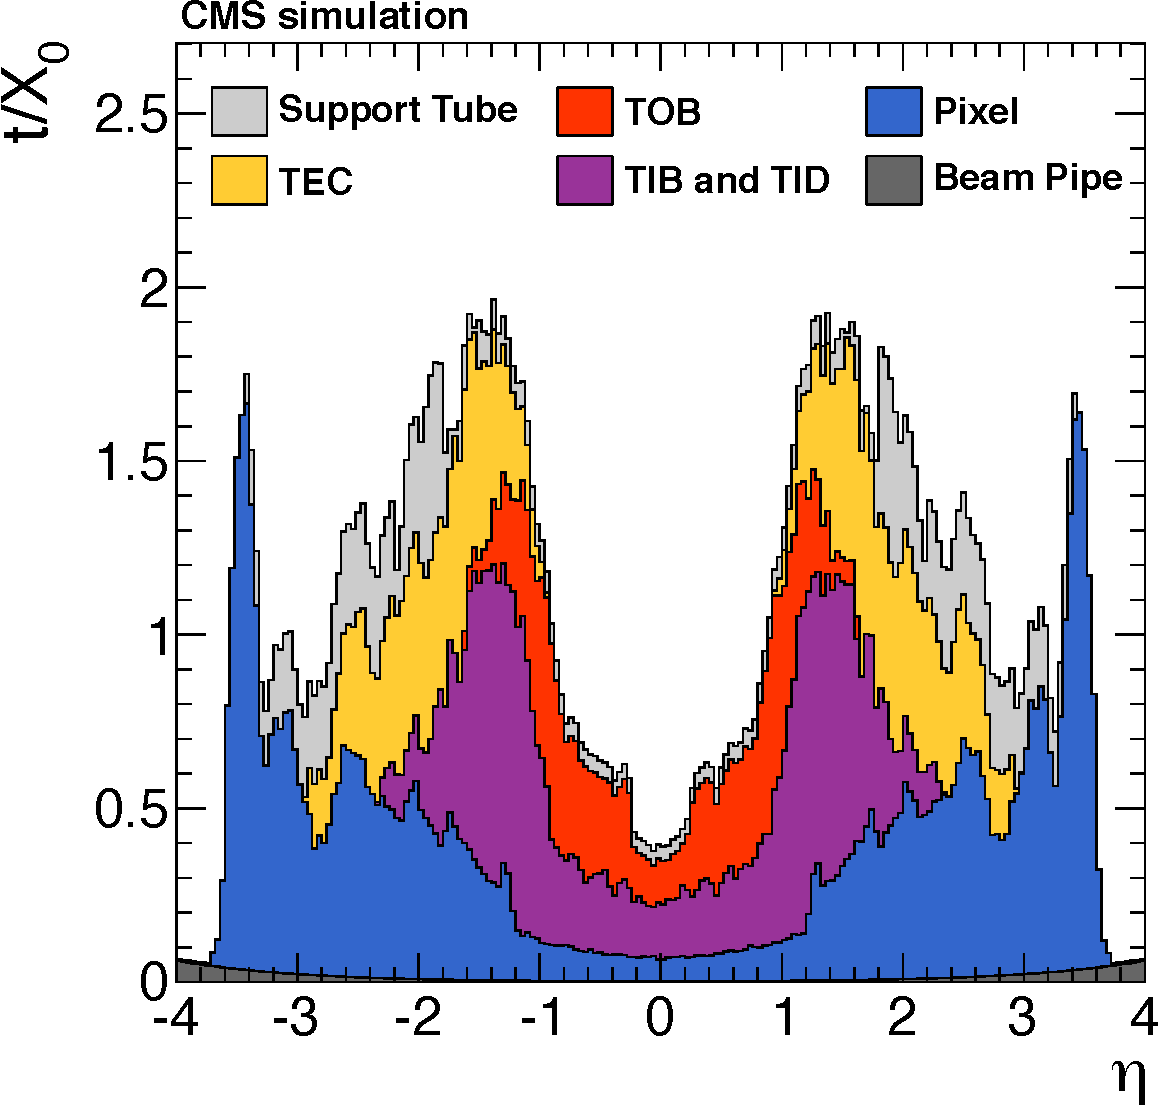
\includegraphics[width=0.45\textwidth]{figures/cms_material}\hfil
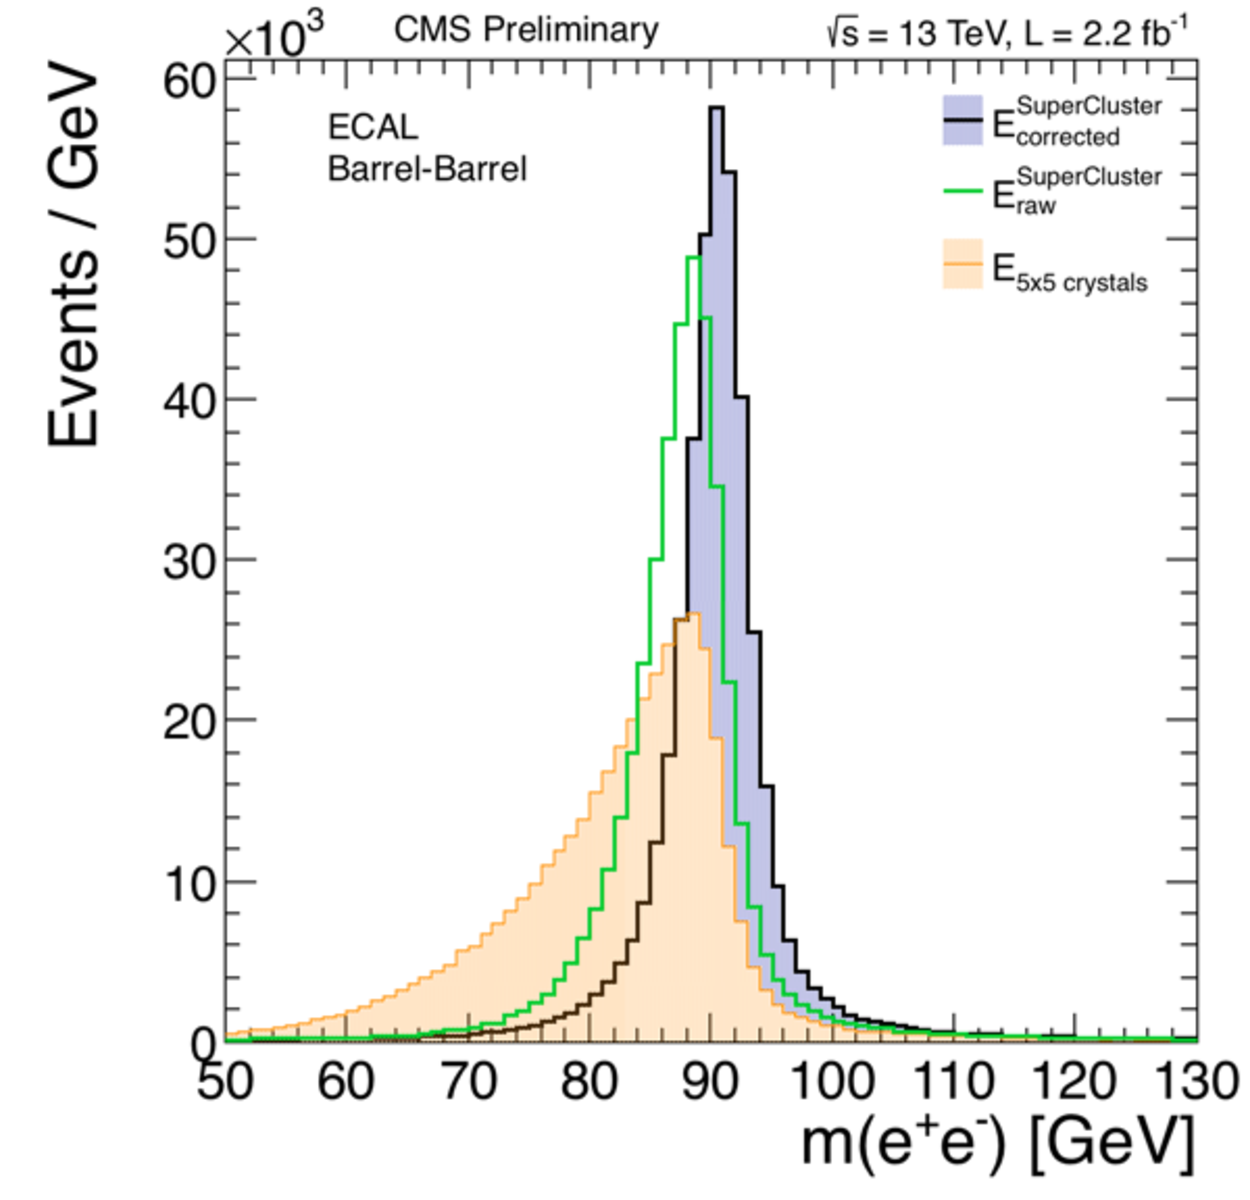
\includegraphics[width=0.45\textwidth]{figures/ecal_clustercorr}\hfil
\caption{Material budget between the ECAL and the collision point on CMS (left). Effect of high level cluster corrections on the resolution of the $Z\rightarrow ee$ peak.}
\label{fig:ecal_cluster}
\end{figure*}


\section{ECAL Energy Resolution}

\subsection{Energy Resolution of a Calorimeter}

The intrinsic energy resolution of an electromagnetic calorimeter can be parametrized in terms of three sources, as in the following equation:

\begin{equation}
\frac{\sigma}{E}  = \frac{A}{E} \oplus \frac{B}{\sqrt{E}} \oplus C,
\end{equation}

where the first term on the right-side of the equation is called the noise term, the second is called the stochastic term and the third, the constant term. 
A brief explanation of the physical nature of these uncertainties follows:

\begin{description}
\item [Noise term] The noise term is the contribution to the energy resolution from the electronic noise in the readout chain. In the case of ECAL, this noise comes from the VFE and FE part of the detector, specially in the light detection phase by the photo-detectors and on the amplification and sampling phase by the MGPA. 
\item [Stochastic term] This contribution to the resolution comes from the physical development of the shower shape inside the detector. For homogeneous detectors, such as ECAL, this term is usually small, since the full shower development is contained within the active medium. 
\item [Constant term] Differently from the other two terms, this one is independent of the energy of the incoming particle in the detector. This uncertainty is related to geometrical and static features of the detector, such as non-uniformities and random instabilities in response that are independent on energy. On ECAL, this contribution is largely mitigated by the intercalibration and laser monitoring calibration.
\end{description}

During the ECAL test-beam commissioning period, these terms were measured directly as: A = 128 MeV, B = 2.8 $\sqrt{\text{GeV}}$ and C = 0.3 \%.

\subsection{ECAL Energy Resolution with Run II data}

The ECAL energy resolution is measured using $Z\rightarrow ee$ events, from an unbinned fit with a Breit-Wigner function convoluted with a Gaussian as signal model. Degradation effects come from the amount of material in front of ECAL and cracks between modules. The resolution, as a function of $\eta$, for low bremsstrahlung electrons in the barrel can be seen in Figure \ref{fig:ecal_res}.

\begin{figure*}[tbh]
\centering 
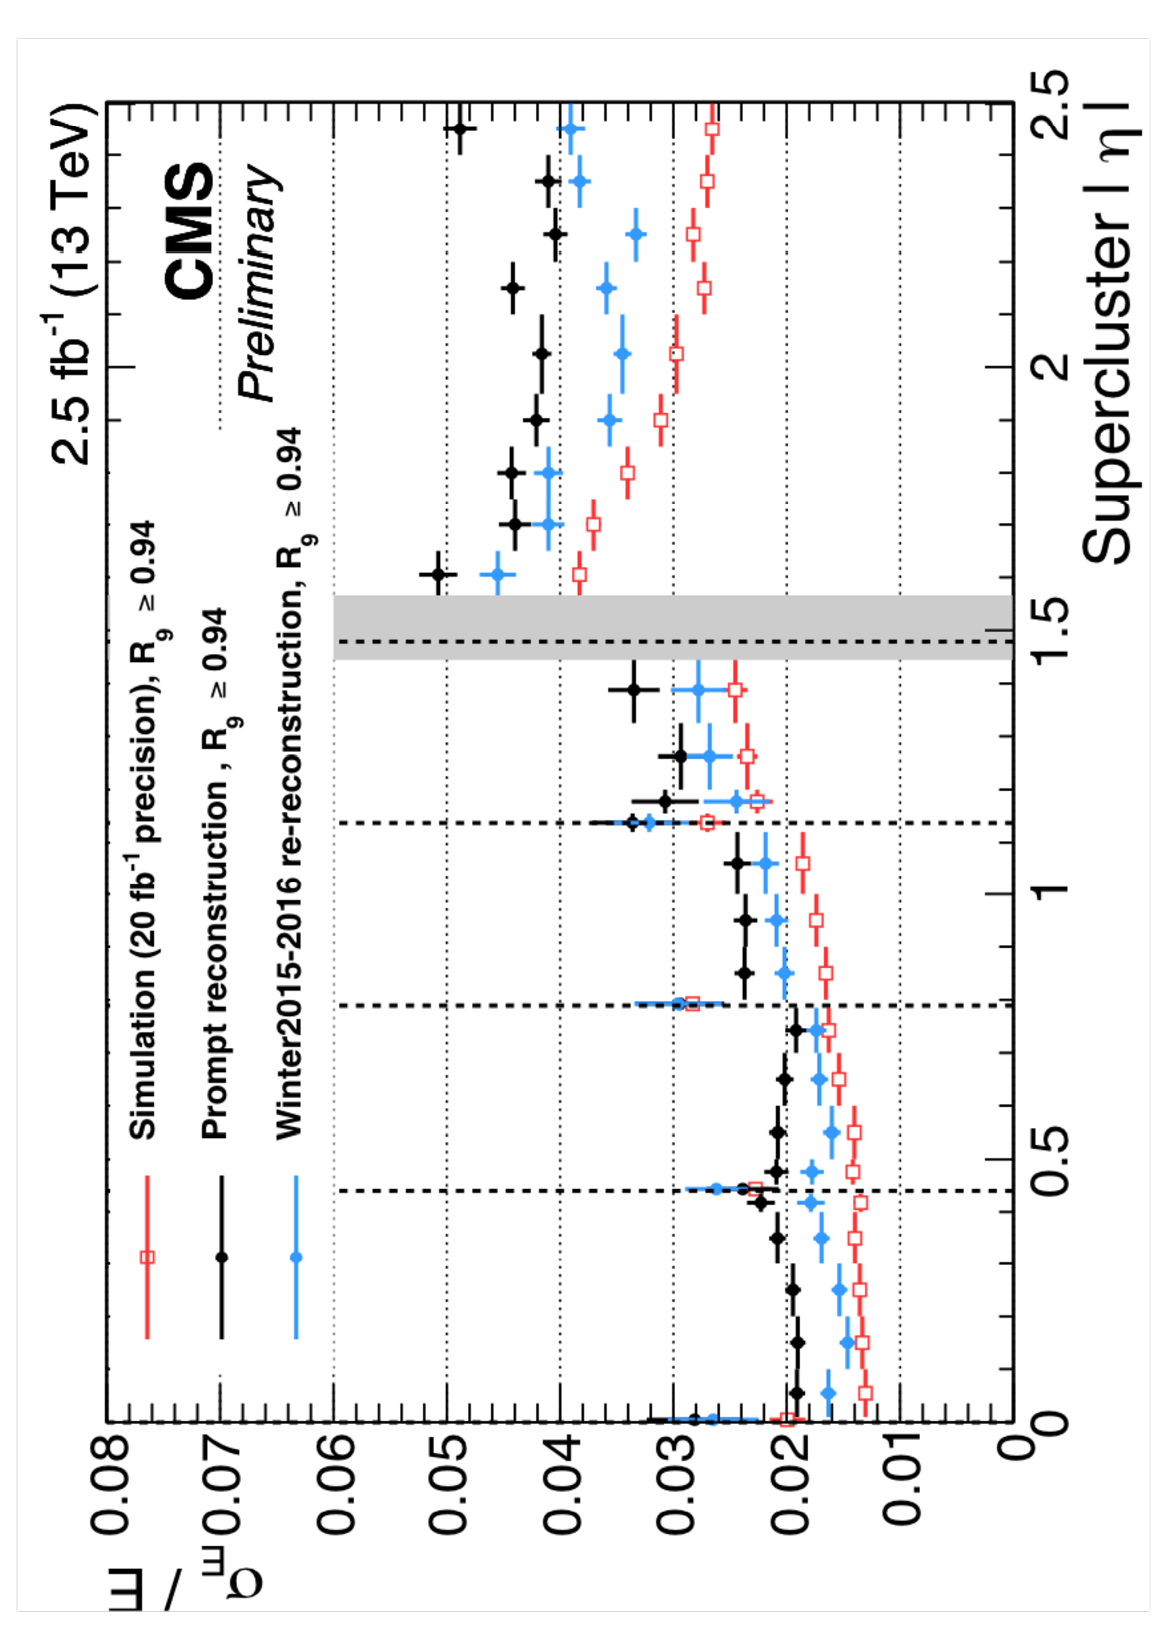
\includegraphics[height=0.45\textwidth, angle=270]{figures/ecal_res_HighR9.pdf}\hfil
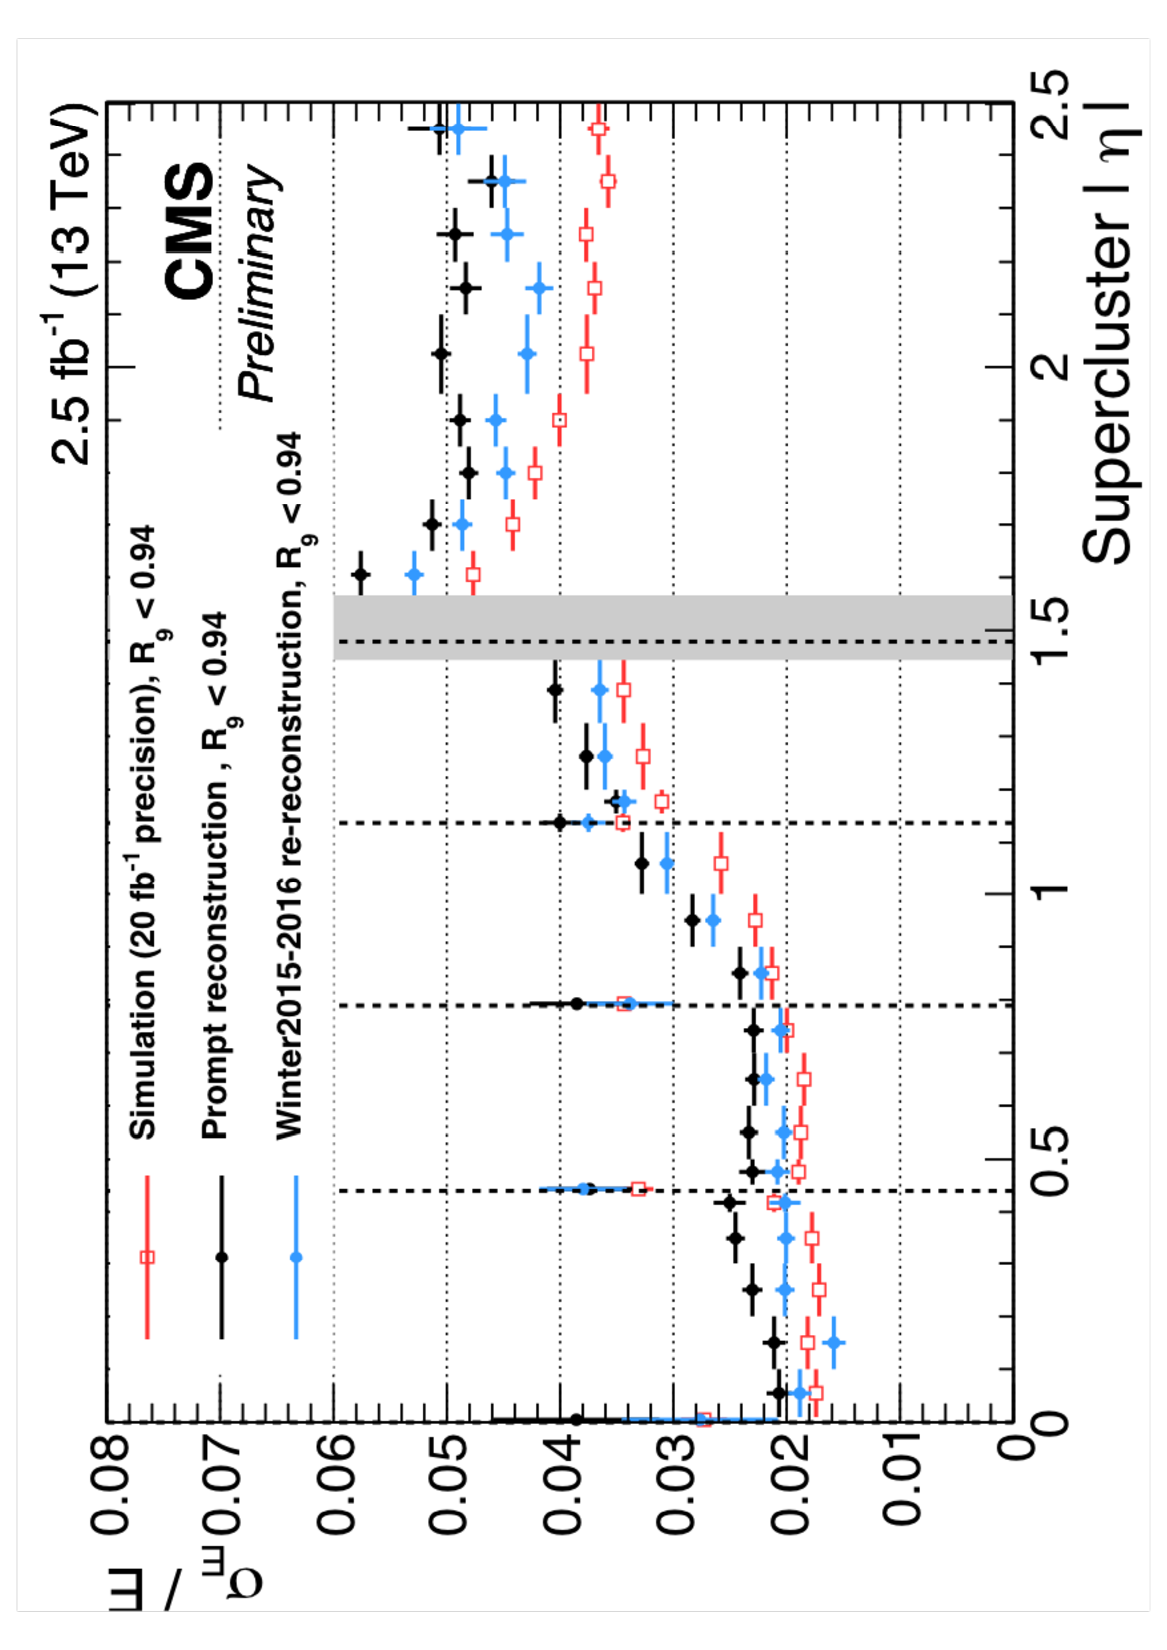
\includegraphics[height=0.45\textwidth, angle=270]{figures/ecal_res_LowR9.pdf}\hfil
\caption{Energy resolution for low (left) and high (right) brehmsstrahlung $Z\rightarrow ee$ electrons as a function of $\eta$.}
\label{fig:ecal_res}
\end{figure*}


The energy resolution achieved with reprocessed data, which includes the latest intercalibration and calibration constants derived with 2015 data, achieves a resolution that is less than 2$\%$ for $Z\rightarrow ee$ low bremsstrahlung electrons in the central barrel region.
%The energy resolution achieved using the latest 2015 calibration constants is less than $2\%$ for low bremsstrahlung electrons in the barrel.
The reprocessed data is especially better performing in the endcaps, when comparing to processed data with 2012 values for intercalibration and calibration. When ported to physics analysis, this energy resolution implies, for example, in a $\sigma_{eff}/M_h \approx 1.5\%$ (from simulation) in the $H\rightarrow\gamma\gamma$ analysis, where $\sigma_{eff}$ is the smallest interval in $M(\gamma\gamma)$ with $68.5\%$ coverage \cite{hgg}.


\section{The CMS ECAL Barrel Upgrade}
\subsection{The High Luminosity LHC}

The performance of the Large Hadron Collider, and the physics program carried by ALTAS and CMS, has started remarkably. With the discovery of the Higgs boson in 2012, and the expected 40 fb$^{-1}$ to be delivered in 2016 with record high instantaneous luminosity, the program has exceeded experimental expectations. The current LHC setup, with bunch spacing of 25 ns and peak instantaneous luminosity of the order of $10^{34}$ cm$^{-2}$s$^{-1}$, is expected to deliver around 300 fb$^{-1}$ until the end of 2022, when the Long Shutdown 3 (LS3) is planned to start.

During LS3, which is planned to last until 2025, the LHC is expected to replace the quadrupoles that focus the beam for ATLAS and CMS. Additionally, upgrades will be performed to optimize the bunch overlap at the interaction region. These improvements are expected to allow the LHC peak luminosity to reach $2\times10^{35}$ cm$^{-2}$s$^{-1}$ (High Luminosity LHC, HL-LHC). During the following 10 years, 250 fb$^{-1}$/year are expected to be delivered. This full dataset of around 2500 fb$^{-1}$ will open a brand new physics program at the LHC, involving precise measurements of the Higgs properties and rarer standard model phenomena, such as the standard model Higgs pair production. 

The new LHC configuration will also bring new experimental challenges. With the increased peak luminosity, a higher dose of radiation will be reaching the inner detectors of ATLAS and CMS, causing unrecoverable losses of efficiency in tracking reconstruction and calorimetry, for example. It will also challenge the online performance of the detectors, forcing the trigger systems to cope with higher event rates. To recover their performances to comparable or higher levels of the previous data taking periods, ATLAS and CMS have planned hardware upgrades to be deployed during LS3.


\subsection{ECAL Electronics Upgrade}

As mentioned in the previous section, the impact of incoming radiation on ECAL is to form color centers on the crystals that damage its transparency. 
With the incoming dose of radiation at the HL-LHC, the endcap crystals are expected to completely lose their transparencies. 
This prompted the CMS community to entirely replace the ECAL endcaps for its HL-LHC upgrade. 
The new ECAL endcap will be based on silicon technology, as a sampling calorimeter (HGCal). 

On the ECAL barrel, the crystals are expected to robustly cope with the incoming dose of radiation, and will therefore be kept in the detector. 
However, the new levels of radiation will also represent a challenge to the in-detector electronics. 
For example, the dark current on the APDs (the electric current flowing through the photo-detector even in the absence of signal, created by random processes) is expected to increase, given the higher ionizing radiation dosage hitting the detector. 
This dark current is a large contributor to the noise term in the energy resolution formula, specially to homogeneous calorimeters, and upgrades must be devised to keep it under control. 

\subsubsection{VFE Upgrade}

For the HL-LHC upgrade, two ways to mitigate the increased detector noise have been investigated: replacing the VFE and cooling the ECAL crystals and APDs from 18$^{o}$C to 8$^{o}$C. 
The APDs cooling works reducing the dark current expected at high integrated luminosities scenario. 
The downside of this upgrade is the decreased light yields from scintillation from the lead tungstate crystals. 
The VFE upgrade intends to reduce the electronics noise by reducing the shaping time attached to the amplifying process, currently is 40 ns. 
This reduction limits the impact of electronics noise in the amplitude reconstruction, while also allowing for a more precise time resolution from ECAL. 
These improvements can be seen in Figure \ref{fig:ecal_noise_intlumi} (left). 
Figure \ref{fig:ecal_noise_intlumi} (left) also shows that, in the scenario with no HL-LHC upgrades, the noise present on the ECAL barrel would reach levels almost 10 times higher than the current value (1.5 ADC counts). 
The upgrade reduces the noise at 3000 fb$^{-1}$ by a factor of almost 2. 

\begin{figure*}[tbh]
\centering 
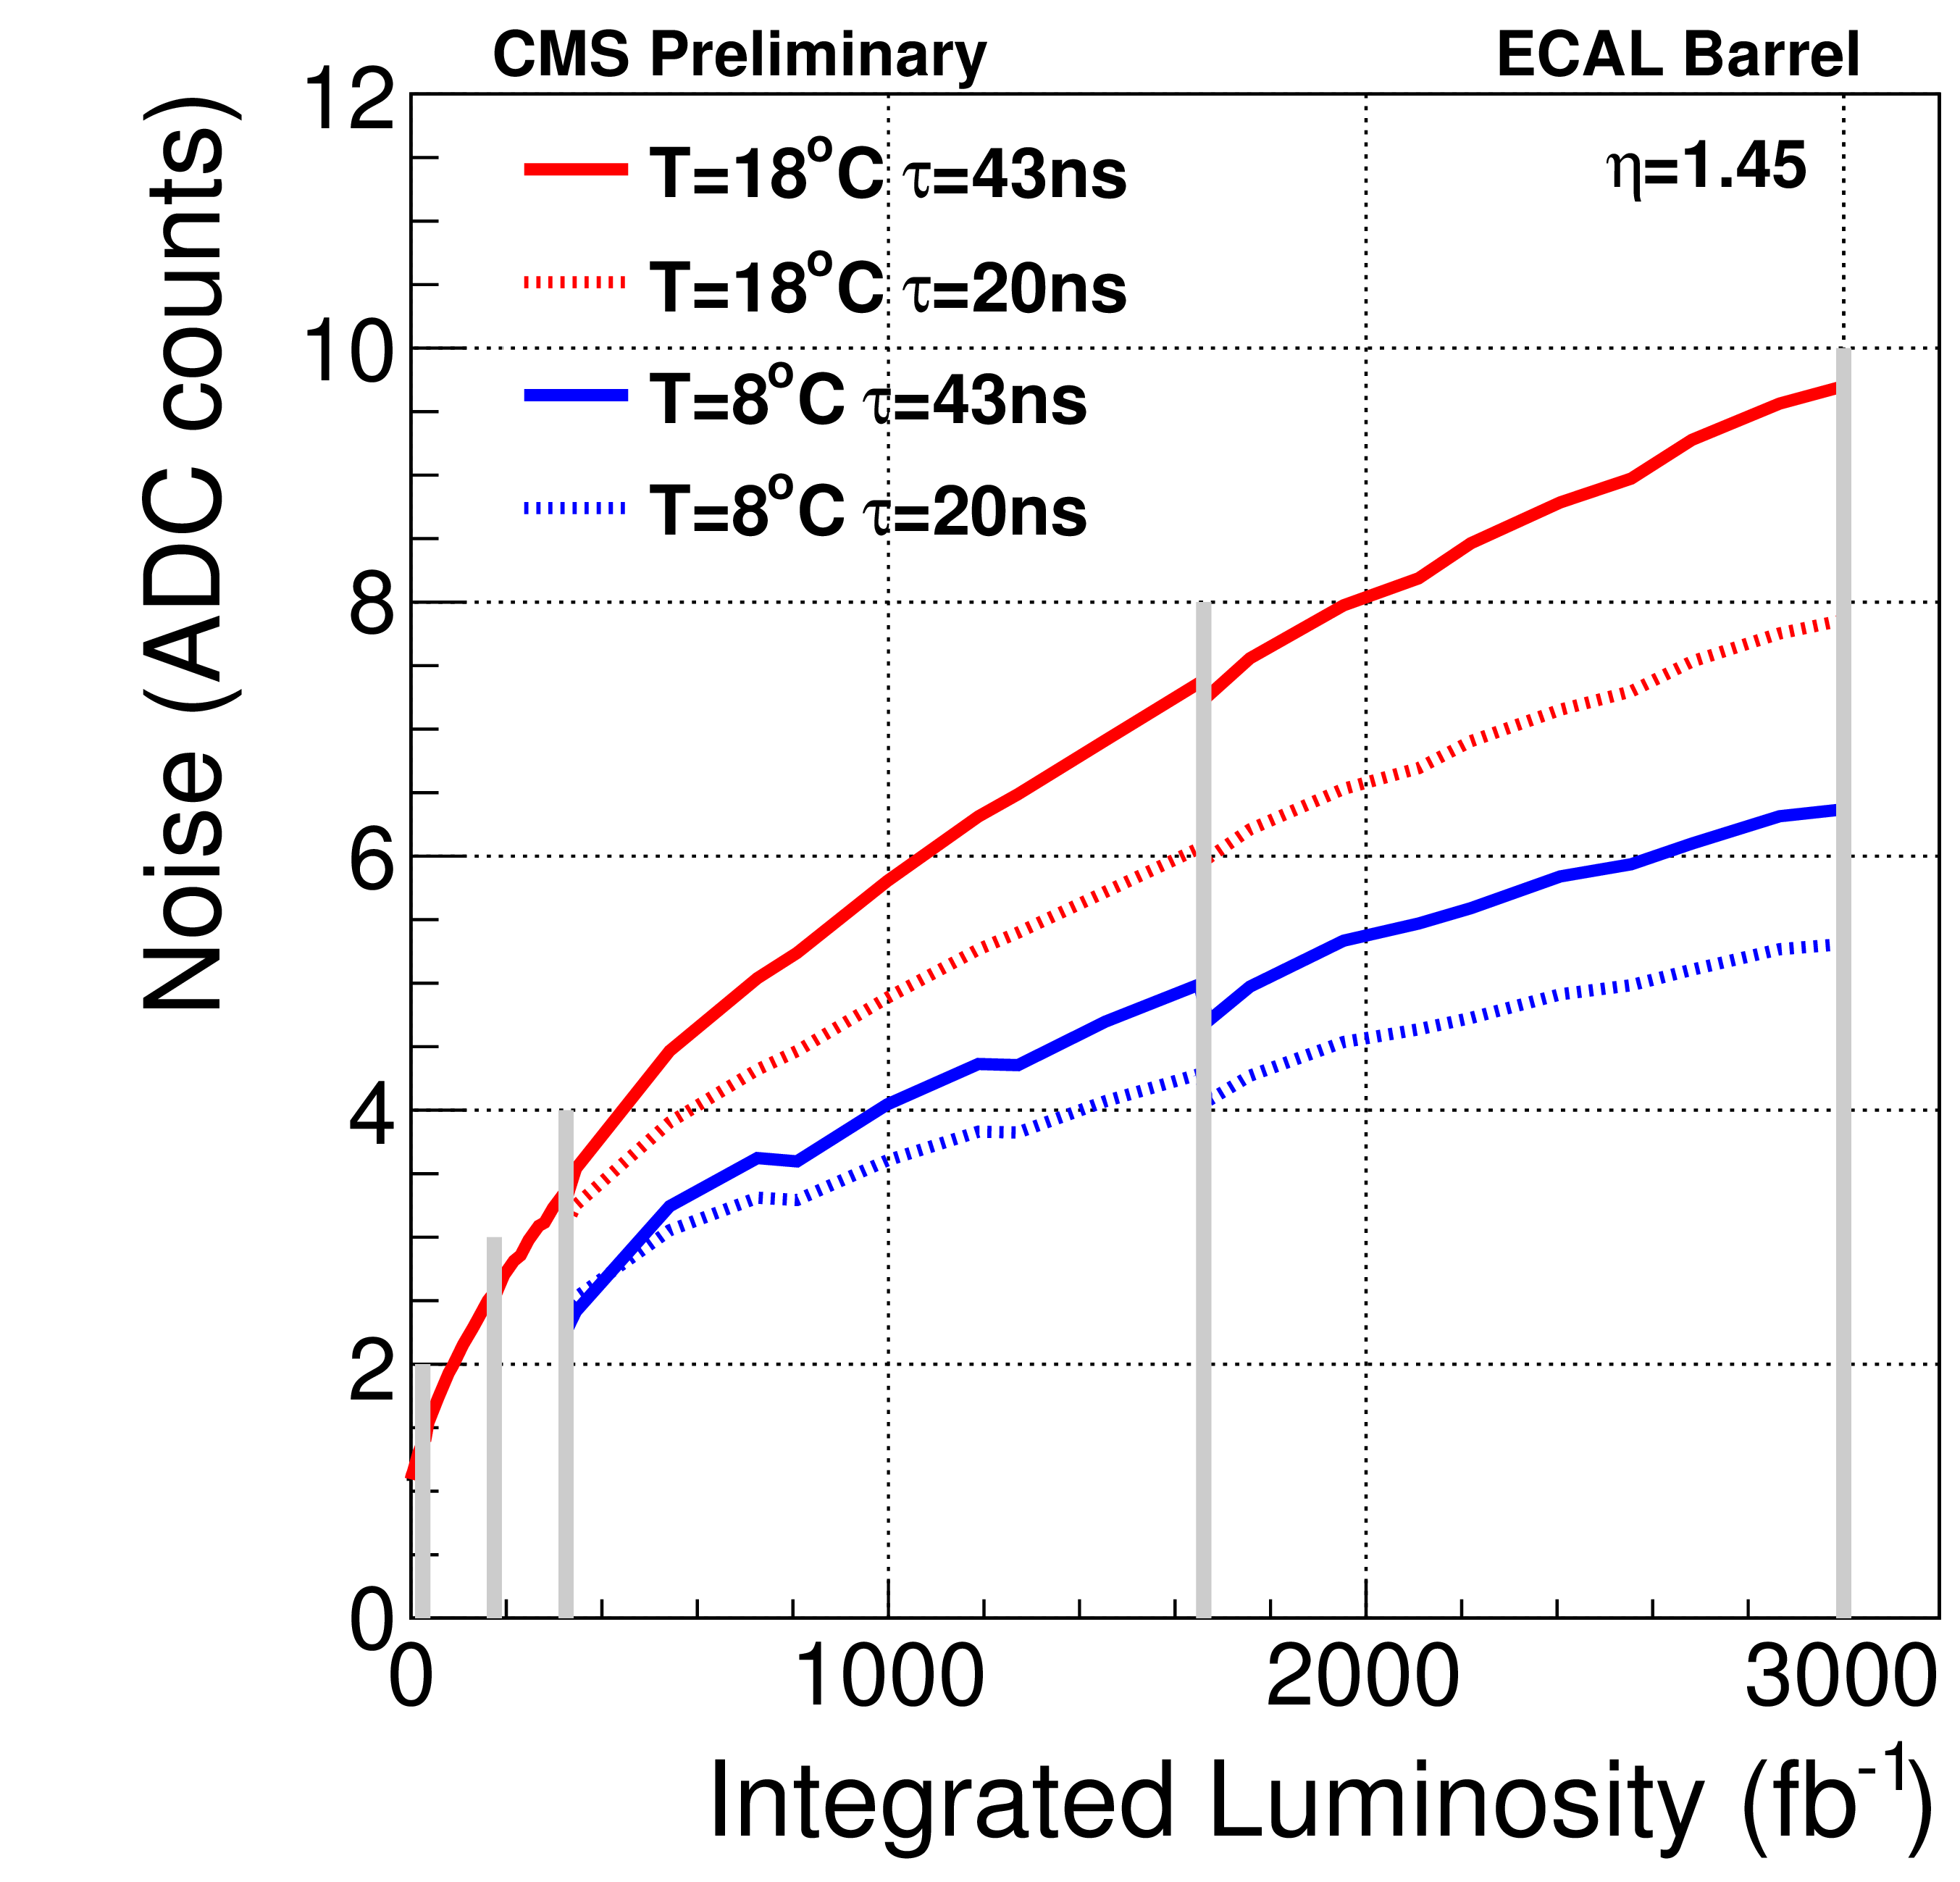
\includegraphics[width=0.45\textwidth]{figures/ecal_noise_intlumi}\hfil
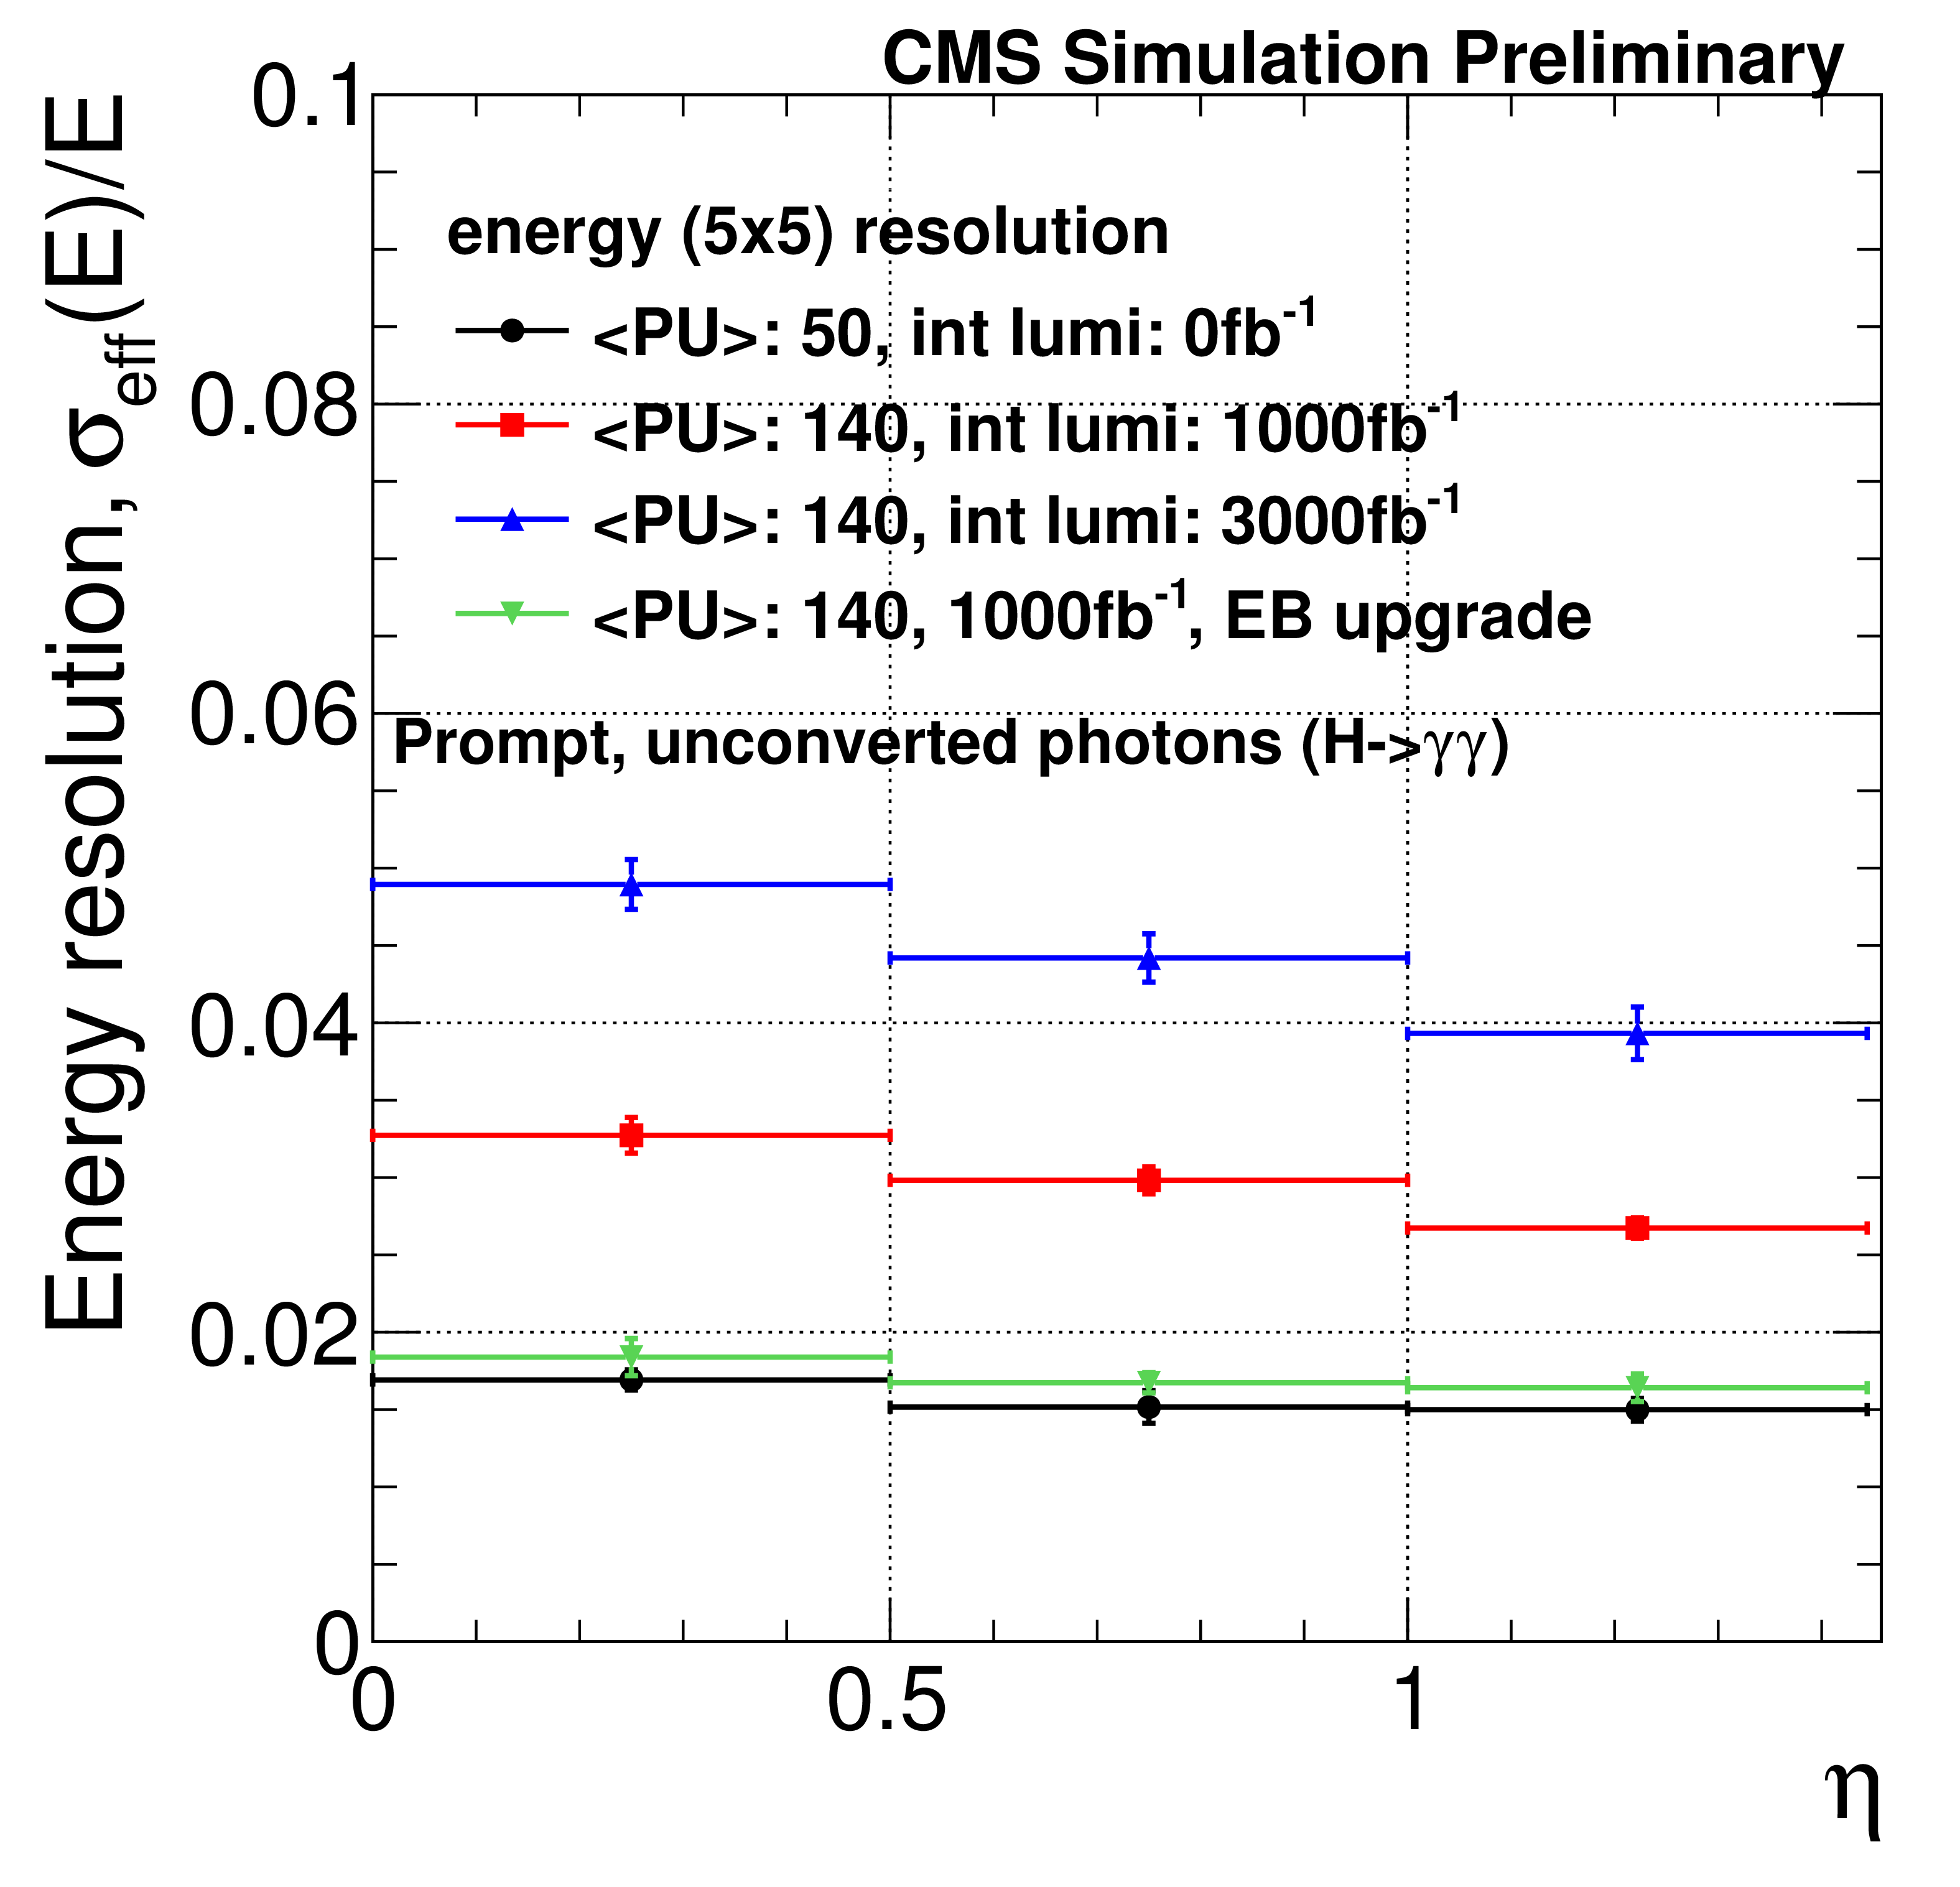
\includegraphics[width=0.45\textwidth]{figures/ecal_upgrade_performance}\hfil
\caption{Noise levels on the upgraded ECAL barrel assuming different upgrade scenarios.}
\label{fig:ecal_noise_intlumi}
\end{figure*}

The noise reduction is translated into physics performance, for example, in $H\rightarrow\gamma\gamma$ searches, as seen in Figure \ref{fig:ecal_noise_intlumi} (right). 
Figure \ref{fig:ecal_noise_intlumi} (right) shows the energy resolution of good quality  $H\rightarrow\gamma\gamma$ photons under different integrated luminosity scenarios, with and without the ECAL barrel upgrade. 

\subsubsection{Trigger Upgrade}

Another important issue arising from the HL-LHC environment is the increase in electronic spikes in the APDs. 
These spikes are created when a high energy hadron hits the APDs directly, without showering in the ECAL crystals. 
This creates an energy discharge in the APD that can fake a signal from a regular particle shower. 
Spikes are problematic when they happen with high frequency because they enhance L1 trigger rates. 
These trigger must then have high energy thresholds in order for the rates to be acceptable by the CMS L1 trigger. 

Another way currently implemented to suppress spikes at trigger level is through coarse geometric variables. 
These variables are computed at the trigger primitive generation step, at the front-end electronics. 
Due to computational limits of the FE boards, these variables use limited information about the crystal array. 
This can be changed if the TP generation happened at the off-detector electronics instead. 
However, this would mean transmitting the full crystal information of the whole ECAL to the off-detector electronics at collision rate (40 MHz). 
By the time of the ECAL commissioning period, the data links could not cope with such requirements, and so the trigger tower based TP generation was implemented. 

One of the foreseen ECAL barrel upgrades is aimed at mitigating those constraints by moving the TP generation step to the off-detector electronics. 
New data links will be used to transmit all crystal data directly from the VFE, instead of being stored waiting for an L1A. 
With extra computing power based on modern FPGAs, new strategies can be investigated to reduce the impact of spikes at L1 trigger level. 
One of these strategies is based on analyzing the signal pulse shape coming from the crystals. 
Given the smaller shaping time from the upgraded VFE, differences in pulse shapes from regular energy showers and spikes can become visible for ECAL.

\chapter{Exotic Higgs Decays in $\gamma+$MET Final States}

Lorem ipsum dolor sit amet, consectetur adipiscing elit, sed do eiusmod tempor incididunt ut labore et dolore magna aliqua. Ut enim ad minim veniam, quis nostrud exercitation ullamco laboris nisi ut aliquip ex ea commodo consequat. Duis aute irure dolor in reprehenderit in voluptate velit esse cillum dolore eu fugiat nulla pariatur. Excepteur sint occaecat cupidatat non proident, sunt in culpa qui officia deserunt mollit anim id est laborum.
\section{Run-1 CMS $H\rightarrow\gamma$+MET Analysis}
\section{$H\rightarrow\gamma\gamma$+MET Projection Studies}
Einstein's paper: \cite{Einstein}

\chapter{HH searches with photons and b-jets at CMS Run 2}
\graphicspath{{hh/figures/}{hh/}}
\section{Introduction}
This chapter describes the inclusive search for the double Higgs production process in the decay
mode $\HH \to \bbgg$ at $\sqrt{s}=13\TeV$, with $36.5$ fb$^{-1}$ from the 2016 data taking period. 
This analysis is based on the search at 8\TeV performed in the same final state, recently published by CMS in
Ref.~\cite{HIG-13-032} (the internal CMS documentation of this analysis can be found in Refs.~\cite{AN-13-075,AN-14-118}), and 
on the earlier 13\TeV search using 2015 data \ref{bbgg_2015}.

Many theories beyond the SM (BSM) suggest the existence of new physics potentially manifested in the detection of a pair of Higgs bosons. 
The simplest signal we can look for is in the form of a resonant contribution to the invariant mass of the HH system (resonant search). 
%If the new particles are too heavy to be observed through a direct search, that we will call the resonant serach.
If the BSM new particles are not directly detectable (either too heavy or too light to be in the HH invariant mass spectrum), but still couple to HH, their virtual contribution to the non-resonant HH production can still be measured (as shown, e.g., in Refs.~\cite{Dawson:2015oha,Cao:2013si}). Additionally, the fundamental couplings of the Higgs boson to other SM particles (including itself) can be modified as well in BSM theories (as shown, e.g., in Refs.~\cite{Mangano:2002ea,Grober:2015cwa}). Both of these cases can be studied via the non-resonant HH process.

In order to study the HH production, the Higgs bosons' final states must be carefully chosen. On one hand, the overall cross section of the process must be kept high enough for a good sensitivity. On the other hand, a good selection efficiency, online and offline, is important for a well performing analysis. This is achieved with the $\bbgg$ final state. The $\Hbb$ leg provides a high branching ratio ($57.7\%$), while the $\Hgg$ leg provides an efficient way to correctly identify the interesting events and a high mass resolution. The total branching ratio of the $\HH\to\bbgg$  channel is $0.26\%$.

%If however those are not directly detectable (too heavy ot too light) they may be sensed in the HH production through their virtual contributions (as shown, e.g., in Refs.~\cite{Dawson:2015oha,Heng:2013cya}); also, the fundamental couplings of the model can be modified relative to their SM values (as shown, e.g., in Refs.~\cite{Grober:2010yv,Moretti:2004wa}); in both cases, a nonresonant enhancement of the HH production could be observed.  
%The $\bbgg$ final state has the advantages of a large branching fraction of the $\Hbb$ decay and a good mass resolution of
%the $\Hgg$ decay. The total branching fraction of this channel,
%$\mathcal{B}(\HH\to\bbgg)$, is 0.26\%.

The resonant analysis is dedicated to the search of a generic narrow width resonance (both spin-0 and spin-2).
In this note, we will use a Warped Extra Dimensions (WED) theory\footnote{Based in the Randall-Sundrum (RS) setup~\cite{Randall:1999ee}. } as a benchmark model for resonant HH search. It provides candidates for both spin-0 (radion) and spin-2 (graviton\footnote{The graviton can be interpreted either as the first Kaluza-Klein (KK) excitation, or the graviton in the bulk RS scenario~\cite{Davoudiasl:2000wi,Csaki:2000zn, Agashe:2007zd} }) that decay into HH. 

%To modelate the resonant search we search for a generic 1$\GeV$ narrow resonance with both spin-0 and spin-2 
%that would be produced by gluon fusion. 
%The interpretations for the scalar particle can range from extended Higgs sectors to metric fluctuations of a 
%Warped extra dimension (WED), based in the Randall-Sundrum (RS) setup~\cite{Randall:1999ee}, so called radions~\cite{Goldberger:1999uk,DeWolfe:1999cp,Csaki:1999mp}. A gluon fusion produced spin-2 particle that decays to a Higgs boson pair can be interpreted as the first Kaluza--Klein (KK) excitation of the graviton in the bulk RS scenario~\cite{Davoudiasl:1999jd,Csaki:2000zn, Agashe:2007zd}. 
%In this note we perform interpretations only for the WED case, leaving alternative interpretations to a later stage. 

In the non-resonant search, we investigate explicitly the case of anomalous couplings in the Higgs boson potential, 
following the same model parametrization used in Ref.~\cite{HIG-13-032}. 
In the 13$\TeV$ analysis however we study the parameter space of anomalous couplings 
using the approach suggested in~\cite{Dall'Osso:2015aia}, where physics benchmarks are defined based in basic signal kinematics. 
We also put limits in the Standard Model like HH production, a process that has a cross section of $\sigma(pp\rightarrow HH)^{\text{SM}}_{\text{NNLO}} = 33.45$~fb~ at 13 TeV \cite{MelladoGarcia:2150771}.

%, where $X$ denotes a Radion or a Graviton particle. (We now know that the waves of the gravitational field
%exist~\cite{ligo}, so there must be a particle, right?)  
%The plus  e begin with the approach taken previously
%, and try to enhance the analysis in a few ways.  

%In short, the analysis strategy can be summarized as follows:
%\begin{itemize}
%\item Select a pair of photons which pass the identification criteria
 % (Section~\ref{sec:photons}), and consisten with $\Hgg$ decay.
%\item Select two jets in the barrel region of the detector (for which the b-tagging
 % algorithms can be used). Out of the jets passed the ID criteria choose two with the
 % highest b-tag score. This is described in more detail in Section~\ref{sec:jets}.
%\item After selecting the photons and jets we make use of the \Mgg and \Mjj varaibles to
%  perform the statistical analysis. The background distributions of these varaiables are
%  obtained from fitting the data, and they are smooth falling functions. While the signal
%  either has peaks at $\MH=125\GeV$ (in the resonant case), or has a distinctly predicted
 % shape, which is obtained from a fit of the MC signal samples. (Do we also make use of the
%  $\acosthetastar$ yet?)
%\item We asses the systematics and do bias study, as all good guys do these days. This is
%  described in Section~\ref{sec:systematics}.
%\item We utilize the magic of the \textit{Higgs Combination Tool}~\cite{combine-twiki} to get
%  our limits, see Section~\ref{sec:results}.
%\end{itemize}

%{\bf Update with the structure when fixed}
%This note is organized as follows.
%In section \ref{sec:samples}, we describe the data and Monte Carlo samples used in the analysis, both for %signal and background.
%In section \ref{sec:trigger}, the online selection used in this analysis is described.
%Sections \ref{sec:photons} and \ref{sec:jets} are dedicated to the object reconstruction and selection in the %analysis.
%The categorization procedure for the resonant and non-resonant analyses is defined in section \ref{sec:cats}
%Section \ref{sec:masswindow} described a new variable $\Mtilde$ that is a better proxy to the true 4-body %invariant mass than the standard $\Mjjgg$, and how it is used to create signal mass dependent selections.
%The selection efficiencies are shown in section \ref{sec:selection}.
%The limits and signal extraction are defined in section \ref{sec:modeling}, along with the signal and background %modeling procedures.
%The systematic uncertainties for this analysis are defined in section \ref{sec:systematics}.
%Finally, the results are shown in sections \ref{sec:results} and \ref{sec:nonresonant-results}, for the resonant %and non-resonant analyses respectively.
%Section \ref{sec:summary} provides a summary of this analysis note.

%This note is organized as follows: in section \ref{sec:samples} we describe the Monte Carlo samples used. 
%In section \ref{sec:data_sim} we describe the simulated signal and background event samples used in the analysis. 
%Section \ref{section:reconstruction} is dedicated to the discussion of event selection and Higgs boson reconstruction. 
%The signal extraction procedure is discussed in Section \ref{sec::AnalysisMethods}. In section  \ref{section:sys} we present the systematic uncertainties impacting each analysis method. Section \ref{section:results} contains the results of resonant and nonresonant searches, and section 8 provides a summary.

\subsection{Strategy Summary}

The main strategy upgrades with respect to the Run-I analysis are:
\begin{itemize}

\item We make use of MVA ID for the photon selection, which improves the selection efficiency;

\item Using \Mtilde variable instead of 4-body mass, $\Mjjgg$ - this allows to cancel the effects of the low dijet mass resolution (compared to $\Mgg$) uncertainties in the jet energy scale;

\item An improved version of the Combined Secondary Vertex algorithm (CSVv2) for b-tagging was developed in CMS;

\item A new categorization method was developed to deal with signal categories and phase spaces with not enough events for a reliable background description;

\item A dedicated b-jet energy regression is being developed for Run-II analysis; 

\item The main part of the analysis is performed in a framework based on top of the one developed by the $\Hgg$ group, so we benefit from the latest and greatest photon selection tools available.

\end{itemize}

In the new version of the analysis we also profit from a better description of the signal in the MC
samples (Section~\ref{sec:samples}), and a higher statistics of the MC events. The
description of the simulated background is also improved. We observe a good agreement in
the shapes of the basic distributions between data and MC in all control regions, see
Section~\ref{sec:control}.

There are however a few new challenges in Run-II analysis.  We utilize the double-photon
trigger to select event for the analysis. Compared to the 8\TeV data-taking the $E_{T}$
thresholds of the L1 seeds of those triggers were increased, which reduces the selection
efficiency of the signal.  Smaller distance parameter in the jet clustering algorithm is
used by CMS ($D=0.4$ in Run-II vs $D=0.5$ in Run-I), which introduces a larger bias and decreased resolution in the
reconstruction of the \Mjj variable. Another challenge of the CMS running conditions in
Run-II is higher pile-up environment, specially during the 2016 data taking. 

With respect to the 2015 version of the analysis, many improvements have been implemented focusing on 
maximizing the S/B, given the larger amount of data available. 
New categorization schemes have been developed and the mass window selection has been re-optimized. 
A new training for the b jet energy regression has also been developed, with a better performance both 
regarding the jet energy scale and resolution. 



%We are glad you have stumbled upon this article, we hope you'll enjoy reading it, or at
%very least learn something from it.


\section{Samples}
\label{sec:samples}

All the MC samples used were processed centrally. As default for CMS, the signal samples use PDF4LHC15\_nlo\_mc\_pdfas set~\cite{Carrazza:2015hva, Butterworth:2015oua, Dulat:2015mca,Harland-Lang:2014zoa, Ball:2014uwa} in the four flavour scheme. The central value for the strong coupling is taken as $\alpha_s(m_Z) = 0.118$. This analysis aims to investigate data collected by CMS in 2016, therefore, all the samples mentioned below have been produced in the 80X CMSSW releases. 
The samples used in this analysis have also been pre-processed by the central $\Hgg$ analysis framework FLASHgg, in order to obtain and latest and greatest photon energy, resolution and ID used by the SM main analysis.

\subsection{Signal MC: resonant production}
%{\bf REALLY, we do not use the RS1 samples?}

To simulate the generic resonances we use {\tt MG5\_aMC@NLO}~\cite{Alwall:2014hca} at leading order. 
For the gluon fusion produced spin-2 resonance, we use the model for a KK-graviton in the bulk described on~\cite{Oliveira:2010uv}, which is an adaptation of the RS1 model of Ref.~\cite{deAquino:2011ix, aquino}, introducing  the relevant coupling modifications. The model files can be found in~\cite{WEDtwiki} and its found to agree at the level of cross sections and branching ratios with the bulk WED scenario implemented by the authors of~\cite{Tuomas} on {\tt CalcHep}~\cite{Belyaev:2012qa} framework.
To simulate the scalar resonance, we use the Higgs Effective Model ~\cite{heft} that can found in the {\tt Feynrules} database~\cite{Alloul:2013bka}.
%We do not ask any additional jet with respect to the HH final state on the parton level simulation, so no matching is needed between matrix-element and parton shower.
%The radion fullSim signal samples, digitized with the Run-Dependent conditions {\bf CHECK this last}.

The spin-0 and spin-2 resonances are simulated with masses: 250, 260, 270, 280, 300, 320, 340, 350, 400, 450, 500, 550, 600, 650, 700,
750, 800, 900, 1000 \GeV, with 50K events each, assuming resonance width of 1 GeV. The samples corresponding to each signal point are:
\begin{itemize}
  \item Spin-0: \verb|/GluGluToRadionToHHTo2B2G_M-XXX_narrow_13TeV-madgraph|
  \item Spin-2: \verb|/GluGluToBulkGravitonToHHTo2B2G_M-XXX_narrow_13TeV-madgraph|
\end{itemize}
The cross sections for the interpretations can be found here~\cite{cx}. The {\tt MG5\_aMC@NLO} configuration cards used for the simulations are organized here~\cite{cards}. 
 
\subsection{Signal MC: nonresonant production}
\label{sec:nonresMC}
In the SM, Higgs boson pair production occurs predominantly by gluon-gluon fusion (GF) via an internal fermion loop. Since the Higgs boson couplings are defined by the particles masses, the top quark contribution is dominant, while couplings to light quarks are negligible \footnote{This assumption is motivated also in BSM theories where the Higgs sector is minimal (see also~\cite{Goertz:2014qia})}. 
%The extension of the latter feature as an assumption for BSM theories is well motivated if the Higgs sector is minimal (see also~\cite{Goertz:2014qia}).  
In the absence of new light states, the GF Higgs boson pair production at the LHC can then be generally described (to leading approximation) by five parameters controlling the tree-level interactions of the Higgs boson. 
%These five parameters, which will be discussed in detail in the following, are $\kappa_{\lambda}$, $\kappa_{t}$, $c_g$, $c_{2g}$, and $c_2$.
The Higgs boson trilinear coupling and the top Yukawa interaction exist in the SM Lagrangian, where the former is given by $\lambda_{SM}=m_h^2/2v^2$, with $v$ the vacuum-expectation value of the Higgs field. Deviations from SM values are parametrized with the multiplicative factors $\kappa_{\lambda}$ and $\kappa_{t}$, respectively. The contact interactions of the Higgs boson with gluons and those coupling two Higgs bosons with two gluons or a top-antitop quark pair, which could arise through the mediation of very heavy new states, are instead genuinely not predicted by the SM; they can be parametrized by the absolute couplings $c_g$, $c_{2g}$, and $c_2$. The relevant part of the Lagrangian then takes the form \par

\begin{eqnarray}
{\cal L}_h = 
\frac{1}{2} \partial_{\mu}\, h \partial^{\mu} h - \frac{1}{2} m_h^2 h^2 -
  {\kappa_{\lambda}}\,  \lambda_{SM} v\, h^3 
- \frac{ m_t}{v}(v+   {\kappa_t} \,   h  +  \frac{c_{2}}{v}   \, h\,  h ) \,( \bar{t_L}t_R + h.c.) \nonumber  \\ 
+ \frac{1}{4} \frac{\alpha_s}{3 \pi v} (   c_g \, h -  \frac{c_{2g}}{2 v} \, h\, h ) \,  G^{\mu \nu}G_{\mu\nu}\,.
\label{eq:lag}
\end{eqnarray}

The different Feynman diagrams contributing to a di-Higgs boson signal in {\em pp} collisions at leading order (LO) are shown in Fig.~\ref{fig:dia}.
The simulation setup used in this paper was produced by the authors of~\cite{Hespel:2014sla}, we use {\tt MG5\_aMC@NLO} as generator. The LO process is already at one-loop level; in the approach followed in~\cite{Hespel:2014sla}, loop factors are calculated on an event-by-event basis with a {\tt Fortran} routine on top of an $aMC@NLO$~\cite{Frixione:2010ra, Alwall:2014hca} effective model;

\begin{figure}[h]
\centering
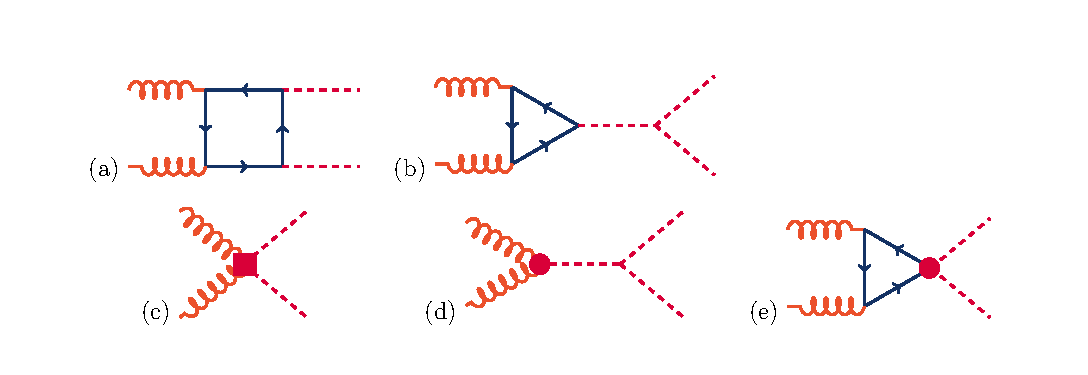
\includegraphics[scale=0.85]{figures/translation.pdf}
\caption{\small Feynman diagrams that contribute to Higgs boson pair production by gluon-gluon fusion at leading order. Diagrams (a) and (b) correspond to SM-like processes, while diagrams (c), (d), and (e) correspond to pure BSM effects: (c) and (d) describe contact interactions between the Higgs boson and gluons, and (e) exploits the contact interaction of two Higgs bosons with top quarks.   \label{fig:dia}}
\end{figure} 

In the Ref.~\cite{Dall'Osso:2015aia} it was designed a method to partition the 5 dimensional parameter space in regions 
with similar LO kinematics. 
When the simulation was launched in the CMS system this work was in preliminary version, we had simulated the samples 
referent to the recommendations of its first version. The list of relevant parameters iused in each sample is in table~\ref{tab:bench}. 
 The {\tt MG5\_aMC@NLO} configuration cards used for the simulations are organized here~\cite{cards}. 
Since then, the metric used by the method was improved and the parameter space scan extended, resulting in a 
new set of benchmarks, that can be found in the last ArXiV version of the mentioned paper, and as well in~\cite{MelladoGarcia:2150771}.


The full simulated samples can be found on DAS as:
\begin{itemize}
  \item \verb|/GluGluToHHTo2B2G_node_X_13TeV-madgraph|
\end{itemize}
where the $X$ ranges between 0 and 13. The $X=0$ represents the point ($\kappa_{\lambda}$, $\kappa_{t}$, $c_2$, $c_g$, $c_{2g}$) = (0,1,0,0,0) - when the process is induced only by the box diagram and the reminiscent correspond to the points listed in Tab.~\ref{tab:bench}.
The analytical formula that allows us to calculate cross sections for any point of the parameter space can be found here~\cite{CarvalhoAntunesDeOliveira:2130724}, and a handful script that calculates the cross sections point by point can be found here~\cite{hhrosetta}.  

%In Figure XX we show the Distributions at Gen level {\bf CHECK}.
In the next session we explain how we had derived results in different benchmark points, based in the above full-simulated samples. \\


\begin{table}
\centering
\small{
\begin{tabular}{|c||c|c|c|c|c|}
\hline
Node & $\kappa_{\lambda}$ & $\kappa_{t}$ & $c_2$ & $c_g$ & $c_{2g}$ \\\hline
1  &   1.0 & 1.0  &  0.0 &  0.0 &  0.0  \\ \hline
2  &   7.5 & 2.5  & -0.5 &  0.0    &  0.0      \\ \hline
3  &  15.0 & 1.5  & -3.0 & -0.0816 &  0.3010   \\\hline
4  &   5.0 & 2.25 &  3.0 &  0.0    &  0.0     \\\hline
5  &  10.0 & 1.5  & -1.0 & -0.0956 &  0.1240  \\ \hline
6  &   1.0 & 0.5  &  4.0 & -1.0    & -0.3780  \\ \hline
7  &   2.4 & 1.25 &  2.0 & -0.2560 & -0.1480  \\ \hline
8  &   7.5 & 2.0  &  0.5 &  0.0    &  0.0     \\ \hline
9  &  10.0 & 2.25 &  2.0 & -0.2130 & -0.0893  \\ \hline
10 &  15.0 & 0.5  &  1.0 & -0.0743 & -0.0668  \\ \hline
11 & -15.0 & 2.0  &  6.0 & -0.1680 & -0.5180  \\ \hline
12 &   2.4 & 2.25 &  2.0 & -0.0616 & -0.1200   \\ \hline
13 & -15.0 & 1.25 &  6.0 & -0.0467 & -0.5150   \\ \hline
\end{tabular}
}
\caption{\small Parameter values of the final benchmarks selected with $N_{clus} = 13$. 
The first cluster is the one that contains the SM sample. 
\label{tab:bench_old}}
\end{table} 

\mbox{}\\{\bf - Distributions at Gen level}

\subsubsection{Reweighting}
\label{sec:rewei}

We are considering a $2\to 2$ process at leading order. The two Higgs bosons are produced with identical transverse momenta ($p_{T}^{H}$), and they are back-to-back in azimuth at this order (before a parton shower). The final state can then be completely defined by three kinematic variables, if we ignore the irrelevant azimuthal angle of emission of the bosons. Furthermore, one of the three remaining variables can be used to isolate all the information related to the PDF of the colliding partons, which is also irrelevant to the physics of the production process once one focuses on a specific initial state (the gluon-gluon fusion process). The variable factorizing out the PDF modeling can be taken as the magnitude of the boost of the centre of mass frame as seen in the laboratory frame. 

The two remaining variables, which provide direct information on the physics of GF HH production, can be chosen to be the invariant mass of the HH system ($m_{HH}$) and the modulus of the cosine of the  polar angle of one Higgs boson with respect to the beam axis ($|cos\theta^*|$). Since we are using parton-level information, this last variable is equivalent to the polar angle in the Collins-Soper frame ($|cos\theta^*_{CS}|$)~\cite{PhysRevD.16.2219}, which is commonly used in experimental analysis. The variables $m_{HH}$ and $|cos\theta^*|$ can thus be used to fully characterize the final state kinematics produced by different choices of the value of anomalous Higgs boson (self-) coupling parameters.

By construction the full-simulated samples listed in Tab.~\ref{tab:bench}  are good representatives of the kinematic space. 
Therefore, based in the generation level $m_{HH}$ and $|cos\theta^*|$, those can be used to construct 
samples to any other parameter space point. 

The procedure is made as follows: 
\begin{itemize}
\item For each new parameter space point we perform 
a simulation in {\tt MG5\_aMC@NLO}, asking for $N$ events;
\item We construct two dimensional histograms in the 
generation level $m_{HH}$ and $cos\theta^*$, with 20$\GeV$-wide bins in the $m_{HH}$ and
 0.2-wide bins in $cos\theta^*$ (without the moduli);
\item We construct the same histogram with the sum of all the full simulated samples described in the last section (signal dataset);
\item The new sample is constructed by weigthing the signal dataset event-by-event by:
 \begin{equation}
 W_{e} = \frac{New_{ij}}{D_{ij}}\,,
 \end{equation}
 where ($ij$) specify the bin in which the event $e$ belongs and $New_{ij}$ ($D_{ij}$) the number of events of the 
 new signal sample (signal dataset) in that bin. 
 \end{itemize}
 
 We make reweighted samples for three types of theory scans:
\begin{itemize}
%  \item The frozen list of benchmarks of Refs.~\cite{Dall'Osso:2015aia,MelladoGarcia:2150771}, listed in Tab.~\ref{tab:bench}. 
  \item A plain scan in $\kappa_{\lambda}$, while all the other parameters are kept as in SM ($\kappa_{t}$, $c_2 = c_g  = c_{2g} =0$), where the gen-level histograms are made from 50,000 events
  \item Another set of samples that we will use to calculate the shape systematics necessary to extrapolate the limits in the benchmarks to an extended part of the parameter space (see Sec.~\ref{sec:shapesyst}).
\end{itemize} 
%The 2D histograms to construct the new samples are HERE and the map pf weights to the dataset BLA is HERE.
 
 \begin{table}[h]
\centering
\small{
\begin{tabular}{rccccc}
\hline
Benchmark & $\kappa_{\lambda}$ & $\kappa_{t}$ & $c_{2}$	& $c_{g}$ & $c_{2g}$ \\\hline
1 &	7.5	 & 1.0	 &	-1.0	& 0.0	& 0.0 \\
2 &	1.0	 & 1.0	 &	0.5		& -0.8	& 0.6 \\
3 &	1.0	 & 1.0	 &	-1.5	& 0.0	& -0.8 \\
4 &	-3.5 & 1.5  &	-3.0	& 0.0	& 0.0 \\
5 &	1.0	 & 1.0	 &	0.0		& 0.8	& -1 \\
6 &	2.4	 & 1.0	 &	0.0		& 0.2	& -0.2 \\
7 &	5.0	 & 1.0	 &	0.0		& 0.2	& -0.2 \\
8 &	15.0 & 1.0	 &	0.0		& -1	& 1 \\
9 &	1.0	 & 1.0	 &	1.0		& -0.6	& 0.6 \\
10 &	10.0 & 1.5   &	-1.0	& 0.0	& 0.0 \\
11 &	2.4	 & 1.0	 &	0.0		& 1		& -1 \\
12 &	15.0 & 1.0	 &	1.0		& 0.0	& 0.0 \\ \hline %cl no. 463
SM &	1.0 & 1.0	 &	0.0		& 0.0	& 0.0 \\
\hline
\end{tabular}
}
\caption{\small Parameter values of the twelve benchmarks and the Standard Model point.  \label{tab:bench}}
\end{table}
 
\subsubsection{Non-resonant Vector Boson Fusion}

For the 2016 version of the analysis, one non-resonant VBF sample was also produced centrally with the Standard Model coupling parameters. 
The MiniAOD version of this sample can be found on DAS under:   
/VBFHHTo2B2G\_CV\_1\_C2V\_1\_C3\_1\_13TeV-madgraph/RunIISummer16MiniAODv2-PUMoriond17\_80X\_mcRun2\_asymptotic\_2016\_TrancheIV\_v6-v1/MINIAODSIM
 
\subsection{Background MC}

Even though the signal extraction and background modeling of this analysis are performed based on data, background Monte Carlo samples are used to validate the simulation of our signal description and to develop the analysis. The main backgrounds for the $\bbgg$ final state come from either well-isolated photons coming from the hard scatter (prompt photons) or isolated photons reconstructed due to very collimated $\pi^{0}\to\gamma\gamma$ decays fragmented from jets (fake photons). These backgrounds are the same as the ones to the SM $\Hgg$ analysis, and a more complete description of the samples used can be found in the $\Hgg$ AN ~\cite{Hgg2015, Hgg2016}.

We can classify these backgrounds with respect to the number of prompt and fake photons in the selected diphoton candidate. The prompt-prompt background events are simulated with the Sherpa generator; it includes the born processes with up to 3 additional jets at LO accuracy as well as the box processes at LO. The prompt-fake and the fake-fake contributions are simulated with PYTHIA8, with a "Double-EM Enriched" filter\footnote{it requires a high $\pt$ and well isolated photon-like signal (electromagnetic activity) coming from photons, electrons, or neutral hadrons)} applied during production to improve the samples selection efficiencies. Additionally, a sample of Drell-Yan events decaying into electrons, simulated at NLO with AMC@NLO, is used, although its final contribution to the event yield is minimal due to the $M(\gamma\gamma) > 100 \gev$ selection cut.

\subsection{Data}

The data samples used in this analysis correspond to approximately $36.5$ fb$^{-1}$ of data collected in 2016, reconstructed with the 80X CMSSW release.


\section{Analysis objects and selection}
This analysis uses general purpose reconstruction of photons and jets, which have been described in previous sections. 
We have brief descriptions below, pointing out specific choices made for the analysis.

\subsection{Triggers And Pre-Selection}
\label{sec:trigger}
Exploiting the high online performance of the CMS ECAL to reconstruct photons and electrons, the dataset used in this analysis is constructed with a selection that requires two photons at High Level Trigger (HLT) level.

For the 2016 data taking period, the online strategy was based on a single HLT trigger path:
\begin{itemize}
\item HLT$\_$Diphoton30$\_$18$\_$R9Id$\_$OR$\_$IsoCaloId$\_$AND$\_$HE$\_$R9Id$\_$Mass90;
\end{itemize}

In order to achieve a good data/simulation comparison, a pre-selection that is tighter than the online selection is applied on data and Monte Carlo. This pre-selection is described on table \ref{tab:preselection}. It is based on shower shape variables ($R9$, the ratio between the energy deposited on a 3x3 ECAL crystal matrix around the most energetic crystal in the supercluster, and the supercluster energy), isolation variables (charged hadron isolation, CHI, the sum of all charged hadron particle flow candidates energies inside a cone of $\Delta R < 0.3$ around the photon axis), identification variables (H/E, the ratio between the photon's energy deposit on HCAL and on ECAL), and kinematic variables ($E_{T}$ and the photon supercluster $\eta$). Only events that have at least one diphoton candidate passing the pre-selection requirements are considered in the analysis.

 \begin{table}[h]
\centering
\small{
\begin{tabular}{rcc}
Requirements & Leading Photon & Subleading Photon \\ \hline
$E_{T}$ & $30 \gev$ & $20 \gev$ \\ \hline
$|\eta|$ & \multicolumn{2}{c}{ $< 2.5$ and outside $1.442  |\eta| < 1.566$ } \\ \hline
Shower shape and Isolation & \multicolumn{2}{c}{ $R9 > 0.8$ or CHI $< 20$ or CHI/$E_{T} < 0.3$} \\ \hline
Identification & \multicolumn{2}{c}{ H/E $< 0.08$} \\ \hline
\end{tabular}
}
\caption{\small Trigger based pre-selection applied on diphoton candidates.  \label{tab:preselection}}
\end{table}

The SM $\Hgg$ analysis provides scale factors and uncertainties related to those scale factors due to this HLT selection, which we also apply in the analysis and take into account in our final list of systematics. 

\subsection{Photons}
\label{sec:photons}

The kinematic requirements applied on the photons, after the diphoton candidates have passed through the event pre-selection (see Section ~\ref{sec:trigger}), are similar to the ones used in the SM $\Hgg$ analysis. The selection is as follows:
\begin{itemize}
\item Leading photon $E_{T} > 30 \GeV$, trailing photon $E_{T}>20 \GeV$;
\item Leading photon $E_{T}/\Mgg > 1/3$, trailing photon $E_{T}/\Mgg > 1/4$;
\item $100 < \Mgg < 180 \GeV$.
\end{itemize}
Additionally, a photon identification requirement is applied to the photons.

The photon identification requirement is based on a multivariate algorithm that combines information from the photon cluster shape in ECAL, as well as isolation variables. 
This requirement provides a signal-like photon efficiency of $90\%$ for photons both on the ECAL barrel and endcaps. 
The scale factors used to ensure data/MC agreement in the selection efficiency are also applied; these scale factors are calculated centrally at CMS. 
Additionally, an electron veto is applied to avoid background with electrons faking photons, with corresponding scale factors and uncertainties.

%=========== OLD ===========

%Currently (as of January 2016), the available samples processed by the $\Hgg$ group only have stored 
%their own training of the photon MVA ID. 
%We have chosen working points that ensure that the resonant low mass samples have 
%a $90\%$ efficiency both in the barrel and the endcap ECAL regions. 

%\begin{table}[h]
%\centering
%\begin{tabular} { | c | c | }
%\hline
%ECAL Region & Hgg MVA Selection \\ \hline
%EB & 0.07 \\ \hline
%EE & -0.03 \\ \hline
%\end{tabular}
%\end{table}

%Efficiencies of the leading photon to pass the ID criteria, as a function of the photon transverse energy, 
%are shown in Figure \ref{fig:Hgg-PhoID-eff}. 
%Only photons matched to gen-level prompt photons are used. 


%\begin{figure*}[thb]
%  \centering
%  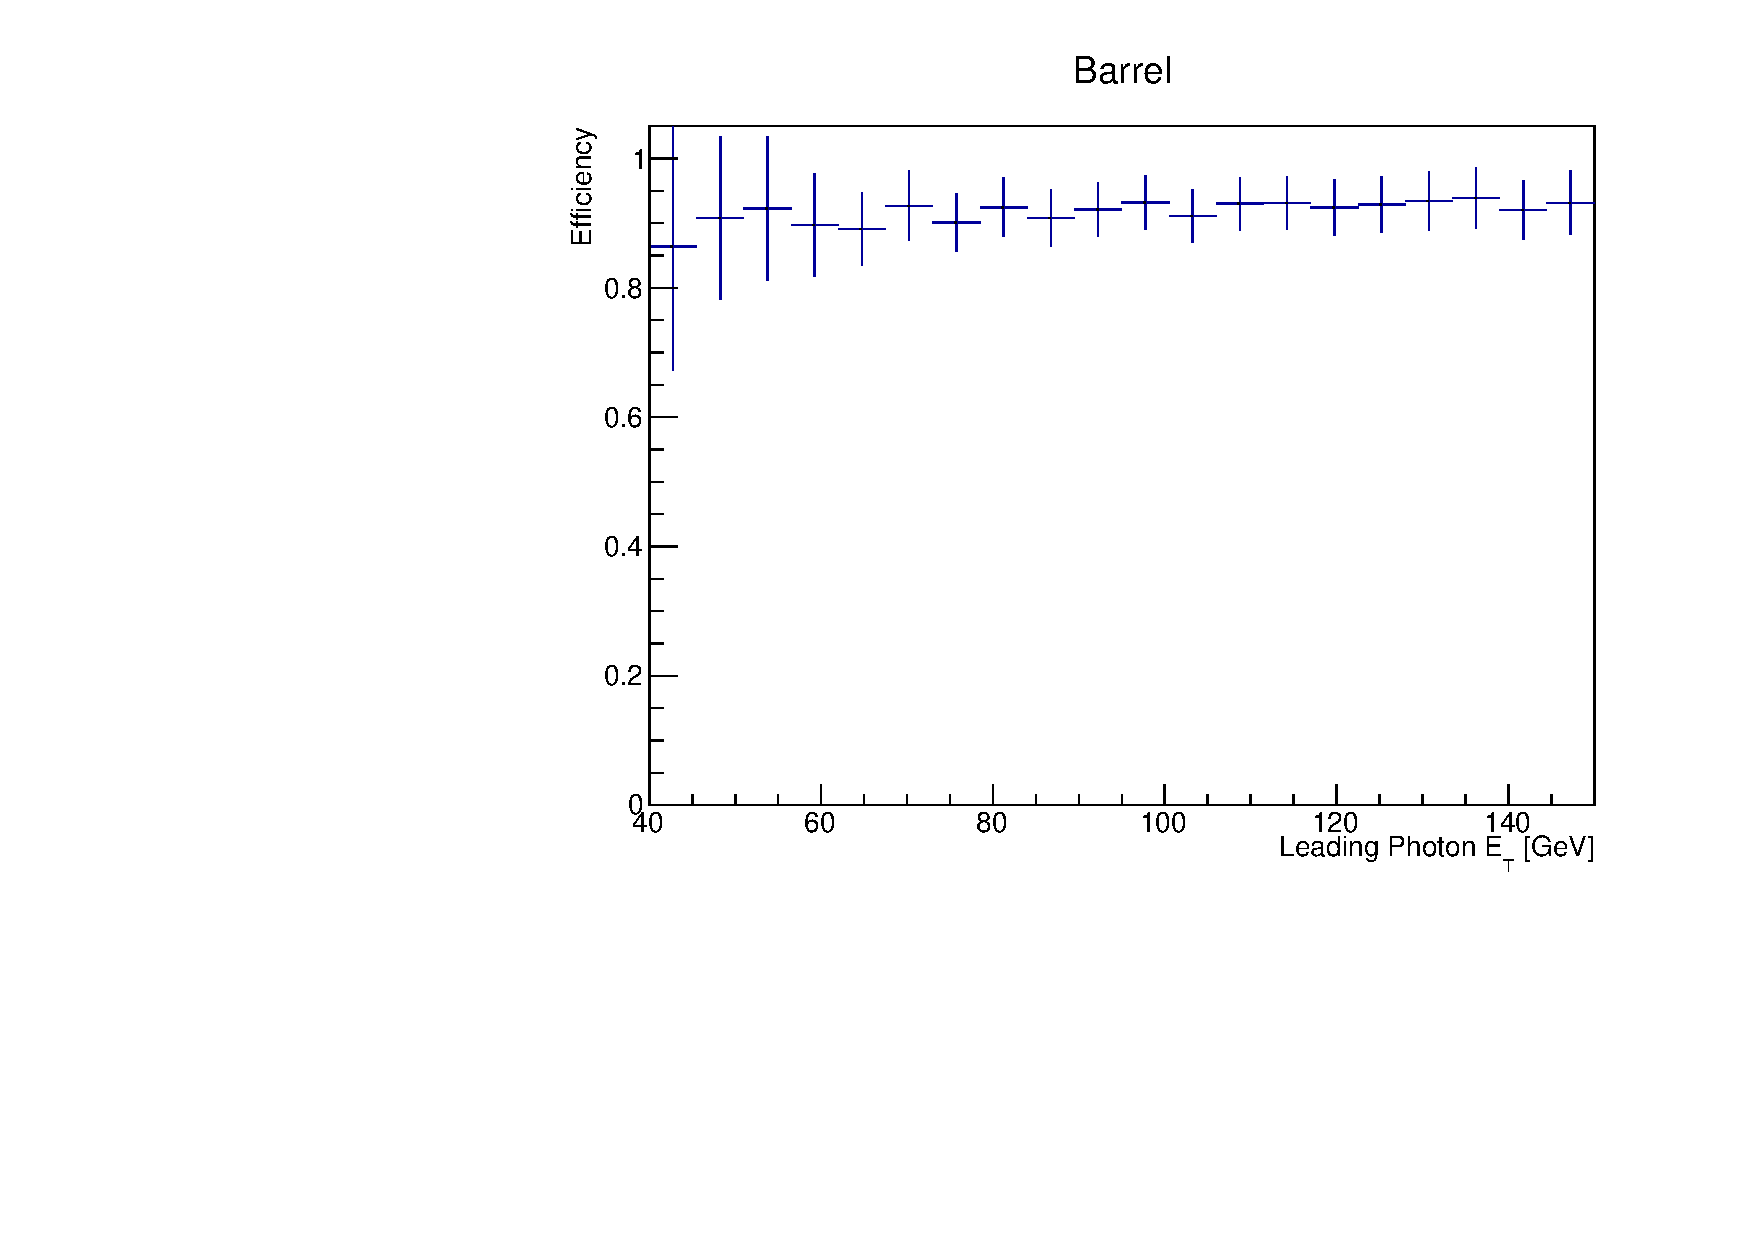
\includegraphics[width=0.45\textwidth]{figures/sec-photons/SMHH_HggMVA_Eff_EB.pdf}\hfil
%  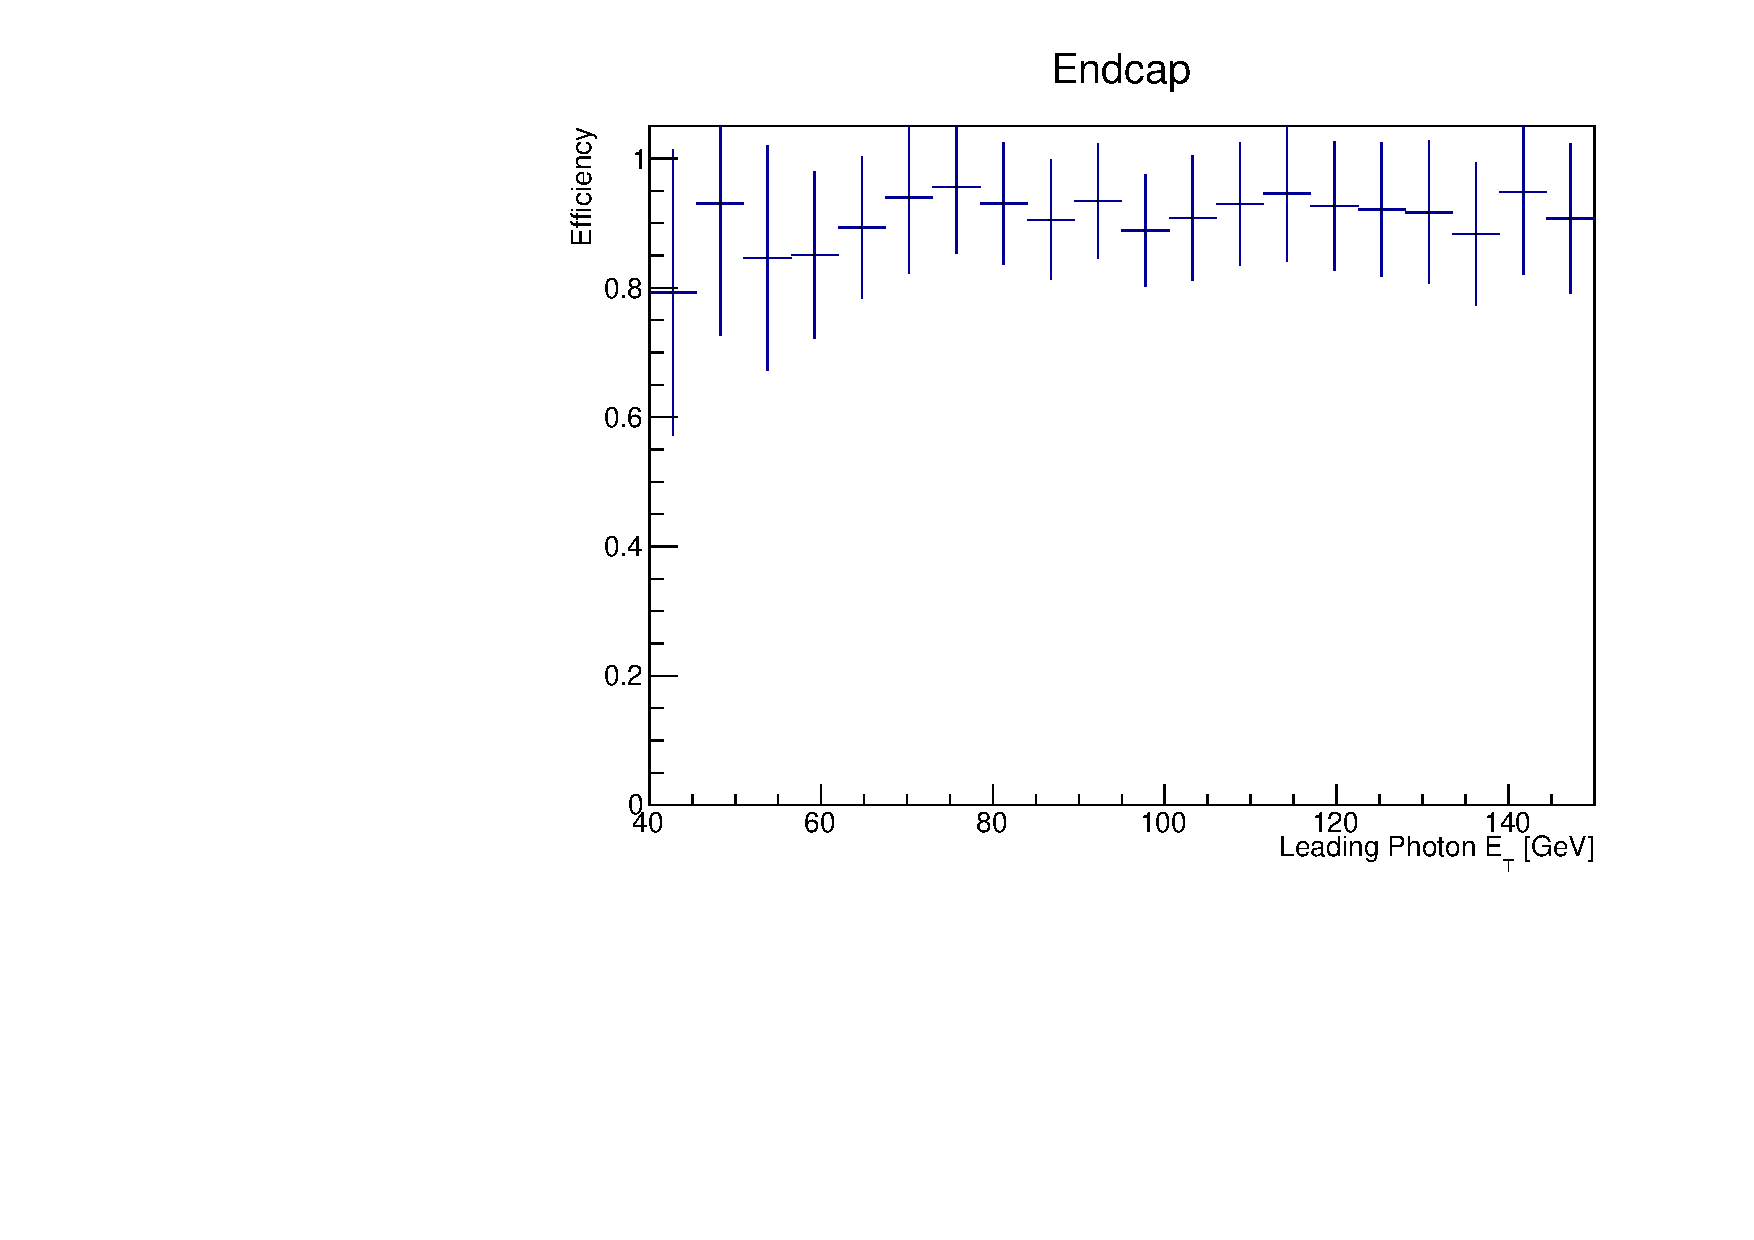
\includegraphics[width=0.45\textwidth]{figures/sec-photons/SMHH_HggMVA_Eff_EE.pdf}\hfil
%  \caption{Efficiencies of the leading photon to pass the ID criteria, as a function of the photon transverse energy, 
%for photons in the barrel and endcap regions of ECAL. }
%  \label{fig:Hgg-PhoID-eff}
%\end{figure*}

%We have studied all of those possibilities with MC samples, and for the 2015 data we
%decided to use the MVA ID of EGamma group with \textit{Loose} working point (WP),
%corresponding to 90\% signal selection efficiency.  A brief summary of this study is
%described below.

%The true photons are selected from the $G \to \HH \to \bbgg$ signal MC samples (they are
%required to match the generated level photons within $\Delta R< 0.1$ cone). The fake
%photons are selected from the Double-EM enriched $\gamma$+jet samples (and they must not
%to match to any generated level photon).
%The studied photons must pass the standard photon selection (pre-selection plus kinematic selection).

%Finally, the MVA score is calculated for the selected photons (or an ID decision for the
%cut-based ID).  Figure \ref{fig:phoID-MVA} shows two examples of the MVA output from the
%signal and fake photons. And Figure~\ref{fig:phoID-ROC} shows the ROC curves for the three
%IDs considered, for photons in the Barrel and Endcap. On these curves at a given signal
%efficiency one would prefer to have highest background rejection. From this figure of
%merit the MVA IDs are undoubtedly better than the cut-based ID. While the two MVA IDs have
%very similar performance.

%Note: it is anticipated that for 2016 data-taking the two MVA IDs will merge into one, and we
%will use that.

%\begin{figure*}[thb]
%  \centering
%  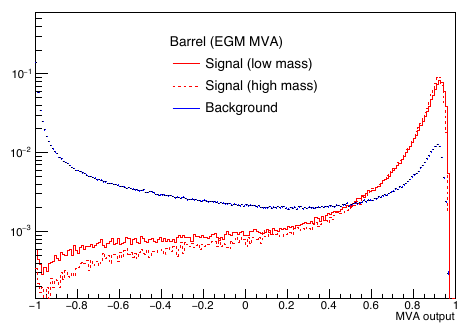
\includegraphics[width=0.45\textwidth]{MVA_output_EGM_Barrel}\hfil
%  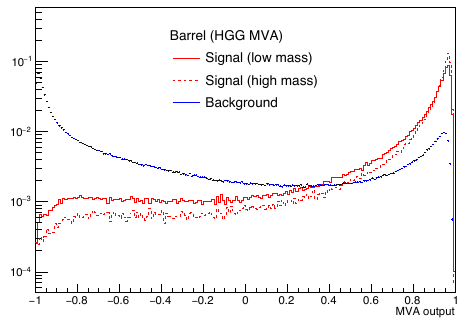
\includegraphics[width=0.45\textwidth]{MVA_output_HGG_Barrel}\hfil
%  \caption{Examples of the MVA ID outputs for the photons in the Barrel. Left: EGamma,
%    right: Hgg.}
%  \label{fig:phoID-MVA}
%\end{figure*}


%\begin{figure*}[thb]
%  \centering
%  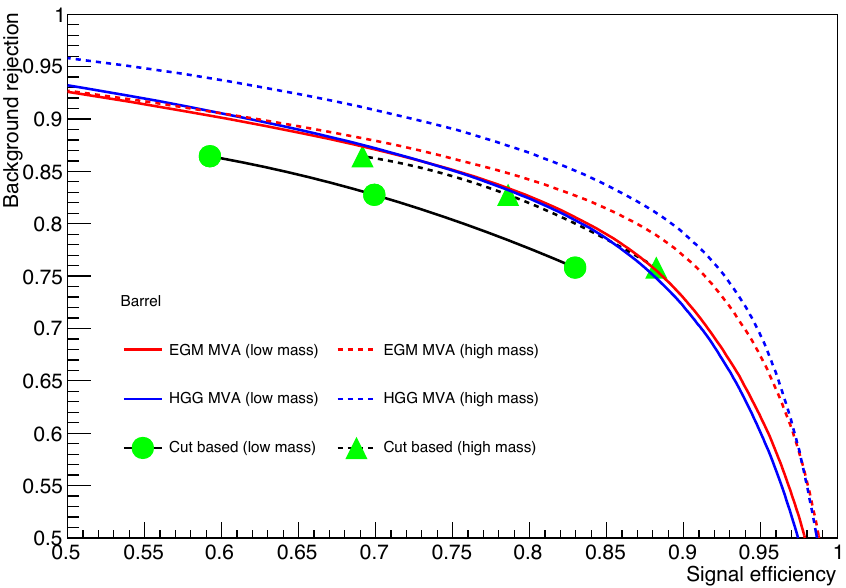
\includegraphics[width=0.45\textwidth]{ming_phoID_EB}\hfil
%  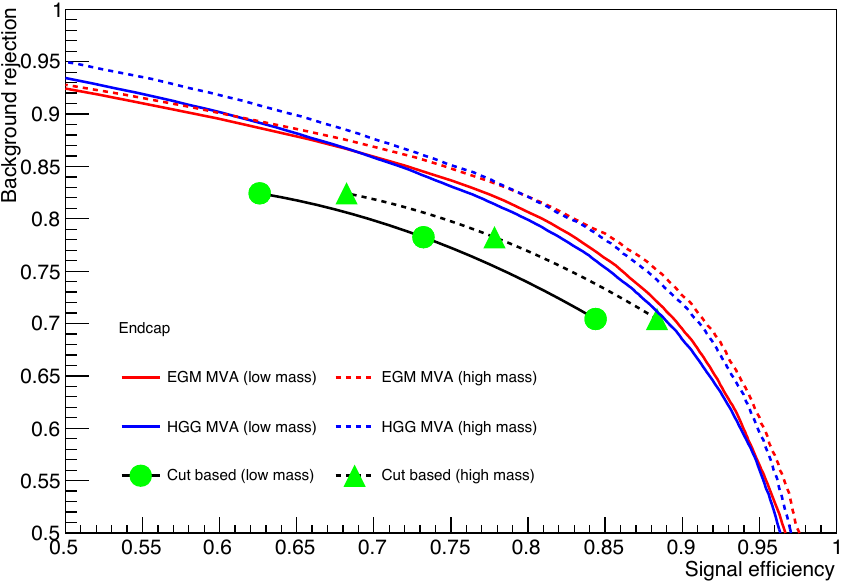
\includegraphics[width=0.45\textwidth]{ming_phoID_EE}\hfil
%  \caption{Photon ID ROC curves}
%  \label{fig:phoID-ROC}
%\end{figure*}

\subsubsection{Fake Photon Control Region}\label{sec:PCR}
A control region is created by selecting diphoton candidates with one photon that passed the ID requirement and one that didn't. All the other selections remain the same, and the procedure to select such diphoton candidates is the same as in the signal region. This control region is used in the analysis to perform closure tests on the background modeling.

\subsubsection{Vertex}
Inheriting from the main $\Hgg$ analysis, we use the vertex that gives the highest $\Hgg$ vertex MVA score. 
Because there are additional jets in the event,  picking this vertex has a very small mismatch efficiency. 
Only in less than $0.1\%$ of the events, the chosen vertex is different from the vertex associated to the true vertex in the simulation. 

The $\Hgg$ vertex MVA score is based on three variables calculated for each reconstructed vertex: the sum of the squared transverse momenta of the charged particle tracks associated with the vertex, and two variables that quantify the vector and scalar balance of $p_{T}$ between the diphoton system and the charged particle tracks associated with the vertex. 
In addition, if either photon is associated with any charged particle track that has been identified as resulting from conversion, the conversion information is also used. 
The variables are used as the inputs to a multivariate classifier based on a boosted decision tree (BDT) to choose the reconstructed vertex to be associated with the diphoton system. 
The average vertex finding efficiency of this algorithm in the SM $\Hgg$ analysis is $80\%$.

\subsubsection{Gain Switch}

In 2016, it was observed that high energy deposits in ECAL had their energies reconstructed with a certain bias, due to the shaping of the pulses in the ECAL VFE electronics. 
This shaping became a problem in Run 2 because we assume a certain shape for the signal amplitude from the crystals when measuring this amplitude, as described in the Multifit method. 
It has been observed that this bias occurs when an energy deposit is high enough to cause a gain switch in the ECAL multi-gain amplifier.

We investigated the fraction of selected events in our blinded signal region with photons that go through gain switches. 
The plots on Figure \ref{fig:gain_switch}  show, in bins of $\tilde{M}_{X}$, the fraction of events with at least one of the photon candidates going through gain switches (to gain 1, gain 6 or both). 
These results show that, for the high mass region, around $20\%$ of our events are affected by gain switches. 
This non-negligible rate means that the analysis needs to use the new CMS re-processed data in which the issue has been fixed.

\begin{figure*}[thb]
  \centering
%  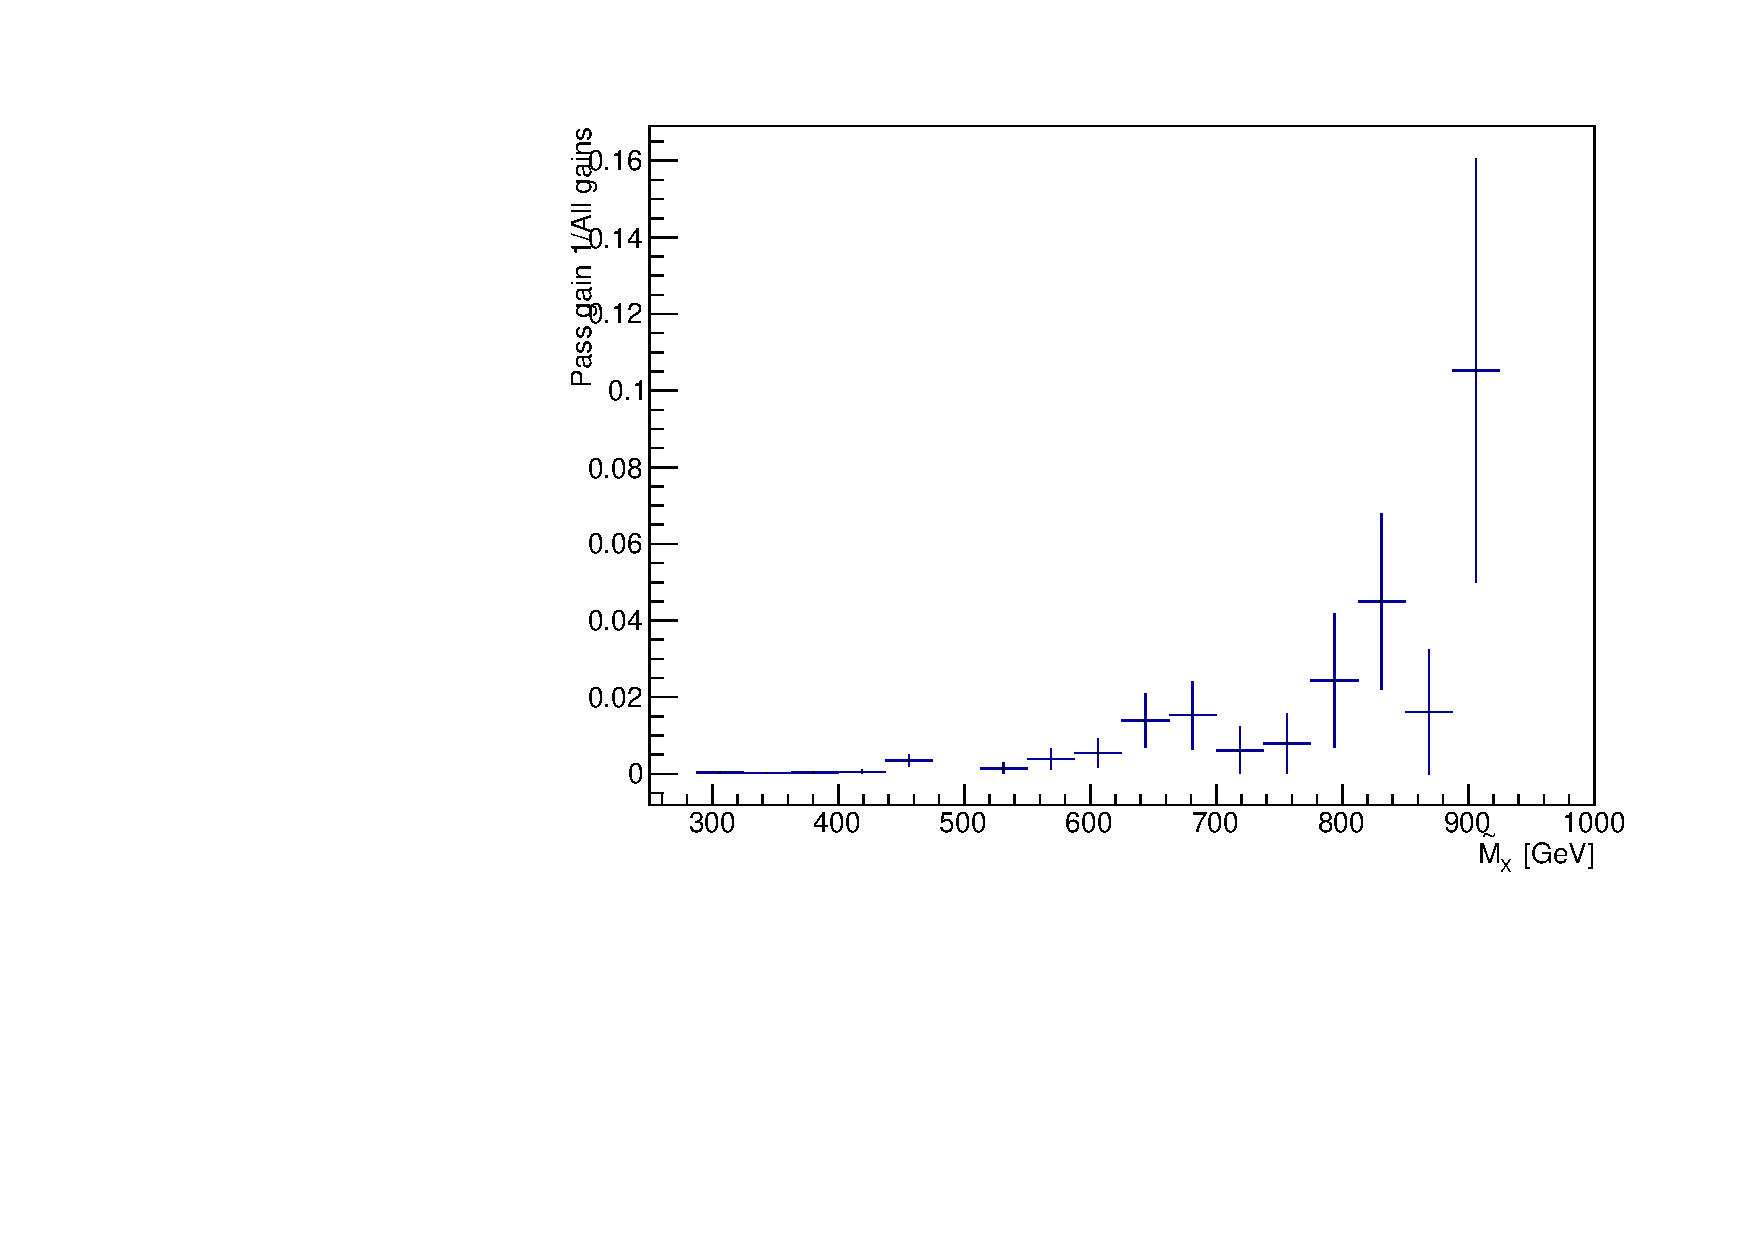
\includegraphics[width=0.3\textwidth]{figures/sec-photons/rg1}\hfil
%  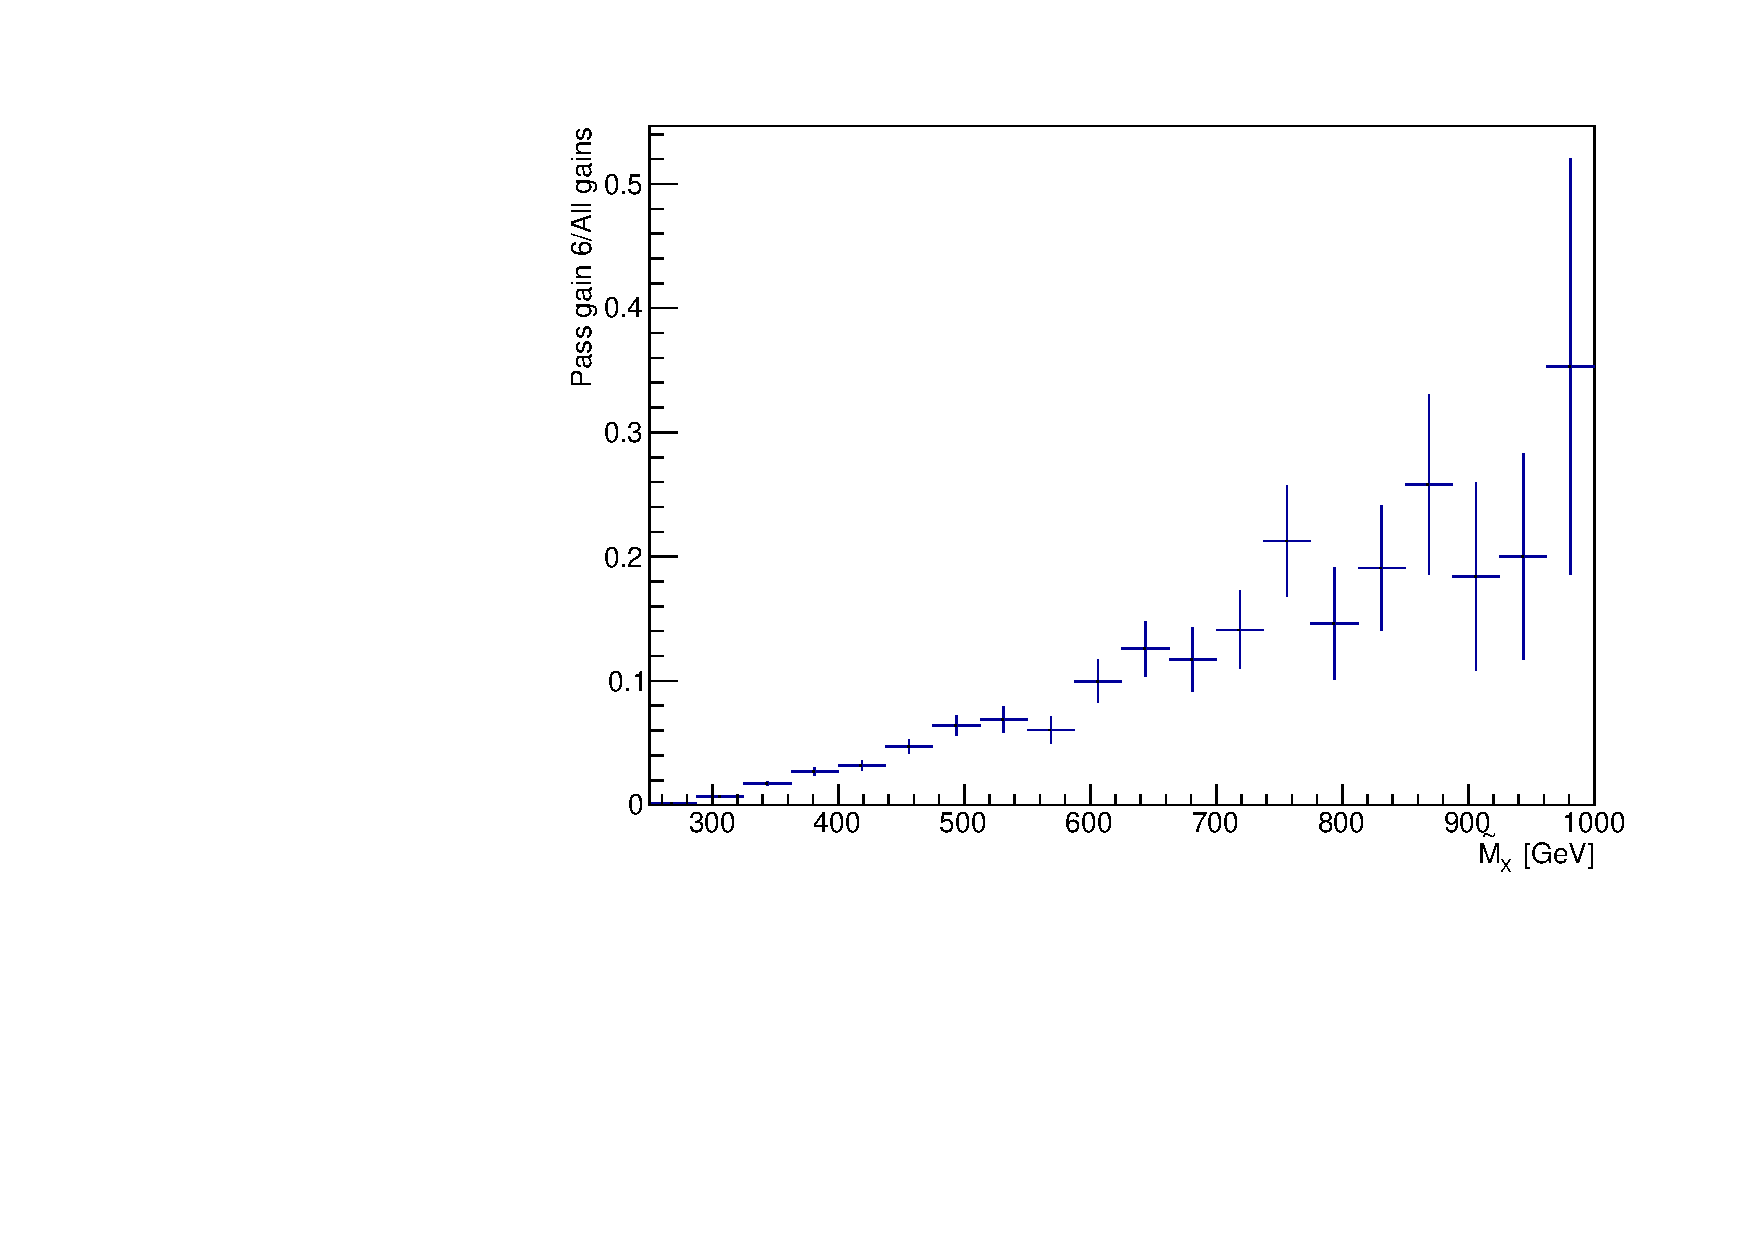
\includegraphics[width=0.3\textwidth]{figures/sec-photons/rg6}\hfil
  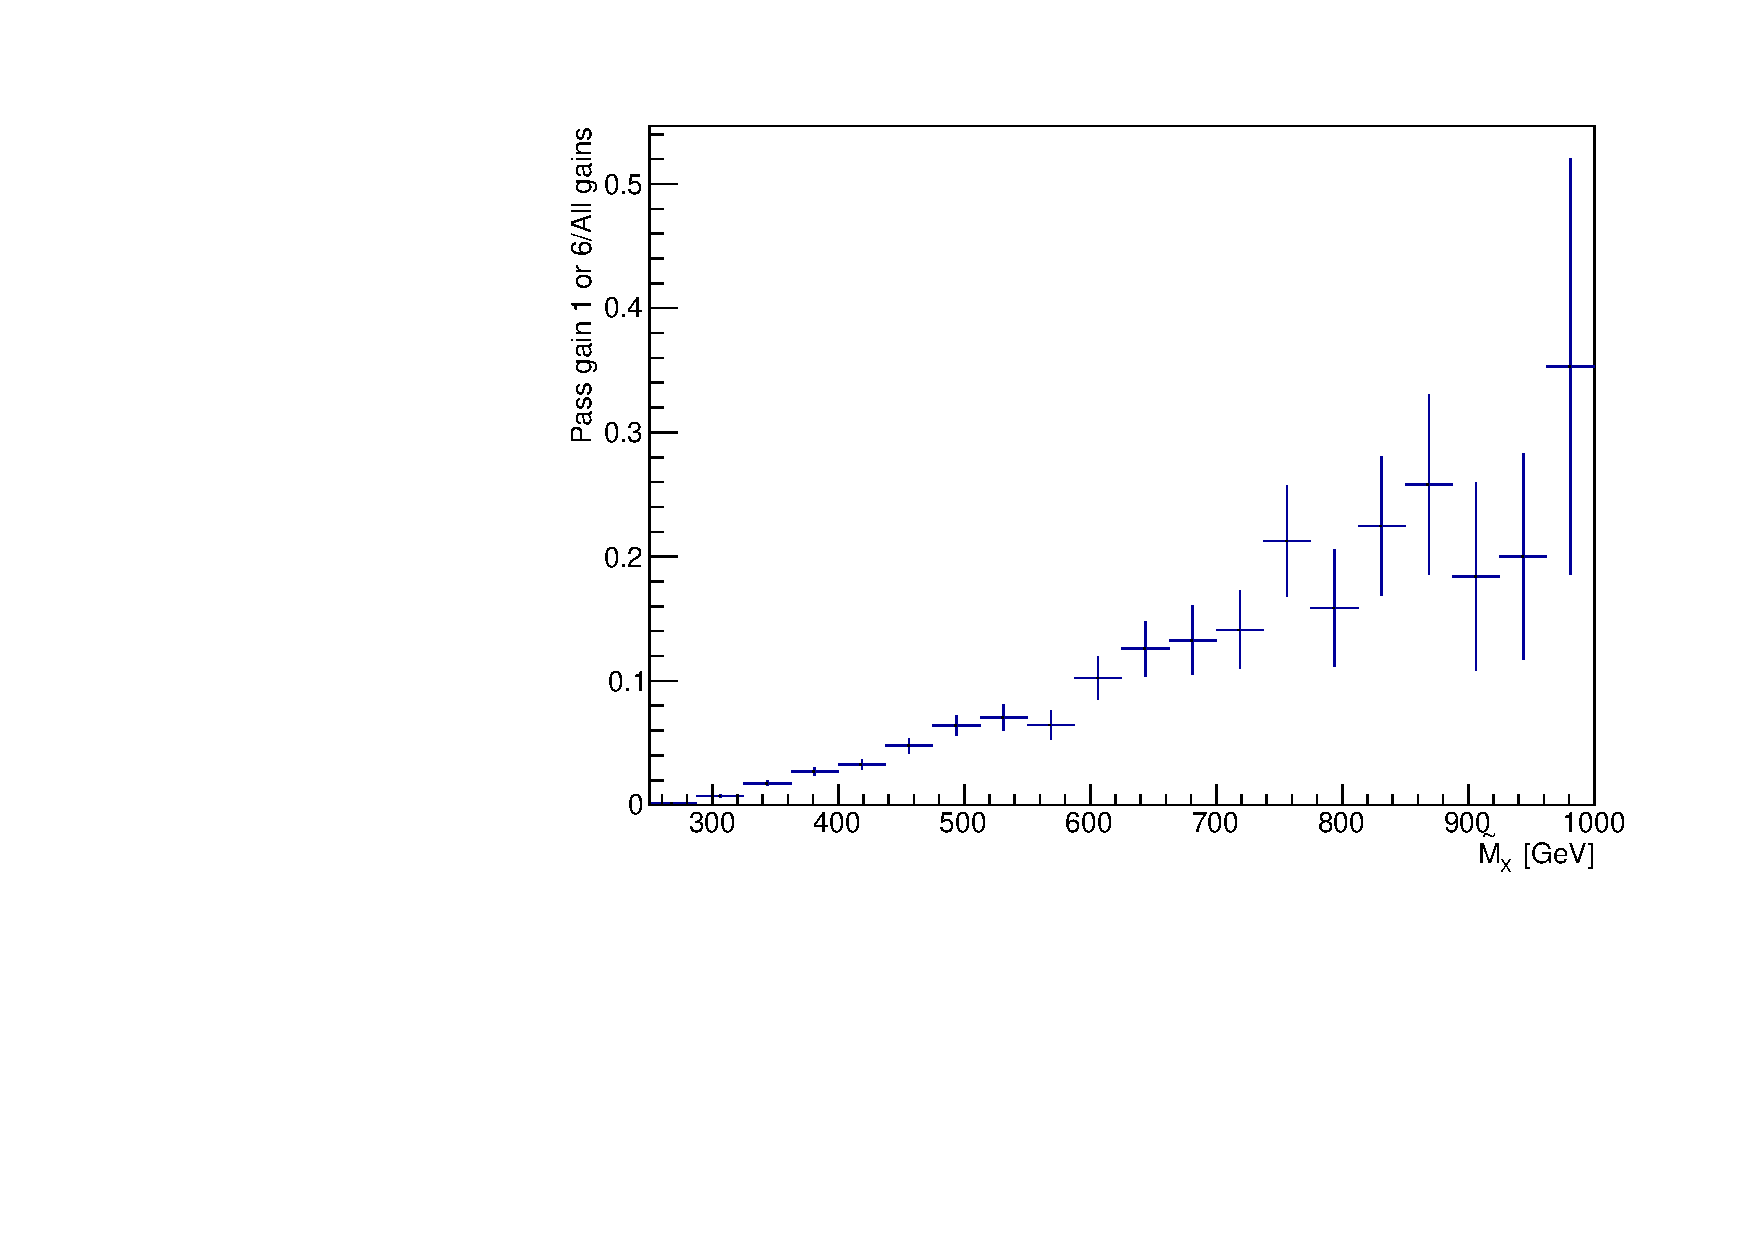
\includegraphics[width=0.5\textwidth]{figures/sec-photons/rg16}
  \caption{Fraction of events with photon candidates going through gain switch.}
  \label{fig:gain_switch}
\end{figure*}

\subsubsection{Regression}

A new version of the photon energy regression has been trained with the Run 2 data taking conditions. 
This regression aims to correct the photon super cluster energy, as described in previous sections.  
We compared this new regression to the previous training, as seen in the plots of Figure \ref{fig:pho_reg} for three different resonance mass points. 
The difference observed is not large enough for this analysis to be affected, so the previous regression version is used (following main $\Hgg$ analysis).

\begin{figure*}[thb]
  \centering
  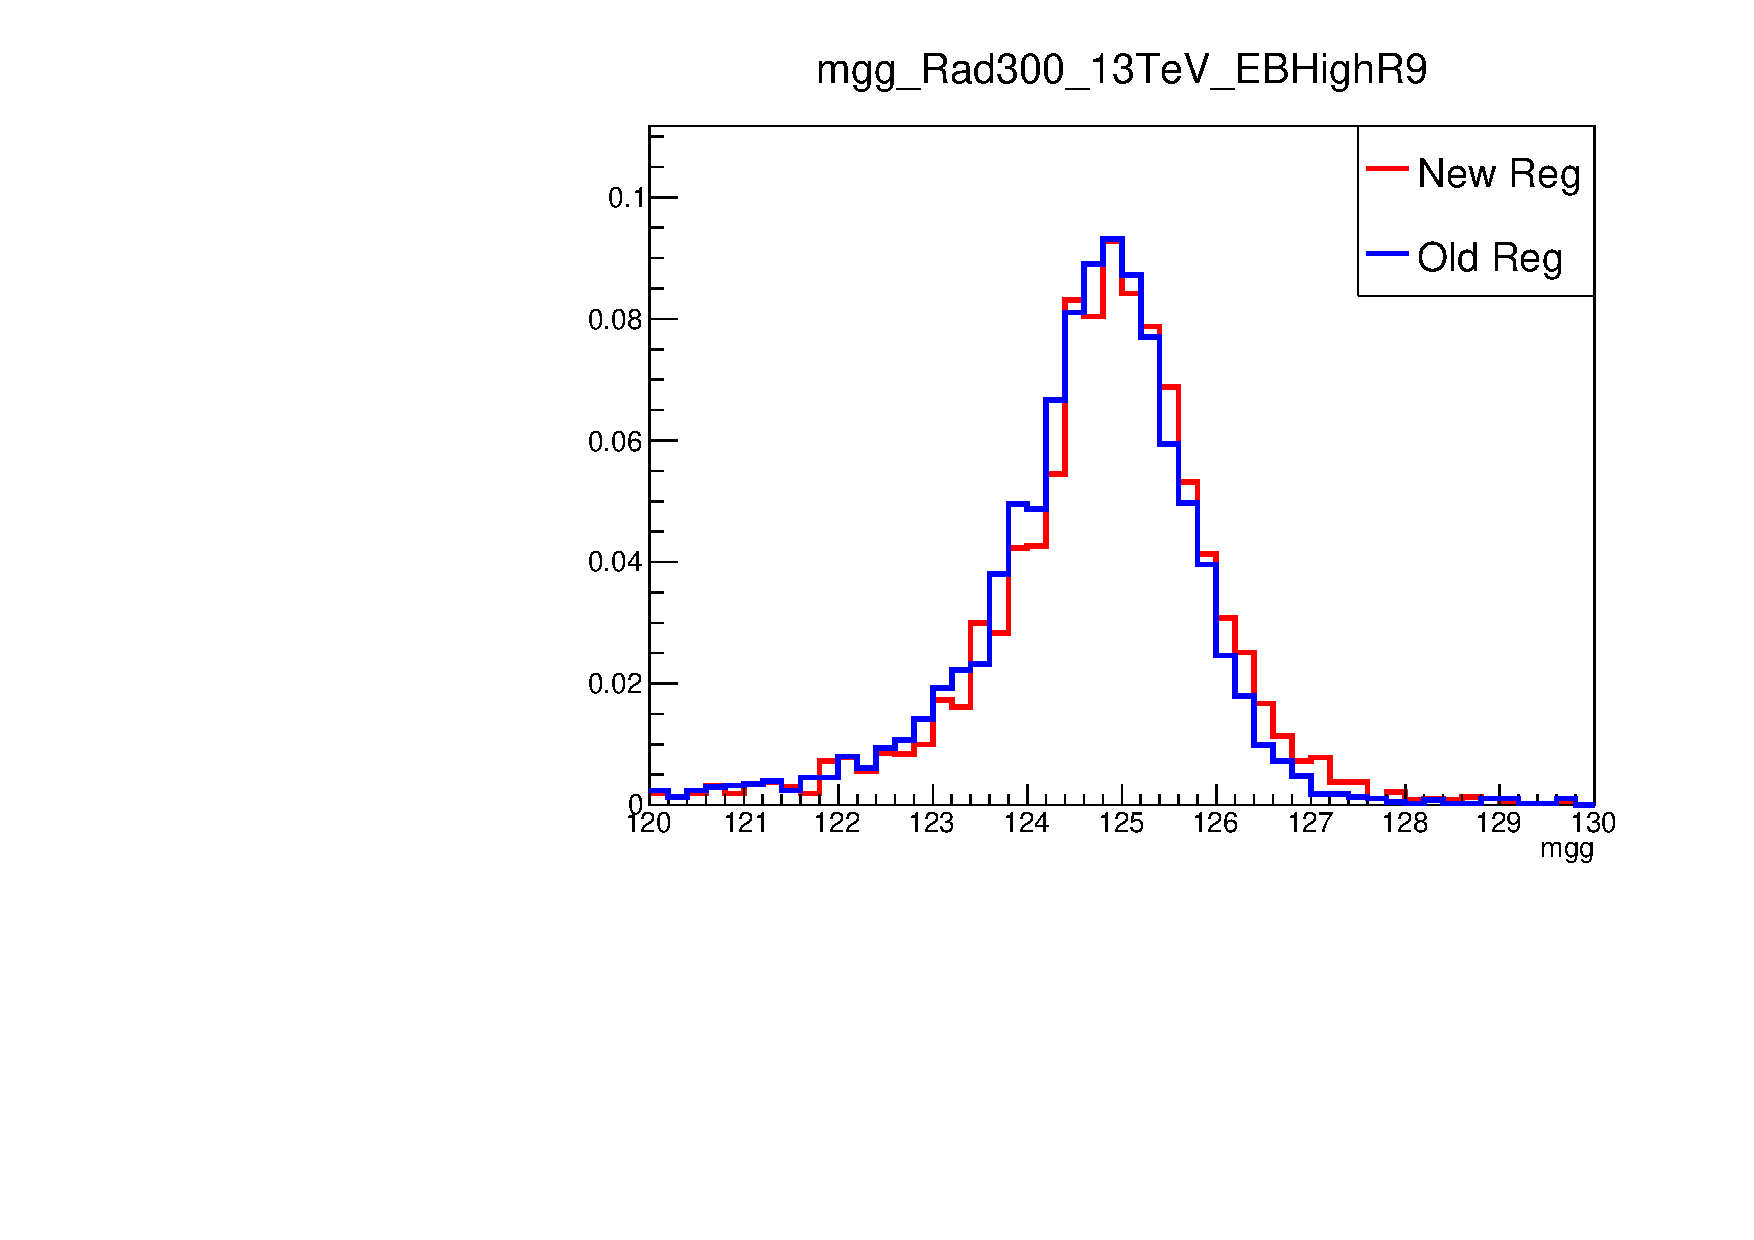
\includegraphics[trim={0 0 0 0.95cm},clip,width=0.3\textwidth]{figures/sec-photons/mgg_Rad300_13TeV_EBHighR9.pdf}\hfil
  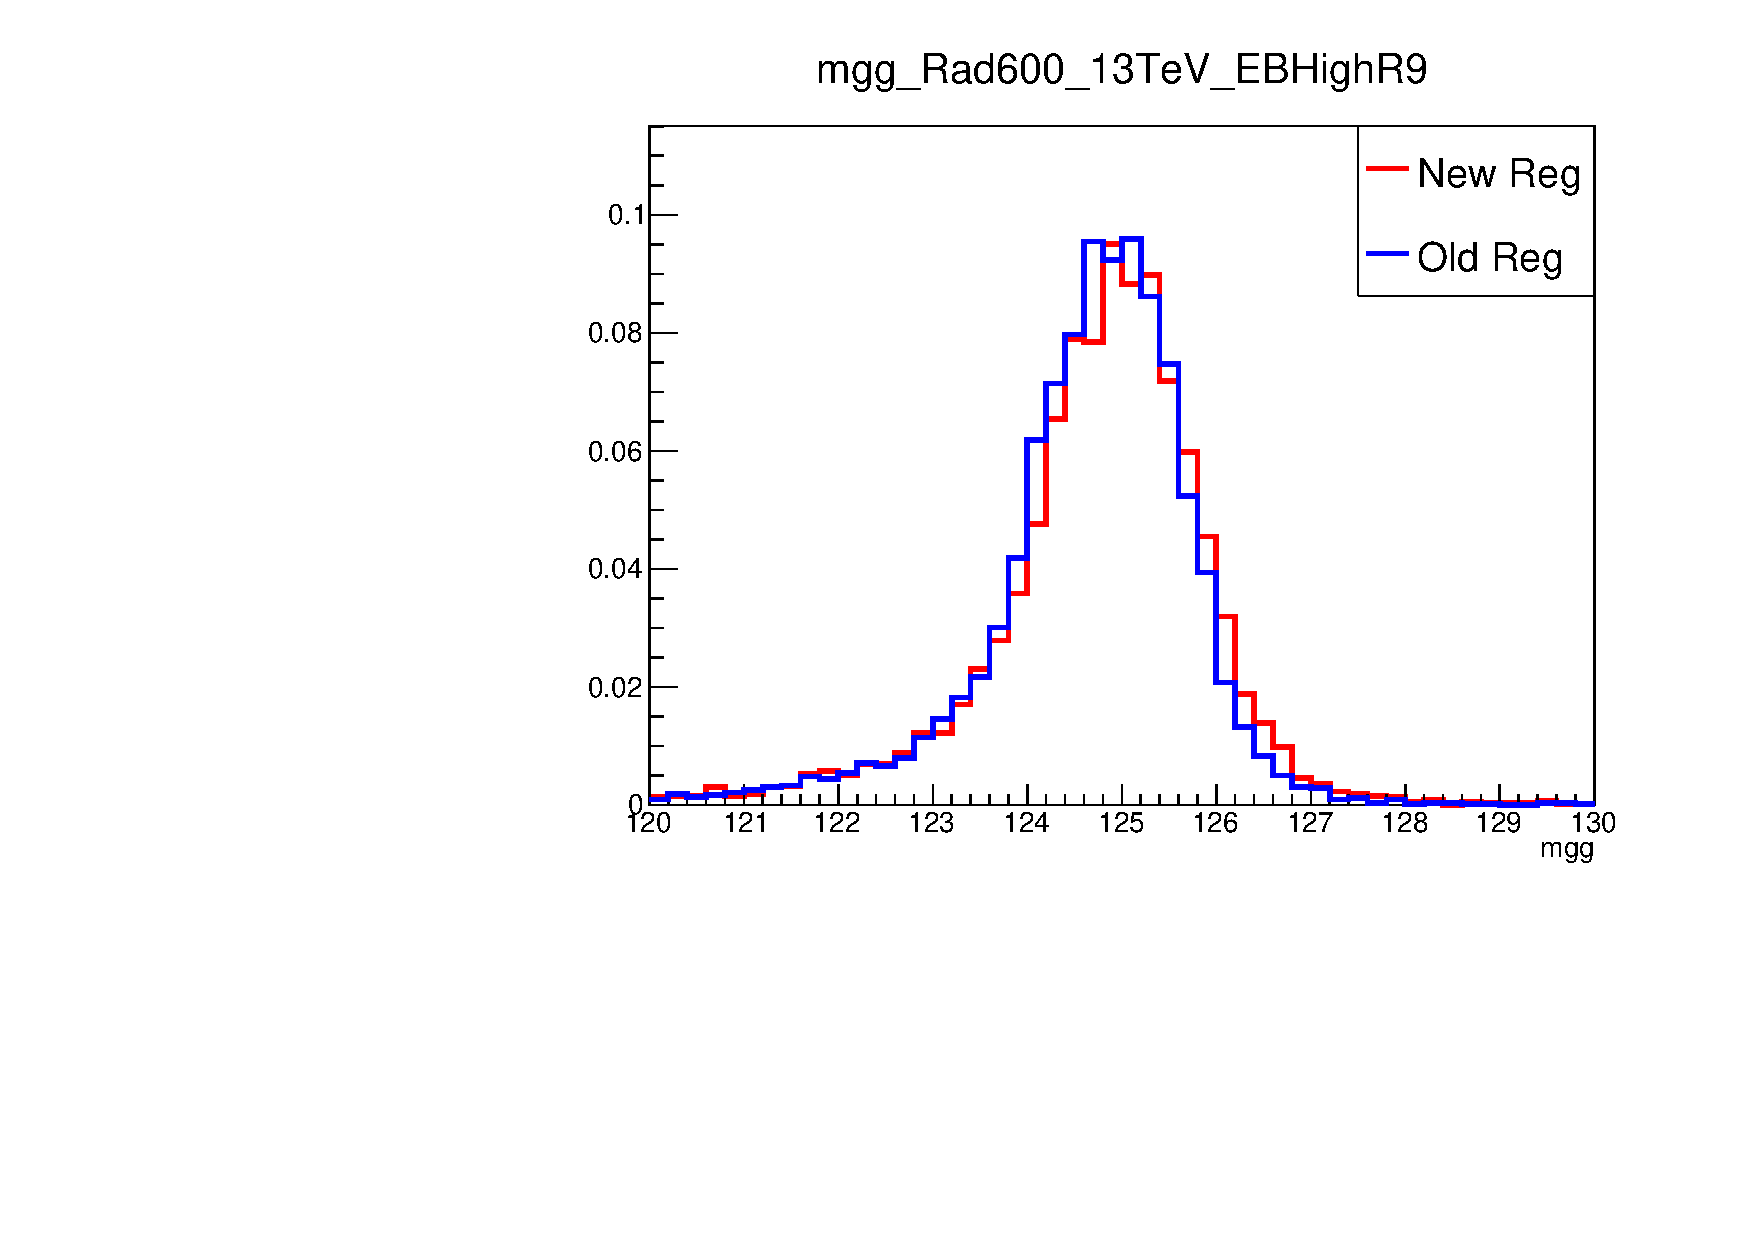
\includegraphics[trim={0 0 0 0.95cm},clip,width=0.3\textwidth]{figures/sec-photons/mgg_Rad600_13TeV_EBHighR9.pdf}\hfil
  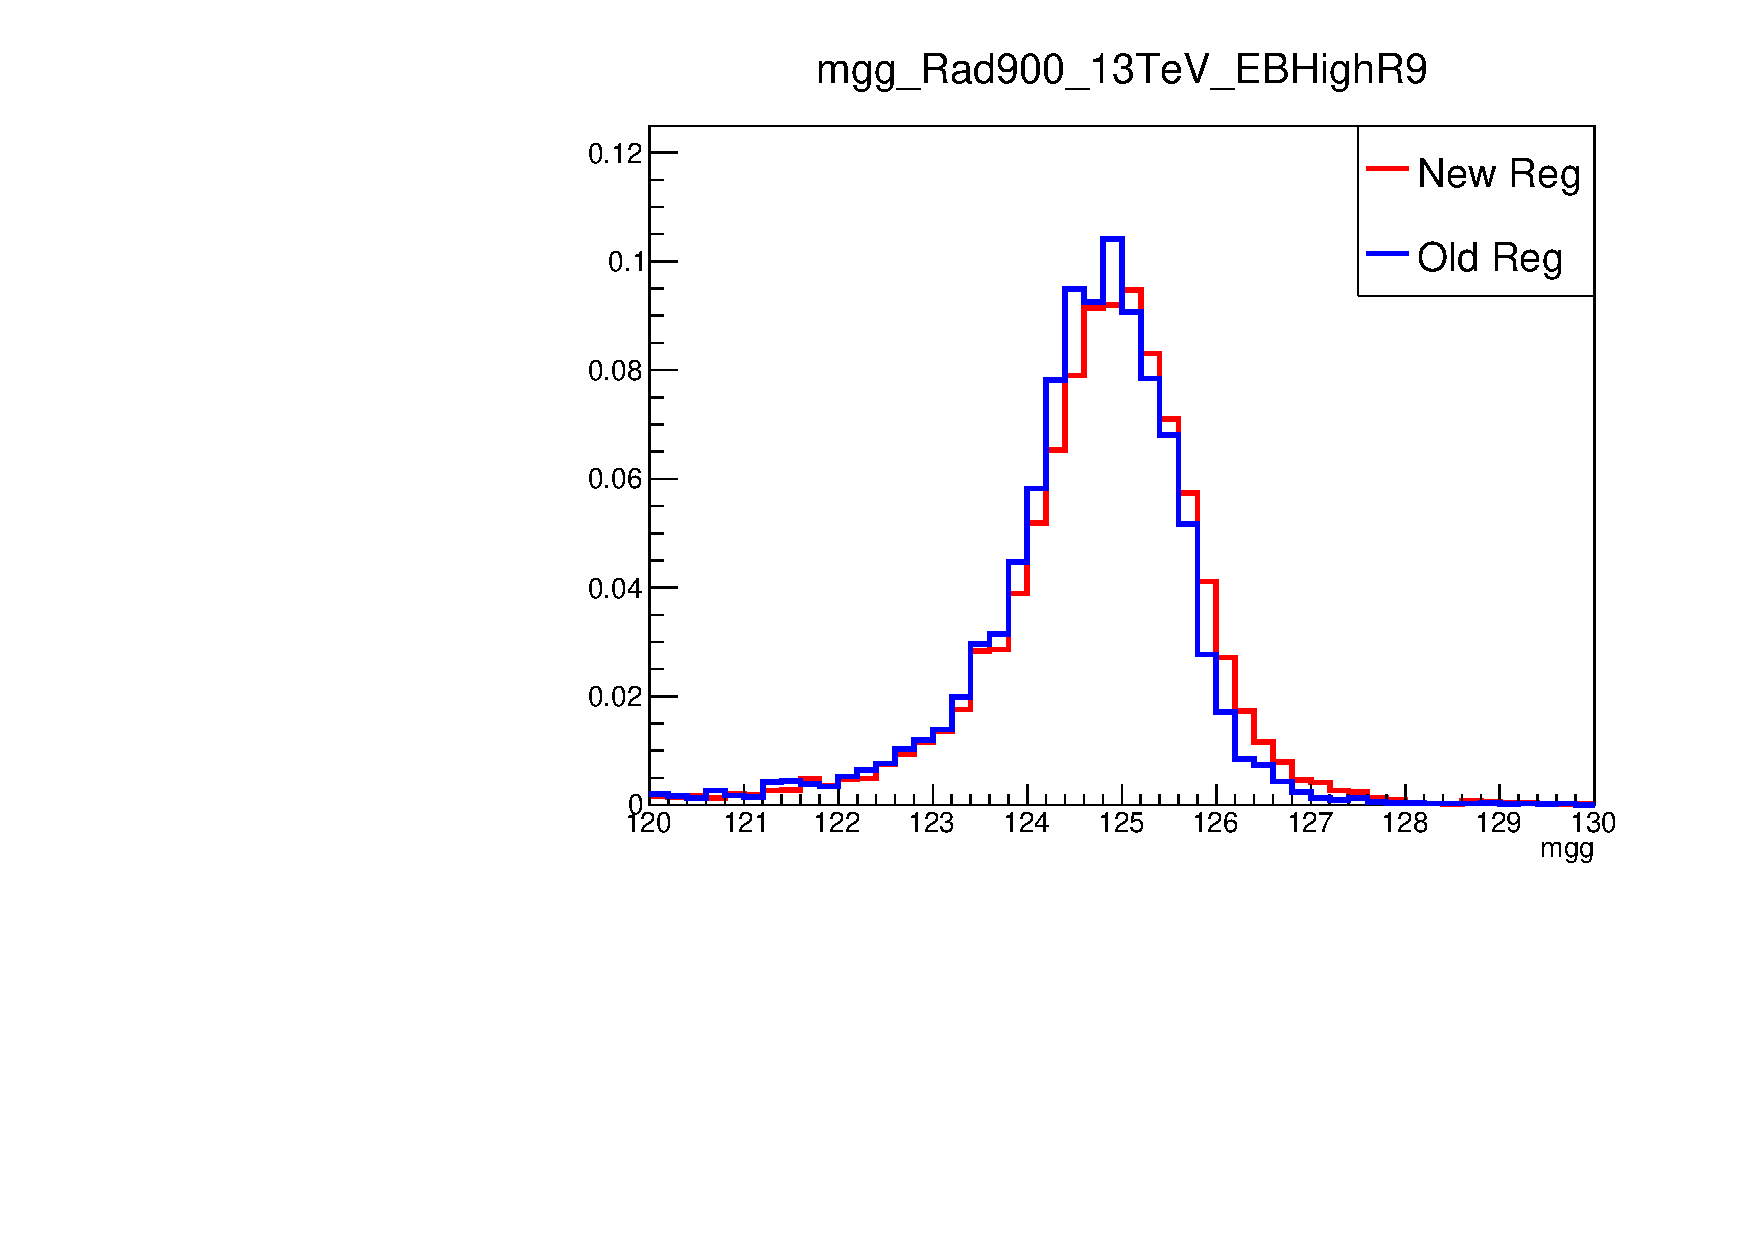
\includegraphics[trim={0 0 0 0.95cm},clip,width=0.3\textwidth]{figures/sec-photons/mgg_Rad900_13TeV_EBHighR9.pdf}\hfil
  \caption{$M(\gamma\gamma)$ reconstructed with different versions of the photon energy regression for resonance masses of 300, 600 and 900 GeV, from left to right. Distributions normalized to unity.}
  \label{fig:pho_reg}
\end{figure*}

\subsection{Jets}
\label{sec:jets}

The jets in Run-II at CMS are reconstructed using anti-kt algorithm
with the distance parameter $R=0.4$. This was a change with respect to
the parameter distance of $R=0.5$ in Run-I due to increased pile-up in
Run-II data taking. This change resultes in smaller $\Mjj$ resolution
but induced a bias towards lower energy of the signal $\Mjj$ peak,
because less energy is clustered in a jet. This effect can be seen in
figure \ref{fig:jet-reco} of the $\Mjj$ distribution for reconstructed
jets matched to generator-level jets (that come from the Higgs) from
the Radion sample of $M=300\GeV$.

\begin{figure*}[h]
  \centering
  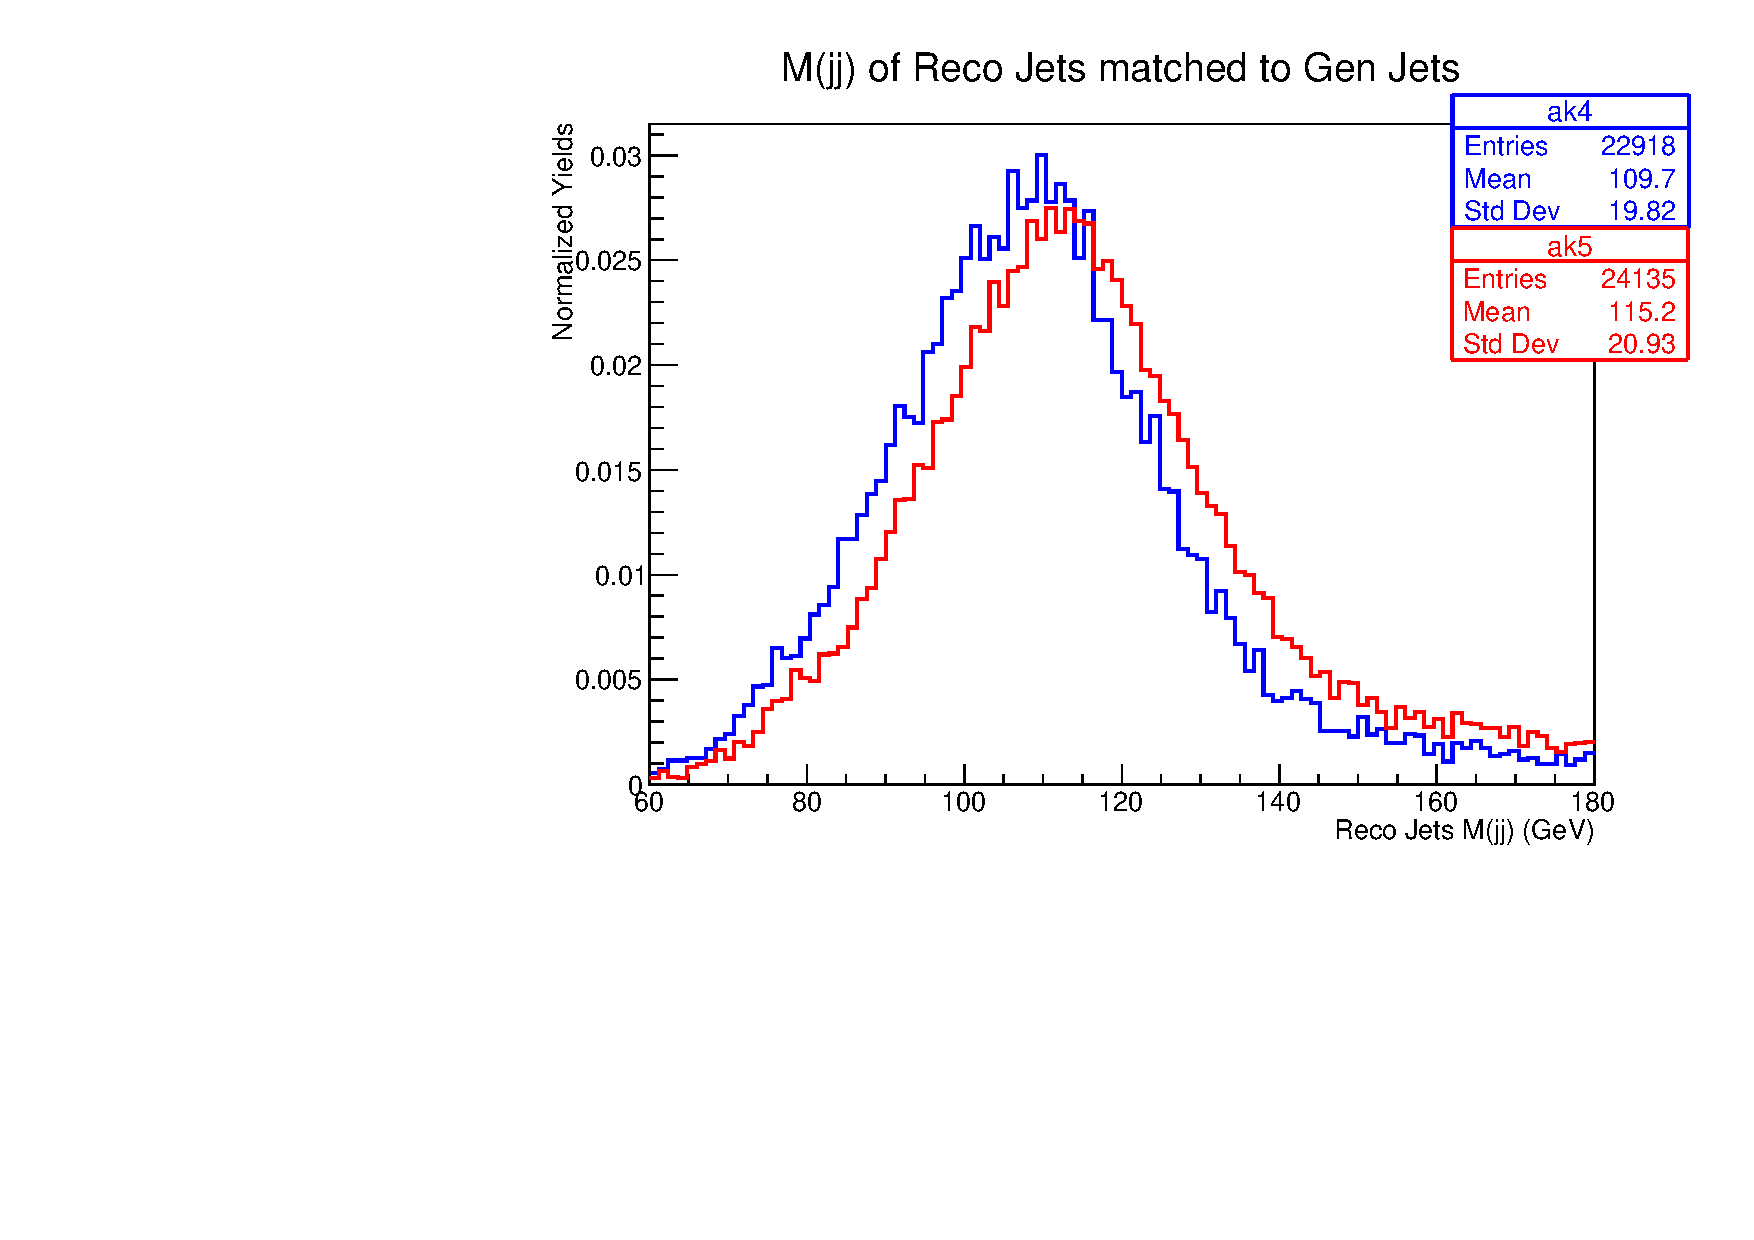
\includegraphics[width=0.45\textwidth]{figures/sec-jets/jet_rec.pdf}\hfil
  \caption{Difference between jet reconstruction used in Run I (red) and Run II (blue)}
  \label{fig:jet-reco}
\end{figure*}

We use the \textit{Loose ID} criteria to select the jets, which is described in
Ref~\cite{jetID-twiki}.

The jet candidates in the event, after passing the aforementioned ID,
must have $\PT > 25 \gev$ and $|\eta| < 2.4$ (so that they are within
the tracker of CMS and can be tagged as coming from $b$ quark). The
jets must also be outside the photon cone with a $\Delta R(j,\gamma) >
0.4$. Dijet objects are then created and only dijets with $\Mjj$ between 60 and 180 GeV 
pass the selection. If more than one dijet has passed those criteria, the dijet with two jets
with highest b-tagging score (see sec. \ref{sec:btag}) are selected as
the dijet candidate.


\subsection{Jet energy regression}
\label{sec:b-reg}

In addition to the misfortune of a small distance parameter of the jet reconstruction algorithm, the energy of the jets coming from $b$-quarks can not be fully reconstructed due to neutrinos escaping the detector. 
In order to improve the \Mjj resolution and gain in S/B discrimination, we employ an energy regression technique on our signal jets. 
The regression technique will work by changing the jet 4-momentum based on the likelihood that this specific jet is a signal jet. 

We use the TMVA package to implement the regression, and it on $X\to\HH\to\bbbb$ MC samples, in order to ensure a statistically independent training. 
Input variables to the training include jet kinematics, energy deposited in the calorimeter, vertex information, and variables related to missing transverse energy of the event (MET) and the distance between the two jets, $\Delta R(j,j)$. 
A summary of all input variables is shown in Table~\ref{tab:reg-vars}.

\begin{table}[h]\centering
\begin{tabular}{rl}
\hline
Input variables        & Jet kinematics: $\eta$, $\PT$, $m_T$\\
as in $\Hbb$ analysis  & Neutral hadron energy fraction, Photon energy fraction\\
regression:       & SecVtxdL, SecVtxdeL, SecVtxPt, SecVtxM, SecVtxNtrk\\
                  & Soft Lepton: \PT, \PT(rel), \DR \\
                  & \PT(Lead Track), Number of verteces\\\hline
\hline
Additional         & \\
variables for our  &\MET, $\Delta\phi(Jet, \MET)$, $\Delta R$(Leading jet, Trailing jet) \\
analysis:          & \\
\hline
\end{tabular}
\caption{Input variables used in TMVA regression. Upper part lists the
  variables that are also used in $\Hbb$ analysis, and the lower part
  lists additional variables.}
\label{tab:reg-vars}
\end{table}

The target for the regression training is $\PT^{gen}/\PT^{reco}$, where the generated level jet ("gen") contains neutrinos. 
This means that the regression technique will aim to construct, in a piece-wise manner, a function $f(\bar{x}) = \langle \PT^{gen}/\PT^{reco} \rangle (\bar{x})$, where $\bar{x}$ are the regression input variables, which can be used to correct the jet's energy. 
The standard gen-jet collection in CMS does not include the neutrinos, so we add them manually from gen-particle collection, using $\DR$ cone of 0.4 for matching.

Adding neutrinos to the gen-jet brings the energy of the jet closer to the energy of original b-quark, which is illustrated in Fig.~\ref{fig:b-reg-quark}.  
Figure~\ref{fig:b-reg-quark} also shows additional distributions, also comparing the gen-jets with and without
neutrino additions: \PT of the leading and trailing jets, invariant mass of the Higgs boson candidates and the $m_{jjjj}$. 
Events from all mass samples are combined, which explains the shape of $m_{jjjj}$ distribution. 
From these figures one can see the effects on the mass resolution of adding neutrinos to gen-jets.

\begin{figure*}[h]
  \centering
  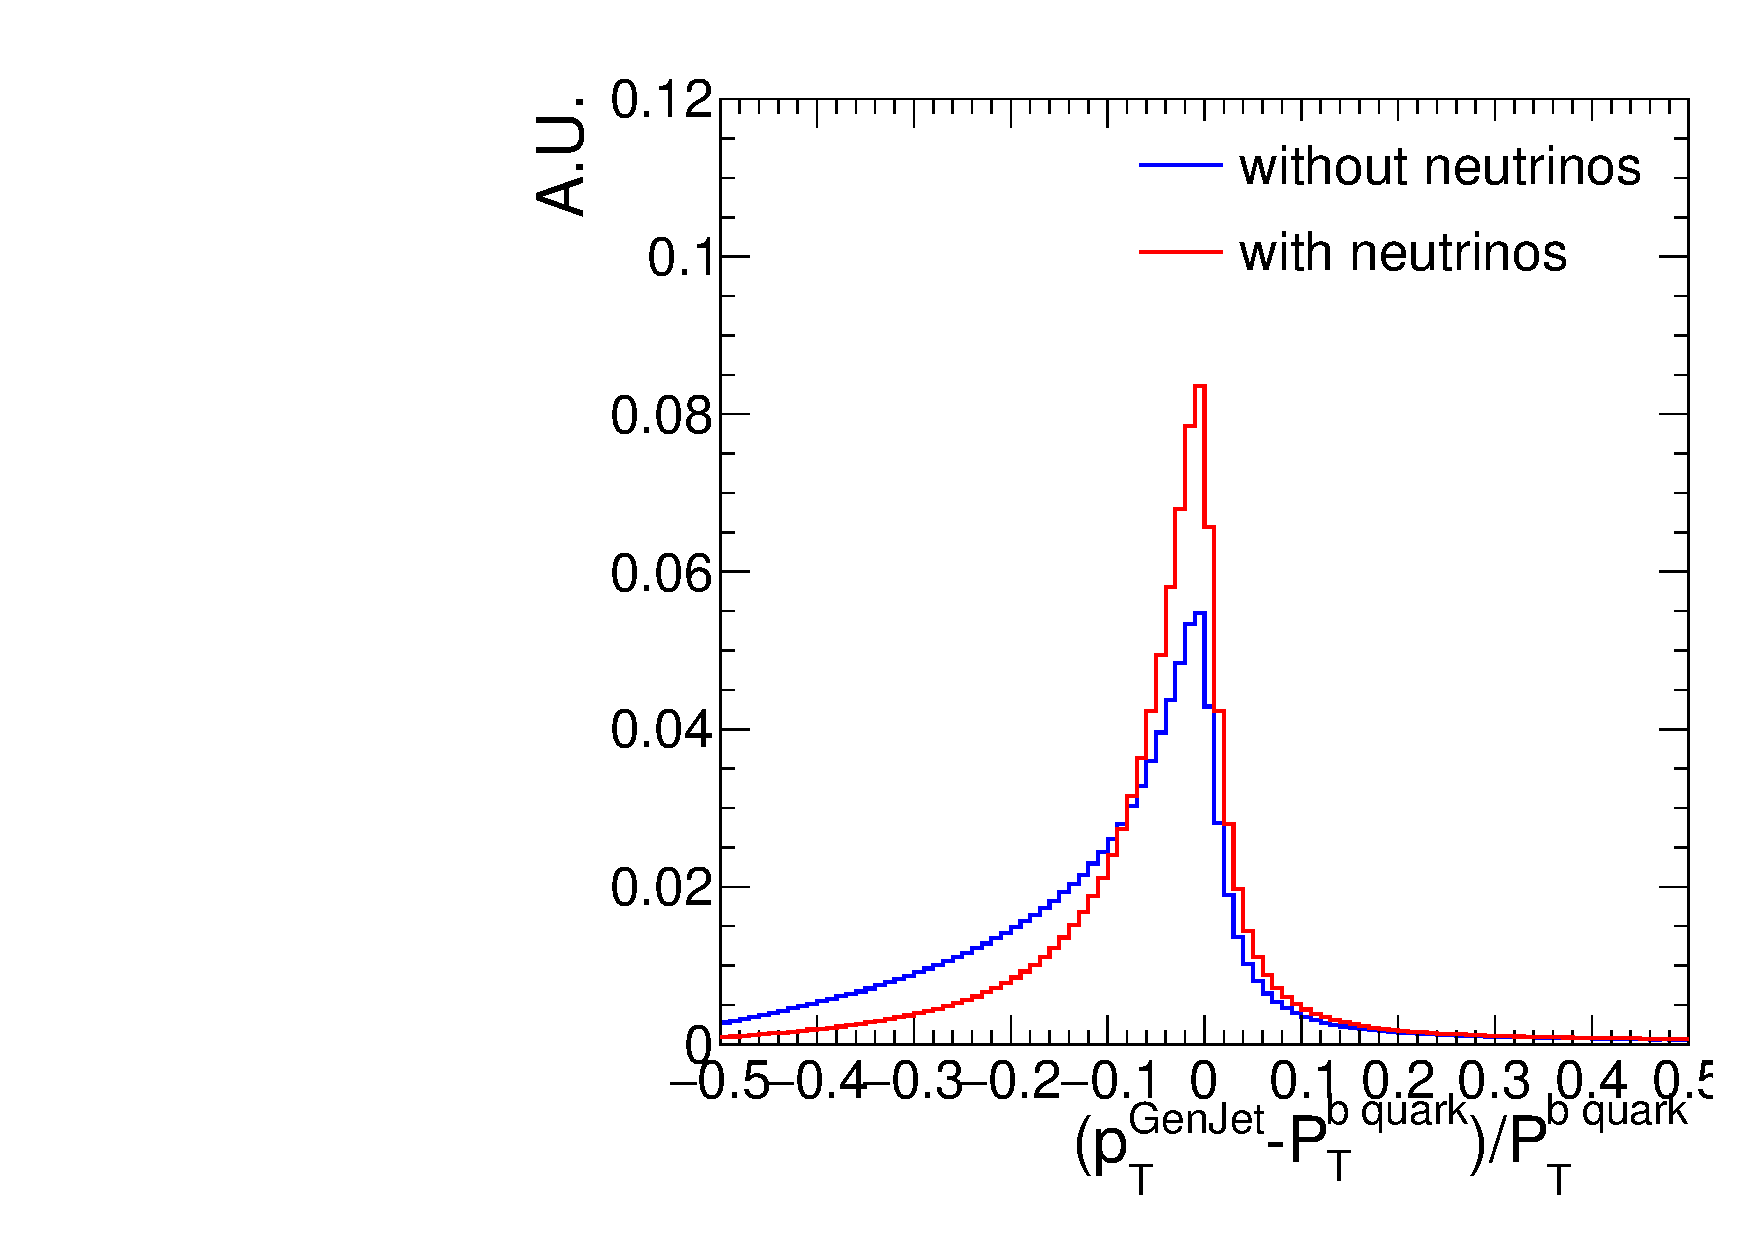
\includegraphics[width=0.33\textwidth]{b-reg/input_noBins_GenJetPtGenPtRel}\hfil
  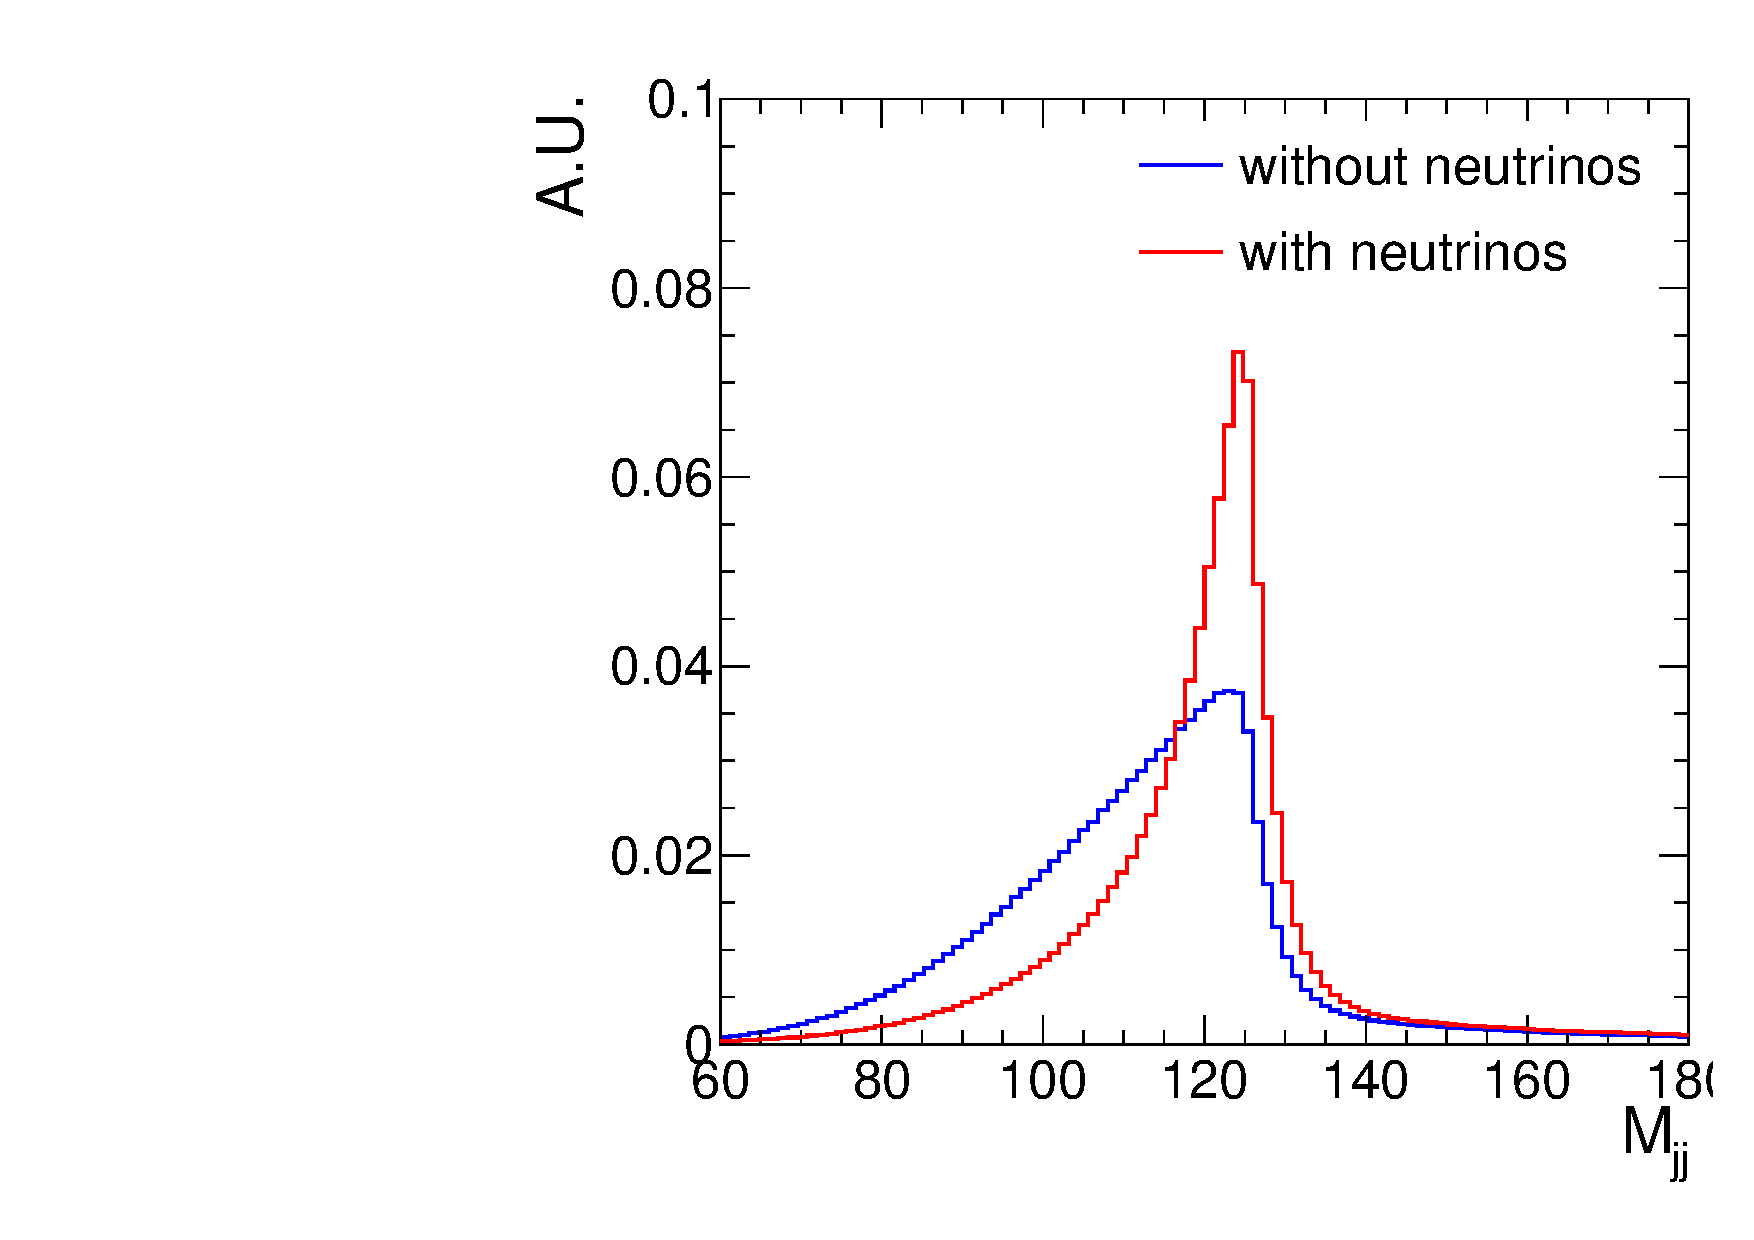
\includegraphics[width=0.33\textwidth]{b-reg/input_noBins_jjMass_Jetgenjet}\hfil
  \includegraphics[width=0.33\textwidth]{b-reg/input_noBins_jjjjMass_Jetgenjet}\hfil

  \caption{Relative \PT difference, $m_{jj}$ and $m_{jjjj}$ distributions of the b-quark and the
    corresponding gen-jet, obtained from $\HH\to\bbbb$ samples. Red
    histogram is for gen-jets containing neutrinos, blue is for jets
    without neutrinos.}
  \label{fig:b-reg-quark}
\end{figure*}

For the training we select jets that satisfy the following criteria:
\begin{itemize}
\item $\PT > 20\GeV$, $|\eta| < 2.4$
\item Matched to the generated level jet within a cone $\DR<0.4$ (this matching is done as part of MiniAOD reconstruction)
\item Matched to a b-quark within a cone $\DR<0.4$
\end{itemize}


We perform six different trainings to check the impact of additional variables:
\begin{itemize}
\item Using 15 variables based on $\Hbb$ training, listed in
  Table~\ref{tab:reg-vars}. It is denoted as \textbf{Baseline} on the
  figures below.
\item Using 15 variables plus \MET and $\Delta\phi(Jet, \MET)$.
\item Using 15 variables plus \MET , $\Delta\phi(Jet, \MET)$, and also
  $\Delta R$(Leading jet, Trailing jet).  This training is denoted as
  \textbf{full 15+3var} in the text.
\item Using 15 variables as above but in addition, for each pair of
  jets from the Higgs boson, the training is performed separately for
  the leading and trailing jets. That is, two XML weight files are
  derived, one for the leading and one for the trailing jet in the
  event.  This method is denoted as \textbf{js} on the figures and in
  the text.
\item Using 15 plus \MET and $\Delta\phi(Jet, \MET)$ variables, and
  separating the training for leading and trailing jets as above.
\item Using 15 plus \MET, $\Delta\phi(Jet, \MET)$ and $\Delta R$
  variables, and separating the training for leading and trailing jets
  as above.
\end{itemize}

The regression is performed with the TMVA package, using the Boosted Decision Tree technique with gradient boosting. 500 decision trees with depth 5 are created to estimate the target. 
The pruning technique is applied.
The detailed TMVA modified options are as follows:

\verb|NTrees=500:MaxDepth=5:nCuts=500:BoostType=Grad:!UseBaggedGrad|

\verb|Shrinkage=0.1:MinNodeSize=1:PruneStrength=5:PruneMethod=CostComplexity|

\verb|NegWeightTreatment=IgnoreNegWeightsInTraining|

After the training is done, its performance is checked in signal samples, $X\to\HH\to\ggbb$, at all mass points of $m_X$.  
The selection is the same as the training samples. 
All of our trainings are compared with the one done by $\Hbb$ analysis, which is denoted as \textbf{Hbb} on the figures. 
The $\PT^{reco}$ of the reconstructed jet can be compared to the target $\PT^{gen}$ of the generated jet with neutrinos. 
An example of such distributions is shown in Fig.~\ref{fig:b-reg-pt-res} for the leading and trailing jets. 
From distributions such as in Fig.~\ref{fig:b-reg-pt-res} we obtain the mean value for the \textbf{scale} and sigma ($\sigma$) for the \textbf{resolution}. 
The mean value and sigma are obtained from the Bukin function fit. 
The scale and resolution of the leading and trailing jets versus their \PT are shown in Fig.~\ref{fig:b-reg-jet-res}. 
From this figure we can conclude that adding MET variables into the training improves significantly the resolution. 
As expected the \textbf{15+3var js} training gives best per-jet resolution across the whole \PT range.

\begin{figure*}[h]
  \centering
  \includegraphics[width=0.35\textwidth]{b-reg/AN_mass300_J1}\hfil
  \includegraphics[width=0.35\textwidth]{b-reg/AN_mass300_J2}\hfil
  \caption{Relative \PT difference of the reconstructed and generated
    level jets after regression (red histograms) and without
    the regression (blue histograms).}
  \label{fig:b-reg-pt-res}
\end{figure*}

\begin{figure*}[h]
  \centering
  \includegraphics[width=0.35\textwidth]{b-reg/AN_HHbbgg_G_sigma_jet1pT}\hfil
  \includegraphics[width=0.35\textwidth]{b-reg/AN_HHbbgg_G_sigma_jet2pT}\hfil\\
  \caption{The resolution of the jet \PT for leading (left) and trailing (right) jets from the signal
    sample $G\to\HH\to\ggbb$.}
  \label{fig:b-reg-jet-res}
\end{figure*}
  
  \begin{figure*}[h]
  \centering
  \includegraphics[width=0.35\textwidth]{b-reg/AN_HHbbgg_G_scale_jet1pT}\hfil
  \includegraphics[width=0.35\textwidth]{b-reg/AN_HHbbgg_G_scale_jet2pT}\hfil\\
  \caption{The scale of the jet \PT for leading (left) and trailing (right) jets from the signal
    sample $G\to\HH\to\ggbb$.}
  \label{fig:b-reg-jet-scale}
\end{figure*}

The purpose of the regression is to improve the Higgs boson mass resolution from the $\Hbb$ decay in $X\to\HH\to\ggbb$ signal.  
The distributions together with the fit by Bukin function are shown in Figs.~\ref{fig:b-reg-mH-fit-reco}, where the reconstructed mass is shown after the \textbf{full 15+3var js} regression training, for $m_G = 300\GeV$ and $m_G = 900\GeV$.

After the fitting to the corresponding function is done, we obtain the mean and the width parameters of the fit.  
The width and mean (both in \GeV) are shown on Fig.~\ref{fig:b-reg-mH-res} versus the mass of the Graviton particle.  
From this figure we arrive at the same conclusion  as for single-jet plots of Fig.~\ref{fig:b-reg-jet-res}: the MET variables improve the resolution and the \textbf{full 15+3var js} training gives the best mass resolution. 
The training with \textbf{15} variables give similar results to the \textbf{Hbb} training.  
In all trainings the scale does not match the nominal value of the Higgs boson mass. 
This is expected because the jets (both at reco and gen levels) do not contain the whole energy of the Higgs boson decay.

\begin{figure*}[h]
  \centering
  \includegraphics[width=0.35\textwidth]{b-reg/AN_mass300}\hfil
  \includegraphics[width=0.35\textwidth]{b-reg/AN_mass900}\hfil
  \caption{$M_{jj}$ distributions from the reco-jets before and after
    the \textbf{full variables with js} regression for $m_G=300\GeV$ signal sample
    (left) and $m_G=900\GeV$ signal sample (right).}
  \label{fig:b-reg-mH-fit-reco}
\end{figure*}

\begin{figure*}[h]
  \centering
  \includegraphics[width=0.35\textwidth]{b-reg/AN_HHbbgg_G_sigma_Mass}\hfil
  \includegraphics[width=0.35\textwidth]{b-reg/AN_HHbbgg_G_scale_Mass}\hfil
  \caption{Performance plot comparing different regression trainings.}
  \label{fig:b-reg-mH-res}
\end{figure*}


In order to validate the developed regression in data we select events with $\Z\to\ell\ell$ decay which also contain two b-tagged jets. 
It is assumed that a di-jet is recoiled against $\Z$ boson, and therefore the $\PT(jj)$ must balance the $\PT(\ell\ell)$.  
This check was done both in muon and electron channels of \Z boson decay, analyzing \verb|DoubleMuon| and \verb|DoubleElectron| datasets correspondingly, using 2016 data.

In the muon channel the events were selected with an OR of two triggers:
\begin{itemize}
\item \verb|HLT_Mu17_TrkIsoVVL_Mu8_TrkIsoVVL_DZ| and 
\item \verb|HLT_Mu17_TrkIsoVVL_TkMu8_TrkIsoVVL_DZ|. 
\end{itemize}
The reconstructed muons must pass Tight muon ID and Loose PF isolation. 

In the electron channel the \verb|HLT_Ele23_Ele12_CaloIdL_TrackIdL_IsoVL_DZ| trigger was used and
the electrons required to pass MVA ID WP90 selection.  
Further event selection requirements in both channels are: $\PT(\ell_1) > 25\GeV$,
$\PT(\ell_2) > 15\GeV$, $\PT(\ell\ell) > 50\GeV$,
$75<m_{\ell\ell}<105\GeV$, $\Delta R^{min}_{\ell, jet} > 0.4$. The two
jets in the event must pass Loose PF ID selection, Medium PU jet ID,
tagged as b-jets with CSVv2 Medium WP, and have $\PT>20\GeV$,
$|\eta|<2.4$.

\begin{figure*}[thb]
  \centering
  \includegraphics[width=0.32\textwidth]{b-reg/Vali_Data_MC_no_reg__PtBalance_mu_Medium}\hfil
  \includegraphics[width=0.32\textwidth]{b-reg/Vali_Data_MC_jet_15plus3_js_2_27__PtBalance_mu_Medium}\hfil
  \includegraphics[width=0.32\textwidth]{b-reg/Vali_Data_MC_jet_Hbb__PtBalance_mu_Medium}\hfil\\
  \includegraphics[width=0.32\textwidth]{b-reg/Vali_Data_MC_no_reg__PtBalance_ele_Medium}\hfil
  \includegraphics[width=0.32\textwidth]{b-reg/Vali_Data_MC_jet_15plus3_js_2_27__PtBalance_ele_Medium}\hfil
  \includegraphics[width=0.32\textwidth]{b-reg/Vali_Data_MC_jet_Hbb__PtBalance_ele_Medium}\hfil\\
  \includegraphics[width=0.32\textwidth]{b-reg/Vali_Data_MC_no_reg__PtBalance_all_Medium}\hfil
  \includegraphics[width=0.32\textwidth]{b-reg/Vali_Data_MC_jet_15plus3_js_2_27__PtBalance_all_Medium}\hfil
  \includegraphics[width=0.32\textwidth]{b-reg/Vali_Data_MC_jet_Hbb__PtBalance_ele_Medium}\hfil\\
  \caption{Pt balance (ratio) of the di-jet and di-lepton. On the left
    are the distributions without regression, in the center - using
    \textbf{full 15+3var js} training and on the right - using
    \textbf{Hbb} regression.  Top plots are for muon channel, middle
    for electron channel and bottom is the combination (sum) of the
    two.}
  \label{fig:vali-pt}
\end{figure*}

Figure \ref{fig:vali-pt} shows the mentioned $\PT$-balance
distributions, $\PT^{jj}/\PT^{\ell\ell}$.  The data is compared to the
MC predictions. It can be seen that before any regression is applied to avoid over training.
(left plots) the peak of the ratio distribution is below one. With the
regression applied the peak moves to 1 for both our \textbf{full variables with js}
 training (center) and the one from \textbf{Hbb} (right). The
trend is the same in data and MC.  This indicates that the regression
does indeed brings the $\PT$ of the $b$-jets closer to their true
values.

Similarly, figure~\ref{fig:vali-Mjj} shows the mass distributions,
$m_{jj}$, before and after regression. These figures indicate that
$m_{jj}$ is not distorted in any bad way, no artificial peaks are
created. This ensures us that the background distributions in our
analysis signal region will not be distorted either.


\begin{figure*}[thb]
  \centering
  \includegraphics[width=0.32\textwidth]{b-reg/Vali_Data_MC_no_reg__Mjj_mu_Medium}\hfil
  \includegraphics[width=0.32\textwidth]{b-reg/Vali_Data_MC_jet_15plus3_js_2_27__Mjj_mu_Medium}\hfil
  \includegraphics[width=0.32\textwidth]{b-reg/Vali_Data_MC_jet_Hbb__Mjj_mu_Medium}\hfil\\
  \includegraphics[width=0.32\textwidth]{b-reg/Vali_Data_MC_no_reg__Mjj_ele_Medium}\hfil
  \includegraphics[width=0.32\textwidth]{b-reg/Vali_Data_MC_jet_15plus3_js_2_27__Mjj_ele_Medium}\hfil
  \includegraphics[width=0.32\textwidth]{b-reg/Vali_Data_MC_jet_Hbb__Mjj_ele_Medium}\hfil\\
  \includegraphics[width=0.32\textwidth]{b-reg/Vali_Data_MC_no_reg__Mjj_all_Medium}\hfil
  \includegraphics[width=0.32\textwidth]{b-reg/Vali_Data_MC_jet_15plus3_js_2_27__Mjj_all_Medium}\hfil
  \includegraphics[width=0.32\textwidth]{b-reg/Vali_Data_MC_jet_Hbb__Mjj_all_Medium}\hfil\\
  \caption{Distributions of the $m_{jj}$. On the left are plots with
    no regression, in the center - using \textbf{full 15+3var js}
    training and on the right - using \textbf{Hbb} regression.  Top
    plots for muon channel, middle for electron channel and bottom is
    the combination (sum) of the two.  }
  \label{fig:vali-Mjj}
\end{figure*}

\clearpage

\subsubsection{B-tagging}
\label{sec:btag}

We utilize the \textit{Combined Secondary Vertex} algorithm (CSVv2) for tagging b-jets,
described in Ref.~\cite{btag-twiki}. This b-tagging score for leading and subleading jets is then used in the MVA categorization.

The b-tagging scale factors have been calculated according to the BTV recipe, including the in situ calculation of signal efficiency.
The signal efficiency has been calculated for all signal samples combined, in bins of $p_{T}$ and $|\eta|$.
The efficiency plots for tight WP, medium WP and loose WP can be seen in figure \ref{fig:btageff}.

\begin{figure*}[h]
  \centering
  \includegraphics[width=0.45\textwidth]{figures/sec-jets/btageff_tight.pdf}\hfil
  \includegraphics[width=0.45\textwidth]{figures/sec-jets/btageff_medium.pdf}\hfil
  \includegraphics[width=0.45\textwidth]{figures/sec-jets/btageff_loose.pdf}\hfil 
  \caption{B-tagging efficiency for tight, medium and loose working points, as a function of jet $p_{T}$ and $|\eta|$.}
  \label{fig:btageff}
\end{figure*}


\section{MVA Based Categorization}
\label{sec:cats}

During the analysis, it has been noticed that different kinematic variables could potentially contribute to constraining the background contribution in the signal region without cutting too much on the signal efficiency. 
However, this large-dimensional optimization procedure (all investigated variables) was not optimal. 
Instead, we have developed a multivariate analysis (MVA), combining these different variables, into a single discriminant. 
This discriminant is used to categorize the events in High Purity, Medium Purity categories and a control region, similarly to the cut based categorization. 

The input variables investigated for this MVA were:
\begin{itemize}
\item Leading and subleading jets b-tagging score;
\item Helicity angles $|cos(\theta^{*}_{CS})|$, $|cos(\theta^{*}_{bb})|$ and $|cos(\theta^{*}_{\gamma\gamma})|$: $|cos(\theta^{*}_{CS})|$ is defined as the angle between the direction of the $H\rightarrow\gamma\gamma$ candidate to the Colin-Sopper reference frame (assumes each incoming particle in the scattering to have 6.5 TeV); $|cos(\theta^{*}_{xx})|$ is defined as the angle between the particle $x$ and the direction defined by the $H\rightarrow x x$ candidate (randomly choosing between x's), where $x = \gamma$ or $b$;
\item $p_{T}(\gamma\gamma)/M(jj\gamma\gamma)$ and $p_{T}(jj)/M(jj\gamma\gamma)$
\end{itemize}

The training was performed in the photon control region, as described in \ref{sec:PCR}. 
Plots comparing the input variables in the photon control region and the blinded signal region are shown in Figure \ref{fig:inputmva}. 
As our signal in the training, we sum the 14 non-resonant HH samples available (box only, SM, and 12 BSM points). 
Thus, we have a training that is not specific to a single region in the parameter space, maintaining the sensitivities comparable between the benchmark points (as it is with the cut based categorization). 

\begin{figure*}[h]
  \centering
  \includegraphics[width=0.3\textwidth]{figures/sec-cats/mva/ljbdis}\hfil
  \includegraphics[width=0.3\textwidth]{figures/sec-cats/mva/sjbdis}\hfil
  \includegraphics[width=0.3\textwidth]{figures/sec-cats/mva/cts_cs}\hfil
  \includegraphics[width=0.3\textwidth]{figures/sec-cats/mva/ct_bb}\hfil
  \includegraphics[width=0.3\textwidth]{figures/sec-cats/mva/ct_gg}\hfil
  \includegraphics[width=0.3\textwidth]{figures/sec-cats/mva/gghhr}\hfil
  \includegraphics[width=0.3\textwidth]{figures/sec-cats/mva/bbhhr}\hfil
  \caption{Distributions of input variables in the blinded photon control region, blinded signal region, and SM HH sample. All normalized to unity. }
  \label{fig:inputmva}
\end{figure*}

To improve the training, we split the training into two regions: low mass and high mass. 
The low mass training is performed with events with $\tilde{M}_{X}$ below 350 GeV, while the high mass training uses the complementary region. 
The training is based on a decision tree boosted with the gradient algorithm, with the trees randomized between iterations to decrease overtraining. 
To implement the training the TMVA package was used. 
%The TMVA output plots are shown for both trainings in Figures \ref{fig:mva_hm} and \ref{fig:mva_lm}. 
From now on, we will refer to the training discriminant variable as HHTagger.

With the HHTagger discriminant, we build our two signal categories based on the optimization of the expected SM HH limit, separately in the high mass and in the low mass regions. 
These categories are called high purity category (HPC) and medium purity category (MPC); their names refer to their signal and background content. 
As signal, we use the SM HH sample to calculate the sensitivity. 
The outcome of this study was the categorization in Table \ref{tab:catmva}. 
The expected number of background events, when comparing MPC and HPC between cut based and MVA approaches, is comparable and consistent, while for the number of signal events, the performance is better for the HHTagger categorization. 

We also have to ensure that the HHTagger selection does not distort our variables of interest, $\Mjj$ and $\Mgg$. 
We demonstrate that there is no appreciable shaping by comparing the $\Mjj$ and $\Mgg$ shapes in different bins of the HHTagger discriminant. 
This can be seen in Figure \ref{fig:mva_mggmjj}. 

\begin{table}
\centering
    \begin{tabular}{| c | c | c |}
    \hline
    Mass Region & HPC & MPC \\ \hline
    Low Mass & HHTagger $> 0.96$ & $ 0.75 < $ HHTagger $ < 0.96 $ \\ \hline 
    High Mass & HHTagger $> 0.96$ & $ 0.6 < $ HHTagger $ < 0.96 $ \\ \hline 
    \end{tabular}
\caption{Non-resonant categorization with HHTagger discriminant.}
\label{tab:catmva}
\end{table}


%\begin{figure*}[h]
%  \centering
%  \includegraphics[width=0.45\textwidth]{figures/sec-cats/mva/vars1_hm400}\hfil
%  \includegraphics[width=0.45\textwidth]{figures/sec-cats/mva/vars2_hm400}\hfil
%  \includegraphics[width=0.45\textwidth]{figures/sec-cats/mva/corsS_hm400}\hfil
%  \includegraphics[width=0.45\textwidth]{figures/sec-cats/mva/corsB_hm400}\hfil
%  \includegraphics[width=0.45\textwidth]{figures/sec-cats/mva/ROC_hm400}\hfil
%  \includegraphics[width=0.45\textwidth]{figures/sec-cats/mva/discr_hm400}\hfil
%  \caption{TMVA output plots for the High Mass Training.}
%  \label{fig:mva_hm}
%\end{figure*}

%\begin{figure*}[h]
%  \centering
%  \includegraphics[width=0.45\textwidth]{figures/sec-cats/mva/vars1_lm400}\hfil
%  \includegraphics[width=0.45\textwidth]{figures/sec-cats/mva/vars2_lm400}\hfil
%  \includegraphics[width=0.45\textwidth]{figures/sec-cats/mva/corsS_lm400}\hfil
%  \includegraphics[width=0.45\textwidth]{figures/sec-cats/mva/corsB_lm400}\hfil
%  \includegraphics[width=0.45\textwidth]{figures/sec-cats/mva/ROC_lm400}\hfil
%  \includegraphics[width=0.45\textwidth]{figures/sec-cats/mva/discr_lm400}\hfil
%  \caption{TMVA output plots for the Low Mass Training.}
%  \label{fig:mva_lm}
%\end{figure*}

\begin{figure*}[h]
  \centering
  \includegraphics[width=0.45\textwidth]{figures/sec-cats/mva/hhtag_mgg}\hfil
  \includegraphics[width=0.45\textwidth]{figures/sec-cats/mva/hhtag_mjj}\hfil
  \caption{Photon control region distributions of $\Mgg$ (left) and $\Mjj$ (right) in bins of HHTagger. Although the slope changes between bins, this effect does not influence the limit setting.}
  \label{fig:mva_mggmjj}
\end{figure*}

\subsubsection{Performance Cross-Checks}

We have performed several cross checks to look for possible improvements on the MVA categorization. 

\begin{itemize}
\item \textbf{Signal Hypothesis}
\end{itemize}

In the standard training, the sum of all non-resonant samples are used as the signal hypothesis. 
However, this might not be the optimal training for the SM HH case. 
To test this, we compare the performance of different trainings assuming the SM HH signal. 
The signal hypotheses tested are:
\begin{itemize}
\item All non-resonant (standard);
\item SM HH;
\item SM HH, with separate training for the high mass and low mass region (similar to standard);
\item SM HH + Node 3 (this node, as defined in Table \ref{tab:bench_old}, contains the SM point);
\item SM HH + Node 3, with separate training for the high mass and low mass region (similar to standard).
\end{itemize}
The background hypothesis for this test is the photon control region, in the high mass region. 

\begin{figure*}[h]
  \centering
  \includegraphics[width=0.7\textwidth]{figures/sec-cats/mva/ROC}\hfil
  \caption{ROC curves with different signal hypotheses for training. The performance is evaluated in the high mass region, with the photon control region as background and SM HH as signal.}
  \label{fig:mva_cc_signal}
\end{figure*}


The ROC curves from the different trainings are shown in Figure \ref{fig:mva_cc_signal}. 
Since no significant improvement is seen in the high purity region (for background rejection larger than 95\%, a typical value for the chosen WPs), the standard training method is kept in use. 

\begin{itemize}
\item \textbf{Background Hypothesis}
\end{itemize}

In the standard training, the photon control region is used as a background model, avoiding MC reliance. 
However, this might not be optimal because the photon control region might have different correlations between the MVA variables with respect to the signal region. 
To test this, we compare the performance of different trainings assuming different background hypotheses: 
\begin{itemize}
\item Photon control region (standard);
\item Blinded signal region;
\item Blinded control region (to ensure that the difference between the two previous trainings does not come from blinding).
\end{itemize}
The background hypothesis for this test is the blinded signal region, in the high mass region, and the signal hypothesis is SM HH. 

\begin{figure*}[h]
  \centering
  \includegraphics[width=0.7\textwidth]{figures/sec-cats/mva/ROC_BCR}\hfil
  \caption{ROC curves with different background hypotheses for training. The performance is evaluated in the high mass region, with the blinded signal region as background and SM HH as signal.}
  \label{fig:mva_cc_background}
\end{figure*}

The ROC curves from the different trainings are shown in Figure \ref{fig:mva_cc_background}. 
While some improvement is seen, this training is not optimal for statistical reasons. 
The blinded signal region contains significantly less events than the photon control region. 
This limits the precision and accuracy of the multivariate analysis training. 
Specifically, it has been observed that the blinded signal region does not contain events in the high BDT region (signal-like phase space), which can cause over training. 
The second issue is that, optimally, training on a dataset that is statistically independent from the one to which it will be applied leads to a more robust procedure. 



\begin{itemize}
\item \textbf{Resonant Hypothesis}
\end{itemize}

\begin{figure*}[h]
  \centering
  \includegraphics[width=0.7\textwidth]{figures/sec-cats/mva/ROC_res}\hfil
  \caption{ROC curves with different signal hypotheses for training. The performance is evaluated in the low mass region, with the photon control region as background and the 300 GeV radion sample as signal.}
  \label{fig:mva_cc_res}
\end{figure*}

While this MVA is trained with the non-resonant signal hypotheses, it can also be applied to the resonant search. 
We check, however, if a dedicated training with the resonant samples as signal hypothesis performs better, when applying the categorization to the resonant analysis.  
This is tested by comparing the categorization performance of the standard training versus a resonant training on a resonant signal point. 
The plot in Figure \ref{fig:mva_cc_res}, these two trainings are shown and no significant difference is seen. 
Therefore the standard, non-resonant training will be used also for the resonant analysis. 





\section{ $\Mtilde$ and Mass Window Selection}
\label{sec:masswindow}

In order to increase the sensitivity of the resonant analysis, we perform a cut on the 4-body invariant mass before the signal extraction with the 2D fit.
In the Run I analysis, the 4-body invariant mass was corrected with a kinematic fit, to mitigate the effects of the low mass resolution of the dijet system.
However, it has been seen that this method is too reliant on the a-priori set of energy and spatial resolutions for the jets in that analysis (these resolutions must be measured in situ, since they are kinematic dependent).
One solution for this was to use instead the variable $\Mtilde$, defined as:

\begin{equation}
\Mtilde = \Mjjgg - \Mjj - \Mgg + 250 \text{ GeV}.
\end{equation}

This variable performs a kinematic fit "by hand", by effectively scaling the dijet and diphoton invariant masses to 125 GeV. 
In order to quantify the improvementof this variable with respect to other 4-body invariant mass reconstructions, we calculate the width of the smallest interval that covers $68\%$ of the signal shape in each reconstruction method. 
We compare $\Mtilde$ with the standard $\Mjjgg$ and with $\Mjjgg_{KF}$, which is reconstructed with a kinematic fit in $\Mjj$, which tries to vary the jets within their uncertainties to achieve $\Mjj = 125$ GeV. 
The widths are compared in Figure \ref{fig:mxwidth}. 

\begin{figure*}[thb]
  \centering
  \includegraphics[width=0.6\textwidth]{figures/sec-window/width_67_prime.pdf}\hfil
  \caption{Different 4-body mass widths: $\Mtilde$, $\Mjjgg$ with kinematic fit, and $\Mjjgg$ with no extra corrections.}
  \label{fig:mxwidth}
\end{figure*}

The effect of reconstructing the 4-body invariant mass with $\Mtilde$ on the signal shape can be seen in \ref{fig:mx}. 
The figure shows that the $\Mtilde$ reconstruction yields a better performing resolution for the 4-body invariant mass reconstruction, meaning that we can perform tighter cuts on it and increase the signal/background for each signal mass point.

One extra check we must do while using this variable is to make sure there are no unexpected effects on the background shapes. 
The effect of $\Mtilde$ is similar to the kinematic fitted $\Mjjgg$, but more pronounced, which is the sharp kinematic cut around the $\Mtilde = 250$ GeV point. This can be seen in the figures in section \ref{sec:control}..

\begin{figure*}[thb]
  \centering
  \includegraphics[width=0.6\textwidth]{figures/sec-window/prplot.pdf}\hfil
  \caption{Different 4-body mass reconstructions: $\Mtilde$ (dotted line), $\Mjjgg$ with kinematic fit (dashed line), and $\Mjjgg$ with no extra correction (full line). Signals for different radion masses are shown. The normalizations are such that the non-corrected mass peaks at 1 (same normalization for different reconstructions in each mass point). This plot is made after full selection, in the b-tagging signal region (at least one medium b-tagged jet).}
  \label{fig:mx}
\end{figure*}

It has also been observed that, for the non-resonant signal samples, the $\Mtilde$ variable approaches the generator level HH invariant mass distribution more so than the kinematic fitted $\Mjjgg$ and the default 4-body invariant mass. This can be seen in figure \ref{fig:mxnonres}. For this, $\Mtilde$ will also be used in the non-resonant analysis.

\begin{figure*}[thb]
  \centering
  \includegraphics[width=0.45\textwidth]{figures/sec-window/nonresmx.pdf}\hfil
  \caption{Behavior of $\Mtilde$, $\Mggjj$ and GEN-level $M(hh)$. WARNING - THIS IS THE 2015 PLOT}
  \label{fig:mxnonres}
\end{figure*}

One desirable effect of the $\Mtilde$ definition in this version of the analysis, compared to the 2015 definition (which only scaled the $\Mjj$ value as in $\Mtilde = \Mjjgg - \Mjj + 125$ GeV), is that a $\Mtilde$ selection does not bias $\Mgg$ and $\Mjj$. 
This can be seen in the 2D plots of $\Mtilde:\Mgg$ and $\Mtilde:\Mjj$ in Figure \ref{fog:mx2d}. 

\begin{figure*}[thb]
  \centering
  \includegraphics[width=0.45\textwidth]{figures/sec-window/mgg2d.pdf}\hfil
  \includegraphics[width=0.45\textwidth]{figures/sec-window/mjj2d.pdf}\hfil
  \caption{$\Mtilde:\Mgg$ and $\Mtilde:\Mjj$ in the photon control region, scaled to unity and Z-axis in log scale. }
  \label{fig:mx2d}
\end{figure*}

With $\Mtilde$, we can improve the resonant analysis by tightening the signal region around the 4-body resonance mass (mass window). 
Through limits optimization, it has been checked that constructing a mass window with the smallest interval that covers $60\%$ of the signal shape provides the best sensitivity. 
The size of these intervals, as a function of the hypothesis mass, is seen in Figure \ref{fig:masswindowwidths}. 

\begin{figure*}[thb]
  \centering
  \includegraphics[width=0.45\textwidth]{figures/sec-window/width_60_prime.pdf}\hfil

  \caption{Mass window sizes as a function of the resonance mass. }
  \label{fig:masswindowwidths}
\end{figure*}

We implement this mass window by requiring that $W_{-} < \Mtilde < W_{+}$. 
$W_{\pm}$ are calculated based on the widths defined in Figure \ref{fig:masswindowwidths}. 
We fit $W_{\pm}$ with a 3rd degree polynomial so that the mass windows can be defined functionally based on the mass hypothesis. 
These fits, and, therefore, the definition of $W_{\pm}$ can be seen in Figure \ref{fig:masswindowfit}. 
$W_{\pm}$ can be infered through the Y-axis of \ref{fig:masswindowfit}, $W_{-}$ is defined by the blue curve and $W_{+}$ by the red. 

\begin{figure*}[thb]
  \centering
  \includegraphics[width=0.45\textwidth]{figures/sec-window/fit_60_prime.pdf}\hfil

  \caption{Mass window sizes as a function of the resonance mass. }
  \label{fig:masswindowfit}
\end{figure*}


\section{Selection Efficiencies}
\label{sec:selection}

As a summary of the previous sections, the cut flow of the analysis is as follows:
\begin{itemize}
\item At least two photons and two jets in the event
\item At least two photons pass the trigger based pre-selection (see sec. \ref{sec:trigger});
\item At least two photons pass the kinematic and identification requirements (see sec. \ref{sec:photons}) $\to$ select two highest $E_{T}$ photons as diphoton candidate;
\item At least two jets pass the kinematic selection (see sec. \ref{sec:jets}) $\to$ select two jets with highest b-tagging score as dijet candidate;
\item Event can be classified in either High Purity Category or Medium Purity Category;
\end{itemize}

The efficiency after each step above and taking into account the acceptance is estimated and shown for each of the signal samples considered in our analysis. 
In Figure \ref{fig:cutflow-res}, the signal efficiency for Radions (spin-0) and Gravitons (spin-2) from mass hypothesis of 250 up to 900 GeV. 
In Figure \ref{fig:cutflow-nonres}, the signal efficiency for the non-resonant nodes, including top-only contribution (Node 0) and SM (Node 1). 

%We also performed the selection using the cut based photon identification. The ratio of the efficiencies is performed to assess the performance difference between the different photon Id. The result of the comparison is shown in top figure~\ref{fig:cutflow-signal-diff-CutB} and bottom figure~\ref{fig:cutflow-signal-diff-CutB} for Graviton and Radion samples, respectively. The performance of the EGamma MVA photon identification outrates the one of the cut based photon Id., by 10. to 15. \% at low resonance masses, and is around 8-10\% for high resonance masses. \\
%Although we performed a detail study of the MVA photon id. and shown that we could choose a different WP from EGamma MVA(see table~\ref{tab:MVA-WP}), the efficiency for the latter is expectedly  better as shown in figure~\ref{fig:cutflow-signal-diff-MVAEG}.\\
%A comparison of the Graviton and Radion signal efficiencies is also performed in figure~\ref{fig:cutflow-signal-diff-RG}. It is shown that Graviton samples show a better efficiency, more than 10\% higher for high masses.

\begin{figure*}[h]
  \centering
  \includegraphics[width=0.45\textwidth]{figures/sec-efficiency_plots/wRegression/res_effs_Graviton_reg.pdf}\hfil
  \includegraphics[width=0.45\textwidth]{figures/sec-efficiency_plots/wRegression/res_effs_Radion_reg.pdf}\hfil
  \caption{Graviton (left) and Radion (right) signal acceptance$\times$efficiency for each cut (described in text).}
  \label{fig:cutflow-res}
\end{figure*}

\begin{figure*}[h]
  \centering
  \includegraphics[width=0.45\textwidth]{figures/sec-efficiency_plots/wRegression/nonres_effs_reg.pdf}\hfil
  \caption{Non-resonant acceptance x efficiency. Jet energy regression applied in addition to MVA based categorization.}
  \label{fig:cutflow-nonres}
\end{figure*}



\section{Control Plots}
\label{sec:control}

To validate the Monte Carlo simulations, we produce data/Monte Carlo comparison plots (control plots) of the signal region (SR), blinded in the $115 < \Mgg < 130$ GeV region.  
For background and data to match, the DiPhoton+Jets contribution has been scaled by a factor of 1.5, while the prompt-fake and fake-fake contributions from the GJets and QCD samples have been scaled to data. 
The signal in these plots is normalized for $500$ fb.

It's a well known fact that modeling backgrounds with fake objects, such as jets identified as photons, leads to discrepancies when using MC simulation. 
This is one of the reasons why all background modeling performed in this analysis, both during limit extraction and MVA training, is done with data driven methods. 
The plots shown in this section aim to show that we understand the composition of the background, which is basically equally split between the contribution with two "real" photons, and the contribution with one "real" photon and one jet identified as a photon.


\begin{figure*}[thb]
  \centering
\includegraphics[width=0.45\textwidth]{figures/sec-control/NP_MXprime.pdf}\hfil
\includegraphics[width=0.45\textwidth]{figures/sec-control/NP_dicandidate_Mass.pdf}\hfil
\includegraphics[width=0.45\textwidth]{figures/sec-control/NP_diPho_Mass.pdf}\hfil
\includegraphics[width=0.45\textwidth]{figures/sec-control/NP_diJet_Mass.pdf}\hfil
\includegraphics[width=0.45\textwidth]{figures/sec-control/NP_CosThetaStar_CS.pdf}\hfil
\includegraphics[width=0.45\textwidth]{figures/sec-control/NP_CosTheta_bb.pdf}\hfil

  \caption{Distributions of data and MC for the signal region with the blinding region removed. Top left: $\Mtilde$. Top right: $\Mjjgg$. Center left: $\Mgg$. Center right: $\Mjj$. Bottom left: $|cos(\theta^{*}_{CS})|$. Bottom right: $|cos(\theta^{*}_{bb})|$.}
\label{fig:cp_mgg1}
\end{figure*}

%\begin{figure*}[thb]
%  \centering
%\includegraphics[width=0.45\textwidth]{figures/sec-control/NP_diPho_Mass.pdf}\hfil
%\includegraphics[width=0.45\textwidth]{figures/sec-control/NP_diJet_Mass.pdf}\hfil
%  \caption{Distributions of data and MC for the signal region with the blinding region removed.}
%\label{fig:cp_mgg2}
%\end{figure*}
%\begin{figure*}[thb]
%  \centering
%\includegraphics[width=0.45\textwidth]{figures/sec-control/NP_CosThetaStar_CS.pdf}\hfil
%\includegraphics[width=0.45\textwidth]{figures/sec-control/NP_CosTheta_bb.pdf}\hfil
%  \caption{Distributions of data and MC for the signal region with the blinding region removed.}
%\label{fig:cp_mgg3}
%\end{figure*}

\begin{figure*}[thb]
  \centering
\includegraphics[width=0.45\textwidth]{figures/sec-control/NP_CosTheta_gg.pdf}\hfil
\includegraphics[width=0.45\textwidth]{figures/sec-control/LOG_ggptmjjgg.pdf}\hfil
\includegraphics[width=0.45\textwidth]{figures/sec-control/LOG_jjptmjjgg.pdf}\hfil
\includegraphics[width=0.45\textwidth]{figures/sec-control/LOG_ljetptmgg}\hfil
\includegraphics[width=0.45\textwidth]{figures/sec-control/LOG_sjetptmgg}\hfil
\includegraphics[width=0.45\textwidth]{figures/sec-control/LOG_lphoptmgg}\hfil

  \caption{Distributions of data and MC for the signal region with the blinding region removed. Top left: $|cos(\theta^{*}_{\gamma\gamma})|$. Top right: $p_{T}(\gamma\gamma)/M(jj\gamma\gamma)$. Center left: $p_{T}(jj)/M(jj\gamma\gamma)$. Center right: leading jet $p_{T}(j)/\Mjj$. Bottom left: subleading jet $p_{T}(j)/\Mjj$. Bottom right: leading photon $E_{T}(\gamma)/\Mjj$}
\label{fig:cp_mgg4}
\end{figure*}

%\begin{figure*}[thb]
%  \centering
%\includegraphics[width=0.45\textwidth]{figures/sec-control/LOG_jjptmjjgg.pdf}\hfil
%\includegraphics[width=0.45\textwidth]{figures/sec-control/LOG_ljetptmgg}\hfil
%  \caption{Distributions of data and MC for the signal region with the blinding region removed.}
%\label{fig:cp_mgg5}
%\end{figure*}
%\begin{figure*}[thb]
%  \centering
%\includegraphics[width=0.45\textwidth]{figures/sec-control/LOG_sjetptmgg}\hfil
%\includegraphics[width=0.45\textwidth]{figures/sec-control/LOG_lphoptmgg}\hfil
%  \caption{Distributions of data and MC for the signal region with the blinding region removed.}
%\label{fig:cp_mgg6}
%\end{figure*}

%\begin{figure*}[thb]
%  \centering
%\includegraphics[width=0.45\textwidth]{figures/sec-control/LOG_sphoptmgg}\hfil
%  \caption{Distributions of data and MC for the signal region with the blinding region removed.}
%\label{fig:cp_mgg7}
%\end{figure*}
\begin{figure*}[thb]
  \centering
\includegraphics[width=0.65\textwidth]{figures/sec-control/NP_HHTagger_LM}
\includegraphics[width=0.65\textwidth]{figures/sec-control/NP_HHTagger_HM}
  \caption{Distributions of data and MC for the signal region with the blinding region removed. Top: Categorization MVA output (low mass training). Bottom: Categorization MVA output (high mass training).}
\label{fig:cp_mgg8}
\end{figure*}


\section{Statistical Modeling and Limit Extraction}
\label{sec:modeling}

The signal extraction and limit setting in this analysis is performed with a 2D fit in the $\Mgg:\Mjj$ plane, since we expect our signal to peak in both variables. For our background, they are expected to be uncorrelated given our statistical precision. With this last assumption, we can construct background function models as $f_{\gamma}(\Mgg)\times f_{J}(\Mjj)$, where $f_{\gamma}$ ($f_{J}$) are our functional choices to fit the diphoton (dijet) mass spectrum. A thorough explanation of the background uncorrelation hypothesis is given at the end of this section.


\subsection{Signal Model}

As a signal model in the limit extraction, we use parametric models fitted to the simulated samples after the full selection. 
Each fit is done in each different sample independently, i.e., for all resonance masses, spins and for all different non-resonant hypotheses. 
The choice of parametric model for $\Mgg$ and $\Mjj$ individually is a double-sided Crystal-Ball function. 
The double-sided Crystal-Ball function is defined as follows:
\begin{equation}
f(x;\mu, \sigma, \alpha_{L}, p_{L}, \alpha_{R}, p_{R}) = N \cdot 
\begin{cases} 
A_{L} \cdot \left( B_{L} - \frac{x - \mu}{\sigma} \right)^{-p_{L}}, & \mbox{for } \frac{x - \mu}{\sigma} > - \alpha_{L} \\
A_{R} \cdot \left( B_{R} + \frac{x - \mu}{\sigma} \right)^{-p_{R}}, & \mbox{for } \frac{x - \mu}{\sigma} > \alpha_{R} \\
e^{  \frac{\left( x - \mu \right)^{2}}{\sigma^{2}} }, & \mbox{for } \frac{x - \mu}{\sigma} < - \alpha_{L}  \mbox{ and } \frac{x - \mu}{\sigma} > \alpha_{R}
 \end{cases},
 \end{equation}
 where the $A_{L}, A_{R}, B_{L}, B_{R}$ constants are defined by:
 \begin{eqnarray}
 A_{k} &=& \left( \frac{p_{k}}{\left| \alpha_{k} \right|} \right)^{p_{k}} \cdot e^{-\frac{\alpha^{2}}{2}}, \\
 B_{k} &=& \frac{p_{k}}{\left| \alpha_{k} \right|} - \left| \alpha_{k} \right|,
 \end{eqnarray}
 where $k$ is either $L$ or $R$. This definition is such that there are two independent tails, a left tail (L) and a right tail (R), and a gaussian core.  
This signal model is enough to model both the high mass resolution of $\Mgg$ and the lower resolution of $\Mjj$. 
With respect to the signal model chosen for previous versions of the analysis, such as the 2015 analysis, this choice is beneficial when comparing to a sum of a gaussian and a single sided Crystal-Ball because the left and right tails are made completely independent, while maintaining the same number of free parameters.

These signal fits can be seen in Figures \ref{fig:rad300}, \ref{fig:rad600} and for the 300, and 600 GeV radion signals, and in figures \ref{fig:sig_highmassSM} and \ref{fig:sig_lowmassSM} the signal fits for the non-resonant SM HH production in the high mass and low mass categories, respectively.

%\begin{figure*}[h]
%  \centering
%  \includegraphics[width=0.45\textwidth]{figures/sec-signals/Rad250_signal_fit_mgg_cat0}\hfil
%  \includegraphics[width=0.45\textwidth]{figures/sec-signals/Rad250_signal_fit_mgg_cat1}\hfil
%  \includegraphics[width=0.45\textwidth]{figures/sec-signals/Rad250_signal_fit_mjj_cat0}\hfil
%  \includegraphics[width=0.45\textwidth]{figures/sec-signals/Rad250_signal_fit_mjj_cat1}\hfil
%  \caption{Signal fits for the Radion 250 GeV sample after full analysis selection, in High and Medium purity categories.}
%  \label{fig:rad250}
%\end{figure*}

\begin{figure*}[h]
  \centering
  \includegraphics[width=0.45\textwidth]{figures/sec-signals/Rad300_signal_fit_mgg_cat0}\hfil
  \includegraphics[width=0.45\textwidth]{figures/sec-signals/Rad300_signal_fit_mgg_cat1}\hfil
  \includegraphics[width=0.45\textwidth]{figures/sec-signals/Rad300_signal_fit_mjj_cat0}\hfil
  \includegraphics[width=0.45\textwidth]{figures/sec-signals/Rad300_signal_fit_mjj_cat1}\hfil
  \caption{Signal fits for the radion 300 GeV mass sample after full analysis selection, in High (left) and Medium (right) purity categories. Top plots: $\Mgg$. Bottom plots: $\Mjj$.}
  \label{fig:rad300}
\end{figure*}

%\begin{figure*}[h]
%  \centering
%  \includegraphics[width=0.45\textwidth]{figures/sec-signals/Rad400_signal_fit_mgg_cat0}\hfil
%  \includegraphics[width=0.45\textwidth]{figures/sec-signals/Rad400_signal_fit_mgg_cat1}\hfil
%  \includegraphics[width=0.45\textwidth]{figures/sec-signals/Rad400_signal_fit_mjj_cat0}\hfil
%  \includegraphics[width=0.45\textwidth]{figures/sec-signals/Rad400_signal_fit_mjj_cat1}\hfil
%  \caption{Signal fits for the Radion 400 GeV sample after full analysis selection, in High and Medium purity categories.}
%  \label{fig:rad400}
%\end{figure*}


\begin{figure*}[h]
  \centering
  \includegraphics[width=0.45\textwidth]{figures/sec-signals/Rad600_signal_fit_mgg_cat0}\hfil
  \includegraphics[width=0.45\textwidth]{figures/sec-signals/Rad600_signal_fit_mgg_cat1}\hfil
  \includegraphics[width=0.45\textwidth]{figures/sec-signals/Rad600_signal_fit_mjj_cat0}\hfil
  \includegraphics[width=0.45\textwidth]{figures/sec-signals/Rad600_signal_fit_mjj_cat1}\hfil
  \caption{Signal fits for the Radion 600 GeV mass sample after full analysis selection, in High (left) and Medium (right) purity categories. Top plots: $\Mgg$. Bottom plots: $\Mjj$.}
  \label{fig:rad600}
\end{figure*}

%\begin{figure*}[h]
%  \centering
%  \includegraphics[width=0.45\textwidth]{figures/sec-signals/Rad900_signal_fit_mgg_cat0}\hfil
%  \includegraphics[width=0.45\textwidth]{figures/sec-signals/Rad900_signal_fit_mgg_cat1}\hfil
%  \includegraphics[width=0.45\textwidth]{figures/sec-signals/Rad900_signal_fit_mjj_cat0}\hfil
%  \includegraphics[width=0.45\textwidth]{figures/sec-signals/Rad900_signal_fit_mjj_cat1}\hfil
%  \caption{Signal fits for the Radion 900 GeV sample after full analysis selection, in High and Medium purity categories.}
%  \label{fig:rad900}
%\end{figure*}


\begin{figure*}[h]
  \centering
  \includegraphics[width=0.45\textwidth]{figures/sec-signals/SMHM_signal_fit_mgg_cat0}\hfil
  \includegraphics[width=0.45\textwidth]{figures/sec-signals/SMHM_signal_fit_mgg_cat1}\hfil
  \includegraphics[width=0.45\textwidth]{figures/sec-signals/SMHM_signal_fit_mjj_cat0}\hfil
  \includegraphics[width=0.45\textwidth]{figures/sec-signals/SMHM_signal_fit_mjj_cat1}\hfil
  \caption{Signal fits for the SM HH non-resonant sample after full analysis selection, in High (left) and Medium (right) purity categories. Top plots: $\Mgg$. Bottom plots: $\Mjj$.}
  \label{fig:sig_highmassSM}
\end{figure*}

\begin{figure*}[h]
  \centering
  \includegraphics[width=0.45\textwidth]{figures/sec-signals/SMLM_signal_fit_mgg_cat0}\hfil
  \includegraphics[width=0.45\textwidth]{figures/sec-signals/SMLM_signal_fit_mgg_cat1}\hfil
  \includegraphics[width=0.45\textwidth]{figures/sec-signals/SMLM_signal_fit_mjj_cat0}\hfil
  \includegraphics[width=0.45\textwidth]{figures/sec-signals/SMLM_signal_fit_mjj_cat1}\hfil
  \caption{Signal fits for the SM HH non-resonant sample after full analysis selection, in High (left) and Medium (right) purity categories. Top plots: $\Mgg$. Bottom plots: $\Mjj$.}
  \label{fig:sig_lowmassSM}
\end{figure*}

\subsubsection{Correlation Studies}

The choice of parametric signal model makes the assumption that the full 2D distribution can be modeled by a product of PDFs. 
This choice is not the most general one, as it does not model correlations between $\Mjj$ and $\Mgg$. 
One important question, therefore, is whether the analysis is sensitive to correlations that are not modeled by our choice of signal model. 
To study this, we study the differences between the MC signal simulation and the 2D fitted PDF via residuals:
\begin{equation}
R_{ij} = \frac{N^{\textrm{PDF}}_{ij} - N^{\textrm{MC}}_{ij}}{\sigma_{N^{\textrm{PDF}}_{ij}}^{\textrm{Poisson}}},
\end{equation}
where $ij$ refers to bin $i$ in $\Mgg$ and bin $j$ in $\Mjj$, and $\sigma_{N^{\textrm{PDF}}_{ij}}^{\textrm{Poisson}}$ is the Poissonian error of the expected (PDF) and observed (MC).  
These residuals are shown in Figures \ref{fig:sig_resi_hm_hpc}, \ref{fig:sig_resi_hm_mpc}, \ref{fig:sig_resi_lm_hpc} and \ref{fig:sig_resi_lm_mpc}.
The signal MC normalization for these plots are to 1/fb signal cross section. 
We see no structures in the residual plots in the region where the signal is expected. Therefore, we assume that the PDF product modeling is good enough given the statistical precision of our current dataset. 

\begin{figure*}[h]
  \centering
\includegraphics[width=0.3\textwidth]{figures/sec-signals/SignalResiduals/h_mc_HM_cat0}\hfil
\includegraphics[width=0.3\textwidth]{figures/sec-signals/SignalResiduals/h_pd_HM_cat0}\hfil
\includegraphics[width=0.3\textwidth]{figures/sec-signals/SignalResiduals/h_re_HM_cat0}\hfil
  \caption{2D distributions of the signal MC (left), fitted PDF model (center) and 2D residuals (right) for the High Mass-High Purity Category non-resonant selection.}
  \label{fig:sig_resi_hm_hpc}
\end{figure*}

\begin{figure*}[h]
  \centering
\includegraphics[width=0.3\textwidth]{figures/sec-signals/SignalResiduals/h_mc_HM_cat1}\hfil
\includegraphics[width=0.3\textwidth]{figures/sec-signals/SignalResiduals/h_pd_HM_cat1}\hfil
\includegraphics[width=0.3\textwidth]{figures/sec-signals/SignalResiduals/h_re_HM_cat1}\hfil
  \caption{2D distributions of the signal MC (left), fitted PDF model (center) and 2D residuals (right) for the High Mass-Medium Purity Category non-resonant selection.}
  \label{fig:sig_resi_hm_mpc}
\end{figure*}

\begin{figure*}[h]
  \centering
\includegraphics[width=0.3\textwidth]{figures/sec-signals/SignalResiduals/h_mc_LM_cat0}\hfil
\includegraphics[width=0.3\textwidth]{figures/sec-signals/SignalResiduals/h_pd_LM_cat0}\hfil
\includegraphics[width=0.3\textwidth]{figures/sec-signals/SignalResiduals/h_re_LM_cat0}\hfil
  \caption{2D distributions of the signal MC (left), fitted PDF model (center) and 2D residuals (right) for the Low Mass-High Purity Category non-resonant selection.}
  \label{fig:sig_resi_lm_hpc}
\end{figure*}


\begin{figure*}[h]
  \centering
\includegraphics[width=0.3\textwidth]{figures/sec-signals/SignalResiduals/h_mc_LM_cat1}\hfil
\includegraphics[width=0.3\textwidth]{figures/sec-signals/SignalResiduals/h_pd_LM_cat1}\hfil
\includegraphics[width=0.3\textwidth]{figures/sec-signals/SignalResiduals/h_re_LM_cat1}\hfil
  \caption{2D distributions of the signal MC (left), fitted PDF model (center) and 2D residuals (right) for the Low Mass-Medium Purity Category non-resonant selection.}
  \label{fig:sig_resi_lm_mpc}
\end{figure*}



\subsection{Background Model}

To study the background fits, we use the fake photon control region (one photon in the diphoton candidate fails the identification requirements). From this control region, we randomly pick the number of events that is expected from the signal region under study according to the control sample described in section \label{sec:PCR}.

The functional choice to model the background in both fitting variables is the Bernstein family of polynomials. 
We also assume that the same order of polynomial is to be used in both variables. 
This comes from the fact that the order of the polynomial is related to the precision of the fit (degrees of freedom), which, in turn, is related to the number of events being fitted. 

%To estimate the background in $\Mgg$ and $\Mjj$, we use three families of functions as possible fits: Bernstein polynomials, Power Laws and Exponentials. The Bernstein polynomials are used instead of standard ones because their coefficients are positive definite, making the minimization process in the fitting more stable.

The first study performed is the order fixing. 
We fit consecutive orders of the three families of functions and check the difference between the negative log-likelihoods times two ($2\Delta NLL$) between the two consecutive fits. 
This $2\Delta NLL$ should be distributed as a $\chi^{2}(\alpha)$ distribution with the number of degrees of freedom equal to the difference in number of free parameters between the two consecutive orders ($\alpha$). 
We then calculate the p-value of having a $2\Delta NLL$ higher than the one calculated before, given the $\chi^{2}(\alpha)$ distribution. 
If this p-value is lower than 0.05, we accept the higher order function, and continue the procedure for the next order. 
If this p-value is higher than 0.05, the higher order function is assumed to be too flexible given the data and the procedure terminates having found the lowest order suitable function.

Due to the different regimes of our signal regions after the mass window requirements and of the non-resonant selection, it is expected that our fits will involve very different background yields. 
For that, we perform the $2\Delta NLL$ test in all different signal regions. 
The results of this test are regions of validity in number of background events to be fit. 
This means that the choice of Bernstein order will depend on the number of events being fitted in a given signal region. 
The results of the study show that, for fits with less than 15 events, a first order Benstein passes the $2\Delta NLL$ test. 
For fits with 25 or more events, but less than 200, a second order Bernstein passes the $2\Delta NLL$ test. 
For fits with 200 or more events, a third order Bernstein passes the $2\Delta NLL$ test. 

\subsubsection{Bias Studies}

After the order fixing, we must ensure that the functional form chosen does not bias a possible signal strength measurement in the analysis. This can happen because the real background shape that is being fitted might not be exactly the chosen functional form. Since we have no way of defining what this true shape is, we compare the signal strength measured ($\mu$) from the background models with respect to different background shape hypotheses, as produced by a toy Monte Carlo.

The goal is to find at least one background model that can fit other background shapes without a statistically significant bias in the signal strength reconstruction. The goal of having a background model with a bias less than 0.14 for all assumed shapes is set. This is justified by investigating the effect that a signal strength bias can be correct by increasing the uncertainty on $\mu$ until the true value is within the $1\sigma$ coverage of $\mu$. 

We compare our 2D Bernstein model to models constructed with a Laurent series for both $\Mgg$ and $\Mjj$, and with sums of exponentials for both $\Mgg$ and $\Mjj$. 
We construct models with different Laurent and exponential sum orders. 

The first step in the bias studies is to get pre-fit shapes of all background models. 
This is done in the same datasets used for the order fixing procedure: fake photon control region scaled to match the statistics found in different data signal regions. 

After the pre-fit shapes are constructed, toy Monte Carlo events are generated based on the pre-fitted background models. 2000 toy datasets are thrown for each background model. These toys are thrown injecting also signal events, according to the signal yields expected in each category. For that, we assume a signal cross section of 1 fb, for all resonant mass points and non-resonant benchmark points. Finally, the third step is fitting the 9 batches of toy datasets with the same background models and extracting the $\mu$ from each of the 2000 toy datasets. %Both the toy generation and the fitting steps are done with the CMS combine tool.

Some examples of the measured biases can be seen in Figures \ref{fig:bkg_bias1}-\ref{fig:bkg_bias4}. 
The x-axes on these plots represent a truth model with which toy MC was produced, while the y-axes represent the function used to fit the toy MC. 
The numbers on each bin are the absolute values of the biases on the signal strength measurements under a background hypothesis in the x-axis and a fit function in the y-axis. 

\begin{figure*}[h]
  \centering
  \includegraphics[width=0.48\textwidth]{figures/sec-bias/biases_m250_cat0.pdf}\hfil
  \includegraphics[width=0.48\textwidth]{figures/sec-bias/biases_m250_cat1.pdf}\hfil
  \caption{Biases measured in the 250 GeV resonant selection in the HPC (left) and MPC (right).}
  \label{fig:bkg_bias1}
\end{figure*}
\begin{figure*}[h]
  \centering
  \includegraphics[width=0.48\textwidth]{figures/sec-bias/biases_m280_cat0.pdf}\hfil
  \includegraphics[width=0.48\textwidth]{figures/sec-bias/biases_m280_cat1.pdf}\hfil
  \caption{Biases measured in the 280 GeV resonant selection in the HPC (left) and MPC (right).}
  \label{fig:bkg_bias2}
\end{figure*}
\begin{figure*}[h]
  \centering
  \includegraphics[width=0.48\textwidth]{figures/sec-bias/biases_m300_cat0.pdf}\hfil
  \includegraphics[width=0.48\textwidth]{figures/sec-bias/biases_m300_cat1.pdf}\hfil
  \caption{Biases measured in the 300 GeV resonant selection in the HPC (left) and MPC (right).}
  \label{fig:bkg_bias3}
\end{figure*}
\begin{figure*}[h]
  \centering
  \includegraphics[width=0.48\textwidth]{figures/sec-bias/biases_m650_cat0.pdf}\hfil
  \includegraphics[width=0.48\textwidth]{figures/sec-bias/biases_m650_cat1.pdf}\hfil
  \caption{Biases measured in the 650 GeV resonant selection in the HPC (left) and MPC (right).}
  \label{fig:bkg_bias4}
\end{figure*}

\subsubsection{Goodness-of-Fit}

To check how well the background model fits the data, we perform a goodness-of-fit test in our blinded signal region.
The Kolmogorov-Smirnov (KS) test was chosen for its good performance on unbinned datasets, which is the case of this analysis.
Unfortunately, no 2-dimension unbinned KS tests are available with the current tools used in CMS.
The procedure taken was, then, to bin the 2D distribution with the analysis binning (40 bins in $\Mjj$ and 60 bins in $\Mgg$), making sure that the number of bins is much larger than the expected number of events (2400 bins is the case).
For the blinding procedure, we set the bins of the 2D histograms to 0 in the blinding region ($120 < \Mgg < 130$ GeV).
The requirement of the KS goodness-of-fit test is that the KS probability is >> 0.05, which is achieved for all the categories and signal regions: all KS probabilities are larger than 0.45.

\subsubsection{Correlation Studies}

Assuming that the overall 2D shape can be modeled by a 2D second order polynomial, the most general function can be constructed as:
\begin{equation}
f(x,y) = \sum_{i=0}^{i=2}\sum_{k=0}^{k=2}c_{ik}x^{i}y^{k},
\end{equation}
where, in our case, $x = \Mgg$ and $y = \Mjj$ or vice-versa. 
However, in our modeling, we assume $\Mgg$ and $\Mjj$ to be independent, therefore, our choice of model takes the form of:
\begin{equation}
g(x,y) = \left( \sum_{i=0}^{i=2} a_{i} x^{i}\right)\left( \sum_{k=0}^{k=2} a_{k} y^{k} \right).
\end{equation}
While the first equation has 9 degrees of freedom, the second only has 6. 
Therefore, by assuming our two parameters of interest to be independent, we lose three degrees of freedom in our model PDF. 
To study our sensitivity to these missing degrees of freedom, we construct a new PDF adding back three new parameters, namely:

\begin{eqnarray}
g_{corr}(x,y) &=& \left( \sum_{i=0}^{i=2} a_{i} x^{i}\right)\left( \sum_{k=0}^{k=2} a_{k} y^{k} \right) + \alpha\cdot\Mgg\cdot\Mjj \\
&+& \beta\cdot\Mgg^{2}\cdot\Mjj+ \omega\cdot\Mgg\cdot\Mjj^{2}.
\end{eqnarray}

We perform two tests with this PDF: 
\begin{itemize}
\item We generate Asimov datasets \cite{asimov_dataset} with $g_{corr}(x,y)$ for varying $(\alpha,\beta,\omega)$ and then fit it with $g(x,y)$. Then we check the residuals comparing $g_{corr}(x,y)$ and $g(x,y)$ assuming different normalizations (i.e., different number of expected background events).
\item We generate toy datasets with  $g_{corr}(x,y)$ for varying $(\alpha,\beta,\omega)$, with different values for the expected number of background events, with injected signal. Then we measure back the signal strength by using $g(x,y)$ and check the bias ($B = (\mu_{measured} - \mu_{true})/\sigma_{\mu}$).
\end{itemize}

In Figure \ref{fig:gcorr_alpha}, the 2D distributions of $g_{corr}(x,y)$ for different values of $\alpha$, where the change in correlation between $x$ and $y$ can be seen.  
In Figure \ref{fig:g_alpha}, the 2D distributions of $g(x,y)$ fitted to the Asimov datasets produced with  $g_{corr}(x,y)$ with different values of $\alpha$, where the change in correlation between $x$ and $y$ can be also be seen, albeit different from $g_{corr}(x,y)$. Therefore, we need to measure how sensitive we are to that difference. 
The first check is to calculate the 2D residuals, as was done for the signal correlation tests, between these two hypotheses, for different background normalizations. 
The residuals with the background normalized to 200 events can be seen in Figure \ref{fig:res_norm200}, and for 100000 events in Figure \ref{fig:res_norm100000}. 
While very little statistically significant deviation is seen for 200 background events, structures do start to appear with 100k background events, which is an expected behavior. 
This test was further performed with 10, 100, 500, 1000, 5000 background events, with conclusions similar to the 200 case. 
The test was also performed with varying $\beta$ and $\omega$ with similar conclusions. 

For the second test, instead of generating Asimov datasets, we generate toy MC for the different normalizations and $(\alpha,\beta,\omega)$ hypotheses. 
We then show the bias measurement for these different cases, in the hypothesis of varying $\alpha$, in Figure \ref{fig:corr_bias}. 
Since no bias larger than 14\% is seen, we don't include any systematics on the signal strength due to possible background correlations that are not modeled by our choice of PDF.

\begin{figure*}[h]
  \centering
\includegraphics[width=0.32\textwidth]{figures/sec-background/correlation/res_th2F_exp_th2f_res_alpha_00_n005.pdf}
\includegraphics[width=0.32\textwidth]{figures/sec-background/correlation/res_th2F_exp_th2f_res_alpha_05_n005.pdf}
\includegraphics[width=0.32\textwidth]{figures/sec-background/correlation/res_th2F_exp_th2f_res_alpha_10_n005.pdf}
  \caption{2D distributions of $g_{corr}(M(\gamma\gamma),M(jj))$ with $\alpha = 0.0,\,0.5,\,1.0$, from left to right. }
  \label{fig:gcorr_alpha}
\end{figure*}

\begin{figure*}[h]
  \centering
\includegraphics[width=0.32\textwidth]{figures/sec-background/correlation/res_th2F_obs_th2f_res_alpha_00_n005.pdf}
\includegraphics[width=0.32\textwidth]{figures/sec-background/correlation/res_th2F_obs_th2f_res_alpha_05_n005.pdf}
\includegraphics[width=0.32\textwidth]{figures/sec-background/correlation/res_th2F_obs_th2f_res_alpha_10_n005.pdf}
  \caption{2D distributions of $g(M(\gamma\gamma),M(jj))$ fitted to the Asimov datasets produced with  $g_{corr}(x,y)$ with $\alpha = 0.0,\,0.5,\,1.0$, from left to right.}
  \label{fig:g_alpha}
\end{figure*}

\begin{figure*}[h]
  \centering
\includegraphics[width=0.32\textwidth]{figures/sec-background/correlation/res_th2F_res_th2f_res_alpha_00_n200.pdf}
\includegraphics[width=0.32\textwidth]{figures/sec-background/correlation/res_th2F_res_th2f_res_alpha_05_n200.pdf}
\includegraphics[width=0.32\textwidth]{figures/sec-background/correlation/res_th2F_res_th2f_res_alpha_10_n200.pdf}
  \caption{2D residuals comparing distributions of $g(M(\gamma\gamma),M(jj))$ fitted to the Asimov datasets produced with $g_{corr}(x,y)$ with $\alpha = 0.0,\,0.5,\,1.0$ and the dataset, from left to right. The background normalization is 200 events.}
  \label{fig:res_norm200}
\end{figure*}

\begin{figure*}[h]
  \centering
\includegraphics[width=0.32\textwidth]{figures/sec-background/correlation/res_th2F_res_th2f_res_alpha_00_n100000.pdf}
\includegraphics[width=0.32\textwidth]{figures/sec-background/correlation/res_th2F_res_th2f_res_alpha_05_n100000.pdf}
\includegraphics[width=0.32\textwidth]{figures/sec-background/correlation/res_th2F_res_th2f_res_alpha_10_n100000.pdf}
  \caption{2D residuals comparing distributions of $g(M(\gamma\gamma),M(jj))$ fitted to the Asimov datasets produced with $g_{corr}(M(\gamma\gamma),M(jj))$ with $\alpha = 0.0,\,0.5,\,1.0$ and the dataset, from left to right. The background normalization is 100k events.}
  \label{fig:res_norm100000}
\end{figure*}

\begin{figure*}[h]
  \centering
\includegraphics[width=0.9\textwidth]{figures/sec-background/CorrelationBias.pdf}
\caption{Relative bias on measuring the signal with $g(M(\gamma\gamma),M(jj))$ on toys created with $g_{corr}(M(\gamma\gamma),M(jj))$ with $\alpha$ from 0 to 1, for different background normalization hypotheses.}
\label{fig:corr_bias}
\end{figure*}

\subsection{Single Higgs Background Modeling}

Apart from the smoothly-falling background expected, depending on the integrated luminosity with which it is performed, the non-resonant analysis is also sensitive to the SM single Higgs production as a background process. 
In the resonant case, the mass window requirement reduces the single Higgs contributions to negligible levels, and therefore is not considered. 

The SM single Higgs background consists of the Higgs resonance in $\Mgg$ and a $\Mjj$ shape that depends on the production mechanism. 
For single Higgs produced via gluon fusion and vector boson fusion, the two extra jets will constitute a smoothly falling background, therefore, we model this contribution in the 2D $\Mgg:\Mjj$ plane with a product of a double sided Crystal-Ball (similar to our signal model)  and a second order Bernstein. 
For single Higgs produced in association with top quarks, bottom quarks and a vector boson, we are also able to model $\Mjj$ with a double-sided Crystal-Ball function, given the kinematic turn-on present in the first two cases, and the $V\rightarrow jj$ resonance in the latter.  
The Higgs model fits, in the High Purity category as an example, are shown in Figures \ref{fig:higgs_fit_ggh}, \ref{fig:higgs_fit_vbf}, \ref{fig:higgs_fit_vh}, \ref{fig:higgs_fit_bbh} and \ref{fig:higgs_fit_tth}.
The cross sections used for the SM single Higgs estimations are listed in Table \ref{tab:smsingleh}, along with their efficiencies in the four different non-resonant analysis categories. 

\begin{figure*}[h]
  \centering
\includegraphics[width=0.23\textwidth]{figures/sec-signals/HiggsShapes/ggh_HM_signal_fit_mgg_cat0.pdf}
%\includegraphics[width=0.23\textwidth]{figures/sec-signals/HiggsShapes/ggh_HM_signal_fit_mgg_cat1.pdf}
\includegraphics[width=0.23\textwidth]{figures/sec-signals/HiggsShapes/ggh_LM_signal_fit_mgg_cat0.pdf}
%\includegraphics[width=0.23\textwidth]{figures/sec-signals/HiggsShapes/ggh_LM_signal_fit_mgg_cat1.pdf}
\includegraphics[width=0.23\textwidth]{figures/sec-signals/HiggsShapes/ggh_HM_signal_fit_mjj_cat0.pdf}
%\includegraphics[width=0.23\textwidth]{figures/sec-signals/HiggsShapes/ggh_HM_signal_fit_mjj_cat1.pdf}
\includegraphics[width=0.23\textwidth]{figures/sec-signals/HiggsShapes/ggh_LM_signal_fit_mjj_cat0.pdf}
%\includegraphics[width=0.23\textwidth]{figures/sec-signals/HiggsShapes/ggh_LM_signal_fit_mjj_cat1.pdf}
  \caption{Higgs model fit to Higgs Monte Carlo (ggH) in the High Purity Category. From left to right: $\Mgg$ in high mass region, $\Mgg$ in low mass region, $\Mjj$ in high mass region, $\Mjj$ in low mass region.}
  \label{fig:higgs_fit_ggh}
\end{figure*}

\begin{figure*}[h]
  \centering
\includegraphics[width=0.23\textwidth]{figures/sec-signals/HiggsShapes/vbf_HM_signal_fit_mgg_cat0.pdf}
%\includegraphics[width=0.23\textwidth]{figures/sec-signals/HiggsShapes/vbf_HM_signal_fit_mgg_cat1.pdf}
\includegraphics[width=0.23\textwidth]{figures/sec-signals/HiggsShapes/vbf_LM_signal_fit_mgg_cat0.pdf}
%\includegraphics[width=0.23\textwidth]{figures/sec-signals/HiggsShapes/vbf_LM_signal_fit_mgg_cat1.pdf}
\includegraphics[width=0.23\textwidth]{figures/sec-signals/HiggsShapes/vbf_HM_signal_fit_mjj_cat0.pdf}
%\includegraphics[width=0.23\textwidth]{figures/sec-signals/HiggsShapes/vbf_HM_signal_fit_mjj_cat1.pdf}
\includegraphics[width=0.23\textwidth]{figures/sec-signals/HiggsShapes/vbf_LM_signal_fit_mjj_cat0.pdf}
%\includegraphics[width=0.23\textwidth]{figures/sec-signals/HiggsShapes/vbf_LM_signal_fit_mjj_cat1.pdf}
  \caption{Higgs model fit to Higgs Monte Carlo (VBF) in the High Purity Category. From left to right: $\Mgg$ in high mass region, $\Mgg$ in low mass region, $\Mjj$ in high mass region, $\Mjj$ in low mass region.}
  \label{fig:higgs_fit_vbf}
\end{figure*}

\begin{figure*}[h]
  \centering
\includegraphics[width=0.23\textwidth]{figures/sec-signals/HiggsShapes/vh_HM_signal_fit_mgg_cat0.pdf}
%\includegraphics[width=0.23\textwidth]{figures/sec-signals/HiggsShapes/vh_HM_signal_fit_mgg_cat1.pdf}
\includegraphics[width=0.23\textwidth]{figures/sec-signals/HiggsShapes/vh_LM_signal_fit_mgg_cat0.pdf}
%\includegraphics[width=0.23\textwidth]{figures/sec-signals/HiggsShapes/vh_LM_signal_fit_mgg_cat1.pdf}
\includegraphics[width=0.23\textwidth]{figures/sec-signals/HiggsShapes/vh_HM_signal_fit_mjj_cat0.pdf}
%\includegraphics[width=0.23\textwidth]{figures/sec-signals/HiggsShapes/vh_HM_signal_fit_mjj_cat1.pdf}
\includegraphics[width=0.23\textwidth]{figures/sec-signals/HiggsShapes/vh_LM_signal_fit_mjj_cat0.pdf}
%\includegraphics[width=0.23\textwidth]{figures/sec-signals/HiggsShapes/vh_LM_signal_fit_mjj_cat1.pdf}
  \caption{Higgs model fit to Higgs Monte Carlo (VH) in the High Purity Category. From left to right: $\Mgg$ in high mass region, $\Mgg$ in low mass region, $\Mjj$ in high mass region, $\Mjj$ in low mass region.}
  \label{fig:higgs_fit_vh}
\end{figure*}

\begin{figure*}[h]
  \centering
\includegraphics[width=0.23\textwidth]{figures/sec-signals/HiggsShapes/bbh_HM_signal_fit_mgg_cat0.pdf}
%\includegraphics[width=0.23\textwidth]{figures/sec-signals/HiggsShapes/bbh_HM_signal_fit_mgg_cat1.pdf}
\includegraphics[width=0.23\textwidth]{figures/sec-signals/HiggsShapes/bbh_LM_signal_fit_mgg_cat0.pdf}
%\includegraphics[width=0.23\textwidth]{figures/sec-signals/HiggsShapes/bbh_LM_signal_fit_mgg_cat1.pdf}
\includegraphics[width=0.23\textwidth]{figures/sec-signals/HiggsShapes/bbh_HM_signal_fit_mjj_cat0.pdf}
%\includegraphics[width=0.23\textwidth]{figures/sec-signals/HiggsShapes/bbh_HM_signal_fit_mjj_cat1.pdf}
\includegraphics[width=0.23\textwidth]{figures/sec-signals/HiggsShapes/bbh_LM_signal_fit_mjj_cat0.pdf}
%\includegraphics[width=0.23\textwidth]{figures/sec-signals/HiggsShapes/bbh_LM_signal_fit_mjj_cat1.pdf}
  \caption{Higgs model fit to Higgs Monte Carlo (bbH) in the High Purity Category. From left to right: $\Mgg$ in high mass region, $\Mgg$ in low mass region, $\Mjj$ in high mass region, $\Mjj$ in low mass region.}
  \label{fig:higgs_fit_bbh}
\end{figure*}

\begin{figure*}[h]
  \centering
\includegraphics[width=0.23\textwidth]{figures/sec-signals/HiggsShapes/tth_HM_signal_fit_mgg_cat0.pdf}
%\includegraphics[width=0.23\textwidth]{figures/sec-signals/HiggsShapes/tth_HM_signal_fit_mgg_cat1.pdf}
\includegraphics[width=0.23\textwidth]{figures/sec-signals/HiggsShapes/tth_LM_signal_fit_mgg_cat0.pdf}
%\includegraphics[width=0.23\textwidth]{figures/sec-signals/HiggsShapes/tth_LM_signal_fit_mgg_cat1.pdf}
\includegraphics[width=0.23\textwidth]{figures/sec-signals/HiggsShapes/tth_HM_signal_fit_mjj_cat0.pdf}
%\includegraphics[width=0.23\textwidth]{figures/sec-signals/HiggsShapes/tth_HM_signal_fit_mjj_cat1.pdf}
\includegraphics[width=0.23\textwidth]{figures/sec-signals/HiggsShapes/tth_LM_signal_fit_mjj_cat0.pdf}
%\includegraphics[width=0.23\textwidth]{figures/sec-signals/HiggsShapes/tth_LM_signal_fit_mjj_cat1.pdf}
  \caption{Higgs model fit to Higgs Monte Carlo (ttH) in the High Purity Category. From left to right: $\Mgg$ in high mass region, $\Mgg$ in low mass region, $\Mjj$ in high mass region, $\Mjj$ in low mass region.}
  \label{fig:higgs_fit_tth}
\end{figure*}



\begin{table}[h]
{\small
\centering
    \begin{tabular}{c | c | c | c | c | c }
     & Cross section (pb) & HM-HPC (\%) & HM-MPC (\%) & LM-HPC (\%) & LM-MPC (\%)\\ \hline
    ggH & 44.14 & $0.029\pm0.0017$ & $0.148\pm0.0038$ & $0.033\pm0.0018$ & $0.151\pm0.0039$  \\
    VBF & 3.7820 & $0.038\pm0.001$ & $0.239\pm0.0025$ & $0.048\pm0.0011$ & $0.242\pm0.0025$ \\
    VH & 2.257 & $0.271\pm0.0038$ & $0.748\pm0.0063$ & $0.367\pm0.0044$ & $0.962\pm0.0071$ \\
    $b\bar{b}$H & 0.488  & $0.0297\pm0.0035$  & $0.262\pm0.010$  & $1.02\pm0.020$  &  $2.59\pm0.032$ \\
    $t\bar{t}$H & 0.5071 & $3.41\pm0.027$ & $3.69\pm0.029$ & $8.38\pm0.042$ & $8.17\pm0.042$ 
    \end{tabular}
\caption{SM single Higgs cross sections at 13 TeV with their respective selection efficiencies for the four different non-resonant analysis categories: High Mass-High Purity, High Mass-Medium Purity, Low Mass-High Purity and Low Mass-Medium Purity categories.}
}
\label{tab:smsingleh}
\end{table}

\section{Systematical Uncertainties}
\label{sec:systematics}

The expected number of signal events in this analysis is projected with Monte Carlo simulation.
Possible differences between data reconstruction and Monte Carlo reconstruction are usually corrected with data/Monte Carlo scale factors.
In this analysis, the systematics related to those differences come in two possible categories: normalization uncertainties and shape uncertainties.
The normalization systematics are related to the uncertainty in the expected number of signal events. This is due to different efficiencies of the analysis selections in data and Monte Carlo reconstructions.
Shape systematics are important in this analysis because the signal shapes enter the signal extraction procedure in the parametric fits. Therefore, uncertainties in the shape of the $\Mgg$ and $\Mjj$ distributions must be included as systematics.

Both normalization and shape uncertainties come from photons and jets.
Since the photons in this analysis are selected with the same selection criteria as the SM $\Hgg$ analysis, we take the photon related systematics from the $\Hgg$ analysis.
This includes the photon energy scale (PES) and photon energy resolution (PER).
These two uncertainties are translated into two shape systematics ($\Delta\Mgg/\Mgg$ and $\Delta \sigma_{\Mgg}/\sigma_{\Mgg}$), and into the photon selection selection acceptance uncertainty (which inclues the trigger pre-selection requirements).
The PES also has to cover effects of linearity in the energy scale for high $E_{T}$. For this, $\Delta\Mgg/\Mgg$ is kept at  $0.05\%$ for 2016.

For jets, the jet energy scale (JES) and jet energy resolution (JER) are important ingredients in the list of systematics.
As for photons, they enter in the analysis in two shape systematics ($\Delta\Mjj/\Mjj$ and $\Delta \sigma_{\Mjj}/\sigma_{\Mjj}$), and in the jet selection acceptance uncertainty (related to the jet kinematic requirements).
An extra jet related systematic is related to the b-tagging requirements. The analysis has defined four b-tagging regions in total (two for resonant and two for non-resonant); for each one, the uncertainty of the b-tagging efficiency must be taken into account.

An extra set of normalization systematics are needed because of the mass window requirement in the resonant analysis.
This systematic is related to the change in signal efficiency after variations of PES/PER/JES/JER.

A systematic due to the uncertainty in the integrated luminosity measurement in CMS is included.

No theory systematics are applied to our BSM signals.

The values of those quantities are shown in Table \ref{tab:sys} for 2015 data and will be updated with 2016 values.

\begin{table}[h]
\renewcommand{\arraystretch}{1.1}
\centering
{\small
\begin{tabular}{|l r|c|}
\hline
{\bf Sources of Systematical Uncertainties} & Type & Value  \\ \hline \hline
\multicolumn{3}{|c|}{General uncertainties} \\
\hline
Integrated luminosity & Normalization & 2.7\%  \\
%Diphoton trigger efficiency & 1.0\% \\
\hline
\hline
\multicolumn{3}{|c|}{Photon related uncertainties} \\\hline
Photon energy scale ($\frac{\Delta \Mgg}{\Mgg}$) & Shape & $1.0\%$  \\
Photon energy resolution ($\frac{\Delta \sigma_{\gamma\gamma}}{\sigma_{\gamma\gamma}}$) & Shape & $1.0\%$  \\
Diphoton pre-selection (with trigger uncertainties) & Normalization &$2.0\%$   \\ 
Photon Identification & Normalization & $1.0\%$  \\
%Acceptance in $\pTj$ ( JES and JER) & $1.0\%$\\

\hline \multicolumn{3}{|c|}{Jet related uncertainties} \\\hline
Jet energy scale ($\frac{\Delta \Mjj}{\Mjj}$) & Shape & $2.0\%$  \\
Jet energy resolution ($\frac{\Delta \sigma_{jj}}{\sigma_{jj}}$) & Shape & $8.0\%$  \\

\hline \multicolumn{3}{|c|}{Resonant specific uncertainties} \\\hline
Mass window selection (with jet selection uncertainty) & Normalization & $5.0\%$  \\
\PQb tagging efficiency (Low Mass, high purity) & Normalization & $2.5\%$  \\ 
\PQb tagging efficiency (Low Mass, medium purity) & Normalization & $1.0\%$  \\ 
\PQb tagging efficiency (High Mass) & Normalization & $1.0\%$  \\

\hline \multicolumn{3}{|c|}{Nonresonant specific uncertainties} \\\hline
Jet Selection plus $\Mtilde > 350 $ GeV & Normalization & $3.0\%$  \\ 
%Jet Selection plus $\Mtilde < 350 $ GeV (low mass category) & Normalization & $3\%$  \\ \hline
\PQb tagging efficiency (high purity) & Normalization & $4.5\%$   \\ 
\PQb tagging efficiency (medium purity) & Normalization & $1.0\%$   \\ \hline
\end{tabular}
}
%{\bf FIXME: table from Run I paper} 
%\url{https://twiki.cern.ch/twiki/bin/view/LHCPhysics/LHCHXSWGHH#Current_recommendations_for_di_H}
\caption{\small 
Summary of systematic uncertainties. The uncertainty in the \PQb tagging efficiency is anticorrelated between the \PQb tag categories.}
\label{tab:sys}
\end{table}  


\subsection{Signal shape smearings}

One important ingredient when applying the analysis systematics is the smearing of the signal shapes. 
After the signal model is fitted to the signal simulation, all PDF parameters are fixed. 
Following, the signal mean and width are then multiplied by smearing factors related to scale and resolution uncertainties, respectively. 
While this is not problematic for the mean, since it merely causes a scaling of the x-axis, this might not be the case for the resolution smearing. 
In the latter case, the tail parameters of the signal modeling can be affected by the smearing and not correspond to the frozen parameters from the pre-smearing fit. 
To test this, we fit the smeared MC (MC with photon and jet energy resolution smearing uncertainty values applied) with the signal PDF with the tails fixed to their values from the un-smeared MC (MC with central values of smearings) and we compare with the smeared MC fit with the signal PDF without fixing the tail parameters - these different fits are shown in Figures \ref{fig:mgg_smear} and \ref{fig:mjj_smear}.
We have also compared the 2D residuals (as defined in the Section \ref{sec:modeling}) of the fixed tails PDF vs the smeared MC and with the floating tails PDF vs the smeared MC, shown in Figure \ref{fig:res_smear}.  
Additionally, we compare the fixed and floating fit shapes in Figure \ref{fig:comp_smear}.
Since no issue has been seen, we continue using the procedure described in the previous section for applying the signal smearing.

 
\begin{figure*}[h]
  \centering
  \includegraphics[width=0.45\textwidth]{figures/sec-systematics/mggHMMPC_floating_central.pdf}\hfil
  \includegraphics[width=0.45\textwidth]{figures/sec-systematics/mggHMMPC_fixed_up.pdf}\hfil
  \caption{Signal fits for the High Mass-Medium purity categories, in the un-smeared MC with floating tails (left) and in the smeared MC with fixed tails (right). The tail parameters on the right are fixed to their values on the left.}
  \label{fig:mgg_smear}
\end{figure*}

\begin{figure*}[h]
  \centering
  \includegraphics[width=0.45\textwidth]{figures/sec-systematics/mjjHMMPC_floating_central.pdf}\hfil
  \includegraphics[width=0.45\textwidth]{figures/sec-systematics/mjjHMMPC_fixed_up.pdf}\hfil
  \caption{Signal fits for the High Mass-Medium Purity category, in the un-smeared MC with floating tails (left) and in the smeared MC with fixed tails (right). The tail parameters on the right are fixed to their values on the left.}
  \label{fig:mjj_smear}
\end{figure*}

\begin{figure*}[h]
  \centering
  \includegraphics[trim={0 0 0 0.99cm},clip,width=0.45\textwidth]{figures/sec-systematics/HMMPC_up_tails_notfixed_central_res.pdf}\hfil
  \includegraphics[trim={0 0 0 0.99cm},clip,width=0.45\textwidth]{figures/sec-systematics/HMMPC_up_tails_fixed_central_res.pdf}\hfil
  \caption{Residuals comparing the floating signal PDF fit to the smeared MC (left) and the fixed tails PDF fit to the smeared MC (right) in the High Mass-Medium Purity category.}
  \label{fig:res_smear}
\end{figure*}

\begin{figure*}[h]
  \centering
  \includegraphics[width=0.45\textwidth]{figures/sec-systematics/fixnfix.pdf}\hfil
  \includegraphics[width=0.45\textwidth]{figures/sec-systematics/fixnfixE.pdf}\hfil
  \caption{Comparison between fixed and floating PDF shapes when fitting the smeared MC. Left: absolute difference between fixed and floating PDF shapes when fitting the smeared MC. Right: difference normalized by floating PDF. }
  \label{fig:comp_smear}
\end{figure*}


\section{Results}
\label{sec:results}

The limits shown in this section are obtained with the Higgs Combination tool, with the Asymptotic method. 
It has been noticed in the analysis that the central expected values can change by up to $15\%$ when running the full CLs method. 
The full CLs method, however, takes considerably longer to run, therefore, the full CLs limits did not get ready for the freezing deadline. 

Figure~\ref{fig:result_radion} shows the results on spin-0 resonances.
Figure~\ref{fig:result_graviton} shows the results on spin-2
resonances.  Figures~\ref{fig:nonres} (in fb) and
\ref{fig:nonres_norm} (normalized to SM cross section) show the
SM-like non-resonant limit and its breakdown in the different analysis
categories: LM (Low Mass), HM (High Mass), MPC (Medium Purity
Category), and HPC (High Purity Category).

\begin{figure*}[thb]
  \centering
  \includegraphics[width=0.7\textwidth]{figures/sec-results/LimsRadionLMHM.pdf}\hfil
  \caption{Limits on spin-0 resonances.}
  \label{fig:result_radion}
\end{figure*}

\begin{figure*}[thb]
  \centering
  \includegraphics[width=0.7\textwidth]{figures/sec-results/LimsRadionLMHM.pdf}\hfil
  \caption{Limits on spin-2 resonances.}
  \label{fig:result_graviton}
\end{figure*}

\begin{figure*}[thb]
  \centering
  \includegraphics[width=0.7\textwidth]{figures/sec-results/NonResSMCats.pdf}\hfil
  \caption{SM-like non-resonant limits.}
  \label{fig:nonres}
\end{figure*}

\begin{figure*}[thb]
  \centering
  \includegraphics[width=0.7\textwidth]{figures/sec-results/NonResSMCats_SM.pdf}\hfil
  \caption{SM-like non-resonant limies normalized to SM cross section.}
  \label{fig:nonres_norm}
\end{figure*}

\section{BSM Nonresonant Results}
\label{sec:nonresonant-results}


In addition to determination of the limit on the SM process, we are
able to provide the results for BSM couplings as described
\ref{sec:nonresMC}.  For the non-resonant signal samples corresponding
to combinations of five anomalous couplings (\kapl. \kapt, \ctwo,
\ctwog, and \cg) listed in Table~\ref{tab:bench_old} (these are also
called "nodes"), the limits are shown on Fig.~\ref{fig:NRlim_nodes}.
The limits for the benchmarks listed in Table~\ref{tab:bench} and
described in Sec.~\ref{sec:nonresMC} are shown in
Fig.~\ref{fig:NRlim_bench}.  Figure~\ref{fig:NRlim_lambda} shows the
``lambda-scan'' - the upper limits for the assumption of changing
$\kappa_\lambda$, while keeping other couplings fixed to their SM
values. Figure~\ref{fig:NRlim_2D} shows a scan over $\lambda-\kappa_t$
parameter space. 
Those results are yet to be updated with the final selection described in that chapter. They use a previous version of the categorization procedure, based on the 2015 analysis.

% The $95\%$ CL expected limits are shown as the
% product of the~~\HH~~production cross section and the~\ggbb~~branching
% ratio~~\sigmaHH $\times$ \ggbb, on figure~\ref{fig:BR_limits} together
% with the one and two-$\sigma$ boundaries, for $m_{cat} = 350.~GeV$
% will be updated accordingly).
% Figure~\ref{fig:BR_limits_PlusAll} shows
% in addition, the expected limits when no mass categorization is
% performed. An improvement of the limits between $9.\%$ and $27.\%$ is
% observed.  Table~\ref{tab:mcat} lists the limits and the improvements
% values for each set of anomalous couplings. The improvement reaches
% $24.\%$ for the SM sample. The optimisation of the $m_{cat}$ value has
% been performed with a scan as shown in
% figure~\ref{fig:BR_limits_mScan}. The figure shows the $95\%$ expected
% limits for 4 values of $m_{cat}: 300., 350.,
% 400.,~~and~~450. GeV$. for the 14 nodes. For the SM node (node =1 ),
% $m_{cat} = 350.~GeV$ seems to be the optimal value as for most of the
% other nodes.
% 

\begin{figure*}[h]
  \centering
  \includegraphics[width=0.8\textwidth]{NR_limits/NR_Limit_Nodes}\hfil
  \caption{Limits for Nodes specified in Table~\ref{tab:bench_old}.}
  \label{fig:NRlim_nodes}
\end{figure*}

\begin{figure*}[h]
  \centering
  \includegraphics[width=0.8\textwidth]{NR_limits/NR_Limit_Bench}\hfil
  \caption{Limits for Benchmarks described in Sec.~\ref{sec:nonresMC} in Table~\ref{tab:bench}.}
  \label{fig:NRlim_bench}
\end{figure*}


\begin{figure*}[h]
  \centering
  \includegraphics[width=0.8\textwidth]{NR_limits/NR_Limit_LambdaScan}\hfil
  \caption{Upper limits for the BSM models with varying
    $\kappa_\lambda$ parameter, while others fixed to their SM
    values.}
  \label{fig:NRlim_lambda}
\end{figure*}

\begin{figure*}[h]
  \centering
  \includegraphics[width=0.7\textwidth]{NR_limits/NR_Limit_Lambda_Kt_Scan}\hfil
  \caption{Upper limits for the BSM models with varying
    $\kappa_\lambda-\kappa_t$ parameters, while other parameters are
    fixed to their SM values.}
  \label{fig:NRlim_2D}
\end{figure*}




%\begin{figure*}[h]
%  \centering
%  \includegraphics[width=0.55\textwidth]{Brazilian_NR_mass_350_PlusAll}\hfil
%  \caption{Four categories compared to two categories $95\%$ CL nonresonant expected upper limits  on the product~~\sigmaHH$\times$\ggbb~~for 14 different nodes described in subsection~\ref{sec:nonresMC} and in table~\ref{tab:bench}. The star markers are for no mass categorization. ERRATUM: This plot was made with a different version of the analysis, the study will be updated, but a similar conclusion is expected.}
%  \label{fig:BR_limits_PlusAll}
%\end{figure*}

%\begin{figure*}[h]
%  \centering
%  \includegraphics[width=0.55\textwidth]{NR_massScan_upTo_node6_Line}
%  \includegraphics[width=0.55\textwidth]{NR_massScan_upTo_node13_Line}\hfil
%  \caption{Four categories mass scan for $95\%$ CL nonresonant expected upper limits on the product~~\sigmaHH$\times$\ggbb~~for  14 different nodes. (Top) for nodes up to node=6, (bottom) for nodes between node=7 and node=13. ERRATUM: This plot was made with a different version of the analysis, the study will be updated, but a similar conclusion is expected.}
%  \label{fig:BR_limits_mScan}
%\end{figure*}

%\begin{table}
%\centering
%\small{
%\begin{tabular}{|c||c|c|}
%\hline
%%Node & $95\%C.L. Limit $ &$m_{cat}$ improvement  \\\hline &  8.09 & 22.  \\
%%1  &  7.03  & 24.   \\ 
%2  &   7.91 & 17.        \\ 
%3  &  6.95 & 19.    \\
%4  &   7.84 & 17. \\ 
%5  &  9.53 & 12.    \\ 
%6  &   7.03 & 23.   \\ 
%7  &   7.09& 22.  \\ 
%8  &   10.78 & 9.     \\ 
%9  &  9.31 & 12.  \\ 
%10 &  8.47 & 17.    \\ 
%11 & 7.59 & 16.    \\ 
%12 &   6.17 & 23.    \\ 
%13 & 5.73 & 27.    \\ \hline
%\end{tabular}
%}
%\caption{\small The $95\%$ CL nonresonant upper limits  values when using  $m_{cat}=350. GeV$ categorization and the improvement expected when compared to limits with no mass categorization. ERRATUM: This table was made with a different version of the analysis, the study will be updated, but a similar conclusion is expected.\label{tab:mcat}}
%\end{table} 

\section{Summary}
\label{sec:summary}



\chapter{Conclusions}

This thesis is devoted to the study of the Higgs boson as a portal to beyond the Standard Model physics, a theoretically and experimentally rich pursuit at the LHC experiments.  
The capability of coupling the Higgs boson to new physics ensures the Higgs as an invaluable tool in this new era of particle physics.

The analyses presented in this document look for new physics coupling with the Higgs both in its decay (Higgs decays with photons and MET) and in its production (Higgs pair production).
The Higgs decays with photons and MET analysis at CMS was the first of its kind in this exotic final state, but also in exploring a new kinematic regime for photons and MET production. 
The di-Higgs search in the $b\bar{b}\gamma\gamma$ final state, with CMS Run 2 data, was a continuation of a long effort, dating back to Run 1, which culminated in the strongest limit on SM-like HH production to date (as of April 2017). 
While built on solid ground, many new features were added to the 2016 $HH\rightarrow b\bar{b}\gamma\gamma$ analysis, such as the novel categorization scheme and the dedicated b-jet energy regression. These changes improved the analysis sensitivity to SM-like HH production by over $30\%$ from the 2015 analysis baseline.

Both analyses presented in this thesis profit enormously from the performance, online and offline, of the CMS electromagnetic calorimeter. 
A large part of the work performed during the research period of this thesis was dedicated to ensuring this performance, particularly online, as a part of the ECAL DAQ team responsible for maintaining and upgrading the online ECAL software. 
This included taking leadership roles during the Run 2 recommissioning period in re-integrating ECAL in the upgraded CMS central DAQ framework and interfacing with the newly installed TCDS. 
From 2014 to 2016, several DAQ tools were also integrated in the ECAL online software, such as back-end electronics monitoring tools and the ability to perform different and independent types of runs. 

Even though it's been running for almost a decade now, the LHC program is still in its infancy. 
Given the programmed upgrades beyond 2020, with 3000 fb$^{-1}$ expected to be delivered in total, we are still at about $1\%$ of the overall amount of data to be analyzed by the LHC experiments. 
The full LHC dataset will provide an invaluable opportunity to study the SM at high energies with an unparalleled  precision. 
Even the most remote corners will be available then, such as the elusive Higgs self-coupling, explored in this thesis with the LHC Run 2 dataset. 
While physics beyond the Standard Model remains elusive, the search goes on - it might just be right around the next corner.

 

%now enable appendix numbering format and include any appendices
%\appendix
%\chapter{Sample Title}

Lorem ipsum dolor sit amet, consectetur adipiscing elit, sed do eiusmod tempor incididunt ut labore et dolore magna aliqua. Ut enim ad minim veniam, quis nostrud exercitation ullamco laboris nisi ut aliquip ex ea commodo consequat. Duis aute irure dolor in reprehenderit in voluptate velit esse cillum dolore eu fugiat nulla pariatur. Excepteur sint occaecat cupidatat non proident, sunt in culpa qui officia deserunt mollit anim id est laborum.
%\chapter{Sample Title}

Lorem ipsum dolor sit amet, consectetur adipiscing elit, sed do eiusmod tempor incididunt ut labore et dolore magna aliqua. Ut enim ad minim veniam, quis nostrud exercitation ullamco laboris nisi ut aliquip ex ea commodo consequat. Duis aute irure dolor in reprehenderit in voluptate velit esse cillum dolore eu fugiat nulla pariatur. Excepteur sint occaecat cupidatat non proident, sunt in culpa qui officia deserunt mollit anim id est laborum.

%next line adds the Bibliography to the contents page
\addcontentsline{toc}{chapter}{Bibliography}
%uncomment next line to change bibliography name to references
%\renewcommand{\bibname}{References}
\bibliography{refs}        %use a bibtex bibliography file refs.bib
\bibliographystyle{hep}  %use the plain bibliography style

\end{document}

